% Copyright (C) 2014-2020 by Thomas Auzinger <thomas@auzinger.name>
% chktex-file 1
% chktex-file 9
% chktex-file 18

\documentclass[draft,final]{vutinfth} % Remove option 'final' to obtain debug information.

% Load packages to allow in- and output of non-ASCII characters.
\usepackage{lmodern}        % Use an extension of the original Computer Modern font to minimize the use of bitmapped letters.
\usepackage[T1]{fontenc}    % Determines font encoding of the output. Font packages have to be included before this line.
\usepackage[utf8]{inputenc} % Determines encoding of the input. All input files have to use UTF8 encoding.

% Extended LaTeX functionality is enables by including packages with \usepackage{...}.
\usepackage{amsmath}    % Extended typesetting of mathematical expression.
\usepackage{amssymb}    % Provides a multitude of mathematical symbols.
\usepackage{mathtools}  % Further extensions of mathematical typesetting.
\usepackage{microtype}  % Small-scale typographic enhancements.
\usepackage[inline]{enumitem} % User control over the layout of lists (itemize, enumerate, description).
\usepackage{multirow}   % Allows table elements to span several rows.
\usepackage{makecell}   % Allows to customize table cells
\usepackage{booktabs}   % Improves the typesettings of tables.
\usepackage{subcaption} % Allows the use of subfigures and enables their referencing.
\usepackage[ruled,linesnumbered,algochapter]{algorithm2e} % Enables the writing of pseudo code.
\usepackage[usenames,dvipsnames,table]{xcolor} % Allows the definition and use of colors. This package has to be included before tikz.
\usepackage{nag}       % Issues warnings when best practices in writing LaTeX documents are violated.
\usepackage{todonotes} % Provides tooltip-like todo notes.
\usepackage{hyperref}  % Enables cross linking in the electronic document version. This package has to be included second to last.
\usepackage[acronym,toc]{glossaries} % Enables the generation of glossaries and lists fo acronyms. This package has to be included last.

% Define convenience functions to use the author name and the thesis title in the PDF document properties.
\newcommand{\authorname}{Daniel Kleebinder} % The author name without titles.
\newcommand{\thesistitle}{Time-travelling State Machines for Verifiable BPM} % The title of the thesis. The English version should be used, if it exists.
\usepackage{listings} % enables code listings
\renewcommand{\lstlistlistingname}{List of Listings}
\usepackage{xcolor}   % definition of custom color aliases

% Set PDF document properties
\hypersetup{
    pdfpagelayout   = TwoPageRight,           % How the document is shown in PDF viewers (optional).
    linkbordercolor = {Melon},                % The color of the borders of boxes around crosslinks (optional).
    pdfauthor       = {\authorname},          % The author's name in the document properties (optional).
    pdftitle        = {\thesistitle},         % The document's title in the document properties (optional).
    pdfsubject      = {Subject},              % The document's subject in the document properties (optional).
    pdfkeywords     = {a, list, of, keywords} % The document's keywords in the document properties (optional).
}

\setpnumwidth{2.5em}        % Avoid overfull hboxes in the table of contents (see memoir manual).
\setsecnumdepth{subsection} % Enumerate subsections.

\nonzeroparskip             % Create space between paragraphs (optional).
\setlength{\parindent}{0pt} % Remove paragraph identation (optional).

\makeindex      % Use an optional index.
\makeglossaries % Use an optional glossary.
%\glstocfalse   % Remove the glossaries from the table of contents.

% Set persons with 4 arguments:
%  {title before name}{name}{title after name}{gender}
%  where both titles are optional (i.e. can be given as empty brackets {}).
\setauthor{}{\authorname}{BSc}{male}
\setadvisor{Univ.Prof.\ Dipl.-Ing.\ Dr.techn.}{Wolfgang Kastner}{}{male}

% For bachelor and master theses:
\setfirstassistant{Dipl.-Ing.}{Thomas Preindl}{BSc}{male}
\setsecondassistant{Dipl.-Ing.}{Martin Kjäer}{BSc}{male}
%\setthirdassistant{Pretitle}{Forename Surname}{Posttitle}{male}

% For dissertations:
\setfirstreviewer{Pretitle}{Forename Surname}{Posttitle}{male}
\setsecondreviewer{Pretitle}{Forename Surname}{Posttitle}{male}

% For dissertations at the PhD School and optionally for dissertations:
\setsecondadvisor{Pretitle}{Forename Surname}{Posttitle}{male} % Comment to remove.

% Required data.
\setregnumber{51832684}
\setdate{01}{12}{2022} % Set date with 3 arguments: {day}{month}{year}.
\settitle{\thesistitle}{Time-travelling State Machines for Verifiable BPM} % Sets English and German version of the title (both can be English or German). If your title contains commas, enclose it with additional curvy brackets (i.e., {{your title}}) or define it as a macro as done with \thesistitle.
\setsubtitle{}{} % Sets English and German version of the subtitle (both can be English or German).

% Select the thesis type: bachelor / master / doctor / phd-school.
% Bachelor:
%\setthesis{bachelor}
%
% Master:
\setthesis{master}
\setmasterdegree{dipl.} % dipl. / rer.nat. / rer.soc.oec. / master
%
% Doctor:
%\setthesis{doctor}
%\setdoctordegree{rer.soc.oec.}% rer.nat. / techn. / rer.soc.oec.
%
% Doctor at the PhD School
%\setthesis{phd-school} % Deactivate non-English title pages (see below)

% For bachelor and master:
\setcurriculum{Software Engineering and Internet Computing}{Software Engineering und Internet Computing} % Sets the English and German name of the curriculum.

% For dissertations at the PhD School:
\setfirstreviewerdata{Affiliation, Country}
\setsecondreviewerdata{Affiliation, Country}

\definecolor{delim}{RGB}{20,105,176}
\definecolor{numb}{RGB}{106, 109, 32}
\definecolor{string}{rgb}{0.64,0.08,0.08}

\lstdefinelanguage{json}{
    frame=single,
    rulecolor=\color{black},
    showspaces=false,
    showtabs=false,
    breaklines=true,
    postbreak=\raisebox{0ex}[0ex][0ex]{\ensuremath{\color{gray}\hookrightarrow\space}},
    breakatwhitespace=true,
    basicstyle=\ttfamily\small,
    upquote=true,
    morestring=[b]",
    stringstyle=\color{string},
    literate=
     *{0}{{{\color{numb}0}}}{1}
      {1}{{{\color{numb}1}}}{1}
      {2}{{{\color{numb}2}}}{1}
      {3}{{{\color{numb}3}}}{1}
      {4}{{{\color{numb}4}}}{1}
      {5}{{{\color{numb}5}}}{1}
      {6}{{{\color{numb}6}}}{1}
      {7}{{{\color{numb}7}}}{1}
      {8}{{{\color{numb}8}}}{1}
      {9}{{{\color{numb}9}}}{1}
      {\{}{{{\color{delim}{\{}}}}{1}
      {\}}{{{\color{delim}{\}}}}}{1}
      {[}{{{\color{delim}{[}}}}{1}
      {]}{{{\color{delim}{]}}}}{1},
}

% Copyright 2017 Sergei Tikhomirov, MIT License
% https://github.com/s-tikhomirov/solidity-latex-highlighting/

\definecolor{verylightgray}{rgb}{.97,.97,.97}

\lstdefinelanguage{Solidity}{
	keywords=[1]{anonymous, assembly, assert, balance, break, call, callcode, case, catch, class, constant, continue, constructor, contract, debugger, default, delegatecall, delete, do, else, emit, event, experimental, export, external, false, finally, for, function, gas, if, implements, import, in, indexed, instanceof, interface, internal, is, length, library, log0, log1, log2, log3, log4, memory, modifier, new, payable, pragma, private, protected, public, pure, require, return, returns, revert, selfdestruct, send, solidity, storage, struct, suicide, super, switch, then, this, throw, transfer, true, try, typeof, using, value, view, while, with, addmod, ecrecover, keccak256, mulmod, ripemd160, sha256, sha3}, % generic keywords including crypto operations
	keywordstyle=[1]\color{blue}\bfseries,
	keywords=[2]{address, bool, byte, bytes, bytes1, bytes2, bytes3, bytes4, bytes5, bytes6, bytes7, bytes8, bytes9, bytes10, bytes11, bytes12, bytes13, bytes14, bytes15, bytes16, bytes17, bytes18, bytes19, bytes20, bytes21, bytes22, bytes23, bytes24, bytes25, bytes26, bytes27, bytes28, bytes29, bytes30, bytes31, bytes32, enum, int, int8, int16, int24, int32, int40, int48, int56, int64, int72, int80, int88, int96, int104, int112, int120, int128, int136, int144, int152, int160, int168, int176, int184, int192, int200, int208, int216, int224, int232, int240, int248, int256, mapping, string, uint, uint8, uint16, uint24, uint32, uint40, uint48, uint56, uint64, uint72, uint80, uint88, uint96, uint104, uint112, uint120, uint128, uint136, uint144, uint152, uint160, uint168, uint176, uint184, uint192, uint200, uint208, uint216, uint224, uint232, uint240, uint248, uint256, var, void, ether, finney, szabo, wei, days, hours, minutes, seconds, weeks, years},	% types; money and time units
	keywordstyle=[2]\color{teal}\bfseries,
	keywords=[3]{block, blockhash, coinbase, difficulty, gaslimit, number, timestamp, msg, data, gas, sender, sig, value, now, tx, gasprice, origin},	% environment variables
	keywordstyle=[3]\color{violet}\bfseries,
	identifierstyle=\color{black},
	sensitive=false,
	comment=[l]{//},
	morecomment=[s]{/*}{*/},
	commentstyle=\color{gray}\ttfamily,
	stringstyle=\color{red}\ttfamily,
	morestring=[b]',
	morestring=[b]"
}

\lstset{
	language=Solidity,
    frame=single,
    rulecolor=\color{black},
    showspaces=false,
    showtabs=false,
    breaklines=true,
    postbreak=\raisebox{0ex}[0ex][0ex]{\ensuremath{\color{gray}\hookrightarrow\space}},
    breakatwhitespace=true,
    basicstyle=\ttfamily\small,
    upquote=true,
    morestring=[b]",
    stringstyle=\color{string},
}

\lstdefinelanguage{JavaScript}{
    keywords={typeof, new, true, false, catch, function, return, null, try, catch, switch, var, if, in, while, do, else, case, break, async, await, const, for, of},
    keywordstyle=\color{blue}\bfseries,
    ndkeywords={class, export, boolean, throw, implements, import, this},
    ndkeywordstyle=\color{darkgray}\bfseries,
    identifierstyle=\color{black},
    sensitive=false,
    comment=[l]{//},
    morecomment=[s]{/*}{*/},
    commentstyle=\color{gray}\ttfamily,
    stringstyle=\color{red}\ttfamily,
    morestring=[b]',
    morestring=[b]"
}

\lstset{
    language=JavaScript,
    frame=single,
    rulecolor=\color{black},
    showspaces=false,
    showtabs=false,
    breaklines=true,
    postbreak=\raisebox{0ex}[0ex][0ex]{\ensuremath{\color{gray}\hookrightarrow\space}},
    breakatwhitespace=true,
    basicstyle=\ttfamily\small,
    upquote=true,
    morestring=[b]",
    stringstyle=\color{string},
}

\begin{document}

\frontmatter % Switches to roman numbering.
% The structure of the thesis has to conform to the guidelines at
%  https://informatics.tuwien.ac.at/study-services

\addtitlepage{naustrian} % German title page (not for dissertations at the PhD School).
\addtitlepage{english} % English title page.
\addstatementpage

\begin{danksagung*}
Ich möchte meinem Betreuer Wolfgang Kastner für all seine wertvollen Ratschläge und die Möglichkeit, Teil der Automation Systems Group (ASG) zu werden, danken. Die gemeinsame Arbeit an einigen Forschungsprojekten und das Miterleben echter Wissenschaft war eine Erfahrung, für die ich sehr dankbar bin. Außerdem möchte ich Thomas Preindl und Martin Kjäer für ihre Ausdauer, ihr kontinuierliches Feedback und vor allem unsere spannenden Diskussionen danken. Aufgrund ihrer unermüdlichen Unterstützung wurde diese Arbeit zu dem, was sie heute ist.

Darüber hinaus möchte ich mich bei allen anderen an der Universität Tätigen dafür bedanken, dass ich die Chance erhalten habe, diese faszinierende Ausbildung genießen zu dürfen. Das vielfältige Curriculum, das häufig mit Begeisterung und Freude gelehrt wurde, führte so auch zu unvergesslichen Momenten, an die ich mich gerne zurückerinnere.

Abschließend möchte ich meinen Eltern Franz und Margit dafür danken, dass sie mir während meines Studiums immer mit Rat und Tat zur Seite gestanden sind, meinen Brüdern, mit denen ich auch in schwierigen Zeiten noch etwas zu lachen gefunden habe, und meiner Freundin Cornelia für ihre Ermutigungen und Unterstützung. Danke, dass ihr für mich da seid und mir geholfen habt, in dieser Arbeit wie auch in meinem Studium bis zum Schluss mein Bestes zu geben.
\end{danksagung*}

\begin{acknowledgements*}
I want to thank my advisor Wolfgang Kastner for all his valuable input and the chance to become part of the Automation Systems Group (ASG). The joint work on some of the research projects and witnessing real scientific labor was an experience I am very grateful for. Furthermore, I want to thank Thomas Preindl and Martin Kjäer for their perseverance, constant feedback, and especially our exciting discussions. Due to their relentless work and support, this thesis has become what it is today.

Moreover, I want to express my gratitude to everyone else being part of the university for allowing me to attend this fascinating education and for developing a manifold curriculum that was taught with enthusiasm, often leading to memorable moments.

Finally, I want to thank my parents, Franz and Margit, for their guidance, emotional and financial support; my brothers, who were always up for laughter even when times got tough; and my girlfriend, Cornelia, for her advice and encouragement. Thank you all for being there for me and helping me finish this thesis and my studies.
\end{acknowledgements*}

\begin{kurzfassung}
Bei der Verwaltung von Geschäftsprozessen sind Unternehmen häufig auf Dritte angewiesen, um Vertrauen zwischen allen Beteiligten schaffen zu können. Seit dem Aufkommen der Blockchain-Technologie zielen Forschende weltweit darauf ab, Blockchains als eine eben solche vertrauenswürdige dritte Partei einzusetzen, um auf deren strikte Nachvollziehbarkeit bauen zu können. Diese Ansätze sind allerdings meist sehr stark mit der Blockchain selbst verzahnt, was zu mangelnder Flexibilität oder erhöhten Kosten führen kann. Aus diesem Grund wird in dieser Arbeit ein neuartiges Konzept vorgestellt, das die Ausführung und Überprüfung von Geschäftsprozessen mit Hilfe der Blockchain zwar ermöglicht, Eigenschaften wie Flexibilität aber dennoch erfüllt.

Das Konzept selbst basiert auf einer modularen Softwarearchitektur, bei der jedes Modul über ein Event-Sourcing-System lose mit anderen Modulen gekoppelt ist. Es zielt darauf ab, die Vorteile einer Blockchain zu bewahren, indem es Beteiligten unter anderem erlaubt, vergangene Zustände zu verifizieren, wobei der Beweis für die Korrektheit dieser Zustände allerdings auf der Blockchain selbst zu finden ist. Dieser Ansatz wurde mithilfe bestehender Literatur entwickelt und später als Prototyp umgesetzt.

Anschließend wurde das Konzept und der entsprechende Prototyp anhand qualitativer Kriterien bewertet, und die Komplexität durch Anwendung formaler Methoden auf deren statische Strukturen analysiert. Nachfolgend wurde der praktische Nutzen mithilfe von vereinfachten Geschäftsprozessen aufgezeigt. Im Vergleich zu bestehenden Ansätzen ergaben sich drastische Verbesserungen in Bezug auf Flexibilität und Datenschutz. Weiters beträgt die mittlere Dauer einer Geschäftsprozesstransaktion auf Ethereum etwa 18 Sekunden, was diesen Ansatz für, sowohl lang- als auch kurzlebige, Geschäftsprozesse nutzbar macht. Dennoch bleiben auch Nachteile bestehen. Die Geschäftsprozesstransaktionskosten korrelieren linear mit der Anzahl der Teilnehmenden, was bei kleineren Geschäftsprozessen zwar zu einer Gesamtkostenreduktion führen kann, bei größeren allerdings eine Teuerung darstellt.

Die Idee hinter dieser Arbeit ist nicht nur die Vorstellung eines neuen Konzepts zur Ausführung und Verifizierung von Geschäftsprozessen mithilfe der Blockchain, sie soll auch zukünftige Arbeiten dazu anregen, die Blockchain selbst nur noch als lose gekoppeltes Subsystem zu betrachten, um den Nachteilen solcher Systeme begegnen zu können.
\end{kurzfassung}

\begin{abstract}
Inter-organizational business process management often relies on third parties to establish trust between participants. Since the rise of blockchain technology and its associated properties regarding traceability, research communities aim to integrate blockchains into workflow execution engines in favor of a trusted third party. Frequently, these approaches directly leverage upon the blockchain, which leads to shortcomings such as a lack of flexibility or increased cost. Therefore, this thesis proposes a novel concept that allows workflow execution and verification using the blockchain while preserving flexibility and reducing transaction costs by utilizing present-day cryptography.

The concept relies on a modular software architecture where each module is loosely coupled to others through an event-sourcing system. It aims to preserve the advantages of a blockchain by enabling time travel to allow participants to verify past states while keeping proof of the correctness of these states on the blockchain, which acts as a single source of truth. The proposed approach was derived by discussing related literature and exploring its practical utility by creating a prototypical implementation.

The proposed concept and its prototype were evaluated against qualitative criteria extracted from related work, while the complexity was analyzed by applying formal methods to static structures. Afterwards, their practical utility was exhibited by executing simulations of simplified real-world business processes. The evaluation has shown dramatic improvements regarding flexibility and privacy. Furthermore, the execution duration per transaction was observed to be around 18 seconds on Ethereum. This qualifies the proposed concept as a suitable approach for slow- and fast-paced business processes. Nonetheless, some shortcomings remain. The execution cost linearly correlates to the number of participants, which results in an overall cost reduction for smaller business processes but breaks even and exceeds other approaches after reaching a certain threshold.

This work presents a novel idea for workflow execution that leverages on properties of blockchains and instigates future work to demystify and treat blockchains only as loosely coupled sub-systems of supportive nature.
\end{abstract}

% Select the language of the thesis, e.g., english or naustrian.
\selectlanguage{english}

% Add a table of contents (toc).
\tableofcontents % Starred version, i.e., \tableofcontents*, removes the self-entry.

% Switch to arabic numbering and start the enumeration of chapters in the table of content.
\mainmatter

\chapter{Introduction}
\label{sec:introduction}

\newacronym{iot}{IoT}{Internet of Things}

Recent years have shown an ever-growing interest in \gls{bpm} from both industrial and research communities. Members of these can be categorized into sub-groups with very different educational backgrounds, each applying \gls{bpm} in their own way and coming up with their own very specific requirements. Business administrations, for example, aim to use methodical \gls{bpm} to optimize workflows to reduce cost and increase customer satisfaction. Software communities that must implement such workflows using existing technologies strive for robust but flexible solutions to keep up with changing requirements introduced by business administrations or by legal authorities~\cite{weske2012_bpm_introduction}. To bridge the gap between these two worlds, computer science research communities devised notations and formal specifications that create a common ground~\cite{bpmn_v2_spec,weske2012_bpm_process_choreographies,weske2012_bpm_process_orchestration,architecture_for_multi_chain_bp_ladleif}.

Nonetheless, some open problems still need to be solved, especially regarding inter-organizational \gls{bpm} due to a lack of mutual trust between counterparties. It is not uncommon that cooperating participants are in a conflict of interest that hinders the progression toward a set goal. The impact of trust missing as a key ingredient in collaborative business processes like supply chains~\cite{johnston2004_supplier_trust_performance}, health care~\cite{bo_collaboration_between_healthcare_providers_covid_19} or logistics~\cite{fynes2005_impact_of_relationships_on_supply_chain_performance} has been studied thoroughly where all research came to the same conclusion of trust being a factor that cannot be underestimated; neither in social nor inter-organizational relationships~\cite{impact_of_trust_on_supply_chains}. Recent years, however, have shown an innovation emerge that has the potential to revolutionize how trust is handled --- introducing \gls{bct}.

Roughly outlined as a tamper-proof series of timestamped transactions and famously known for cryptocurrencies such as Bitcoin~\cite{nakamoto2009} and Ethereum~\cite{buterin2020}, blockchains are also a viable tool in the arsenal of \gls{bpm}. A lot of potential use cases have been discussed and demonstrated, ranging from the use in workflow execution systems to monitoring of business processes, from governmental environments to the \gls{iot}~\cite{blockchains_for_bpmn_challenges_and_opportunities,untrusted_bp_execution_using_blockchain,lean_architecture_for_blockchain_based_process_execution,interpreted_bp_on_blockchain_loukil,blockchain_and_iot_for_bpm}. However, almost all of these approaches leverage the blockchain as a first-level citizen and directly build on top of it using smart contracts which inevitably leads to privacy concerns and drastically increased cost~\cite{ethereum_yellow_paper}. On blockchains, the execution of workflow steps, that only a subset of participants is concerned with, must nonetheless be executed by all participants in the same way. This exposes potentially confidential information and increases execution cost. Keeping internal processes private, however, is of utmost importance for many companies and organizations~\cite{farah2021_security_of_bps,carminati2018_confidential_bp_execution_on_blockchain}.

Furthermore, concepts tightly coupled to the blockchain, in the form of smart contracts, for example, come with a rather significant flexibility penalty. Changing workflow participants, the workflow definition, or adapting capabilities of the underlying workflow execution system is a complex and costly task~\cite{ethereum_yellow_paper,monitoring_financial_stability_cryptocurrencies}. This means that business processes that require a high level of flexibility can only take advantage of blockchain-intrinsic properties, such as trust decentralization or transparency to some extent which reduces acceptance of these approaches.



\section{Aim of the Work}
\label{sec:introduction:aim_of_the_work}
To tackle the aforementioned open problems in inter-organizational \gls{bpm} and the lack of standardized workflow system architectures~\cite{prybila_master_thesis}, this work proposes a novel concept for a ``time-travelling''\footnote{Being able to jump between active and past states to perform business process validation.} state machine that enables execution of business processes including multiple participants in an environment that provides unconditional mutual trust. The concept aims to provide a modular software architecture that allows the integration of different \glspl{bct} to leverage upon their diverse advantages and to enable integration of future blockchains or layer-2 rollups to prevent participants from being locked to a particular blockchain. Additionally, and in contrast to most existing approaches, the concept provides a high level of flexibility regarding system architecture, workflow participant selection, and workflow definition. To achieve this goal, the following research questions are answered throughout the course of this work.

\begin{enumerate}
    \item[\textbf{RQ1}] What is the state of the art for \gls{bct}-based state machines for business process engines?
    \item[\textbf{RQ2}] Which properties do \gls{bct}-based state machines require to allow time-travel verification of business processes?
    \item[\textbf{RQ3}] Which aspects must be adapted to close the gap between the state of the art and a privacy-preserving \gls{bct}-based state machine that allows time-travel verification?
\end{enumerate}

The first research question is answered in section~\ref{sec:related-work:comparison:rq1} after conducting a thorough literature review in chapter~\ref{sec:related-work}. It should give the reader an overview of existing approaches and identify the gaps in the state of the art. Building upon research question 1, the second research question is answered in section~\ref{sec:ttsm:properties:rq2} by identifying unique properties of the proposed concept derived from the state of the art and requirements identified in real-world industrial use cases. The last research question aims to answer how well the proposed concept can be integrated into existing solutions, a property much expected by users of such a system, and which aspects to adapt in order to make it work.



\section{Methodological Approach}
\label{sec:introduction:methodology}
The following methodologies are employed to answer the research questions, ensure scientific rigor and allow for reproducibility of the results. Tailoring has been applied and described in detail at the beginning of the related work chapter in section~\ref{sec:related-work:methodology} and at the beginning of the chapter that describes the proposed concept in section~\ref{sec:ttsm:methodology}.


\subsection{Literature Review}
\label{sec:introduction:literature_review}
A narrative literature review is performed to accumulate background knowledge of topics including \gls{bpm}, \glspl{bct}, and blockchain-oriented software engineering. Furthermore, work related to workflow execution on the blockchain is investigated and compared with each other in more detail. A predefined set of search words and literature databases such as IEEE and ResearchGate are used to improve reproducibility of the results~\cite{literature_review_rhoades,literature_review_stratton}. The narrative literature review is used to answer RQ1 and lays the foundation for RQ2 and RQ3.


\subsection{Design Science}
\label{sec:introduction:design_science}
The remainder of this work follows the design science research approach for information systems~\cite{hevner2004_design_science}. A concept for a time-travelling state machine is derived in an iterative process. The concept is implemented and evaluated against the state of the art by (1) determining common metrics from related literature in a qualitative analysis process, (2) performing a static analysis of the software architecture to derive its complexity, and (3) simulating real-world use cases in experiments to determine the utility of the produced artifacts. The artifacts produced are (1) a concept for a flexible and robust time-travelling state machine and (2) an instantiation of this concept in the form of a prototype that future work can extend upon and integrate into existing solutions. The research results are communicated to management- and technology-oriented audiences by publishing this work. Design science and the produced artifacts are used to answer RQ2 and RQ3.


\subsection{Software Engineering}
\label{sec:introduction:software_engineering}
Software engineering methodologies are employed during the design, implementation, and evaluation phases. Requirements engineering is used in earlier stages of this work to create and determine industrial real-world use cases that the concept is designed and later evaluated against. BPMN and UML are used throughout the course of the entire work to visualize business processes and software architectures. Other methodologies such as event sourcing, unit- and integration testing, object-oriented, functional and reactive programming are used to implement the prototype. Following standard and state-of-the-art software engineering approaches allow industry and research developers to properly implement a time-travelling state machine, leveraging their existing knowledge base. These methodologies help to answer RQ2 and RQ3.



\section{Structure of the Work}
\label{sec:introduction:structure_of_the_work}
The remainder of this work is structured in a way that introduces the reader to the topics of \gls{bpm} and \glspl{bct}, to then transition into a concept for a time-travelling state machine followed by its evaluation. Background knowledge in chapter~\ref{sec:background} gives a brief introduction into \glspl{bct} and consensus algorithms in section~\ref{sec:background:consensus} followed by a description of software engineering approaches that are applicable for the domain of \glspl{bct}. The remainder of this chapter focuses on notations commonly used in \gls{bpm} in both industrial and research settings.

Thereafter, the reader is introduced to approaches from literature related to this work's contribution in chapter~\ref{sec:related-work}. At the beginning of this chapter, the narrative literature methodology and its tailoring are introduced, followed by detailed descriptions of some of the more relevant approaches found. Each approach is briefly introduced and explained, followed by a short discussion of advantages and disadvantages. The chapter concludes by comparing the presented approaches with the proposed concept of this work in section~\ref{sec:related-work:comparison} and answers RQ1 in subsection~\ref{sec:related-work:comparison:rq1}.

Chapter~\ref{sec:ttsm} then introduces the tailoring applied to the design science methodology in section~\ref{sec:ttsm:methodology}, followed by a thorough description of a time-travelling state machine in section~\ref{sec:ttsm:proposal}. This is the first artifact produced in this work. The second artifact, the instantiation, is described in the prototype design in section~\ref{sec:ttsm:prototype}. It introduces all used technologies, followed by a per-module description of the implementation. This chapter concludes by listing intrinsic properties of a time-travelling state machine as observed in the proposed concept and the prototype design in section~\ref{sec:ttsm:properties} and afterwards answers RQ2 in subsection~\ref{sec:ttsm:properties:rq2}.

The evaluation in chapter~\ref{sec:evaluation} begins with a qualitative analysis where common metrics are derived from related literature and are applied to the proposed concept. This is followed by a static analysis in section~\ref{sec:evaluation:static_analysis} that focuses on formal metrics and the analysis of the software architecture. Afterwards, real-world scenarios are simulated to demonstrate utility in section~\ref{sec:evaluation:simulations}, and the integration into existing systems in section~\ref{sec:evaluation:integration}. Each section summarizes and discusses its results at the end. Chapter~\ref{sec:evaluation} concludes by answering RQ3.

The last chapter~\ref{sec:conclusion} concludes this work by briefly outlining the proposed concept and summarizing the evaluation results. Furthermore, it states problems that remain unsolved, follow-up research questions that came up during the course of this work, and opportunities for future work are also discussed.


\chapter{Background}
\label{sec:background}

\newacronym{pow}{PoW}{Proof of Work}
\newacronym{pos}{PoS}{Proof of Stake}
\newacronym{edcc}{EDCC}{Executable Distributed Code Contract}
\newacronym{smr}{SMR}{State Machine Replication}
\newacronym{pbft}{PBFT}{Practical Byzantine Fault Tolerance}
\newacronym{tee}{TEE}{Trusted Execution Environment}
\newacronym{zkp}{ZKP}{Zero-Knowledge Proof}
\newacronym{dapp}{DApp}{Distributed Application}
\newacronym{dlt}{DLT}{Distributed Ledger Technology}
\newacronym{nft}{NFT}{Non-Fungible Token}
\newacronym{bose}{BoSE}{Blockchain-oriented Software Engineering}
\newacronym{ux}{UX}{User Experience}
\newacronym{abi}{ABI}{Application Binary Interface}
\newacronym{bpm}{BPM}{Business Process Management}
\newacronym{bpmn}{BPMN}{Business Process Model and Notation}
\newacronym{bp}{BP}{Business Process}
\newacronym{oop}{OOP}{Object-oriented Programming}
\newacronym{ccsm}{CCSM}{Consensus Controlled State Machine}
\newacronym{bpi}{BPI}{Baseline Protocol Implementation}
\newacronym{eea}{EEA}{Enterprise Ethereum Alliance}

The background chapter introduces fundamental concepts that are required throughout the rest of the work. This includes \gls{bpm}, \glspl{bct}, consensus algorithms, notations and blockchain-oriented software engineering approaches.

\section{Consensus}
\label{sec:background:consensus}
The upcoming section will give a small glimpse behind the concept of blockchains, it will introduce some consensus techniques for distributed computer systems, and explain the difference between specific leader-election mechanisms for blockchains such as \gls{pow} and \gls{pos}.


\subsection{Blockchain}
\label{sec:background:blockchain}
A blockchain is a linked list of records (so-called ``blocks''), where each record itself contains a list of transactions and the hash of the previous record originating from the so-called ``genesis block''. The links between records introduce unique properties such as immutability, transparency, and produces a traceable list that others can verify using cryptographic procedures. This creates an append-only data store that is typically distributed over a peer-to-peer network where each peer keeps a (full) copy of the history of transactions dispatched to the blockchain. In distributed environments, new blocks are typically determined and attached to the blockchain using consensus protocols that prevent Byzantine faults and establish trust. If blockchains are used in a financial context, they are sometimes referred to as \gls{dlt} as well~\cite{consensus_comparison_2019,security_patterns_in_ethereum}. Satoshi Nakamoto was the first to utilize them in a decentralized, trusted finance system in the form of Bitcoin. The core concept of Bitcoin is to provide a solution that solves the double-spending problem of virtual currencies and does not rely on a centralized, trusted third party~\cite{nakamoto2009}.


\subsection{Proof of Work (PoW)}
\label{sec:background:pow}
Bitcoin relies on \gls{pow} to elect a trusted proposer. Proposers are allowed to create new blocks (i.e.,\ a list of transactions and some metadata) based on the entirety of collected transactions so far. This block will then be distributed to the network using a form of total order broadcasting, a technique that ensures, that all participants receive the same blocks in the exact same order, and will be verified by other nodes that prevent double-spending attacks in case the proposer wants to abuse the fact of being trusted by others.

\gls{pow} is part of the Nakamoto consensus introduced in the Bitcoin whitepaper and is one of the many consensus techniques available. Miners compete on who is allowed to create the next block in the chain to earn (1) the right for coinbase transactions (the first transaction in a block that creates new units of said currency) and (2) the transaction fees. The more mining power a miner can utilize, the more often said miner will be elected as block proposer. Typically, Bitcoin aims to keep a block time of around 10 minutes (i.e.,\ it should take the entire pool of miners 10 minutes to mine a new block). This is achieved by dynamically adjusting the amount of work that has to be done depending on the network's total computing power. Therefore, the more computing power available, the harder the problem will become to solve (and vice versa in case miners leave the network). To be more formal, Nakamoto consensus (similar to Ethereum's consensus technique) wants miners to find a nonce $n$ such that

\begin{equation}
H(n || H(b)) < l
\end{equation}

where $l$ specifies the upper bound for the hash value produced by the hash of the previous block $b$ concatenated with the nonce. Once such an $n$ is found, other miners can easily validate the result. The algorithm adjusts the difficulty by adjusting how small $l$ is~\cite{consensus_comparison_2019}. This technique, however, became a target of certain controversy. The strong incentive of earning Bitcoins from mining new blocks leads to an uprise of miners in the network. The more miners, the harder the problem will become to solve. This increases the networks total energy consumption proportionally to the computational power available, causing the entirety of the Bitcoin ecosystem to consume approximately 99.27 TWh in the year 2022. To put this in perspective, the country of Austria will consume around 64.61 TWh in the same year according to predictions~\cite{cbeci}.

Another controversy regarding \gls{pow} in the context of Bitcoin is an attack vector called ``Selfish Mining'' that allows miners to earn disproportionately more revenue compared to their provided computational power. The idea behind this attack is to assume that miners will strategically collude in order to maximize the computing power to Bitcoins earned ratio. This is achieved by hiding successfully mined blocks from the main net, publishing them at certain times in the future, and thus wasting the computational power of trustful miners because the main net will always switch to the subchain that requires the most computational power (often referred to as the longest chain)~\cite{eyal2013}.


\subsection{Proof of Stake (PoS)}
\label{sec:background:pos}
\gls{pos} is one of the most popular alternatives to \gls{pow}. Even though it is similarly used as a leader-election mechanism, it does this in a much more energy-efficient way and thus overcomes one of the shortcomings of \gls{pow}. The idea behind this concept is that the more a node has at stake (be it in the form of an arbitrary resource), the more invested said one is to keep the system up and running correctly. This is achieved by choosing the next proposer based on the number of coins and the age of each coin. Nodes with a rather active wallet that contribute much to the network will thus be selected more often to propose a new block. If some node acts maliciously, the chances of being selected are reduced by the algorithm itself~\cite{consensus_comparison_2019}.

Even \gls{pos} comes with its quite unique downsides. One of those is the Nothing-at-Stake problem. It states that the validators (the equivalent in \gls{pos} to miners in \gls{pow}) of the network have an intrinsic financial incentive to participate in every fork of the network because doing so has no downsides but only increases the amount of reward a validator can collect. In practice, however, it is assumed that validators are aware that intentional network forking would raise doubts about the system itself, decreasing the coin's value. Each fork would live with a separate ledger containing different values for each participant, thus creating artificial inflation that further reduces the trust in the network. A reduced coin value will inevitably hurt the holders. Since (in \gls{pos}) the set of coin holders is exactly the set of participating nodes, it is intrinsic to the participant to prevent any value reduction and therefore does not perform Nothing-at-Stake attacks. Nonetheless, the Ethereum network introduced ``slashing'', a mechanism to destroy a certain percentage of the hostile participants stake, to further reduce the risk for such attacks~\cite{proof_of_stake}.



\subsection{State Machine Replication (SMR)}
\label{sec:background:blockchain:smr}
\gls{smr} is a concept at the heart of any distributed, fault-tolerant consensus system. First introduced by Leslie Lamport in~\cite{lamport1978}, given a set of rules, \gls{smr} ensures that each replica is in the same state after a message was sent from a client to perform some action. Those rules are as follows:

\begin{itemize}
\item Each non-faulty replica starts in state $s_0$
\item Each non-faulty replica that applies operation $o$ to state $s$ will end up in state $s'$
\item Each operation of each non-faulty client is executed
\item Each non-faulty replica executes the same order of operations $o_0, \ldots, o_i$
\end{itemize}

Each replica fulfills the first two properties without the need for any other distributed protocol. The latter two require some sort of total order broadcasting. Given that total order broadcasting can be reduced to the problem of consensus, some sort of distributed consensus protocol is required to establish a common order of operations~\cite{sousa12from_byzan_consen_bft_state_machin_replic}.



\subsection{Consensus Protocols}
\label{sec:background:blockchain:consensus-protocols}
A problem that emerged with distributed computer environments is achieving consistency in synchronous and asynchronous settings assuming that one or many nodes are faulty. This is known as the consensus problem of computer science.

Lamport et al.~\cite{lamport2002} exemplified this problem by using the metaphor of Byzantine generals\footnote{Lamports initial intention was to name this problem ``The Albanian Generals Problem''. In order to offend no readers, he was advised to use some no longer existing nationality like Byzantium, for example~\cite{kleppmann17desig}.} who have to decide on whether to attack or retreat in a battle. These generals, however, can only communicate with each other indirectly, causing delays and the possibility of messages getting lost. The authors have shown that at most $f$ generals are allowed to be traitors when there is a total of $n=3f+1$ generals on the field. If there are more than $f$ traitors, the consensus problem becomes undecidable. In computer networks, computing nodes, or processes, represent the generals. A node that, either intentionally or unintentionally, sends wrong messages to the other nodes or is holding them back is therefore Byzantine faulty.

However, one has to distinguish between Byzantine fault tolerance and crash tolerance. Byzantine faulty nodes typically cause more damage to the system than nodes that simply crash. To make a system crash tolerant, it is sufficient if the total number of nodes is $n=2f+1$. If $f$ nodes crash, the remaining $f+1$ nodes outnumber the crashed ones, and the system can still come to a consensus (assuming that Byzantine faulty nodes are no possibility in the given environment). Consensus protocols at least have to satisfy the following properties to be Byzantine or crash tolerant~\cite{sousa12from_byzan_consen_bft_state_machin_replic}:

\begin{itemize}
\item \textbf{Agreement}. Each non-faulty node must agree on the same value. They must not diverge; otherwise, the node is considered faulty.
\item \textbf{Integrity}. Each non-faulty node can only decide once (i.e.,\ once a value was decided, it is finalized and cannot be changed).
\item \textbf{Termination}. Each non-faulty node eventually makes a decision (i.e.,\ clients will get a response without the system getting stuck in an endless loop).
\end{itemize}

Additionally, to the properties above, some literature also adds the \textbf{Validity} property. Validity ensures that the value a node decides on was proposed by some other node. This rules out the trivial possibility that the deciding node always returns 0 (or some other predetermined constant) for any arbitrary input given.

Agreement, integrity, and validity are typical safety properties of a system, whereas termination is a liveness property~\cite{kleppmann17desig}.


\subsection{Synchronous vs.\ Asynchronous System Models}
Consensus literature distinguishes between synchronous and asynchronous system models and puts their work in either of both spotlights (or in both at the same time) to guarantee certain properties such as termination, for example.

The main difference between both is that synchronous systems proceed in a step-by-step manner. Those steps can be compared to moves in a chess game. Regardless of the time it took for each player to make a move, after each move, the chessboard is in a new and consistent state, and all participating parties (e.g.,\ the referee, the players, and the audience) are aware of said new state. In distributed computer systems, such steps are often modeled with time frames where timeouts enable the system to proceed to the next frame. Compared to synchronous systems, asynchronous systems do not need to satisfy timeliness properties. Algorithms modeled with asynchronous systems in mind are typically more general since they do not rely on the performance of the host system they are operated on. Since no communication is instantaneous, asynchronous system models typically reassemble the real world quite well. System models that have both synchronous and asynchronous properties are typically referred to as semi-synchronous or semi-asynchronous systems~\cite{aguilera2010,liskov1999,kleppmann17desig}.


\subsection{Public vs.\ Private}
From a philosophical point of view, consensus protocols and \glspl{dlt} can be classified into three distinct categories. Namely public, private, and consortium networks. Each of these has unique properties applicable to certain scenarios. Public \glspl{dlt}, for example, are usually favored in use cases where full decentralization and data integrity are desirable. The open consensus process allows anyone to validate the state of the \gls{dlt} at any given point in time and report erroneous states if necessary~\cite{consensus_comparison_2019}. Even though public \glspl{dlt} are highly decentralized in theory because participation is open to anybody, in practice, some degree of centralization may occur in the form of colluding miner pools nonetheless. This is something public \glspl{dlt} (such as Bitcoin and Ethereum) must consider to keep their system tamper-proof~\cite{nakamoto2009,buterin2020,eyal2013}.

On the other hand, private \glspl{dlt} are the complete opposite of public ones. Only authorized nodes are allowed to participate in the consensus process of the system. Some predetermined instances of a given organization will grant this permission to new participants. Even though read-only access could be granted to the public, private \glspl{dlt} typically choose not to, which gives a better sense of privacy. On the other hand, writing is entirely restricted to a pre-selected set of participants. This allows for finality because the number of participating nodes is well known but also makes the system prone to tamper attempts because trust is required in the organization that selects the participants~\cite{consensus_comparison_2019}.

Consortium \glspl{dlt} are \glspl{dlt} where multiple organizations (that might be in conflict of interest) come together to form a network that is partially decentralized and otherwise shares most of the properties of private ones. Which kind of \gls{dlt} and consensus protocol to choose from highly depends on the use case and who are the participants and organizations involved~\cite{consensus_comparison_2019}.


\subsection{Permissioned vs.\ Permissionless}
In consensus, the terms permissioned and permissionless refer to whether participation in a consensus protocol is restricted or unrestricted. Permissioned consensus requires a central authority (or a group of authorized participants) that can (1) authenticate each other as members of the group and (2) add new members. Permissioned consensus protocols that are publicly available can be a target for Sybil attacks\footnote{One entity pretends to be many.} and are therefore often replaced with permissionless consensus protocols (especially in the context of Blockchain technology). In contrast to permissioned consensus, permissionless consensus does not require any central authority. Bitcoin and Ethereum, for example, establish permissionless consensus through \gls{pow} and \gls{pos}. Sybil attacks are therefore ruled out by no longer relying on ``who you are'' but on ``what you have''~\cite{nakamoto2009,proof_of_stake}. Permissionless consensus is often favored in public networks, while permissioned consensus is favored in private networks allowing a subset of members to strictly control who is allowed to participate~\cite{consensus_comparison_2019}.


\subsection{FLP Impossibility Result}
\label{sec:background:flp}
Named after the authors (Fischer, Lynch, and Paterson), the FLP impossibility result shows that consensus becomes undecidable in a purely deterministic and asynchronous system if at least one node fails. Fischer et al.\ have been awarded with the Dijkstra prize for the significance of this result~\cite{impossibility_result_1985}.

According to the FLP theorem, all asynchronous consensus protocols have to decide on which two of the following three properties to guarantee~\cite{consensus_comparison_2019}

\begin{itemize}
\item \textbf{Safety}. When given the same input, all nodes should produce the same output (thus satisfying agreement, integrity, and validity).
\item \textbf{Liveness}. A client will eventually receive a response to its request (and thus satisfying the termination).
\item \textbf{Fault tolerance}. Even though not a must for consensus protocols, fault tolerance is still a property that is very much desirable. It allows a system to tolerate up to a certain number of faults $f$~\cite{liskov1999,tendermint2018,bessani14state_machin_replic_masses_bft_smart}.
\end{itemize}

In highly distributed environments (especially in Blockchain technologies), implementations cannot forfeit fault tolerance at any cost. The threat of nodes being faulty (or even malicious in the sense of Byzantine faults) leads the implementation to choose between the safety and the liveness property. \gls{pbft}, for example, strongly relies on the asynchronicity of safety and fault tolerance. In this case, the synchronicity of liveness is achieved by using timeouts and view changes and thus applying a step-by-step iteration as required in synchronous system models~\cite{liskov1999}.


\subsection{Tendermint}
Recent years led to a boom of new Byzantine fault tolerant system proposals in academia that suggest \gls{pos} as the ``better-suited'' alternative to \gls{pow} to overcome some of the mentioned shortcomings. The Tendermint consensus protocol (based on \gls{pbft}~\cite{liskov1999}), for example, suggests a purely deterministic and predictable algorithm based on who owns how much money to decide who is allowed to propose the next block. This kind of gossip protocol based on \gls{pos} reduces the overall electricity consumption and the system's complexity.

Similar to Bitcoin and Ethereum, Tendermint also relies on the strict assumption that less than $\frac{1}{3}$ of all nodes are Byzantine faulty (i.e.,\ produce wrong results or none at all either by accident or on purpose). Given that $n \geq 3f + 1$ is the minimum number of nodes, not more than $f$ nodes are allowed to be faulty. Otherwise, the Tendermint protocol cannot guarantee safety and liveliness properties for consensus~\cite{tendermint2018}.



\section{Blockchain-oriented Software Engineering}
With the growing interest in \glspl{dlt}, which allow users to run customized code in a distributed and trustless environment in the form of \glspl{edcc} as Ethereum does with smart contracts, systematic software development must be expanded upon in the context of blockchain technology~\cite{towards_blockchain_tactics}. Security, reliability, software architecture, and privacy are central aspects that must be considered when building applications using \glspl{dlt}~\cite{blockchain_oriented_software_engineering}.

Methodical software engineering is an applicable approach to these kinds of challenges. It is the engineering discipline that is concerned with all stages of building software products and the application of systematic engineering approaches to software development itself. Software engineering can be split into four distinct activities that are sometimes also referred to as the software process~\cite{software_engineering,swebok}:

\begin{itemize}
\item \textbf{Specification}. Together with the customers and users, software requirement engineers define constraints, functional and non-functional requirements that the resulting software product has to fulfill in order to achieve some business value.
\item \textbf{Development}. Software architects design the technical outline of the product given a certain specification, and developers implement this architecture using a set of requirements.
\item \textbf{Validation}. Software testers check if the product fulfills all specified requirements and therefore the customers and users needs. If this is not the case, the product is again modified according to the requirements.
\item \textbf{Evolution}. The finished product is further iterated upon to reflect the changing market and customer requirements.
\end{itemize}

The exact details of each software process step and the process itself depend on the specific use cases and the domain in which the product is being developed in (e.g.,\ the software process of an e-commerce and a spacecraft control system are most likely going to diverge)~\cite{software_engineering}.

When building software applications in the context of blockchain technologies, these process steps must be extended upon to deal with newly emerging challenges. Organizations focusing on blockchain-oriented software development will feel the urge to introduce new professional roles that fill the gap between business and financial aspects and technological expertise. Due to the strong focus on financials, security is also of utmost importance~\cite{blockchain_oriented_software_engineering}. \glspl{edcc} that malfunction may lead (and already have led) to tremendous losses. Hence, new formal methods must be devised that can be used to provide a profound tooling suite that is capable of analyzing, testing, and detecting programming errors in \glspl{edcc}. Especially the open source community has already developed some quite promising tools that are concerned with such issues. These tools are capable of performing static or dynamic byte or source code analysis to detect common security issues (examples of such are front-running, random numbers, or timestamp dependence), exploits, or formal guarantees. However, even more, and better tools that build upon existing open source technologies are expected to be developed in the future~\cite{tools_for_analyzing_smart_contracts}.

Creating specifications, documentation, or test plans for blockchain-oriented applications might require some modeling language to better visualize and understand certain problems. Therefore, \gls{bose} suggests to expand existing models such as UML into the domain of \glspl{dlt}. The newly created modeling language can then be further used to specify the software architecture. Besides defining a design notion, software architects will also be concerned with choosing which blockchain to use and how much blockchain truly is required for a certain use case (e.g.,\ it might be sufficient if only the hash values of some files are stored instead of storing the content of all files). Defining new macro-architecture design patterns for the definition and development process will also be of utmost importance. Some already existing patterns and design approaches are discussed in the sections below~\cite{blockchain_oriented_software_engineering,how_much_blockchain_do_you_need}.


\subsection{Hybrid App Design}
Complex software applications typically consist of multiple loosely coupled components that each strive for high cohesion. A more informal definition for this circumstance would be ``what changes together, stays together''~\cite{newman2019_monolith_to_microservices_constantines_law}. These properties allow each component to be reused through standardized APIs and maintained without affecting other components, therefore keeping change concentrated in a single spot. Following the low coupling high cohesion principle, new software engineering approaches, in particular \textit{Chaos Engineering}\footnote{Initially developed by Netflix to provide system resiliency}~\cite{chaos_engineering}, emerged in the industry that have been quickly adapted by others. Other principles such as \textit{Acyclic Dependencies} and \textit{Reuse Release Equivalence} are also rather common when talking about software application decomposition and domain-driven design in modern software architecture~\cite{clean_architecture}.

Building upon mentioned principles, a new approach was derived specifically for creating hybrid applications where only certain components must communicate with the blockchain directly. To achieve this goal, Florian Blum et al.~\cite{how_much_blockchain_do_you_need} suggest a three-step process to identify specific properties that are later used to derive the system architecture:

\begin{enumerate}
  \item \textbf{Identify participants}. Defines the boundaries for a specific use case (and in parts for the system itself) by identifying relevant actors (e.g.,\ ``contractor'' or ``supervisor'').
  \item \textbf{Identify trust relations}. Defines in what kind of trust relationship actors stand to each other. Trust relations range from low trust classes (e.g.,\ ``trust in unknown persons'') to high trust classes (e.g.,\ ``trust in the company one is employed at'') and might be uni- or bidirectional.
  \item \textbf{Identify interactions}. Defines which actors interact with each other and modify shared data. This step might look quite similar to the previous one, but actors that interact with each other might not have to trust each other and vice versa.
\end{enumerate}

In the last step, the system architecture can be derived when all properties are eventually identified. Precisely, the question is answered if blockchain technology is required in the first place and, if so, where and how. Certain actors might already be in a mutual trust relationship that nullifies the advantages of trustless and tamper-proof environments. Adding blockchain technology would thus solely increase development overhead. Other actors, however, might be in somewhat brittle trust relationships that require frequent interactions nonetheless. Communication over the blockchain could be advised.

The third possibility are transitive trust relations. Let $T$ be the homogeneous relation between two participants in set $P$ where trust is established either mutually or by using blockchain-based technologies. Then, participants $a$ and $c$ are in an implicit transitive trust relation if $a$ trusts $b$ and $b$ trusts $c$. This circumstance is formally expressed in first-order logic:

\begin{equation}
\forall a,b,c \in P : (aTb \land bTc) \implies aTc
\end{equation}

Those kinds of relations build the transition points from blockchain-based trustless environments ($bTc$) to environments with mutual trust properties (such as $aTb$ w.l.o.g.) using the mediator participant $b$~\cite{how_much_blockchain_do_you_need}. However, which specific kind of blockchain technology (public vs.\ private or permissioned vs.\ permissionless, for example) to use and where to employ them highly depends on the domain-specific use cases. Thus, users of the framework should orient themselves towards the goals that stakeholders wish to achieve with the software product (i.e.,\ keep business strategies in mind) and use them to derive architectural tactics using the described process~\cite{building_hybrid_dapps_using_blockchain_tactics}. It is only a first step towards systematic blockchain-oriented software engineering, but already models an intuitive way of deriving a macro-architectural draft for hybrid apps.


\subsection{Transactional Patterns}
Distributed applications as part of hybrid architectures typically consist of two components: The business logic and the frontend facing the user. The communication between those two components can be modeled in different ways where each introduces certain advantages and disadvantages in either \gls{ux} or trust. The goal of design patterns, in general, is to provide some (adjustable) solution to non-trivial recurring problems in software design that eventually lead to positive effects, especially regarding non-functional requirements~\cite{design_patterns,security_patterns_in_ethereum}. Transactional patterns are design patterns in the context of \glspl{dlt} concerned with the communication between the frontend and the blockchain, who verifies transactions, and who pays the transaction fees~\cite{engineering_software_architectures_of_BO_Apps}.

One common pattern in open source software are the so-called \textit{Self-Generated Transactions}. Users interact directly with the blockchain and the desired \gls{edcc}. This is achieved in either of three ways: (1) sending transactions without detours to some blockchain node (e.g.,\ by using the geth client\footnote{\url{https://geth.ethereum.org/} (accessed on 2022-11-29)}), (2) using some low-level wallet web frontend (e.g.,\ MyEtherWallet\footnote{\url{https://myetherwallet.com/} (accessed on 2022-11-29)}) or (3) by using browsers with built-in wallets. This approach requires little to no trust in any abstract system, but requires users to have at least some technical knowledge (especially because this approach is quite error-prone). Furthermore, \glspl{abi} must be publicly available. Self-generated transactions are thus quite useful for testing \glspl{edcc} during development~\cite{engineering_software_architectures_of_BO_Apps}

\textit{Self-Confirmed Transactions} are an alternative to self-generated transactions. Instead of the users creating the transactions themselves, the frontend application generates them. This requires some trust towards the distributed app, but it is more convenient since users only have to take care of their private key~\cite{engineering_software_architectures_of_BO_Apps}. The third pattern are \textit{Delegated Transactions}. Users interact with the frontend without even noticing the usage of blockchains as data storage in the backend. Frontends use an arbitrary technology to communicate with the backend (e.g.,\ REST or gRPC). The backend can then perform off-chain computations and batch update the blockchain state if necessary. This allows for further cost optimizations (because expensive storage and computation can be performed off the blockchain) and does not require users to keep their own wallet~\cite{eberhardt17off_block}. An extension to delegated transactions offers the \textit{Meta Transactions} pattern. Users can still sign transactions with their private keys if necessary without the need for private wallets. This allows for tracking transactions and offers extended transparency. Both delegated and meta transactions undoubtedly offer the best \gls{ux} but require a substantial amount of trust in the established infrastructure beforehand. Which transaction technique to use once again highly depends on the use cases, stakeholder requirements, and the target audience of the system~\cite{building_hybrid_dapps_using_blockchain_tactics}.



\section{Onchain vs Offchain}
Blockchains such as Bitcoin and Ethereum aim to transfer value in an environment that does not rely on any centralized trusted third party. This kind of decentralization is achieved by establishing a peer-to-peer network in which each node is a full replication of the entire state of the system, guaranteeing, due to the intrinsic property that each node is incentivized in some form to act trustworthy, that nodes validate one another regularly and punish malicious behavior. In such an environment, however, transactions must be executed on all peer nodes of the network equally. Blockchains that allow custom code to be executed in the form of smart contracts must accommodate the additional execution and storage requirements in some form. Ethereum, for example, associates each operation with a fixed cost, which makes on-chain execution of more complex programs also more expensive~\cite{buterin2020}.

The limited (and costly) on-chain storage furthermore does not allow developers to store large files like images or videos directly on the blockchain since the cost would be unproportionally high. Blockchains also do not accommodate for any privacy concerns. Any information (even in the form of private variables in smart contracts) can easily be accessed by any participant. Hence, the need for off-chaining storage and computation solutions (sometimes referred to as \textit{blockchain tactics}) was born~\cite{towards_blockchain_tactics,eberhardt17off_block}.


\subsection{Smart Contracts}
Some blockchain implementations allow developers to write custom applications that are executed enclosed by their trustless and tamper-proof environment. Those applications are typically referred to as smart contracts or \glspl{edcc}. Ethereum was one of the first technologies that provided a Turing-complete and tamper-proof programming language by leveraging on their virtual machine with Solidity\footnote{\url{https://soliditylang.org/} (accessed on 2022-11-29)} as their syntax.

Smart contracts\footnote{Not to confuse with legal contracts.}, however, are limited in their capabilities because they must be deterministic and return the same results on every node of the network that executes the code. This means that reading from HTTP sockets or a local file system, for example, is out of scope. Even the task of producing pseudo-random numbers is a non-trivial challenge in Solidity and has to be implemented with caution, otherwise causing severe security issues. Allowing such operations would immediately render consensus undecidable since every node might produce another output for the same input and sequence of instructions executed (one node times out on the network connection, while another computes the result as expected, for example)~\cite{buterin2020}.


\subsection{Offchaining Storage}
\label{sec:background:on_vs_off_chain:offchaining_storage}
Blockchains are typically maintained by a larger number of nodes where each node acts as a replication that holds a copy of the chain's current and previous state. This allows all actors to perform operations in a trustless environment but comes at the cost of information being redundantly stored on each node. Hence, a file with $N$ bytes grows linear with the number of nodes. On a chain with $M$ nodes, a total of $N \cdot M$ bytes of disc space is required. Besides being expensive, data on the blockchain is also publicly available to anyone at any time~\cite{nakamoto2009,buterin2020}.

One might conclude that storing a reference to a large data set which itself is stored on a cloud-native storage solution like Amazons S3\footnote{\url{https://aws.amazon.com/s3/} (accessed on 2022-11-29)} or Google Cloud Storage\footnote{\url{https://cloud.google.com/storage} (accessed on 2022-11-29)} might be sufficient. Doing so, however, would allow users to change the data in the cloud, whereas the reference in the blockchain stays the same. This might be a good approach if trust is not of utmost importance for the participants using the data like, for example, for the images used by the online platform for the CryptoKitties\footnote{\url{https://cryptokitties.co/} (accessed on 2022-11-29)} \gls{nft}. In cases where participants are in a conflict of interest and rely on a blockchain's trustless and tamper-proof environment, this naive approach is no longer viable. Thus, one has to find a solution that is manipulation resistant if storage of large amounts of data is required~\cite{how_much_blockchain_do_you_need,eberhardt17off_block,weber2019_architecture_for_dapps_blockchain_patterns}.

One way to achieve manipulation resistance in off-chain storage solutions is to make stored data immutable (i.e.,\ neither allowing manipulation nor deletion). However, this must be enforced by the off-chain storage itself. Another, more convenient way is to use the \textit{Content-Addressable Storage Pattern} as proposed by Eberhardt et al.~\cite{eberhardt17off_block}. This pattern aims to provide a solution that allows trustless outsourcing of large amounts of data. This is achieved using so-called content-addressable storage in conjunction with a smart contract. A content-addressable storage is a storage solution that references all its data by a unique address derived from the hash value. Thus, if the content $C$ of some file $F$ has been modified, a new address from $H(C)$ will be derived (given practical collision resistance). A smart contract can now use $H(C)$ to reference the immutable file $F$ and validate if $F$ has changed in a cost-efficient way either off- or on-chain. Off-chain storage solutions must be highly available; otherwise, the system sacrifices its termination property in the long run. Implementations of content-addressable storage solutions that are available and durable are for example the Interplanetary File System~\cite{interplanetary_file_system} and Swarm\footnote{\url{https://ethersphere.github.io/swarm-home/} (accessed on 2022-11-29)}.


\subsection{Offchaining Computation}
\label{sec:background:on_vs_off_chain:offchaining_computation}
Performing computation on blockchains is similarly expensive as storing data. Blockchains that support \glspl{edcc}, as Ethereum does in the form of smart contracts, typically associate a fixed fee to each operation performed in such a contract. Even the most trivial operations such as multiplications or divisions come at some cost (i.e.,\ one pays money to operate a smart contract)~\cite{ethereum_yellow_paper}. Data that one has to operate on might be private and only available to a single user. This is an inherent problem of blockchains since all the information has to be publicly available to anyone at any time to perform deterministic computations on all nodes respectively. Naive off-chaining approaches, however, will introduce trust problems. The result from the off-chain computation might be faulty, or off-chain systems might send wrong computation results to gain an advantage. Careful consideration of these possibilities is advised, and verification is required (which is the minimum amount of computation that has to be performed on-chain to assure trust)~\cite{eberhardt18off_model_approac_off_comput}.

One way to preserve the trustlessness property of blockchains in off-chain computations is the \textit{Challenge Response Pattern}. First proposed by Eberhardt et al.~\cite{eberhardt17off_block}, this pattern aims to perform expensive computations off-chain while state transitions are validated on-chain. One participant will generate a challenge transaction of some off-chain computation (imagine checking the win conditions for a chess game). Other participants are thereafter incentivized to check if the given challenge is indeed a valid claim. If so, no further transactions must be sent to the blockchain. Some timeout (required to fulfill the termination property) will trigger the on-chain state transition. Thus smart contracts must not rely on on-chain checks themselves. The state transition is canceled if participants send a valid response in time. The layer-2 rollup \textit{Optimism}\footnote{\url{https://optimism.io/} (accessed on 2022-11-29)} leverages upon this pattern for example.

The \textit{Off-chain Signatures Pattern} offers an alternative where state transition is performed off-chain and implicitly agreed upon by all participants using their unique signatures. The only purpose of smart contracts in this pattern is to validate the signatures, check if all participants have signed a given transaction, and perform an immediate state change derived directly from the new state information in the transaction. The off-chain signatures pattern thus allows participants to perform as many off-chain peer-to-peer transactions as required without the involvement of the blockchain itself. A state-changing transaction is sent to the smart contract if all participants agree upon the new state. Compared to the challenge response pattern, this pattern requires less blockchain transactions overall, thus leading to a significant cost reduction. However, one has to consider a certain loss of traceability since more transactions are performed off-chain than on-chain~\cite{eberhardt17off_block, eberhardt18off_model_approac_off_comput}. Some implementations of this pattern already exist to cope with the low throughput of modern blockchain technologies~\cite{taxonomy_of_blockchain_based_systems}. These include state channel implementations such as the Perun\footnote{\url{https://perun.network/} (accessed on 2022-11-29)} or the Raiden\footnote{\url{https://raiden.network/} (accessed on 2022-11-29)} network.


\subsection{Offchaining Trust}
\label{sec:background:on_vs_off_chain:offchaining_trust}
Other techniques have been proposed to cope with the privacy issues of blockchains in a similar fashion. Hybrid \glspl{dapp} that only partially rely on blockchains depending on the level of trust required for each stakeholder can reduce the amount of transactions required~\cite{how_much_blockchain_do_you_need}. Enclave-based off-chain computing is another approach that utilizes \glspl{tee} to perform computations in a fully trusted environment that guarantees source code confidentiality and execution integrity. First defined by the OMTP~\cite{omtp09_tee_spec} in 2009, primarily for use in mobile devices, they quickly became a promising technology for edge computing and the \gls{iot}. Enclave-based computing also allows the usage of confidential information without making it publicly available to the entire blockchain network~\cite{fu21_tee_for_iot}.

As a promising alternative to \glspl{tee}, privacy concerns can be tackled by leveraging on \glspl{zkp}. This cryptographic technique allows participants to prove to some third party that they know a specific value $D$ without revealing $D$. The level of confidence that the participants possess this kind of knowledge is comparable to the confidence hash algorithms provide when showing that a specific piece of information produces a particular hash value. In the context of blockchains, \glspl{zkp} can be used to prove that off-chain computations have been performed according to a certain specification without revealing the computation logic itself or to prove that a participant possesses some confidential information without revealing it, for example. In order to generate \glspl{zkp}, a zero-knowledge circuit is required, which implementation is very much use case specific. The generation of such proofs is computationally rather expensive, but verifying their correctness, on the other hand, is not~\cite{sun2021_survey_of_zkp_on_blockchain}.

A third technology that allows participants to ensure trust to some extent without revealing confidential information is \textit{Homomorphic Encryption}. Homomorphic encryption allows for computation to be performed on encrypted data. Such a system is formally defined as $\xi(x) \odot \xi(y) = \xi(x \odot y)$ where $\xi$ is the encryption function, and $\odot$ is an arbitrary operation in this homomorphic system. One possible scenario for homomorphic encryption is that a piece of information $z$ is encrypted by participant A. Participant B then performs an operation upon the encrypted piece of information $\xi(z)$ resulting in $\xi(\bar{z})$ and participant $A$ then extracts $\bar{z}$ by decryption~\cite{jayabal20_blockchain_centered_homomorphic_encryption}. Depending on the specifics of the computational problem, some of the mentioned alternatives might even be combined~\cite{eberhardt18off_model_approac_off_comput}.


\subsection{Keeping a small footprint}
\label{sec:background:on_vs_off_chain:pattern_small_footprint}
Blockchain transactions are expensive operations. Developers should therefore minimize the number of transactions to reduce the overall cost of their application. One option to do so regarding smart contracts is to check the validity of state transitions off-chain and only trigger an on-chain validity check if the off-chain one fails. Of course, such an approach would require other techniques to guarantee trust, such as the \textit{Off-chain Signatures Pattern} or the \textit{Delegated Computation Pattern}. Another option to reduce cost is to reduce the amount of storage required in smart contracts and to optimize for writes instead of reads. This might look counter-intuitive to some developers because it increases the amount of computations performed. However, this approach will move the computation from the expensive blockchain nodes to cheap off-chain systems. In other words: one should not store redundant information but compute derived information locally. This is only possible because reading from the blockchain is feeless compared to writing. These general guidelines are known as \textit{Low Contract Footprint Pattern}~\cite{eberhardt17off_block}.


\section{Business Process Management}
\label{sec:background:bpm}
In recent years, \gls{bpm} has received more and more attention from both the industrial and computer science communities because it can not only be used to improve business operations and decrease production costs, but it also gives an overview of the broader requirements that a software system has to fulfill and therefore allows better planning to improve scalability and robustness even considering the integration of blockchain as a reliable source of truth. By definition, \gls{bpm} assumes that every product a company might produce is the result of a series of well-defined activities\footnote{Later on also referred to as ``tasks''.} that are performed in sequence or in parallel; ordering, structuring, and optimizing these activities according to the needs of the company is one of the key concerns of \gls{bpm}. This is achieved by the concepts and methodologies that \gls{bpm} provides to support the design and analysis of activities. The resulting series of activities, jointly implementing a business goal, is called a \gls{bp}. \glspl{bp} typically encapsulate activities that are only performed by a single company or organization. However, interactions with activities that are performed by others are not prohibited and, in certain scenarios, even desirable, as inter-organizational business process management shows~\cite{weske2012_bpm_introduction}. One might consider the role of a construction company instructed to refurbish the park in the city center as an example of a \gls{bp} that relies on external activities. The construction company has to gather information about the surrounding environment (historical and protected land sites, water pipes, and electrical infrastructure running underneath or beside the existing park, etc.) from the city council, has to contract city planners to design the new park and has to get in contact with suppliers that deliver required resources on-time. Another example worth mentioning might be a building administrator (responsible for large commercial or residential buildings) who has to contract maintainers for critical facilities like elevators or escalators. Organizing these kinds of activities in a timely and cost-optimized fashion is a typical use case for \gls{bpm} and shows the need for activities that interact and depend on the activities of other companies, suppliers, and organizations. The upcoming sections introduce notations that are used to create sound models of such \glspl{bp} and inter-organizational \glspl{bp} in the form of orchestrations and choreographies that already integrate core concepts for software systems like data dependencies between activities and object life-cycles in artifact-centric \gls{bpm}\footnote{\gls{bpm} that evolves around the resulting product and the produced artifacts of each activity and sub-process instead of the entire series of activities. This approach might be beneficial when \glspl{bp} are integrated into classical object-oriented software architectures due to the similarities of life-cycles of objects in \gls{oop} and real-world objects~\cite{data_driven_choreography_data_reusability_lichtenstein,modeling_blockchain_based_choreographies}.}~\cite{weske2012_bpm_properties_of_business_processes}.% Due to the level of abstraction these notations provide in being entirely technology agnostic, they are also used later on to describe use cases that are (partially) rely on the blockchain.


\subsection{Business Process Model and Notation}
\label{sec:background:bpm:bpmn}
The \gls{bpmn} is a graphical specification language for business process modeling maintained by the Object Management Group (OMG). It consists of well-defined elements with very specific purposes such as~\cite{bpmn_v2_spec,omg2010_bpmn_by_example}:

\begin{itemize}
    \item \textbf{Flow objects}. Activities and events to be performed during the course of a \gls{bp}. This includes gateways that allow parallel process execution and exclusive process execution.
    \item \textbf{Connecting objects}. Linking flow objects together to indicate transitions from one object (e.g.,\ a gateway) to another object (e.g.,\ an activity). \textit{Connecting objects} also allow associating messages or notes to flow objects.
    \item \textbf{Swim lanes}. Grouping together coherent flow objects and connecting objects. Swim lanes are typically used to depict companies, organizations, or departments in inter-organizational \glspl{bp}.
\end{itemize}

The upcoming paragraphs introduce more complex notations of \gls{bpmn} by example, by building upon the aforementioned \gls{bp} of a building administrator contracting a maintenance service. This exemplary \gls{bp} is a simplification of a real-world scenario and was derived from a model created with domain experts. Figure~\ref{fig:background:maintenance_contractor_only} shows the simplified workflow of the facility maintainer. Maintenance is only started upon receiving the \textit{message start event} ``receive maintenance request''. Afterwards, the maintenance is performed, completed and, if accepted by the supervisor, an invoice together with a maintenance report forwarded to all required parties.

\begin{figure}[h]
    \makebox[\textwidth][c]{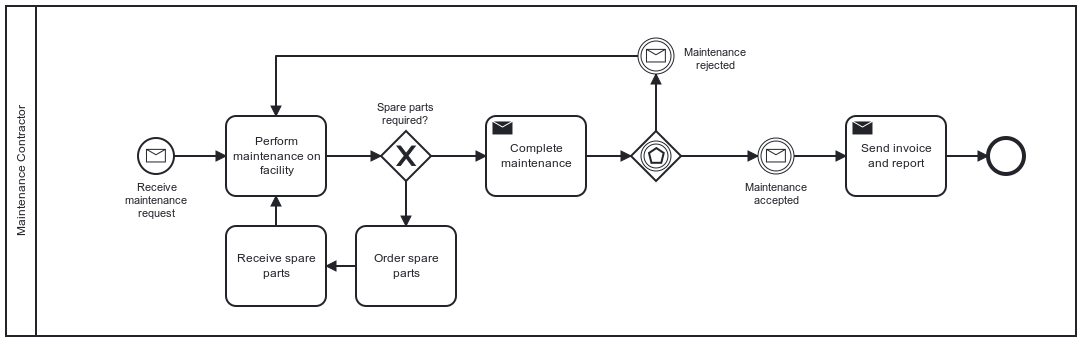
\includegraphics[width=1\textwidth]{background/graphics/maintenance-contractor-only.png}}
    \caption{A simplified business process of a maintenance contractor.}
    \label{fig:background:maintenance_contractor_only}
\end{figure}

This \gls{bpmn} diagram also makes use of some gateways. After the maintainer has performed her first maintenance cycle on the facility, she has to report if any spare parts are required to complete maintenance. If so, spare parts will be ordered; otherwise, the maintenance is complete. For constructs like these, \gls{bpmn} introduces the so-called \textit{exclusive} gateway that only allows execution of one of the subsequent activities. In other words, either the spare parts must have been ordered, received, and replaced in the facilities before maintenance can be completed, or no spare parts are required at all. After maintenance has been completed by the maintainer and thus the maintenance contractor, a third party (in this example, the building administrator) can either accept or reject the maintenance. Waiting for activities of third parties to complete is achieved with the \textit{event-based} gateway. This gateway halts further process execution until one of the subsequent events occurs~\cite{weske2012_bpm_introduction,omg2010_bpmn_by_example}. Single-party \gls{bpmn} diagrams like these are rarely useful because they do not highlight interactions with third parties and, thus, possible conflicts of interest. Introducing a customer as a building administrator into the diagram in figure~\ref{fig:background:maintenance_contractor_only} will improve the example and shows how interactions occur in certain situations. Figure~\ref{fig:background:maintenance_full}\footnote{Created with \url{https://bpmn.io/} (accessed on 2022-11-01)} depicts the full building administrator use case from section~\ref{sec:background:bpm}.

\begin{figure}[h]
    \makebox[\textwidth][c]{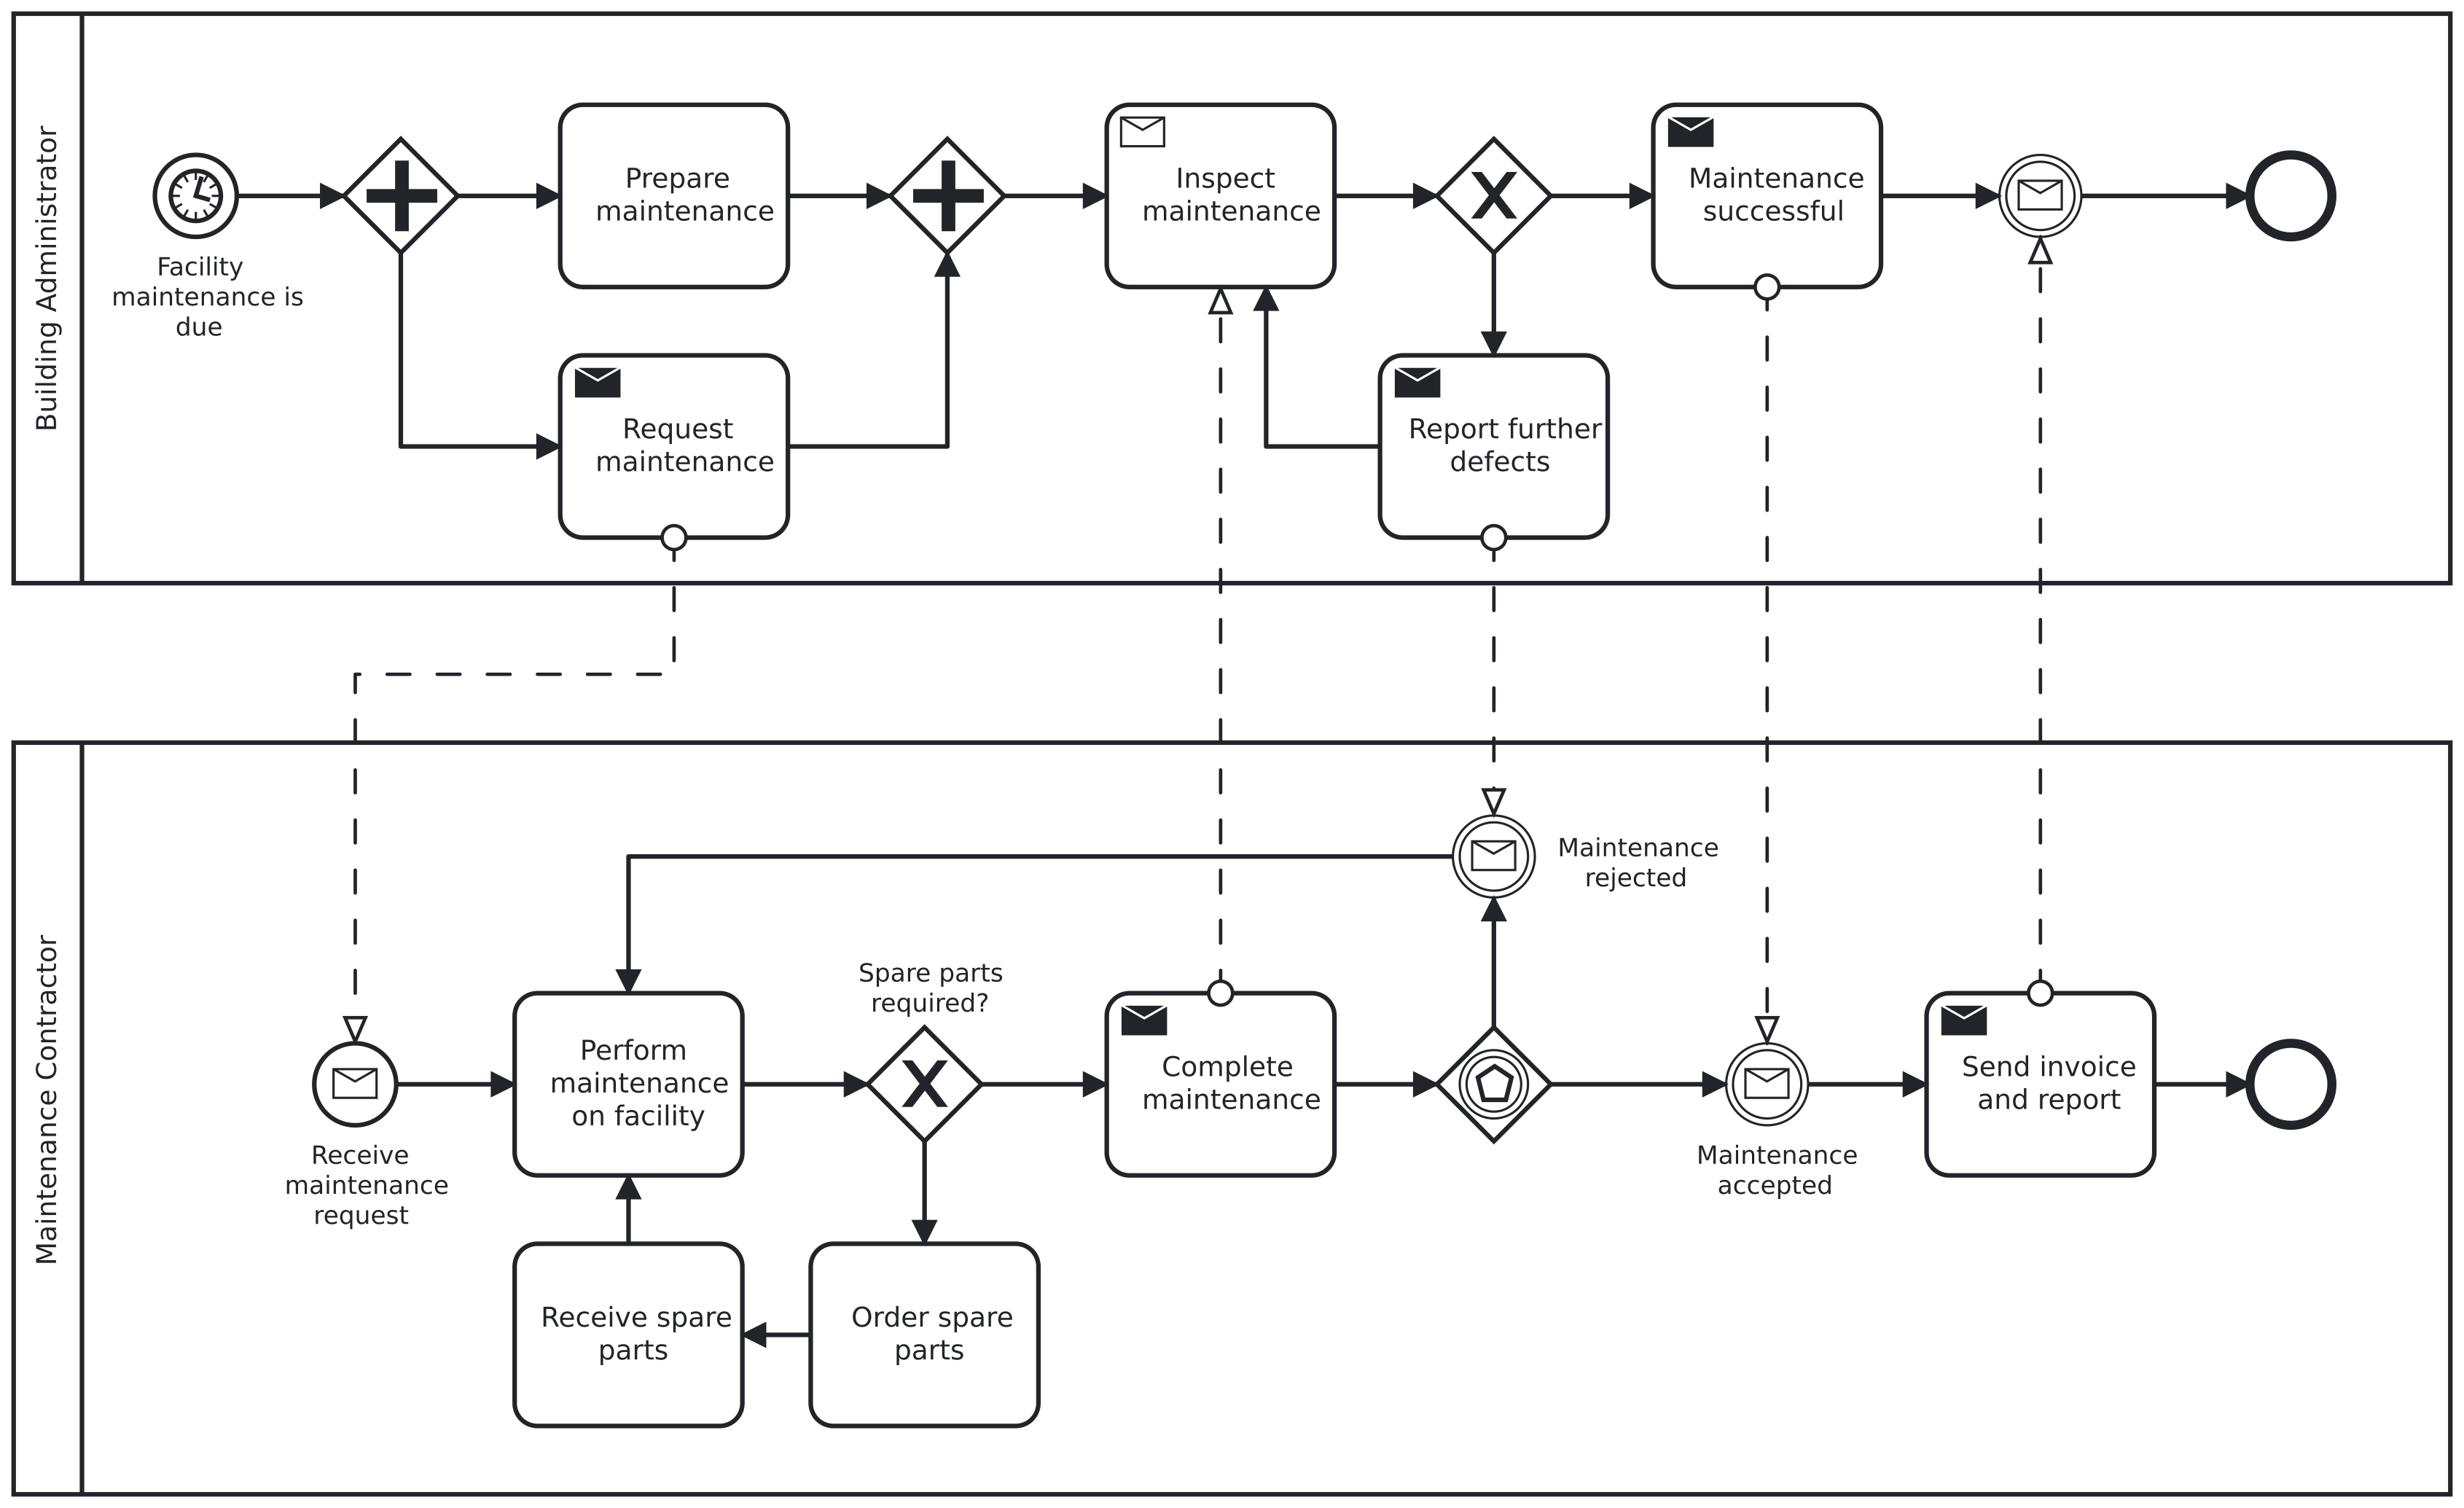
\includegraphics[width=1\textwidth]{background/graphics/maintenance-full.png}}
    \caption{More complex two-lane diagram with interactions between participants.}
    \label{fig:background:maintenance_full}
\end{figure}

The facility maintenance workflow on the side of the building administrator is triggered by the \textit{timer start event} ``facility maintenance is due''. This kind of event indicates that a \gls{bp} should be started whenever the time constraints associated with the event are met. These might be abstract, as depicted in figure~\ref{fig:background:maintenance_full}, or discrete in the form of a timely interval or any other time constraint. When maintenance is triggered, the responsible building administrator has to get in contact with the maintenance contractor and, at the same time, prepares the facility and the building for the upcoming maintenance and notifies staff and local residents (e.g.,\ by sending a notice that the elevator is not available until maintenance is complete). Parallelization of activities in \gls{bpmn} is achieved by employing so-called \textit{parallel} or \textit{split} gateways. A \textit{join} gateway is used afterwards to merge all concurrent branches back together if they have been successfully completed. When maintenance is done, the building administrator inspects the maintainer's work and either certifies the maintenance or reports further defects. Once again, this is achieved by employing the \textit{exclusive} gateway of the \gls{bpmn} notation~\cite{bpmn_v2_spec,weske2012_bpm_introduction}.

% As mentioned before, this example is a greatly simplified \gls{bp} that was derived from real-world \glspl{bp} used by domain experts to visualize some of the concepts introduced by \gls{bpmn}. However, \gls{bpmn} has proven itself as a valuable tool in computer science and business administrations due to its ubiquitous, unambiguous, and well-defined elements. Thus, the remainder of this work also makes use of \gls{bpmn} to introduce and describe other use cases as well.


\subsection{Orchestration and Choreography}
\gls{bpmn} introduces a specification language that allows its users to define \glspl{bp} on a rather granular level using flow and connecting objects. Typically, these objects are grouped into swim lanes where each swim lane defines a single party (e.g.,\ a company or organization). The business process defined for this party is also referred to as \textit{orchestration} or \textit{process orchestration}~\cite{bpmn_v2_spec}. Orchestrations are used to provide a more detailed view of activities (and their associated execution constraints) that interact with both external and internal activities~\cite{orchestration_and_choreography,weske2012_bpm_process_orchestration}. While orchestrations focus on one party's perspective, \textit{choreographies} focus on coordinating interactions between multiple parties. Choreography diagrams that depict a sequence of messages exchanged between parties typically represent a distributed process and activity flow. In other words, the interactions between different orchestrations can be formalized as choreography~\cite{trust_in_service_oriented_ds_through_blockchain,weske2012_bpm_process_choreographies}. Choreography diagrams are especially useful in business-to-business scenarios where activities of one business have to interact and exchange messages with activities from other businesses~\cite{orchestration_and_choreography}. Due to the fact that choreography diagrams are part of the \gls{bpmn} specification, their notations are also quite similar~\cite{bpmn_v2_spec}. Instead of describing activities, choreography diagrams focus on so-called \textit{choreography tasks}. Each choreography task represents the interaction between two or more parties. These tasks are connected with each other by reusing \gls{bpmn} \textit{connecting objects}. The building administrator and maintenance contractor example is depicted as choreography diagram in figure~\ref{fig:background:maintenance_full_choreography}.

\begin{figure}[h]
    \makebox[\textwidth][c]{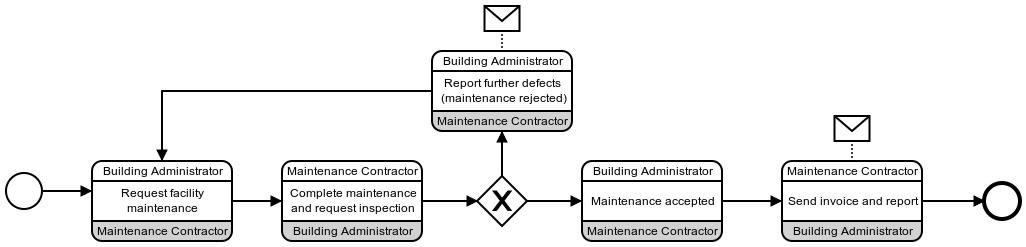
\includegraphics[width=1\textwidth]{background/graphics/maintenance-full-choreography.png}}
    \caption{Choreography diagram highlighting interactions between two participants.}
    \label{fig:background:maintenance_full_choreography}
\end{figure}

Graphically, choreography tasks are denoted with boxes with rounded corners. The inside of the box describes the message exchanged, and two bands, one at the top and one at the bottom of the box, represent the involved parties. The band of the initiating party typically uses the same color as the box itself, whereas the darker band is dedicated to the receiving party. Letter-like symbols connected to the bands of the parties attach supplementary information to the message~\cite{trust_in_service_oriented_ds_through_blockchain,bpmn_v2_spec}. In this example, an invoice and report are added to the last choreography task before reaching the \textit{end event}.

% Besides \gls{bpmn} diagrams, later sections of this work also make use of choreography diagrams to better visualize message exchanges between counterparties and even the blockchain itself.



\section{Baseline Protocol}
\label{sec:background:baseline_protocol}
The Baseline Protocol, a recently defined \gls{eea} standard and OASIS open source project, tries to enable businesses and organizations to synchronize complex \glspl{bp} as well as associated data and messages and increase overall system resiliency. The \gls{bp} introduced in section~\ref{sec:background:bpm:bpmn} is only a simplification of a far more sophisticated scenario. Synchronizing state between counterparties is, therefore, inevitably more difficult than expected. The Baseline Protocol aims to solve this issue by leveraging on the blockchain (or other forms of shared state machines) as an immutable and traceable source of truth that involved participants can trust. Over time, this can increase information security and operational integrity because systems of record no longer have to share potentially confidential data or internal business processes but rely on profound proofs that specific properties of \glspl{bp} have been fulfilled~\cite{baseline_spec}. The standard, however, is still in a volatile state and can introduce breaking changes at any time. Therefore, the upcoming sections only give a rather broad overview of its concepts.


\subsection{Architecture and State Synchronization}
\label{sec:background:baseline_protocol:architecture}
To ensure ``workflow integrity, event ordering, and data consistency'', the Baseline Protocol specifies that a compliant implementation must rely on a \gls{ccsm}. Blockchains like Ethereum and Bitcoin are implementations of such. The systems of record that the \gls{bpi} communicates with are only loosely coupled with the \gls{bpi} itself in the form of a standardized API~\cite{baseline_spec}. Figure~\ref{fig:background:maintenance_multiple_participants} shows a software architecture with a \gls{bpi} integration.

\begin{figure}[h]
    \makebox[\textwidth][c]{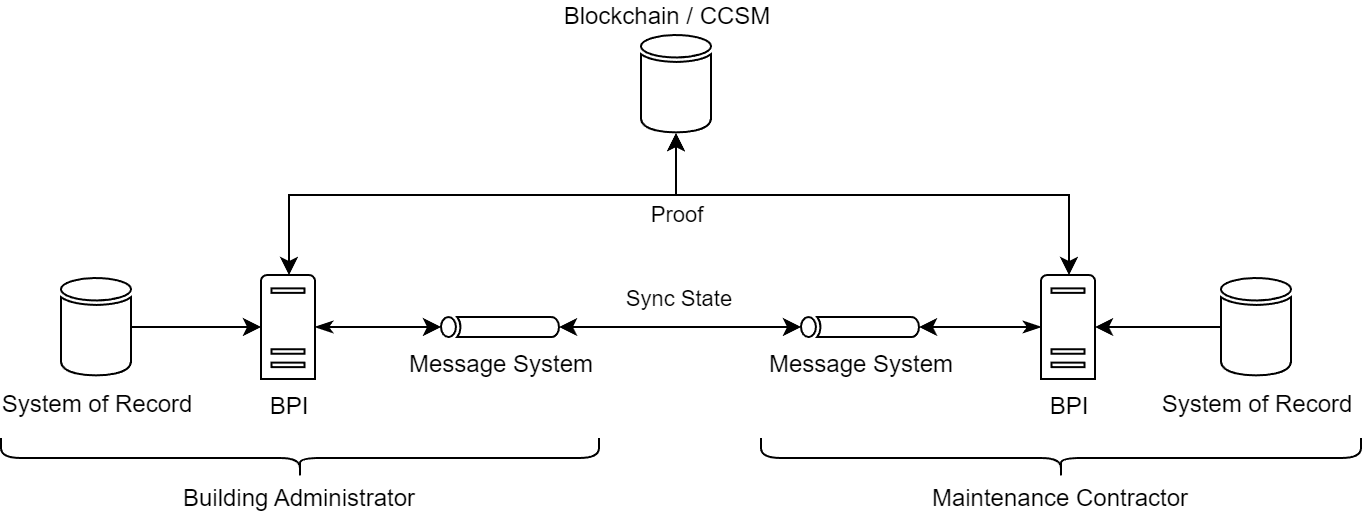
\includegraphics[width=.95\textwidth]{background/graphics/maintenance-baseline-architecture.drawio.png}}
    \caption{Integration of a \gls{bpi} into the two-party facility maintenance system.}
    \label{fig:background:maintenance_multiple_participants}
\end{figure}

All involved participants (the building administrator and the maintenance contractor) keep their own system of record that contains the current state of the workflow, required documents, or even confidential data that is not allowed to leave the organization's network. Communication between participants is solely handled by the \gls{bpi} to exchange necessary information. The \gls{bpi} generates a proof that the document to be exchanged follows the service-level agreements and stores it on a \gls{ccsm} to acquire properties such as traceability, immutability, workflow integrity, or data consistency. On the other hand, the data is transmitted entirely off-chain to keep the smallest footprint possible and reduce transaction cost. This ensures that confidential data can be kept private if necessary and allows sending large amounts of data to counterparties without breaking the blockchains' block size limit. Figure~\ref{fig:background:maintenance_report_baseline} gives a more in-depth explanation of how communication between counterparties can be realized according to the standard and shows the Baseline Protocol compliant process of the maintenance contractor sending the maintenance report to the building administrator in the form of a flow chart. A system of record that wants to take advantage of the properties of the Baseline Protocol at least has to implement the depicted communication.

\begin{figure}[h]
    \makebox[\textwidth][c]{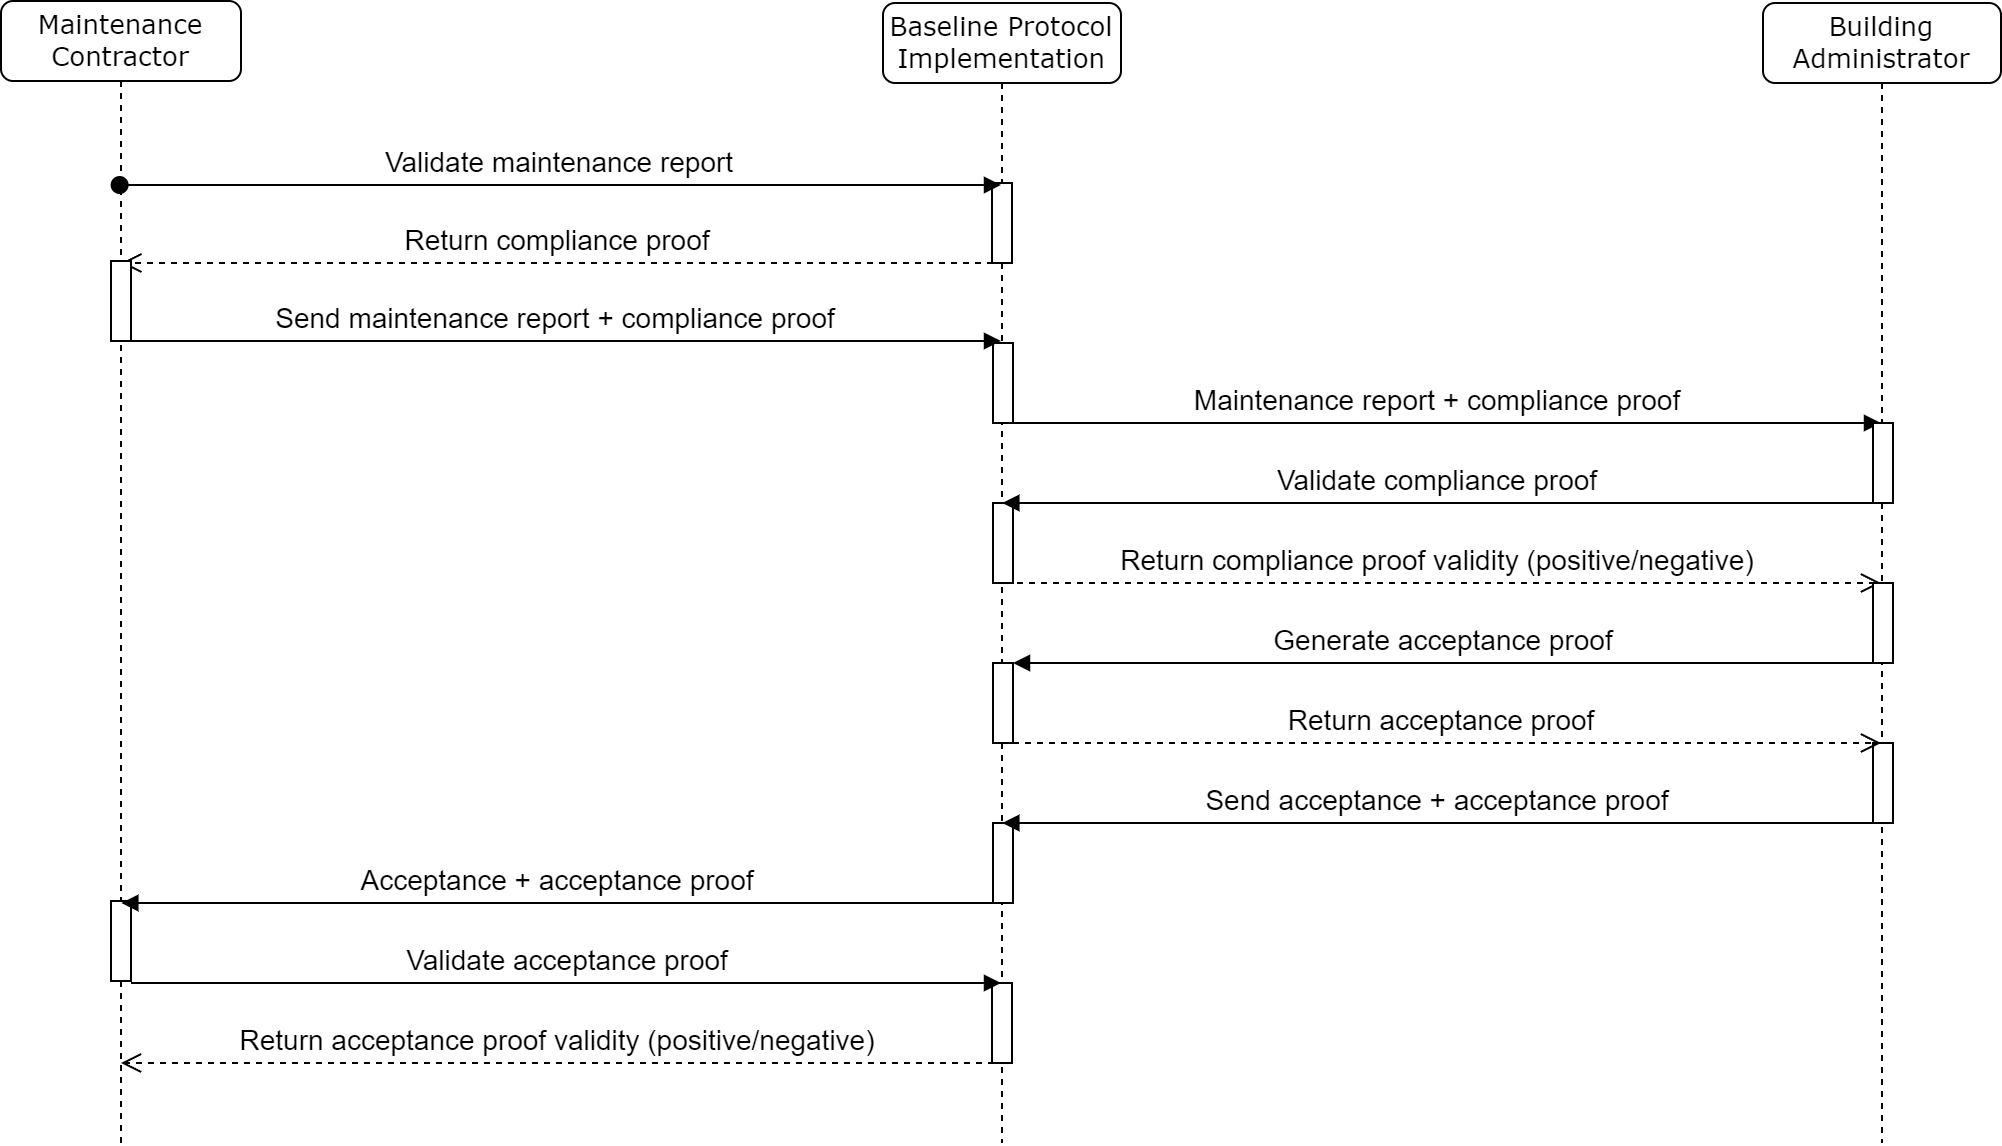
\includegraphics[width=1\textwidth]{background/graphics/maintenance-report-baseline.drawio.png}}
    \caption{Integration of the Baseline Protocol for the exchange of the maintenance report between maintenance contractor and building administrator.}
    \label{fig:background:maintenance_report_baseline}
\end{figure}

After maintenance has been completed, the maintenance contractor sends the maintenance report to the \gls{bpi} API to check its validity. This check is implemented using zero-knowledge circuits\footnote{\glspl{zkp} and ZK circuits are out of scope of this work and will not be further discussed.} that precisely portray the service-level agreements that both parties accepted at the start of the \gls{bp}. If the maintenance report complies, a proof (in the form of zero-knowledge) is returned, and the maintenance report is being transmitted, including the newly generated proof, to the building administrator. Generating proofs, however, is a rather computationally expensive task. Performing it on-chain is therefore unfeasible, considering that hundreds of thousands of proofs must be generated for \glspl{bp} of large companies and organizations. Thus, layer-2 rollup blockchains like Baseledger\footnote{\url{https://baseledger.net/} (accessed on 2022-11-01)} must be employed that are optimized to generate such proofs in a more cost-efficient way. Layer-2 rollups like these, again, only store a \gls{zkp} of the correctness of all \gls{bp} proofs on layer-1 \glspl{ccsm} like Ethereum, to take advantage of the vast amount of participants of such blockchains without exposing any privacy critical data. After receiving the maintenance report with its corresponding compliance proof, the building administrator can now validate the compliance proof to check (1) if the transmitted maintenance report is the one issued by the maintenance contractor and (2) if it is compliant with the previously agreed upon service-level agreement. If the validity check passes, the building administrator can generate a proof that confirms that she accepts the maintenance report in the given form. This proof, once again, can be validated by the other party (in this case, the maintenance contractor)~\cite{baseline_spec}.

Even though the Baseline Protocol is still under heavy development and some of its implementation details are out of scope of this work, given its capabilities, it still holds a lot of potential considering inter-organizational \gls{bpm} and choreographies. Thus, later sections of this work will also investigate possible integrations of the Baseline Protocol into a state machine concept that allows time-traveling verification of \glspl{bp}.


\chapter{Related Work}
\label{sec:related-work}

\newacronym{sla}{SLA}{Service-Level-Agreement}
\newacronym{soa}{SOA}{Service-oriented Architecture}
\newacronym{baas}{BaaS}{Blockchain-as-a-Service}
\newacronym{bpm}{BPM}{Business Process Management}
\newacronym{bpmn}{BPMN}{Business Process Model and Notation}
\newacronym{bct}{BCT}{Blockchain Technology}
\newacronym{bpms}{BPMS}{Business Process Management System}

This chapter will briefly discuss the methodology used to conduct the literature review and outlines relevant related work in the field of business process management that utilizes \gls{bct} to establish properties such as trust and tamper-proofness. At the end of the chapter, the described concepts will be compared with each other and with the proposed approach of this thesis.

\section{Literature Review Methodology}
\label{sec:related-work:methodology}
The following literature review has been performed using the narrative review methodology with its focus on the state of the art~\cite{literature_review_stratton}. Since \glspl{bct}, and especially the utilization of \glspl{bct} in the area of \gls{bpm}, are rather new research topics, only literature of the last 10 years (i.e.,\ 2012 -- 2022) is considered relevant. The literature review is used to answer RQ1. Table~\ref{tab:literature_review_keywords} shows a list of primary, secondary and tertiary search terms that were used during the narrative review in the databases of \textit{Elsevier}, \textit{Springer}, \textit{IEEE} and \textit{Researchgate}.

\begin{table}[h]
\centering
\begin{tabular}{|c|c|c|}
    \hline
    \textbf{A} & \textbf{B} & \textbf{C} \\
    \hline
    \makecell{Blockchain} &
    \makecell{Collaborative\\Choreography\\Inter-organizational} &
    \makecell{Business Process\\Business Process Management} \\
    \hline
\end{tabular}
\caption{Search terms used during the narrative review}
\label{tab:literature_review_keywords}
\end{table}

The formal definition on how these search terms were combined is shown in equation~\ref{eq:literature_review_keyword_combination}.

\begin{equation}
E = [(\bigvee_{1 \leq i \leq 1} A_{i}) \wedge (\bigvee_{1 \leq i \leq 3} B_{i})] \wedge (\bigvee_{1 \leq i \leq 2} C_{i})
\label{eq:literature_review_keyword_combination}
\end{equation}

Narrative literature reviews do not claim (semi-)completeness on the coverage of a certain topic but give more of a rather unstructured overview of what already exists~\cite{literature_review_rhoades}. Systematic literature reviews such as~\cite{slr_collaborative_bpm_using_blockchain} found using equation~\ref{eq:literature_review_keyword_combination} were used as starting point. Furthermore, the snowballing approach was applied to extract primary sources. % chktex 36


\subsection{Untrusted Business Process Monitoring and Execution Using Blockchain~\cite{untrusted_bp_execution_using_blockchain}}

The ground-laying work for business process execution utilizing the blockchain published by Weber et al.\ (regularly cited in subsequent work such as~\cite{runtime_verification_for_bp_utilizing_bitcoin,bo_collaboration_between_healthcare_providers_covid_19,caterpillar_blockchain_based_bpm_system,modeling_blockchain_based_choreographies,blockchain_based_information_sharing_in_io_workflows}), aims to find agreements between counterparties on a shared state without the use of a trusted third party. In their exemplary use case, the authors outline a situation where a manufacturer orders supplies via a middleman, and the entire supply chain gets delayed because of production issues on the suppliers' side. Due to the delay, the manufacturer now refuses to accept the supplies from the carrier, which makes the carrier eligible for compensational payments from the supplier or the middleman. To tackle common~\cite{impact_of_trust_on_supply_chains}, trust-related, supply chain issues like these, Weber et al.\ suggest the integration of business processes into \gls{bct}. Their approach is split into design and run-time decisions. During design-time, a formal model of the business process has to be outlined using a description language similar to \gls{bpmn} or more blockchain-specific alternatives such as the one described by Ladleif et al.\ in~\cite{modeling_blockchain_based_choreographies}. This model is then translated into a factory smart contract containing all relevant business process information. The component-based design of this concept allows implementers to use custom translators, such as the one described by Nakamura et al.~\cite{inter_organizational_bps_managed_by_blockchain}, as well. During run-time, the factory smart contract is used to instantiate and deploy instance contracts that additionally contain information about the roles of the participants (which might not be obvious during design-time). Participants only communicate with each other (and send data) through the blockchain and the deployed instance contracts. These contracts are available in two different forms: (1) a \textit{choreography monitor}, which will check conformance with the business process, and (2) an \textit{active monitor} which is an extension of the \textit{choreography monitor} and can perform additional data transformations or calculations on-chain. Which one to choose depends on the use case and if the data is encrypted. Instance contracts hold and advance the status of the business process and the choreography rules and can trigger external APIs using \textit{triggers}. Triggers are programs that run on full-nodes and listen to smart contract events. Participants will then further process data off-chain that was sent over the blockchain. Due to the payload limitations of transactions on blockchains like Ethereum~\cite{ethereum_yellow_paper}, only smaller payloads might be transferred directly. For larger payloads, just the hash of the data is attached to the transaction, and the data itself is made available using off-chain storage solutions such as Amazon S3\footnote{\url{https://aws.amazon.com/de/s3/} (accessed on 2022-11-29)} or Google Cloud Storage\footnote{\url{https://cloud.google.com/storage} (accessed on 2022-11-29)}.

However, the on-chain logic and complexity of business processes are limited due to the 24 KB size limit of smart contracts on Ethereum~\cite{ethereum_yellow_paper}. This issue can be circumnavigated by applying the \textit{diamond pattern}\footnote{\url{https://eips.ethereum.org/EIPS/eip-2535} (accessed on 2022-11-29)}, but will inevitably add overall complexity and cost due to the increased amount of smart contracts that have to be deployed. For fairness, the authors suggest that participants may want to split gas money (including smart contract deployments) differently rather than relying on the implicit split of the business process itself. For their prototype, Weber et al.\ rely on the public Ethereum blockchain. In their benchmarks, the authors ran around 7932 transactions in 32 instances where each business process executed from start to end produced costs of around $0.0347$ Ether, which, in 2016, translated to around $0.40$ USD but are $109.49$ USD at the time of writing this work in 2022. With the fluctuation of prices of cryptocurrencies~\cite{predicting_cryptocurrency_price_bubbles,monitoring_financial_stability_cryptocurrencies}, conflicts between counterparties might be an aspect to consider when running long-term business processes. Regarding privacy, the authors suggest the usage of asymmetric encryption of data transferred over the blockchain or to rely entirely on permissioned blockchains. Private permissioned blockchains, however, are typically less accepted by industry partners~\cite{public_chains_make_private_chains_obsolete}, which will lead to centralization and thus nullifies the advantages of blockchains in the first place.

The authors utilized and extended upon their approach to implement a prototypical \gls{bpms} as proof-of-concept called Caterpillar\footnote{\url{https://github.com/orlenyslp/Caterpillar} (accessed on 2022-11-29)}. Caterpillar allows the factory and instance smart contract creation from \gls{bpmn} models and deploys them on the blockchain. When generating smart contracts from \gls{bpmn}, the system creates an intermediary representation of the business process using Petri nets to allow further optimization of the created smart contracts~\cite{optimized_execution_of_bp_using_petri_nets_on_blockchain}. Furthermore, their system exposes a REST API to make working with business processes more convenient~\cite{caterpillar_blockchain_based_bpm_system,caterpillar_bp_execution_engine_on_eth}.


\subsection{An Architecture for Multi-chain Business Process Choreographies~\cite{architecture_for_multi_chain_bp_ladleif}}

Leveraging on the aforementioned concept of Weber et al.~\cite{untrusted_bp_execution_using_blockchain}, Ladleif et al.\ presented a software architecture that aims to enable the usage of different blockchain technologies (e.g.,\ Ethereum, Hyperledger, Tezos, and others) in a single business process instance. To achieve this goal, the authors only used the blockchain and its smart contracts to store the state and all allowed state transitions of a business process instance. The event and transaction logs provided by most blockchain implementations with smart contract capabilities are used to verify if the \glspl{sla} are fulfilled. To enable multi-chain capabilities, the \textit{adapter} software design pattern is utilized where each blockchain, that participants want to integrate, has to implement its own adapter that is able to generate smart contract code, deploy it autonomously and interact with it later on. In most choreographies, not all participants are required to be part of each individual sub-process. Therefore, the system itself determines which parts are relevant for each participant and only connects to the respective smart contracts and blockchains. 

The presented concept gives involved participants more freedom over which blockchain to choose and therefore allows for a more fine-grained adjustment of levels of confidentiality or risk tolerance. Being able to combine different blockchains in a single choreography might be a desirable property depending on the use case and the business needs. Nonetheless, cross-chain communication is still an open problem that might increase the complexity of such a system unnecessarily. Thus, one must consider whether such a system is appropriate for the business process in use.


\subsection{Runtime verification for business processes utilizing the Bitcoin blockchain~\cite{runtime_verification_for_bp_utilizing_bitcoin,prybila_master_thesis}}

The conceptual model and the prototype presented by Prybila et al.\ aim to utilize and integrate business processes directly into the Bitcoin blockchain. Therefore, establish trust between counterparties by enabling time-independent verifiability of decentralized choreographies. Their rather flexible approach to this problem allows the process owner to select participants during runtime. This is a useful trait to have considering long-running processes where participants may drop out or get replaced due to changing requirements. At the start of a new business process, the process owner has to select a free Bitcoin transaction output\footnote{While Bitcoin transaction inputs determine how much value is transferred from one or more addresses, Bitcoin transaction outputs determine to which addresses the value is sent. Typically the input value is larger than the output value. This difference is the block miners reward.} which is used as control token. This control token will be handed over (by using a Bitcoin transaction) to the party that has to perform the next task (i.e.,\ the token holder is fully responsible for the continuation of the business process). In order to enable parallelization of tasks, this concept not only allows process-start, -end, and -handover transactions but also -split and -join transactions. A process-split transaction is performed by the current token holder and contains $1$ to $N$ new process tokens in the form of Bitcoin transaction outputs. The new token owners perform their tasks before joining the process back together. It is assumed that a single process-split corresponds to exactly one process-join later on. The authors defined a process-end transaction as a transaction with only a single input which means that a process-join must be performed before a process can complete (if the process was split earlier on). To define the different enriched transaction types, the \textit{data output} and the \textit{Pay-to-Script-Hash} standard Bitcoin transactions are used. The latter of both can carry additional data if necessary. The data will be transferred off-chain, and the transaction itself will only include a hash of the data due to privacy concerns and the fact that Bitcoin is a public permissionless blockchain. Due to the process timestamps and the publicly available data on the blockchain, process owners can monitor the progress of the entire business process and even of single tasks if made available by the current control token owner. The immutability of data on-chain allows the process owner to monitor the progress and verify if predefined \glspl{sla} are fulfilled accordingly.

Due to a median transaction confirmation time of around 7.74 minutes of Bitcoin measured by the authors, only long-running business processes and tasks are viable~\cite{runtime_verification_for_bp_utilizing_bitcoin}. However, their concept also includes a \textit{greedy mode} that allows handover of the control token even if a transaction was not yet confirmed and included in a block. This is because Bitcoin miners accept transactions with references to other, still pending, transactions~\cite{nakamoto2009}. \textit{Greedy} transactions, however, pose the threat of being entirely dropped if something goes wrong or malicious participants propose alternative handover transactions. Thus imposing possible consistency issues upon the entire business process and making \textit{greedy mode} practically unviable if trust is of utmost importance. The use of the Bitcoin network itself is also questionable because newer, second-generation blockchains, such as Ethereum, provide Turing-complete scripting languages that can depict requirements directly on-chain and can be used to share digital assets between organizations more easily~\cite{bo_collaboration_between_healthcare_providers_covid_19,buterin2020,ethereum_yellow_paper}. Also the way data is transferred between participants might pose certain security issues. Once written to the blockchain, the hash cannot be changed and will be available to the public as long as the blockchain itself is available. Even though not a main concern, malicious participants could still abuse this fact at a later point in time and present different data by using collision attacks posing certain security and trust issues. Data once hashed using MD5 or SHA-1 might no longer be reliably verifiable~\cite{new_collision_attack_on_md5,first_collision_for_full_sha_1}.


\subsection{Blockchain-oriented Inter-organizational Collaboration between Healthcare Providers to Handle the COVID-19 Process~\cite{bo_collaboration_between_healthcare_providers_covid_19}}

Ilyass El Kassmi and Zahi Jarir presented a conceptual model with a proof-of-concept implementation to handle trust issues when sharing sensitive data in the healthcare sector on a national scale. The authors oriented themselves on a large-scale pandemic use case regarding COVID-19. This concept is especially interesting because it aims to deal with large amounts of data, a changing business process, and privacy concerns. However, it does not focus on the security aspects. To handle ever-changing business processes, the authors use finite state automata modeling and map the model to a \gls{soa} to abstract functional and non-functional requirements onto the software architecture. The blockchain, in this case, Hyperledger, is dynamically plugged into the system as a third-party service that introduces a new level of indirection. This \gls{baas} approach allows for other blockchains to be used as well and enables a higher level of decentralization since private permissioned blockchains are typically considered to be more centralized since network maintainability is typically ensured by one authority only. The authors introduced the blockchain to depict non-functional requirements, like enabling trust for inter-organizational collaboration only. In this approach, blockchain interactions are seen as a way to fulfill those predefined behavioral non-functional requirements. After processing a workflow step locally, the \gls{soa} will forward certain sub-tasks to the blockchain and corresponding smart contracts. Other participants will (automatically) react to those changes in the smart contract and dispatch new events themselves if necessary. In the case of their COVID-19 use case, this might be a PCR test result published by the regional epidemiological center that, depending if the test was positive or negative, is being further processed by the governmental healthcare provider.

Although this novel approach fits this specific use case, it does not generalize well. The authors conclude, that it still heavily depends on the chosen blockchain platform and its limitations in terms of security, scalability, performance, and other key aspects. This might cause issues, especially with short-running business processes. The usage of permissioned blockchains also comes with certain restrictions. Due to the small number of participants compared to public permissionless blockchains, misuse of the blockchain by one participant could render the system untrustworthy because it entirely relies on the integrity of the collaborators~\cite{lamport2002,sousa12from_byzan_consen_bft_state_machin_replic}. Hence, the proposed approach assumes a form of common interest in which all members trust each other to at least some extent. Using public permissionless platforms in this context might be viable for use cases where data privacy is not of utmost importance. This, however, cannot be said about healthcare-related data. The authors directly encoded information about the patient and her COVID-19 process into the smart contracts. This means that the information would be publicly available to anybody on a public permissionless blockchain, which contradicts the GDPR\footnote{\url{https://gdpr.eu/} (accessed on 2022-11-13)}. Thus, other storage solutions have to be applied if privacy critical data has to be shared with counterparties.


\subsection{Blockchain-based controlled information sharing in inter-organizational workflows~\cite{blockchain_based_information_sharing_in_io_workflows}}

Rondanini et al.\ inspired their work by the trust problems associated with sharing information in inter-organizational scientific choreographies. Especially when APIs of counterparties and other participants have to be consumed, ensuring that the least privilege principle\footnote{A participant is only given exactly those privileges needed to complete a task.} is being followed, might be of utmost importance. To achieve this goal, the authors solely rely on the distributed consensus algorithm of blockchains to guarantee a correct order of execution of business processes (as shown in~\cite{blockchain_for_secure_io_bp}). They split their smart contracts into two layers that are tightly coupled with each other: (1) The \textit{coordination layer} that ensures a correct order of execution of the choreography and (2) the \textit{authorization layer} that handles resource access on a per sub-task basis. To be more specific, the authors tackle temporal authorization management (authorization can be revoked) and the least privilege principle with their novel concept. On choreography initialization and smart contract deployment, each participant has to announce, in the form of transactions with a specific payload format, which resources (for example, APIs) they provide. When participants want to start working on a certain sub-task of the business process, they have to send a transaction containing all required resources to the smart contract that handles this sub-task. The smart contract will then check which resources are applicable and grants access. The resource providers listen to the smart contracts event log and will automatically toggle access to their off-chain resources for this particular participant. The smart contract will revoke resource access once the sub-task executor announces that their work has been completed. Later on, participants can check what kind of resources counterparties used by examining the log of transactions during execution.

The authors' approach to the least privilege principle and the trust problems associated with choreographies allows for automated authorization management and post-execution verifiability of business processes. However, their concept requires choreographies to be relatively inflexible. Participants have to be assigned to sub-tasks they will work on before the business process even starts. Due to the properties of blockchains and transactions, once revealed, resources cannot be revoked either. Drawbacks like these might have severe consequences, especially for long-running business processes where organizations have to comply with changing legal requirements. Revoking access to resources only off-chain might break the entire business process if other participants still require those resources to complete their sub-tasks.


\subsection{A Lean Architecture for Blockchain Based Decentralized Process Execution~\cite{lean_architecture_for_blockchain_based_process_execution}}

In their work, Sturm et al.\ try to leverage on the work of Weber et al.~\cite{untrusted_bp_execution_using_blockchain} by generalizing the smart contracts in use for a ``source-code optimized solution'' that is open for extension if necessary. The smart contract is deployed per instance of a business process and only serves as scaffolding. This scaffolding smart contract holds a list of participants and sub-tasks where each sub-task contains a description of the action that has to be performed, the wallet address of the participant that is allowed to complete the task, and a list of predecessor tasks that must be completed before this task can be tackled. After the scaffolding smart contract deployment, the participants and the tasks are added using functions defined in the contract (i.e.,\ blockchain transactions). To partially conform with \gls{bpmn}, tasks can be defined (1) as simple \textit{TASK}, which only has one predecessor, (2) as \textit{AND}-task, where a list of predecessors has to be completed, or (3) as \textit{OR}-task, where at least one of the predecessor tasks has to be completed before the task itself can be completed. The formal definition of the function $C(t)$ that checks if task $t$ can be completed is depicted in equation~\ref{eq:lean_architecture_complete_condition}.

\begin{equation}
    C(t)=\begin{cases}
        C(P_t) & \text{for simple tasks} \\
        \bigwedge_{t_p \in P_t} C(t_p) & \text{for \textit{AND}-tasks} \\
        \bigvee_{t_p \in P_t} C(t_p) & \text{for \textit{OR}-tasks}
    \end{cases}
    \label{eq:lean_architecture_complete_condition}
\end{equation}

Where $P_t$ is the set of predecessor tasks and $C(t)$ is defined as recursive function. The authors circumnavigated the recursiveness by adding a \textit{completed} flag to each task to prevent the smart contract from performing redundant computation on-chain. The capabilities of error handling in Solidity, the smart contract programming language of Ethereum, specifically allows participants to communicate with the smart contract more directly. Thus, the authors were able to create a cleaner concept compared to~\cite{untrusted_bp_execution_using_blockchain}. Due to the way the scaffolding smart contract works, Sturm et al.\ proposed, that for their concept, a \gls{bpmn} translator would not output smart contract code directly, but would generate a list of blockchain transactions that add participants and tasks that depict the business process itself.

This concept tries to solve the lack of trust in choreographies between counterparties by storing as much information on-chain as possible. The authors even mention, that they do not want to rely on off-chain storage solutions. Thus, even large files and datasets would be attached to tasks on-chain. Not only could the transaction and block size limit cause issues, but participants might also be concerned with privacy regarding their data being published. To deal with associated privacy and security issues, the authors recommend the usage of consortium blockchains\footnote{Blockchains where all miners/validators are predefined and cannot change.}. However, consortium and private blockchains will inevitably weaken the tamper-proofness to some extent because the voting power is concentrated to preselected nodes. Another disadvantage of this approach is that it relies on the inflexibility of its business processes. Due to the immutability of blockchain transactions~\cite{nakamoto2009}, tasks and participants cannot be changed in the proposed concept. Even though the scaffolding smart contract could be extended to allow such behavior, the authors did not establish a sound concept of how participants agree to changes in the process.


\subsection{Interpreted Execution of Business Process Models on Blockchain~\cite{interpreted_bp_on_blockchain_weber}}

Concepts where \gls{bpmn} models are compiled to smart contracts (as proposed in~\cite{untrusted_bp_execution_using_blockchain,bo_collaboration_between_healthcare_providers_covid_19,blockchain_based_information_sharing_in_io_workflows}) do have certain flexibility limitations. To overcome these limitations, López-Pintado et al.\ proposed a concept that utilizes smart contracts to interpret business processes on the blockchain, similar to the previous work of Sturm et al.~\cite{lean_architecture_for_blockchain_based_process_execution}. To reduce the footprint on the blockchain and allow dynamic modification of the business process during run-time, the authors recommend the usage of a space-optimized tree-like data structure that encapsulates the workflow. Even though the interpreter that encodes the \gls{bpmn} semantics only has to be deployed once, each sub-process that participants want to add to the choreography will automatically deploy additional smart contracts (one responsible for the sub-process workflow and another one holding associated model data). Therefore, the proposed concept cannot scale well due to the vast amount of associated contracts deployed~\cite{interpreted_bp_on_blockchain_loukil}. Furthermore, allowing participants to dynamically modify the workflow data structure during run-time might lead to consistency issues (e.g.,\ due to the order in which transactions are accepted by the blockchain~\cite{nakamoto2009,ethereum_yellow_paper}). Even though the concept enables access restrictions for participants, modification might still lead to inconsistent state. The usage of systems, that should establish trust between counterparties, but might still produce inconsistent state on the blockchain, is questionable. Participants might see different state representations of the same business process, which nullifies the usage of blockchain in the first place.


\subsection{Decentralized Collaborative Business Process Execution Using Blockchain~\cite{interpreted_bp_on_blockchain_loukil}}

Building upon the work of~\cite{lean_architecture_for_blockchain_based_process_execution} and~\cite{interpreted_bp_on_blockchain_weber}, Loukil et al.\ aim to further reduce the inflexibility of business process management on the blockchain with their concept. To achieve this goal, three types of smart contracts are deployed in a 3-layer architecture. The central smart contract is called the \textit{interpreter}. It is only deployed once, holds references to the \textit{business process instance} and the \textit{resource instance} smart contracts and implements the facade pattern\footnote{\url{https://en.wikipedia.org/wiki/Facade_pattern} (accessed on 2022-11-13)} to access the business process. When a business process is triggered, the interpreter generates a new business process instance smart contract. Participants then dynamically add the \gls{bpmn}-based configuration to the newly created smart contract through the interpreter using blockchain transactions. Similarly to the business process instance smart contract, the resource instance smart contract that holds and manages the roles of participants, is also generated by the interpreter itself. As mentioned before, these smart contracts are embedded in a 3-layer architecture. The first layer, the \textit{conceptual layer}, is solely responsible for translating \gls{bpmn} models to an intermediary JSON representation to be more blockchain agnostic. The JSON configuration is then fed into the interpreter smart contract that is part of the \textit{data layer}. The data layer statically encodes a basic business process workflow data structure that is the same for all instances. The routing logic and the process workflow are added to the created business process instance smart contracts in the \textit{flow layer}. Business process instance and resource instance smart contracts can only be accessed and configured by the interpreter. This gives the interpreter more leverage over the entire choreography and enables handling whether or not certain participants are allowed to perform certain tasks or if they are allowed to modify the roles or the business process itself.

The evaluation of the concept shows that business process instance deployment typically leads to higher costs regarding gas compared to compiled approaches such as the one proposed by Weber et al.~\cite{untrusted_bp_execution_using_blockchain}. The tight coupling and integration with the blockchain itself also leads to a dependence on the chosen blockchain technology regarding the transaction confirmation time. These two aspects make the concept rather disadvantageous for short-running business processes where many business process instance and resource instance smart contract deployments are required, and state transitions must be performed quickly. Similarly to other proposals, the authors of this concept are also reluctant to tackle the privacy concerns of participants. They advise the usage of consortium blockchains to keep the business process and the associated data private. However, due to the capabilities of the approach to change participants and their roles during run-time, consortium blockchains will inevitably lead to more management overhead since new participants are advised to run their own full node of the blockchain. If participants decline, the usage of blockchain becomes questionable due to security issues like 51\% attacks opening up. Nonetheless, the novel architecture presented by the authors gives opportunity for future work to tackle the issues mentioned above, and its loose coupling allows the integration of other approaches as well.


\subsection{Inter-organizational Business Processes Managed by Blockchain~\cite{inter_organizational_bps_managed_by_blockchain}}
\label{sec:related-work:nakamura}

Due to certain limitations of blockchain technologies like throughput, latency, or size restrictions, Nakamura et al.\ proposed a statechart transformation algorithm for \gls{bpmn} that allowed the authors to bring down the number of dispatching and receiving events by up to 74\% and 65\%. Their approach is structured in three subsequent steps. In the first step, a \gls{bpmn} model is transformed into one statechart for the shared business process on the blockchain and one statechart for each participant. Each statechart represents all states a participant can be in and all corresponding state transitions where state transitions are triggered in the form of events dispatched by any of the participants involved. The authors define a state transition as $e/a_1,\ldots,a_n$ with $e,a \in E$ where $E$ is the set of events that may occur in the business process, $e$ being the receiving event (that starts the state transition) and $a_1,\ldots,a_n$ being the events dispatched after the state transition is completed. Thus, a statechart can be formalized as 5-tuple $\langle S, s_0, F, E, T \rangle$ where S is the set of possible states, $s_0 \in S$ the initial state, $F \subseteq S$ being the set of final states and $T$ is the set of transitions. An event dispatched by the statechart of the shared business process on the blockchain might be used as a state transition starting event for the statechart of one of the participants and thus allows communication between independent statecharts solely relying on a predefined set of events $E$ that all participants share. The proposed algorithm reduces the produced statecharts in the second step. The authors focus on two consecutive state transition where none of them dispatches any events on completion (as depicted in equation~\ref{eq:consecutive_state_transitions_without_dispatching_events}).

\begin{equation}
    s_1 \xrightarrow[]{e_1/\emptyset} s_2 \xrightarrow[]{e_2/\emptyset} s_3
    \label{eq:consecutive_state_transitions_without_dispatching_events}
\end{equation}

Suppose the first state transition from $s_1$ to $s_2$ is removed (including the receiving event $e_1$ that triggers the transition) and the statechart is rewritten to only allow immediate transitions from $s_1$ to $s_3$ using $e_2$ as starting event (as depicted in equation~\ref{eq:consecutive_state_transitions_without_dispatching_events_reduced}). In that case, the observed behavior from outside the statechart will not change because neither less nor more events are being dispatched, and the resulting state is the same.

\begin{equation}
    s_1 \xrightarrow[]{e_2/\emptyset} s_3
    \label{eq:consecutive_state_transitions_without_dispatching_events_reduced}
\end{equation}

This transformation will not only allow the removal of the no longer used state $s_2$ but will also allow the removal of the dispatching event $e_1$ if and only if no other participant or the shared business process itself requires it. One might even consider a generalization of the transformation algorithm for more than two consecutive state transitions without dispatching events as well. The third step proposed by Nakamura et al.\ then includes a transformation of the statecharts to smart contracts and automatically generated web user interfaces that allow interaction with the business process.

Even though this novel approach only considers consecutive state transitions and does not include process forks and joins such as the concept proposed by Prybila et al.~\cite{runtime_verification_for_bp_utilizing_bitcoin,prybila_master_thesis}, the algorithm still holds potential for adaptation in future work due to the vast reduction of dispatching events and the extraction of a dedicated statechart representing the interactions with the blockchain.


\subsection{Data-Driven Process Choreography Execution on the Blockchain: A Focus on Blockchain Data Reusability~\cite{data_driven_choreography_data_reusability_lichtenstein}}

An approach that focuses more on the artifacts produced by a business process and their reusability across instances, was proposed by Lichtenstein et al. The authors' concept focuses on three smart contract types that loosely interact with each other. The first smart contract is the \textit{participants interface}. These interfaces are deployed by each participant involved in the choreography individually and only expose functionality that is relevant for the respective participant to advance the business process instance. The participants' interface further communicates with the \textit{data object store}. This kind of smart contract is deployed once per choreography, holds an instance ID that is increased for each new instance of a business process, and references all required \textit{data object} smart contracts. The data objects are use case and domain-specific smart contracts that depict certain business process artifacts\footnote{Imagine a car rental business process. In such a scenario, typical data objects would be the car, the driver's license, or the order with its corresponding invoice. Each data object has its own lifecycle with its own custom properties.}. These data objects are reused throughout multiple business process instances, which will reduce the number of smart contracts deployed per business process instance dramatically compared to other concepts such as the one proposed by Weber et al.~\cite{untrusted_bp_execution_using_blockchain} or the one proposed by Ilyass El Kassmi and Zahi Jarir~\cite{bo_collaboration_between_healthcare_providers_covid_19}. Data objects are modified through the participants' interface and directly represent the current state of the business process instance. This decoupling of process logic and data objects allows the reuse of data objects in new business process instances and even across choreographies. Therefore, new choreographies with a different process logic and different participant interfaces can import \textit{external} data objects that were produced by other choreographies previously. These external data objects can be used as an additional source of information for newly deployed choreographies.

The dynamic approach proposed is highly beneficial for short-running choreographies where similar business processes are instantiated regularly. Even though the deployment cost is typically higher compared to similar approaches due to the vast amount of data object smart contracts required, the authors could still show a linear decrease in business process instantiation cost. This is due to the circumstance that other approaches deploy all required smart contracts per business process instance, while the approach proposed by Lichtenstein et al., reuses all smart contracts and only has to increase a single variable per instantiation in the data object store. Nonetheless, the approach lacks access rights management and the option to encrypt sensitive data. Thus, further research still has to be conducted considering that data objects are on-chain, and their progression throughout a business process instance is of utmost importance for this approach.


\subsection{Modeling and Enforcing Blockchain-Based Choreographies~\cite{modeling_blockchain_based_choreographies}}

Most of the aforementioned concepts rely on choreography or business process diagrams defined in the \gls{bpmn} 2.0 standard. However, choreography diagrams are regarded to be purely descriptive and thus lack properties required in model-driven engineering to allow process execution. Moreover, the current standard of \gls{bpmn} does not reflect most blockchain capabilities directly. Thus, Ladleif et al.\ proposed a fully backwards-compatible extension to \gls{bpmn} 2.0 choreography diagrams that enable execution by adapting existing and introducing two new elements that allow the representation of data and logic directly on the blockchain. Data is being stored and shared between participants using two different concepts:

\begin{itemize}
    \item \textit{Message exchanges}: Messages that are attached to choreography tasks, and are either sent by the task initiator or the task respondent, are represented by blockchain transactions. Due to the circumstance that all transactions are automatically attached to the immutable event log of the blockchain, all participants can verify the state of the choreography at a later point in time. Messages are converted to byte sequences by the client to allow arbitrary data structures being exchanged.
    \item \textit{Data objects}: The rather artifact-centric approach of this concept introduces so-called \textit{data objects} in the form of variables inside choreography smart contracts. This gives participants more flexibility when sharing information for the progression of the choreography. The append-only data structure that a blockchain is, allows participants to verify if necessary information was shared and if the data objects have been in the correct state to allow a specific state transition, for example.
\end{itemize}

To ensure correctness of the choreography, smart contracts directly embed the control flow logic derived from the choreography diagram. The extension, however, also allows participants to define custom logic in the form of script tasks. These script tasks can access message logs or data objects to check if a task can be completed or if the next task can be started. To enable authorization management and verify if certain participants are allowed to perform state transitions in the choreography, the authors proposed using an additional smart contract called the \textit{participants registry} where each participant has to be registered prior to choreography instantiation.

Even though the proposed concept performs well regarding correctness of the choreography, traceability, and run-time verification, flexibility is still an issue due to the immutability of smart contracts and, thus, not being able to extend or change data objects once deployed and in use. Even though patterns exist for changing data objects (as proposed by Lichtenstein et al.~\cite{data_driven_choreography_data_reusability_lichtenstein}), the integration is still an open problem due to the tight coupling of logic, data objects, and smart contracts. Another issue discussed by the authors is the current limitation of smart contracts not being able to trigger tasks automatically, which is a valuable property, given that the choreography relies on recurring tasks such as monthly settlements. These problems and the privacy and confidentiality issues of storing data on-chain still give opportunities for future work and improvements.



\section{Concept Comparison}
\label{sec:related-work:comparison}
The concepts mentioned above are compared with the concept proposed in this work by some of their most distinctive properties in table~\ref{tab:related_work:concept_comparison}. The compared characteristics are as follows: (1) The \textit{execution} type of the concept on the blockchain. Compiled solutions typically generate smart contracts from some descriptive specification language like \gls{bpmn} or choreography diagrams and automatically deploy them for each instantiation of the \gls{bp}. On the other hand, interpreted solutions generate scaffolding smart contracts, deploy them once, and get populated through transactions that inject the \gls{bp} configuration. (2) The \textit{architecture} property characterizes which kind of blockchain is required to allow optimal execution of \glspl{bp}. (3) The \textit{platform} specifies for which blockchain implementation the concept was proposed and primarily tested on. (4) The \textit{privacy} property categorizes if data privacy is ensured, and if so, lists which mechanism is employed, and (5) often tightly entangled with the previous property, the \textit{on-chain} property indicates what data is stored on the blockchain.

\begin{table}[h]
\centering
\begin{tabular}{|l|c|c|c|c|c|}
    \hline
    \textbf{Concept} & \textbf{Execution} & \textbf{Architect.} & \textbf{Platform} & \textbf{Privacy} & \textbf{On-chain} \\
    \hline
    \cite{untrusted_bp_execution_using_blockchain} & Compiled & Private & Ethereum & Hashed & All \\ % chktex 2
    \cite{runtime_verification_for_bp_utilizing_bitcoin} & Interpreted & Public & Bitcoin & Hashed & Flow \\ % chktex 2
    \cite{bo_collaboration_between_healthcare_providers_covid_19} & Compiled & Private & Hyperledger & None & All \\ % chktex 2
    \cite{blockchain_based_information_sharing_in_io_workflows} & Compiled & Private & Hyperledger & Authorized & Flow \\ % chktex 2
    \cite{lean_architecture_for_blockchain_based_process_execution} & Interpreted & Consortium & Ethereum & None & Flow \\ % chktex 2
    \cite{interpreted_bp_on_blockchain_weber} & Interpreted & Private & Ethereum & None & Flow \\ % chktex 2
    \cite{interpreted_bp_on_blockchain_loukil} & Interpreted & Consortium & Ethereum & None & Flow \\ % chktex 2
    \cite{inter_organizational_bps_managed_by_blockchain} & Compiled & Private & Hyperledger & None & Flow \\ % chktex 2
    \cite{data_driven_choreography_data_reusability_lichtenstein} & Compiled & Private & Ethereum & None & All \\ % chktex 2
    \cite{modeling_blockchain_based_choreographies} & Compiled & Private & Ethereum & None & All \\ % chktex 2
    Proposal & Interpreted & Public & Dynamic & Preserved & Dynamic \\
    \hline
\end{tabular}
\caption{Comparison between different conceptual models and their properties}
\label{tab:related_work:concept_comparison}
\end{table}

Most of the aforementioned related work, as well as concepts not listed above, heavily rely on \gls{bpmn}, choreography diagrams, or extensions to one of both to derive their data models and smart contracts. However, because \gls{bpmn} does not provide any native elements for blockchain integration, some non-functional and functional requirements can not be derived directly. Therefore, some concepts must rely on assumptions that hinder generalization. Nonetheless, recent years have shown a trend from compiled approaches towards interpreted approaches that partially extend existing standards such as \gls{bpmn} to allow easier integration of trusted third parties in the form of blockchains (an example being~\cite{modeling_blockchain_based_choreographies}). Another interesting observation from table~\ref{tab:related_work:concept_comparison} is the rather homogeneous distribution of integrated blockchain platforms. Most concepts either rely on Ethereum or Hyperledger Fabric due to their capabilities of allowing distributed code execution in the form of smart contracts. However, these platforms do come with certain limitations. Two of the most important ones are the transaction limit of Ethereum and the privacy issues of data stored on the blockchain in both cases. A lot of the related work mentioned tries to circumnavigate both issues by either employing private or consortium blockchains. Yet, these kinds of architectures have proven less reliable than their public counterparts. The amount of maintenance and setup required, the fact that blockchains still have not fully arrived in the industry and commerce sector, and the lack of experts in this domain led to a decline in the usage of blockchain solutions. Furthermore, private and consortium blockchains are more prone to be attacked due to the overall lower amount of participants\footnote{In a three-party consortium or private blockchain, it is enough if the participant with the most computing power, or the most at stake, wants to corrupt the entire network. Scenarios like these, again, require trust between participants and thus nullifies most of the advantages of blockchains~\cite{lamport2002}.}~\cite{public_chains_make_private_chains_obsolete}. Over time, concepts that become less trustworthy run into privacy and confidentiality issues. Even though some concepts rely on hashing algorithms to ensure some degree of privacy, most of them do not. This might not be an issue if only the state of the overall choreography is shared between participants on the blockchain; it becomes an issue, however, if the orchestration state or data is visible on-chain. Some data or internal \gls{bp} workflows want to be kept concealed by some participants. Reasons for this can be versatile~\cite{impact_of_trust_on_supply_chains}. Thus, rendering concepts that share such data on-chain unacceptable.

\subsection{Research Question 1}
\label{sec:related-work:comparison:rq1}
To answer the first research question:

\begin{quote}
    \emph{What is the state of the art for \gls{bct}-based state machines for business process engines?}
\end{quote}

Blockchains, and their integration into \glspl{bp}, are hot topics in the research community right now and are gaining ever more attention due to their huge potential~\cite{blockchains_for_bpmn_challenges_and_opportunities}. However, a lack of awareness for privacy and confidentiality issues is widely present in a lot of concepts and proposals. Even though some ideas arise on how this problem can be solved~\cite{blockchain_for_secure_io_bp}, most related work tackles it by employing private and consortium blockchains. This leads to solutions where the entire state, the \gls{bp} itself, and sometimes even highly critical data, is kept on the blockchain only to leverage on its traceability and immutability properties. To do so, the state of the art heavily relies on two primary concepts: (1) either by compiling a specification (mostly in the form of \gls{bpmn}) to smart contracts and deploying them on the blockchain for each instantiation of the \gls{bp} or by (2) deploying scaffolding smart contracts that are later on saturated with the \gls{bp} configuration using blockchain transactions. Especially the latter one has gained more attention in recent years due to the cheaper instantiation cost. Both the compiled and the interpreted concepts create a state machine on the blockchain that is as close to the \gls{bpmn} specification as possible to allow (more or less) direct mappings between both of them. The execution state of the \gls{bp}, as well as related and shared data (especially in artifact-centric solutions), is stored on the blockchain in most of the concepts and advanced with each process step as described in the related work chapter before.

Nonetheless, a gap was identified in the state of the art that requires a traceable and immutable solution leveraging on the properties and advantages of public blockchains, that ensures data (and partially even internal workflow) privacy and confidentiality. The upcoming sections discuss and propose a new concept for a partially off-chain state machine that builds upon related work and well-established software engineering approaches to fill the abovementioned gap in the state of the art.


\chapter{Time-travelling State Machines}
\label{sec:ttsm}

\newacronym{ttsm}{TTSM}{Time-travelling State Machine}
\newacronym{fsm}{FSM}{Finite-State Machine}
\newacronym{bim}{BIM}{Building Information Modelling}
\newacronym{ipfs}{IPFS}{Interplanetary File System}
\newacronym{cqrs}{CQRS}{Command-Query Responsibility Segregation}
\newacronym{uml}{UML}{Unified Modeling Language}
\newacronym{dto}{DTO}{Data Transfer Object}
\newacronym{oos}{OoS}{out of scope}

\definecolor{workflow_layer}{RGB}{127, 97, 26}
\definecolor{rules_layer}{RGB}{106, 127, 96}
\definecolor{persistence_layer}{RGB}{75, 97, 127}
\definecolor{consistency_layer}{RGB}{116, 91, 127}

This chapter briefly introduces the methodology used to derive an applicable concept for a \gls{bct}-based \gls{ttsm} that allows verification of \glspl{bp}. Furthermore, it discusses why this methodology has been chosen and what kind of tailoring has been applied. Afterwards, the proposed concept, as well as its software architecture, are described in detail and design decisions are discussed. The remainder of this chapter focuses on the implementation of a prototype that is later on used for evaluation of the concept.

\section{Design Science Methodology}
\label{sec:ttsm:methodology}
The concept proposed in this work was designed and developed using the design science methodology for information systems research described by Hevner et al.\ Design science, sometimes referred to as design research, is a constructive research methodology rooted in engineering and the study and evaluation of the artificial. It fundamentally is a problem-solving paradigm that aims to change the existing by creating artifacts such as constructs, models, methods, and instantiations and by providing utility. Produced artifacts are evaluated against metrics and use cases derived from a predefined (organizational) problem space in a so-called \textit{design cycle}~\cite{hevner2004_design_science}. According to Denning et al.~\cite{denning1997_design_science} and Hevner et al.~\cite{hevner2004_design_science}, design science seeks to

\begin{quote}
    ``create innovations that define the ideas, practices, technical capabilities, and products through which the analysis, design, implementation, management, and use of information systems can be effectively and efficiently accomplished.''~\cite[p.~76]{hevner2004_design_science}
\end{quote}

The problem space of efficient privacy-preserving \gls{bct}-based state machines that allow traceability, as well as the search process paved by related literature and existing business process engines, makes design science a well-fit methodology to create a novel approach for a \gls{ttsm}. The following outlines the need for a \gls{bct}-based \gls{ttsm} approach from an industrial and a research-based point of view. Furthermore, for better reproducibility of the results, the upcoming sections give an overview of the tailoring performed to the design science methodology and its guidelines, as described by Hevner et al.~\cite{hevner2004_design_science}, in order to exactly fit the needs of this work.

\subsubsection{Guideline 1: Design as an Artifact}
\label{sec:ttsm:methodology:gl1}
This work produces two distinct artifacts during the course of its design science research approach. The first one is the concept proposed for a privacy-preserving \gls{bct}-based \gls{ttsm} that allows verification of (inter-organizational) workflows and business processes in the form of an abstract software architecture and design. The second artifact is the instantiation of the aforementioned model in the form of a prototype system also used for evaluation.

\subsubsection{Guideline 2: Problem Relevance}
\label{sec:ttsm:methodology:gl2}
As stated above, recent years have not only shown an ever-growing interest in \glspl{bct} alone but also in their usage for managing workflows and \glspl{bp} due to some favorable characteristics such as fault tolerance and traceability. Nonetheless, limitations of \glspl{bct}, like block size limits, transaction limits, cost, privacy concerns, and a lack of experts, hinder businesses from adapting and using such technologies in the long run. However, they still recognize the potential of \glspl{bct} to replace trusted third parties in inter-organizational \glspl{bp} in order to not only reduce capital expenses but also create a mutual trust basis for everyone to equally participate in regardless of size or resources available~\cite{blockchains_for_bpmn_challenges_and_opportunities,blockchain_and_iot_for_bpm,impact_of_trust_on_supply_chains,untrusted_bp_execution_using_blockchain,public_chains_make_private_chains_obsolete,baseline_spec}.

\subsubsection{Guideline 3: Design Evaluation}
\label{sec:ttsm:methodology:gl3}
In chapter~\ref{sec:evaluation}, the prototype, and thus the proposed concept, are evaluated against simplified real-world \glspl{bp} (e.g.,\ the facility maintenance use case) to demonstrate its practical utility. Furthermore, qualitative and quantitative software engineering testing methodologies were employed to allow better reproducibility of results in future work, including analytical, experimental, and descriptive evaluation methods.

\subsubsection{Guideline 4: Research Contributions}
\label{sec:ttsm:methodology:gl4}
The research contributions of this work are the design artifacts. This includes the proposed concept for a \gls{ttsm} introduced in section~\ref{sec:ttsm:proposal} and the prototypical implementation as instantiation in section~\ref{sec:ttsm:prototype}. Additionally, future work can rely on the introduced \glspl{bp} for evaluation.

\subsubsection{Guideline 5: Research Rigor}
\label{sec:ttsm:methodology:gl5}
This work is based upon a formal background in \glspl{bct}, distributed systems and state machine replication~\cite{consensus_comparison_2019,nakamoto2009,ethereum_yellow_paper,impossibility_result_1985}. The formal semantics of statecharts allow for sophisticated analysis and evaluation of the proposed concept~\cite{inter_organizational_bps_managed_by_blockchain}. \gls{bpmn} and choreography diagrams are employed as a common basis for \gls{bp} specification. Furthermore, chapter~\ref{sec:related-work} provides an overview of state-of-the-art knowledge regarding formalism and pragmatism around workflow execution and state machines on the blockchain.

\subsubsection{Guideline 6: Design as a Search Process}
\label{sec:ttsm:methodology:gl6}
The \gls{bct}-based \gls{ttsm} for verifiable \glspl{bp} concept is designed by (1) performing a related work literature review of state machines and workflow execution engines on the blockchain in chapter~\ref{sec:related-work}. This step is followed by (2) deriving simplifications of real-world \glspl{bp} using requirements engineering methodologies such as requirements elicitation~\cite{christel1992_requirements_elicitation} in the form of problem scoping, understanding, and visualization using \gls{bpmn} and choreography diagrams. Thereafter, the (3) iterative search for an applicable concept is performed by evaluating different prototypical implementations for their utility against aforementioned \glspl{bp}, deriving software architecture diagrams to perform architectural analysis as well as using other analytical and experimental methods mentioned later on in chapter~\ref{sec:evaluation}.

\subsubsection{Guideline 7: Communication of Research}
\label{sec:ttsm:methodology:gl7}
The artifacts produced are described in detail in sections~\ref{sec:ttsm:proposal} and~\ref{sec:ttsm:prototype}. Additionally, chapter~\ref{sec:evaluation} provides context in the form of a simplified real-world scenario that the proposed concept is being evaluated against. This enables technology-oriented audiences to implement and extend upon the proposed concept. Furthermore, the problem statement has been described in detail in chapter~\ref{sec:introduction} to allow management-oriented audiences to determine if organizational resources should be committed.



\section{Proposed Concept}
\label{sec:ttsm:proposal}
Based on the aforementioned gap in the state-of-the-art in section~\ref{sec:related-work:comparison} and the described motivational scenario of a building administrator contracting a facility maintenance service provider in section~\ref{sec:background:bpm:bpmn}, a novel approach for a \gls{bct}-based \gls{ttsm}\footnote{Later on only referred to as \gls{ttsm}.} that allows time-travel verification of \glspl{bp} is proposed by this work. The concept aims to provide a (partially) privacy-preserving state machine that allows the definition and instantiation of workflows and the transition between states of workflows while ensuring consistency and traceability by leveraging \gls{bct}. Furthermore, it aims to provide a straightforward interaction mechanism for past workflow states. In other words, participants should be able to easily verify the correctness of a workflow's past states and state transitions.

The main objective of this chapter is to describe a \gls{ttsm} that enables off-chain workflow execution that smoothly integrates with existing blockchain solutions to make use of some of the properties of \glspl{bct}. Additionally, the concept should be integratable into existing systems of record. Before describing the concept in more detail, the goals and non-goals are clarified. This chapter does not aim to describe a concept:

\begin{table}[h]
\centering
\begin{tabular}{|c|l|c|}
    \hline
    \textbf{Code} & \textbf{Description} & \textbf{Reason} \\
    \hline
    NG1 & for a blockchain, layer-2 rollup or smart contract & \gls{bct} \\
    NG2 & that itself ensures safety and liveness properties & \gls{bct} \\
    NG3 & that itself ensures (Byzantine) fault tolerance  & \gls{bct} \\
    NG4 & that itself establishes consensus between participants  & \gls{bct} \\
    NG5 & for validating supplementary rules & \acrshort{oos} \\
    NG6 & that determines how data is persisted on the blockchain & \acrshort{oos} \\
    NG7 & that translates descriptive diagrams to \gls{ttsm} configurations & \acrshort{oos} \\
    NG8 & that determines and ensures the identities of participants & \acrshort{oos} \\
    \hline
\end{tabular}
\caption{List of non-goals for the proposed concept}
\label{tab:ttsm:proposal:non_goals}
\end{table}

Some of the declared non-goals mentioned above originate from properties blockchains ensure, and the \gls{ttsm} concept only leverages upon (indicated by reason \gls{bct}). Other non-goals are simply \gls{oos} of this work due to their significant complexity.

Instead of utilizing smart contracts or \glspl{edcc} that are directly executed on the blockchain, the proposed concept aims to create an abstraction layer for these kinds of technologies to make the system blockchain agnostic. This allows the usage of the most suitable blockchain for a given workflow. Furthermore, it permits developers to integrate yet-to-be-developed blockchains or layer-2 rollups without being vendor-locked. Not only does this increase the flexibility of possible implementations tremendously, but it also helps mitigate future security issues. In case of a newly discovered security threat in the currently used blockchain, developers can decide at any time whether the blockchain used is still suitable or if they might change to newer versions or entirely other solutions.

This, however, requires the \gls{ttsm} to keep track of its workflows while still having to provide traceability, immutability, consistency, and persistence properties at the same time. One part of the solution to this challenge is to retain all events that ever occurred in a persistent storage. Thus, an event-driven software architecture is proposed where its event bus is used for communication between modules. Each event dispatched into the event bus is permanently stored. Modules interested in these events subscribe to the event bus and execute their domain-specific logic (e.g.,\ performing validation or creating statistics). The results are either directly fed back into the event bus as events for usage in other modules or kept separated from the rest of the workflow (e.g.,\ in the form of logs inside a logging system\footnote{Using \href{https://prometheus.io/}{Prometheus} or the \href{https://elastic.co/}{Elastic Stack}, for example (links accessed on 2022-08-14)}).

Figure~\ref{fig:ttsm:proposal:macro_architecture} shows a software architecture diagram that visualizes the aforementioned macro software architecture of a \gls{ttsm}. To allow for a better separation of concerns, the architecture is split into four modules where each module is fully encapsulated by itself and only loosely coupled with others.

\begin{itemize}
    \item The \textcolor{workflow_layer}{\textit{Workflow}} module is solely concerned with the semantics of workflow execution, conversion from arbitrary process models to statecharts and optimization of such.
    \item The \textcolor{rules_layer}{\textit{Rules}} module enables supplementary (pragmatic) rules that might even span over the entire lifetime of a single workflow instantiation.
    \item The \textcolor{persistence_layer}{\textit{Persistence}} module permanently stores all workflow commands and events\footnote{Commands are actions that the users actively dispatch (e.g.,\ ``create workflow''), while events are actions that passively occurred during the execution of a software artifact (e.g.,\ ``workflow checked''). Commands are typically in present-tense, while events are in past-tense~\cite{whats_in_an_event_name}.}, that ever occurred during workflow execution.
    \item The \textcolor{consistency_layer}{\textit{Consistency}} module communicates with the blockchain and is the only module that also communicates with other participants in the workflow.
\end{itemize}

Each module materializes its own view of the data dispatched over the event bus and can consist of multiple sub-components if necessary. The architecture shown in figure~\ref{fig:ttsm:proposal:macro_architecture} can technically be extended by any number of modules that the specific domain requires.

\begin{figure}[h]
    \makebox[\textwidth][c]{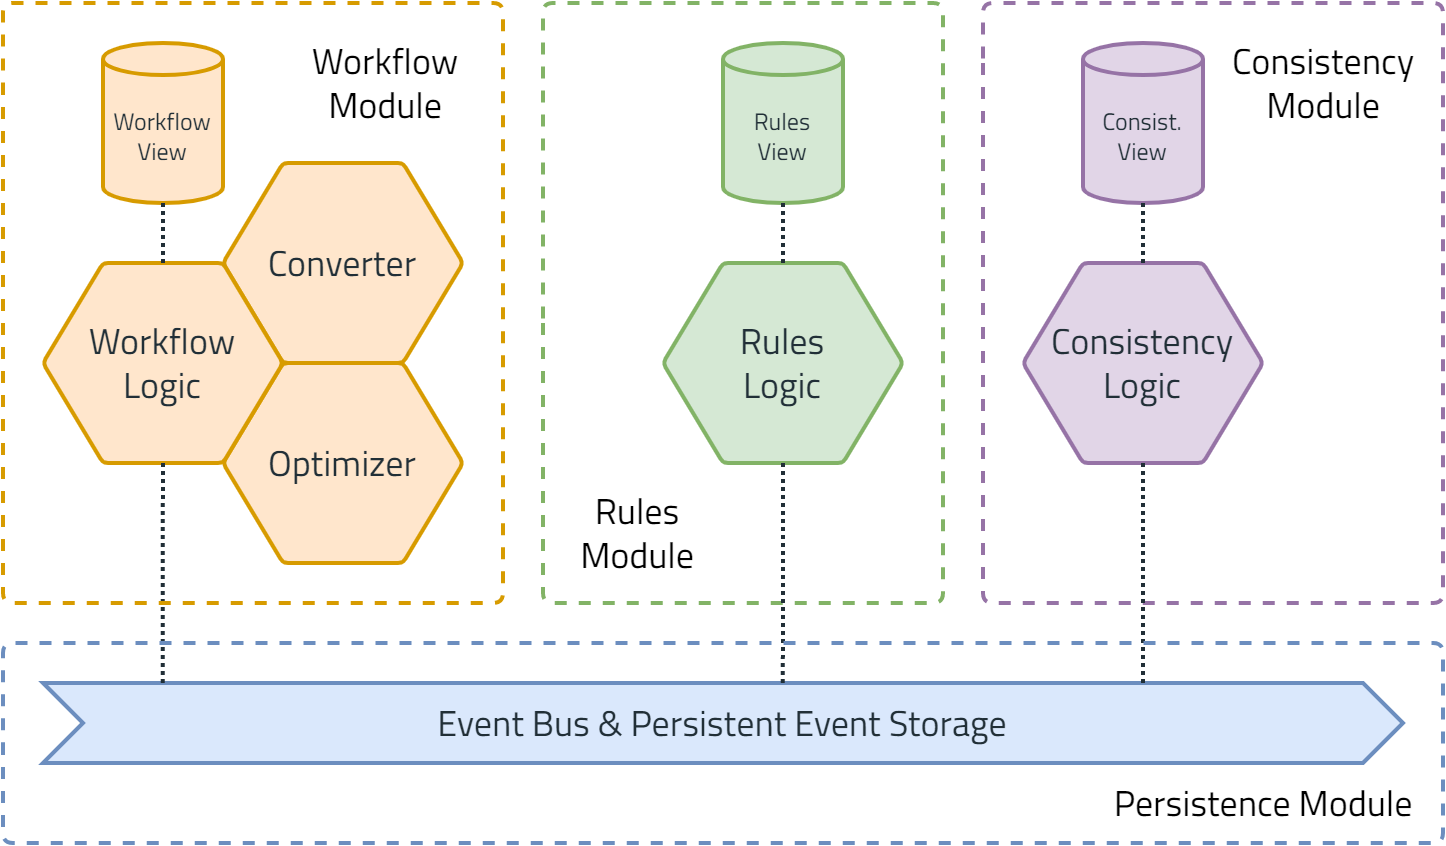
\includegraphics[width=.9\textwidth]{proposed-concept/graphics/TTSM-modules-simplified.drawio.png}}
    \caption{Macro architecture and event store design of a \gls{ttsm}.}
    \label{fig:ttsm:proposal:macro_architecture}
\end{figure}

In this software architecture, modules only communicate with each other over the event bus using predefined interfaces. It not only tries to provide a clear separation of concerns but also aims to keep stuff that changes together in close proximity to each other to improve maintainability and overall system stability. Larry Constantine, a US software engineer, shaped Constantines law, being that:

\begin{quote}
    ``A structure is stable if cohesion is high, and coupling is low.''~\cite[p.~16]{newman2019_monolith_to_microservices_constantines_law}
\end{quote}

To better illustrate the proposed concept, the remainder of this section follows along the life cycle of a single command. Commands include the creation of workflow definitions, the instantiation of workflows, and state transitions. Figure~\ref{fig:ttsm:proposal:command_life_cycle} outlines the steps that each \gls{ttsm} command has to successfully pass before consensus between participants can be reached, starting with the syntax and semantic check.

\begin{figure}[h]
    \makebox[\textwidth][c]{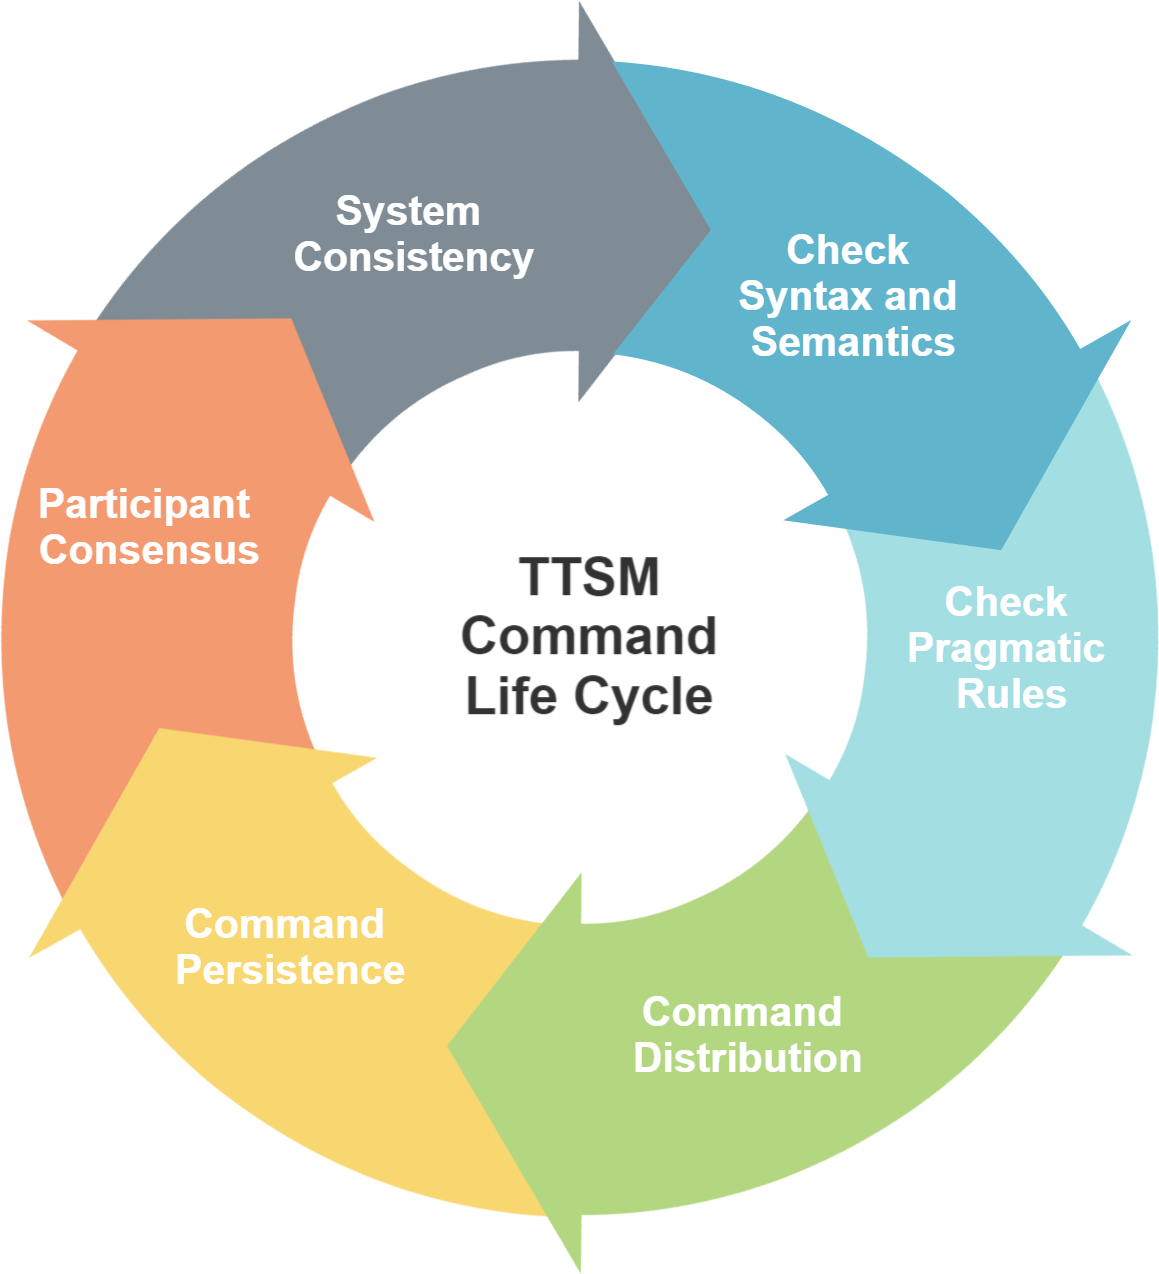
\includegraphics[width=.5\textwidth]{proposed-concept/graphics/TTSM-command-life-cycle.png}}
    \caption{Life cycle of a command dispatched in a \gls{ttsm}.}
    \label{fig:ttsm:proposal:command_life_cycle}
\end{figure}

Similar to figure~\ref{fig:ttsm:proposal:command_life_cycle}, the upcoming subsections begin with the conversion of business processes to statecharts and a check for syntactic and semantic correctness of a command. Afterwards, the rules module verifies if the command passes the employed pragmatic rules. This is followed by the distribution and persistence of the command in each participant's \gls{ttsm}. Eventually, when all participants checked and accepted the command, consensus is reached, and the system devolves into a consistent state. Note that the command life cycle is similar to the data flow in a \gls{ttsm}, where a command starts at the workflow module, passes through the rules module, and eventually reaches the consistency module. All while leaving its footprints (in the form of events) on the event bus inside the persistence module with each step. If module internal processes of defining new workflows, instantiating workflows, or performing state transitions diverge from the presented life cycle, this is stated explicitly.


%% Sender: Workflow Module
\subsection{From workflow models to statecharts}
\label{sec:ttsm:proposal:from_workflow_models_to_statecharts}
Once the participant's chosen command arrives at the workflow module, it must be converted into a statecharts-compliant format. Statecharts are used as the \glspl{ttsm} internal representation of workflows due to a vast amount of advantages, compared to \glspl{fsm}, for example, regarding workflow execution. This not only includes extensions for concurrency\footnote{An essential property for workflow execution because activities can be performed in parallel or even non-deterministic.}, but also communication between multiple participants using events~\cite{harel1987_statecharts}. Furthermore, statecharts are standardized in~\cite{statecharts_spec}, which allows developers to create appropriate tooling\footnote{e.g.,\ \url{https://xstate.js.org/} (accessed on 2022-08-15)} and the formal definition makes composition, optimization, and evaluation of statecharts more precise~\cite{inter_organizational_bps_managed_by_blockchain}. Additionally, transformation algorithms from UML sequence diagrams to statecharts~\cite{sequence_diagrams_to_statecharts} and from process models to statecharts~\cite{inter_organizational_bps_managed_by_blockchain} have been proven viable. Given the concurrency properties of statecharts, even \gls{bpmn} and choreography diagrams can be converted; however, a proof of semantic completeness for these transformations is still outstanding. Given the capabilities of statecharts and the abstraction that this transformation provides, a magnitude of modeling languages can potentially be integrated into a \gls{ttsm}. For simplicity reasons, and due to the complexity of such transformations, the remainder of this work (including the prototypical implementation in section~\ref{sec:ttsm:prototype}) assumes that participants only input statecharts compliant workflows and state\footnote{Extensions for other formats (like \gls{bpmn}) are highly encouraged to be part of future work.}.

After the transformation, the resulting statecharts are fed into the optimizer. Given a list of optimization algorithms, the \gls{ttsm} must guarantee that the specified algorithms are executed in order. A simple example of how this could be achieved is given in algorithm~\ref{alg:ttsm:proposal:ordering_optimizers}.

\begin{algorithm}
\caption{Ensure optimization algorithm order}
\label{alg:ttsm:proposal:ordering_optimizers}
\KwIn{An un-optimized statechart $s$, and a list of optimization algorithms $O$}
\KwOut{Optimized statechart $s^{\prime}$}
$s^{\prime} \gets s$\;
\ForAll{$o \in O$}
{
    $s^{\prime} \gets o(s^{\prime})$\;
}
\Return{$s^{\prime}$\;}
\end{algorithm}

Optimizers that ignore the given order can cause undesirable side effects because optimization algorithms have no means of being commutative\footnote{i.e.,\ $o_1 \circ o_2 \neq o_2 \circ o_1$}. The optimizer only runs once per workflow definition and always returns valid statecharts. There is no limitation to the amount of optimization performed; however, the semantics of the output $s^{\prime}$ should always be the same as the semantics of the input $s$. An example of such an optimization algorithm was published by Nakamura et al.~\cite{inter_organizational_bps_managed_by_blockchain} (see related work section~\ref{sec:related-work:nakamura}). Eventually, the optimization step aims to reduce the number of events emitted to the blockchain to reduce overall cost. Optimization algorithms themselves, however, are out of scope of this work. Figure~\ref{fig:ttsm:proposal:create_workflow} shows the described data and process flow inside the workflow module as sequence diagram.

\begin{figure}[h]
    \makebox[\textwidth][c]{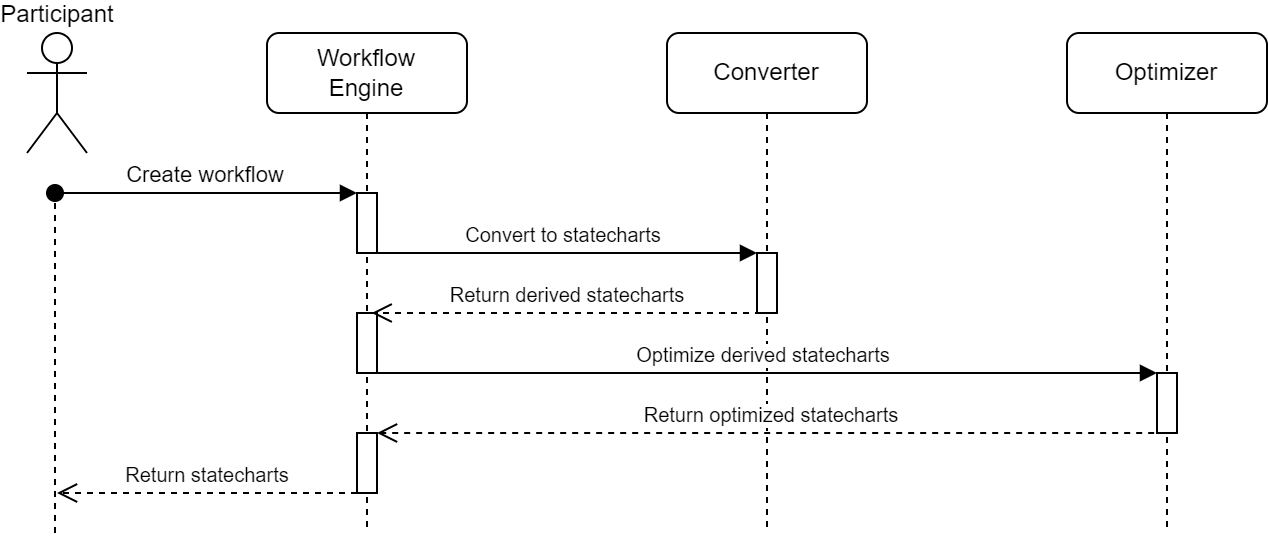
\includegraphics[width=1\textwidth]{proposed-concept/graphics/create-workflow.drawio.png}}
    \caption{Sequence diagram for the creation of a workflow definition inside the workflow module.}
    \label{fig:ttsm:proposal:create_workflow}
\end{figure}

Once optimization is complete, the workflow module checks if the given statecharts configuration is valid. Similar semantic checks are employed for workflow instantiations as well as state transitions because the state of the entire system and all workflows are known at any time and exposed by the persistence module. If the command is not allowed in the current state of the system or the workflow, it is rejected. Otherwise, it is forwarded to the event bus.


\subsection{Distinction of workflows and instantiations}
\label{sec:ttsm:proposal:distinction_workflows_instantiations}
As depicted in figure~\ref{fig:ttsm:proposal:macro_architecture}, a \gls{ttsm} is separated into four distinct modules. Clients, to be more precise \textit{workflow participants}, solely interact with the system by talking to the exposed API of the workflow module. This intended abstraction aims to hide implementation details such as the used blockchain in the consistency module or the attached rule services in the rules module. A \gls{ttsm} workflow module exposes three fundamental commands that participants can trigger at any point in time: (1) participants can propose an entirely new workflow definition with new activities and interactions between participants in the case of a choreography, (2) they can launch a new instance of a previously defined workflow definition and (3) they can initiate a state transition on a previously launched workflow instance. The separation of workflow definitions and workflow instantiations allows the association of data to a specific instantiation and thus improves flexibility~\cite{weske2012_bpm_architectures}. This is similar behavior to a lot of artifact-centric approaches such as the ones proposed by Ladleif et al.~\cite{modeling_blockchain_based_choreographies} or Lichtenstein et al.~\cite{data_driven_choreography_data_reusability_lichtenstein}. Furthermore, the separation of workflow definitions and instantiations has been shown to be rather advantageous compared to other approaches in interpreted \gls{bct}-based workflow execution engines due to the smaller footprint left behind on the blockchain itself~\cite{lean_architecture_for_blockchain_based_process_execution,interpreted_bp_on_blockchain_weber,interpreted_bp_on_blockchain_loukil}.


%% Sender: Persistence Module
\subsection{Persisting system state}
\label{sec:ttsm:proposal:capturing_local_progress}
After the successfully converted and optimized statecharts have been returned to the user for further insight, a single event is dispatched for each action to be performed (defining a new workflow, instantiating a previously defined workflow, and performing state transitions on a workflow instance) to the persistence module. The persistence module stores the entire state transition event, including its payload if present, without further processing. Technically, this allows participants to implement and add custom storage solutions without having to modifying the \gls{ttsm} itself. For large payloads, for example, state transition events may only want to reference hashes to more domain-specific databases\footnote{Such as \href{https://speckle.systems/}{Speckle} for \gls{bim} data or the \gls{ipfs}~\cite{interplanetary_file_system} as content-addressable storage (links accessed on 2022-08-21)}~\cite{weber2019_architecture_for_dapps_blockchain_patterns,eberhardt17off_block}.

Storing state transition events (and commands in general) persistently is of utmost importance for a \gls{ttsm}. All kinds of events dispatched in the system represent a delta $\Delta$ (or difference) that advances a particular workflow state and, therefore, the overall system state\footnote{Imagine a counter that adds one to the current value each time the user presses a button. In this scenario, $+1$ is the $\Delta$ to the current state, which in this case, is a counter $c$ that is initialized with $0$.}. Besides \textit{delta events}, there also exist \textit{fact events} that tell the system in which state a particular sub-state has been at a certain point in time. Unlike \textit{delta events}, \textit{fact events} are not used in \glspl{ttsm} because they can only be undone by entirely deleting them. On the other hand, when using \textit{delta events}, one can define an inverse operation\footnote{Recall the counter example from before. The inversion of the $+1 \Delta$ would be the $-1 \Delta$.}, which allows jumping forwards and backwards in time without modifying the event log itself. Therefore, the sum of commands (including state transitions or workflow instantiations) represents the current state of the system~\cite{fact_vs_delta_event_types,event_sourcing_and_cqrs}.

So-called event-driven software architectures not only allow time travel but also promote loosely coupled sub-systems and enable even better scalability. In other words, dispatched events do not require to be captured and processed by anyone. This allows modules to write events on a more fine-grained level and only consume data that is required. Additionally, due to the already employed event bus system, event sourcing can be used effectively and efficiently to create projections from the stored events and thus derive not only workflow critical information (such as the current state of a workflow instance) but also meta-data around the execution of workflows and the \gls{ttsm} itself. Furthermore, the event bus allows \glspl{ttsm} to be split into multiple microservices\footnote{One microservice per module.} if necessary. Not only can this improve scalability and availability, but also maintainability of the entire system dramatically~\cite{event_sourcing_and_cqrs}.

Due to the already employed event bus, a \gls{ttsm} aims to strictly separate between actions that modify the state and actions that solely accumulate and read the state to improve security and flexibility. Therefore, the persistence module embraces the \gls{cqrs}\footnote{\url{https://en.wikipedia.org/wiki/Command-query_separation} (accessed on 2022-08-21)} pattern as one of its design principles. At its core, \gls{cqrs} aims to separate database reads from database writes (i.e.,\ a question should not alter the state of the system)~\cite{meyer1988_effeil_and_cqs}. Separating reads from writes further improves scalability because each state transition allows an arbitrary payload with an arbitrary data structure to be attached. This means that the output of the event sourcing stage (i.e.,\ the current or any past state of a workflow instance or the system itself) can permanently be stored using a suitable database technology that is optimized for reads, for example. Event sourcing, combined with \gls{cqrs}, furthermore enables asynchronous communication with external services. To put this into the perspective of a \gls{ttsm}, participants can advance the state independently from a blockchain's required block transaction time (which can be up to 20 minutes on some blockchains~\cite{nakamoto2009}). Nonetheless, the system must expect rollbacks if workflow instances are advanced without confirmation from the rules or consistency module.


%% Sender: Time-Travelling
\subsection{Travelling through time}
\label{sec:ttsm:proposal:travelling_through_time}
The persistence module is the part of the system that enables time-travelling due to its event sourcing and \gls{cqrs} capabilities. If participants want to check if a specific event occurred or a workflow instance has fulfilled a particular property, all they have to do is (a) either search for this specific event by traversing all dispatched events forwards or backwards or (b) replay all previously dispatched events until a certain point in time is reached. The following exemplary list of events is used to better visualize this concept:

\begin{enumerate}
    \item[\textbf{E1}] \textbf{(12:00)} -- Create workflow $W$
    \item[\textbf{E2}] \textbf{(12:10)} -- Create workflow instance $I$ of workflow $W$
    \item[\textbf{E3}] \textbf{(12:20)} -- Perform state transition from state $A$ to state $B$ on $I$
    \item[\textbf{E4}] \textbf{(12:30)} -- Perform state transition from state $B$ to state $C$ on $I$
\end{enumerate}

If participants want to know, what the state of workflow instance $I$ was at 12:25, they have to replay all events that happened before or precisely at 12:25 in the correct order. Given the example above, this includes E1, E2, and E3. If participants want to know if a state transition from state $A$ to state $B$ happened prior to the state transition from state $B$ to state $C$, they have to go back in time and check if they can find appropriate events in the expected order (i.e.,\ E3 has to have happened before E4).

To allow these kinds of time-travelling capabilities, the \gls{ttsm} and the persistence module have to ensure \textit{causal ordering} for all events dispatched. This means that some event $A$ has to happen before another event $B$ can even occur - they are \textit{causally ordered}~\cite{causal_ordering}. In the example given above, event E2 can only occur after event E1 has occurred because the creation of a workflow instance requires a workflow to exist in the first place, and thus, they are \textit{causally linked}. A formal representation of this circumstance is given in equation~\ref{eq:ttsm:proposal:causal_order}.

\begin{equation}
\label{eq:ttsm:proposal:causal_order}
A \longrightarrow B
\end{equation}

Since \glspl{ttsm} ensure \textit{causal ordering}, reliable transitive relations can be derived. The persistence module knows that certain events must occur before others. An example of such a transitive relation of events is given in equation~\ref{eq:ttsm:proposal:transitive_relation}:

\begin{equation}
\label{eq:ttsm:proposal:transitive_relation}
(A \longrightarrow B \wedge B \longrightarrow C) \implies A \longrightarrow C
\end{equation}

Hence, one can express the transitive relation of events in a \gls{ttsm} as a relation $T$ over the set of events $E$ in first-order logic as follows:

\begin{equation}
\label{eq:ttsm:proposal:transitive_relation_over_ttsm_events}
\forall a, b, c \in E : (aTb \wedge bTc) \implies aTc
\end{equation}

This is an assumption that the \gls{ttsm} concept and its corresponding persistence module rely upon that allows consistent replaying of events, enhanced rule checking, and more in-depth optimizations before and during workflow execution.


%% Sender: Rules Module
\subsection{Validating workflow rules}
\label{sec:ttsm:proposal:validating_workflow_rules}
After the persistence module has eventually stored the events, the rules module consumes them. As mentioned above, this module enables participants to create supplementary and often more pragmatic rules for the entire workflow. In other words, when the workflow module checks if state transitions can be performed based on given statecharts, the rules module checks if state transitions can be performed based on previous state transitions and payloads attached. Since the rules module can directly communicate with the persistence module, it can also time-travel and check, for example, if certain state transitions have been performed or if the payload, which was previously attached to one of the state transitions, fulfills certain criteria\footnote{Specifying these criteria is up to the participants themselves, because they are very much domain specific.}.

As depicted in figure~\ref{fig:ttsm:proposal:macro_architecture}, the rules module communicates with external rule engines via a predefined interface. This interface allows the registration of rule engines that are triggered as soon as the participant proposes a new workflow definition, workflow instance, or state transition. The rules defined by the rule engines must all be unconditionally \textit{true}. If one or more rules cannot be checked due to unexpected circumstances (e.g.,\ a network timeout or the rule check returns an incomprehensible result), the rule check is evaluated to \textit{false}. A more formal representation can be found in equation~\ref{eq:ttsm:proposal:rules_module_success_criteria}. If the set of registered rule engines $R$ is empty, the \textit{rules valid} function $RV(t)$ is immediately evaluated to \textit{true}:

\begin{equation}
\label{eq:ttsm:proposal:rules_module_success_criteria}
RV(t) = \top \wedge \bigwedge_{r \in R} check(r,t)
\end{equation}

Each successful, failed, or erroneous response of $check(r,t)$ is re-emitted to the persistence module as a new event to allow for better traceability. This allows the executing participant to better trace configuration or network errors if, for example, one registered rule engine always fails for one specific state transition. After a response has been received from all registered rule engines, another event has to be emitted, which is created by the rules module, to indicate that the action to be performed is indeed allowed according to all previously defined rules. An exemplary algorithm for checking a state transition is provided in~\ref{alg:ttsm:proposal:rules_checking}.

\begin{algorithm}
\caption{Rules checking algorithm}
\label{alg:ttsm:proposal:rules_checking}
\KwIn{A state transition $t$, and an unordered set of registered rule engines $RE$}
$a \gets \top$\;
\ForAll{$re \in RE$}
{
    $v \gets check(re, t)$\;
    \eIf{$v$ is valid}
    {
        $emit(valid(re, v, t))$\;
    }
    {
        $a \gets \bot$\;
        $emit(invalid(re, v, t))$\;
    }
}
\eIf{$a = \top$}
{
    $emit(all\_valid())$\;
}
{
    $emit(some\_invalid())$\;
}
\end{algorithm}

In this algorithm, the variable $a$ is used as a tracking variable to flag if at least one rule check failed. If this is the case, the function $emit$ writes the event $some\_invalid$ to the persistence module to inform other modules of the failed rule check and allow better traceability later on. Compared to the optimizer, which is part of the workflow module, the rules module does not have to ensure ordering. This is because the overall validity check of a state transition shown in equation~\ref{eq:ttsm:proposal:rules_module_success_criteria} is commutative due to the properties of the \textit{logical and} ($\wedge$) operator.

Building upon the definition of the rules module, the number of events emitted per action can be computed using the total amount of rule engines registered $|RE|$. Each rule engine produces exactly one event, and an additional event is dispatched by the rules module after all rule checks have been performed. This circumstance is depicted in equation~\ref{eq:ttsm:proposal:number_of_rl_tx_per_action}:

\begin{equation}
\label{eq:ttsm:proposal:number_of_rl_tx_per_action}
EC_{rl}(RE) = |RE| + 1
\end{equation}


%% Sender: Consistency Module
\subsection{Sending workflow commands and ensuring consistency}
\label{sec:ttsm:proposal:entering_blockchain_and_distributing_commands}
Once the rules have been checked and the appropriate events dispatched, the consistency module consumes these follow-up events. In a \gls{ttsm} without a rules module (technically possible due to loose coupling), the consistency module might directly consume workflow events. One of the requirements that a consistency module in a \gls{ttsm} has to fulfill is multi-chain support because of the rapidly changing ecosystem of \glspl{bct}. Therefore, it has to provide some abstraction that allows the usage of different consistency strategies. In a \gls{ttsm}, this might be achieved by relying on the behavioral \textit{strategy design pattern}. This pattern allows the exchange of an algorithm during run-time without changing the interface~\cite{geirhos2015_design_patterns_behavioral}.

Combined with the approach proposed by Nakamura et al.\ in~\cite{inter_organizational_bps_managed_by_blockchain}, where a shared state machine and one for each participant are derived from a given workflow definition, and the approach proposed by Ladleif et al.\ in~\cite{architecture_for_multi_chain_bp_ladleif} for multi-chain support in workflow engines, the consistency module enables the usage of different blockchains not only in different workflow instantiations or definitions but also depending on the payload attached to state transitions, for example. Therefore, if participants agreed upon using different blockchains for different message types prior to workflow execution, the module can choose the applicable strategy implementation during runtime. As an example, the module might rely on an Ethereum-based strategy for larger \gls{bim} models, where only the hash of the model and a signature that proves that all relevant participants have seen the model is stored on the blockchain, while it might switch to a Baseledger-based strategy if documents must be proven correct using zero-knowledge. This, however, requires participants to agree on certain \glspl{bct} for certain use cases.

If an appropriate strategy has been chosen, the consistency module dispatches the message to all participants involved in the state transition. However, all messages must have at least one participant as recipient. This ensures that the internal workflow activities of one participant are not exposed to other participants. In such a case, the consistency module might even choose a noop\footnote{no operation} strategy to immediately feed back the message to the sender to prevent any network utilization at all and, thus, ensures separation of the shared state machine from the participants one.

Even though the strategy implementations can diverge, the messages exchanged always follow a strict format which is depicted in figure~\ref{fig:ttsm:proposal:consistency_message_format}.

\begin{figure}[h]
    \makebox[\textwidth][c]{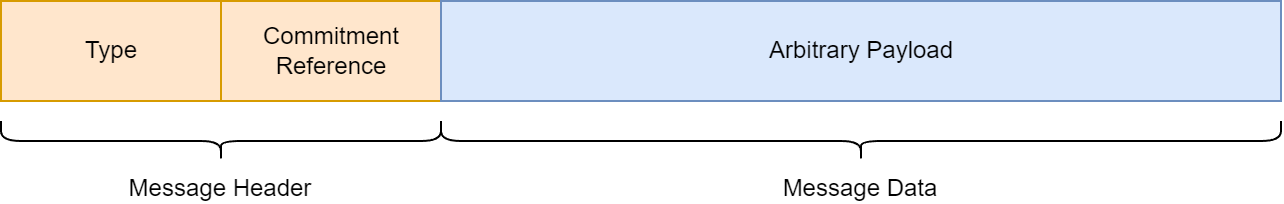
\includegraphics[width=.9\textwidth]{proposed-concept/graphics/consistency-message-format.drawio.png}}
    \caption{Format of a consistency message exchanged by participants.}
    \label{fig:ttsm:proposal:consistency_message_format}
\end{figure}

This rather simplistic configuration is split into two distinct sections: (1) the message header, which contains a unique type identifier in the form of a text string and a commitment reference that references the location where the message is stored (e.g.,\ a \gls{zkp} when using the Baseline Protocol, or a transaction reference for Ethereum or Bitcoin). (2) the message data contains an arbitrary payload using an arbitrary data structure. This might be a Base64-encoded file or even just some JSON data, for example. Depending on the message, the payload block might also contain meta information. In the case of a state transition, it stores not only the attached payload but also a unique identifier for the workflow instance on which the state transition is performed upon, the current state, the transition event name, and the expected state. Figure~\ref{fig:concept:multiple_participants} shows an exemplary setup of multiple \glspl{ttsm} to illustrate message flow between participants:

\begin{figure}[h]
    \makebox[\textwidth][c]{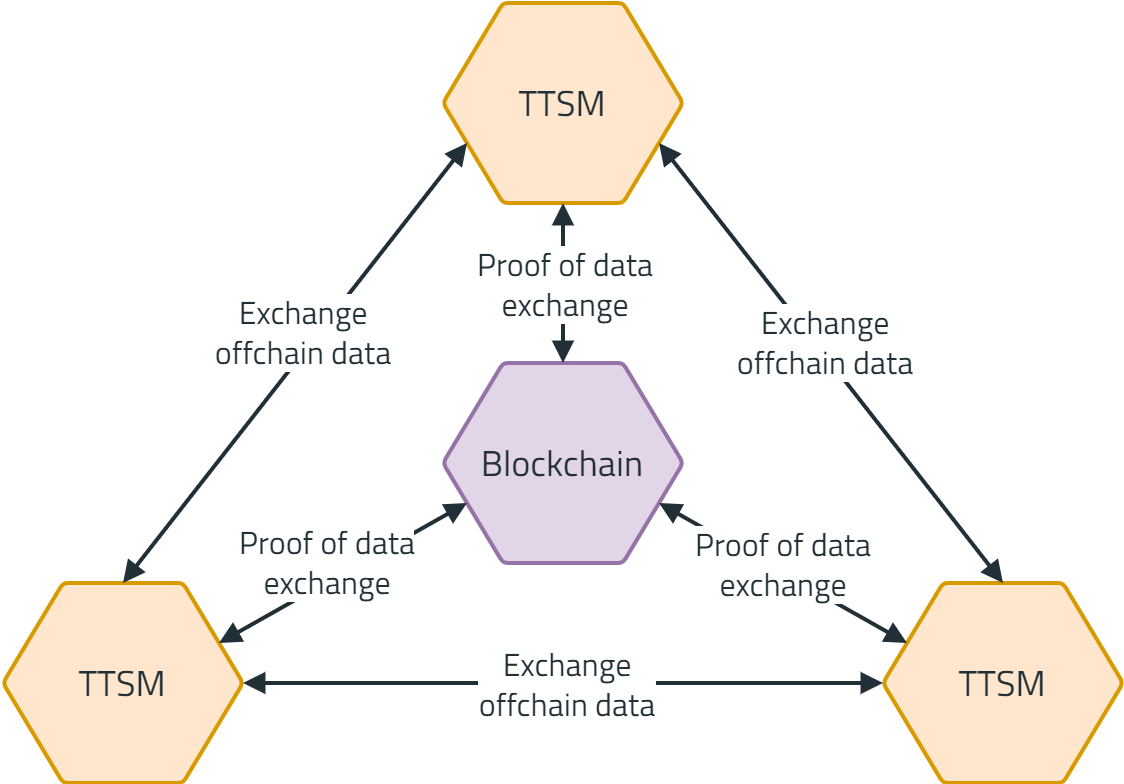
\includegraphics[width=.7\textwidth]{proposed-concept/graphics/TTSM-multiple-participants-2.drawio.png}}
    \caption{Setup of multiple \glspl{ttsm} with counterparties interacting with each other.}
    \label{fig:concept:multiple_participants}
\end{figure}

Every participant has her own instance of a \gls{ttsm}. Each \gls{ttsm} communicates with other \glspl{ttsm} by sending messages through the consistency module (by establishing TCP connections, for example). It is also the only module that directly communicates with the blockchain, in order to provide data consistency between participants.


%% Receiver: Consistency and Rules Module
\subsection{Processing workflow commands from other participants}
\label{sec:ttsm:proposal:receiving_commands}
After a connection has been established (in one way or the other, depending on the implementation of the consistency module), a message has to be dispatched to all \textit{relevant} participants of a state transition. Participants that receive this message dispatch an internal event containing the payload, the action to be performed on the workflow instance, and the commitment reference (see section~\ref{sec:ttsm:proposal:entering_blockchain_and_distributing_commands}). This ensures that all participants have undeniable proof of what happened in which order.

It is important to notice that the internal events of the \gls{ttsm} used in the persistence module are \textbf{NOT} the same events (or messages) dispatched in the consistency module and transmitted (over the blockchain) to other participants. For more complex business processes, this enables that not every single process step (including internal activities) must be written to the blockchain. This is a design constraint of the \gls{ttsm} proposal. Therefore, there can only be, at most, as many consistency events dispatched as there are persistence events. In other words, each consistency event dispatched must have at least one corresponding internal persistence event being dispatched afterwards. However, not every internal persistence event must be distributed to all other participants. This circumstance is depicted more formally in equation~\ref{eq:ttsm:proposal:comparison_bc_tx_and_events_per_transition}, where $CEC_{total}$ refers to the total number of consistency events dispatched, and $PEC_{total}$ to the total number of persistence events processed internally by the \gls{ttsm}.

\begin{equation}
\label{eq:ttsm:proposal:comparison_bc_tx_and_events_per_transition}
CEC_{total} \leq PEC_{total}
\end{equation}

After receiving the message and converting it into an internal persistence event, each \gls{ttsm} of each participant has to perform two checks:

\begin{itemize}
    \item \textbf{Syntax and semantics verification}: This check is performed by the workflow module on the transmitted data. This ensures that no incorrect state transitions, workflow definitions, or workflow instantiations can be injected by potentially hostile participants.
    \item \textbf{Rules verification}: The rules module, if present, has to perform a pragmatic verification of not only the transmitted data and its payload but also if the command is allowed in the current context regarding previously performed state transitions and their payloads. As mentioned afore, the rules module has the ability to time-travel to perform these checks.
\end{itemize}

This two-step process is the same for every command performed, even if it only regards internal workflow activities. Therefore, a participant sending a command to other participants has to perform the syntactic, semantic, and rules verification twice. Once before the consistency module transmits the command to other participants and a second time after receiving her own command. This redundant verification check ensures that commands are correctly written to the blockchain and transmitted over the network. Furthermore, it guarantees consistency because all participants work with the same commands and payloads, regardless of being sender or receiver. After verifying the command, participants generate an acceptance or rejection response. This response must be sent to all involved participants.

\begin{itemize}
    \item \textbf{Acceptance}: The participant accepts the command and advances her own \gls{ttsm} accordingly.
    \item \textbf{Rejection}: The participant rejects the command because either the syntax and semantics, the rules check, or both have failed. Denying a command restores the previous state.
\end{itemize}

If neither of both responses is sent, other participants cannot further advance their state. Handling these error cases is up to the implementation. Notice that these acceptance or rejection responses do not wait for user input. The response is entirely determined by the \gls{ttsm} internally. This means that \glspl{ttsm} do not directly support user-based decisions in workflows (e.g.,\ by asking a user in an appropriate UI if she accepts a state transition given a certain payload). However, this is entirely by design. Such user-based decisions must be modeled as part of the workflow definition itself. Statecharts, and other modeling languages that can be transformed to statecharts (such as \gls{bpmn}, for example), already include decision elements as an integral part of their specification. Therefore, user input must be handled purely declaratively on the workflow definition level by the participants themselves and is not the responsibility of the \gls{ttsm}. In other words, if a document must be shared or a decision has to be made, an applicable gateway or task must be added to the workflow.


%% Sender and Receiver: Consistency and Persistence Module
\subsection{Eventually reaching consensus}
\label{sec:ttsm:proposal:reaching_consensus}
Once a response has been sent by an involved participant\footnote{Notice that the distinction between command sender and receiver is no longer relevant at this point.}, she has to wait until all other participants have sent their responses as well. A command that concerns $N$ participants produces at most $N$ responses. At this point, the \gls{ttsm} has to handle one of three scenarios:

\begin{itemize}
    \item \textbf{Acceptance from all participants involved}: All participants accepted the command and advanced their state accordingly. Thus, consensus has been reached, and the execution of the command is complete.
    \item \textbf{Rejection from at least one participant involved}: One or more participants rejected the command and restored their previous state. Thus, all other participants must also restore their previous state to assure consistency across all parties. In other words, a rejection from at least one participant rolls back the entire command for all participants involved.
    \item \textbf{No response from at least one participant involved\footnote{See FLP impossibility result in section~\ref{sec:background:flp}.}}: This work is not concerned with this case in particular because it highly depends on implementation details and non-functional requirements such as availability, reliability, resiliency, or fault tolerance, for example.
\end{itemize}

Given these three scenarios, especially the second one is prone to attacks from hostile participants because they can deny a command infinitely many times. This threat, however, is more of a theoretical attack. Similar to the Nothing-at-Stake attack described in section~\ref{sec:background:pos}, hostile participants lose more than their potential victims. Other participants are fully aware of who rejects and who accepts commands due to the strong traceability properties of \glspl{ttsm}. Thus, the credibility of these participants suffers in the long term.

The algorithm of the consistency module, which determines the outcome of a command, is rather similar to algorithm~\ref{alg:ttsm:proposal:rules_checking} described in section~\ref{sec:ttsm:proposal:validating_workflow_rules} used to determine if a command passes the rules module. The \gls{ttsm}-consensus algorithm~\ref{alg:ttsm:proposal:consensus} is concerned with the first two scenarios described above:

\begin{algorithm}
\caption{\gls{ttsm}-consensus algorithm}
\label{alg:ttsm:proposal:consensus}
\KwIn{A command $c$, and the number of involved participants $N$}
$a \gets \top$\;
\ForAll{$i \leftarrow 1$ \KwTo $N$}
{
    $r \leftarrow next\_response()$\;
    \eIf{$r$ is acceptance}
    {
        $emit(accepted(c, r))$\;
    }
    {
        $emit(rejected(c, r))$\;
        \If{$a = \top$}
        {
            $emit(some\_rejected())$\;
        }
        $a \gets \bot$\;
    }
}
\If{$a = \top$}
{
    $emit(all\_accepted())$\;
}
\end{algorithm}

Once again, $a$ is used as a tracking variable to flag if at least one participant rejected the command. In this case, two internal events are emitted: (1) a $rejected$ event that contains not only the commitment reference but also the participant and the command itself and (2) a $some\_rejected$ event that is immediately dispatched afterwards to indicate that the command must be rolled back and the previous state restored. The algorithm, however, does not stop after one participant rejected the command. This is because all rejection responses should also be stored locally as internal events in the persistence module for better traceability.

\glspl{ttsm} leverage on the concept of ``soft state'', which means that data might be inconsistent between participants for a certain amount of time but eventually reaches consistency when things have settled~\cite{vogels2009_eventually_consistent}. This is due to the handling of participants that do not respond immediately and the block transaction time of \glspl{bct}. However, after all involved participants accepted the command, consensus has been reached and consistency archived. Therefore, the order of commands is typically determined by the consensus algorithm of the chosen \gls{bct}. Even though \glspl{ttsm} have to deal with soft state and rollbacks of commands, this single source of truth takes care of command ordering and establishing consistency between all participants.



\section{Prototype Design}
\label{sec:ttsm:prototype}
In contrast to the previous section~\ref{sec:ttsm:proposal}, this section describes a practical implementation of the proposed concept that is used for evaluation later on. Notice that not all functionalities that are theoretically possible in a \gls{ttsm} are implemented to their full extent in this prototype because it only serves as proof of concept. The prototype described uses state-of-the-art technologies and well-established industry standards to show that it is possible to implement a fully functional \gls{ttsm} leveraging on existing know-how. The upcoming sections describe a potential implementation of each module of a \gls{ttsm}. This diverges from how section~\ref{sec:ttsm:proposal} described the overall concept because this section focuses more on implementation details compared to the interoperability of the individual modules. The prototype described here is available on Zenodo\footnote{\href{https://zenodo.org/badge/latestdoi/521292268}{10.5281/zenodo.7375788} (accessed on 2022-11-29)} and GitHub\footnote{\url{https://github.com/danielkleebinder/ttsm-prototype} (accessed on 2022-11-29)}. It makes use of the following technologies:

\begin{itemize}
    \item \textbf{Node.js 16.14\footnote{\url{https://nodejs.org/} (accessed on 2022-11-29)}}: A runtime for JavaScript, built on top of the V8 JavaScript engine. It is used as an execution environment for the \gls{ttsm} itself because its event-based design makes it a good fit for systems that heavily communicate asynchronously with other systems.
    \item \textbf{npm 7.8.0\footnote{\url{https://npmjs.com/} (accessed on 2022-11-29)}}: A package manager for JavaScript and Node.js that handles dependencies using a centralized registry. Furthermore, npm also supports scripting of smaller tasks and a clear distinction between dependencies required during runtime and dependencies required during development. This allows bundled artifacts to be smaller and execute faster.
    \item \textbf{TypeScript 4.7.4\footnote{\url{https://typescriptlang.org/} (accessed on 2022-11-29)}}: A strongly typed programming language and superset of JavaScript developed by Microsoft. It is a well-established industry standard, and its sophisticated type system enables developers to create stable software for complex problems.
    \item \textbf{NestJS 8.4.7\footnote{\url{https://nestjs.com/} (accessed on 2022-11-29)}}: A Node.js framework that leverages on TypeScript for server-side applications that aims to be scalable and reliable. The frameworks module system allows dependencies between modules to be explicitly specified and, thus, creates a clear separation of concerns. This mechanism is heavily made use of to separate modules from each other.
    \item \textbf{XState 4.31.1\footnote{\url{https://xstate.js.org/} (accessed on 2022-11-29)}}: A popular, lightweight \gls{fsm} and statecharts library for TypeScript and JavaScript. It is used internally to represent statecharts derived from workflow definitions and to perform stateless state transitions in workflow instances. Statelessness is a much-wanted property given the time-travelling capabilities of a \gls{ttsm}.
    \item \textbf{EventStoreDB 21.6.0\footnote{\url{https://eventstore.com/} (accessed on 2022-11-29)}}: An event-based database that enables event sourcing. Event databases like these are a perfect fit for \glspl{ttsm} because they are not only scalable due to their built-in command-query separation and immutable state, but they also support time-travel based on previously dispatched events (see section~\ref{sec:ttsm:proposal:capturing_local_progress} for more details on why event sourcing and \gls{cqrs} are used as core concepts in \glspl{ttsm}).
    \item \textbf{Docker 20.10.13\footnote{\url{https://docker.com/} (accessed on 2022-11-29)}}: A software containerization technology, that allows the \gls{ttsm}-prototype to be launched on any system.
\end{itemize}

The upcoming sections describe, in detail, how these technologies are used to create a state-of-the-art \gls{ttsm}, based on the concept proposed in section~\ref{sec:ttsm:proposal}.


\subsection{Workflow Module}
\label{sec:ttsm:prototype:workflow_module}
The structure of the workflow module, and all modules in general, is determined by an internal three-layer software architecture, where (1) the \textit{presentation layer} exposes the endpoints that users interact with to dispatch commands such as creating new workflow definitions or performing state transitions on existing workflow instances. (2) The \textit{application layer} performs the systems workflow logic, such as converting \gls{bpmn} workflow definitions to statecharts or optimizing statecharts. And, (3) the \textit{data layer} which is responsible for storing all processed information in an immutable and append-only event log. Figure~\ref{fig:prototype:workflow_module_class_diagram} depicts the software architecture of the workflow module as \gls{uml} class diagram. The presentation layer involves the \textit{WorkflowEndpoints} class that uses the NestJS runtime environment to expose HTTP REST endpoints using distinct \glspl{dto}\footnote{Used to decouple the presentation from the application layer and only expose data that the API consumer requires.}, that are only available in the presentation layer itself. The application layer exposes the \textit{WorkflowService} that relies on the \textit{ConverterService} and the \textit{OptimizerService} to generate \gls{ttsm}-compliant statecharts. Finally, the data layer persists the produced internal events by directly accessing the \textit{EventStore}. Notice that the arrows are unidirectional between these three layers. This is a design decision that prevents circular dependencies and enables loose coupling.

\begin{figure}[h]
    \makebox[\textwidth][c]{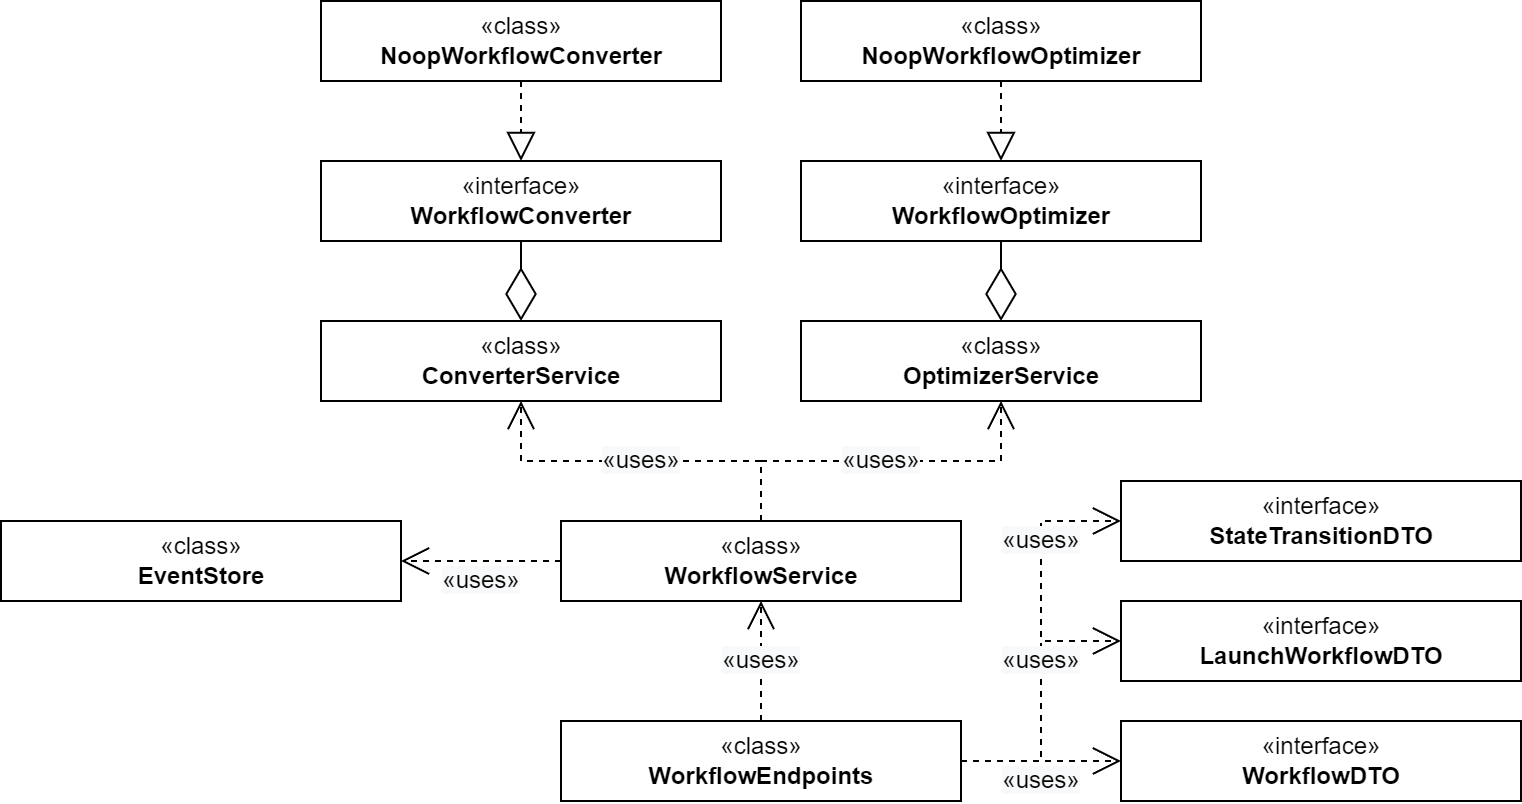
\includegraphics[width=1\textwidth]{proposed-concept/graphics/workflow-module-class-diagram.drawio.png}}
    \caption{UML class diagram of the workflow module of a prototypical \gls{ttsm}.}
    \label{fig:prototype:workflow_module_class_diagram}
\end{figure}

The \textit{WorkflowEndpoints} class also generates a fully fetched OpenAPI definition that is rendered with \textit{Redoc}\footnote{\url{https://github.com/Redocly/redoc} (accessed on 2022-10-29)}, a web-based tool, that creates beautiful single page applications that group and describe exposed endpoints in detail. Generally speaking, the \textit{WorkflowEndpoints} class receives HTTP REST commands with endpoint-specific payloads in the form of \glspl{dto}\footnote{Notice that all \glspl{dto} are marked as interfaces in figure~\ref{fig:prototype:workflow_module_class_diagram}. This is a peculiarity of the chosen programming language, TypeScript. After compiling TypeScript to JavaScript, the interfaces no longer exist because JavaScript is a dynamically typed language, and TypeScript, in contrast, is a statically typed one. Using interfaces instead of classes is, therefore, an optimization that reduces the final application size.}. These \glspl{dto} are then converted and fed forward to the \textit{WorkflowService}. Employing such a conversion allows the definition of multiple, independent endpoint classes, where each endpoint class might satisfy different specifications. This further simplifies the integration of existing solutions since the \textit{WorkflowService} class independently works with entities instead of \glspl{dto}. The endpoints exposed by the \textit{WorkflowEndpoints} class, which allow the definition of new workflows, are listed and briefly described in table~\ref{tab:ttsm:prototype:workflow_definition_endpoints}.

\begin{table}[h]
\centering
\begin{tabular}{|l|l|l|}
    \hline
    \textbf{Method} & \textbf{Path} & \textbf{Description}\\
    \hline
    POST & /workflows & Creates a new workflow and its statecharts.\\
    GET & /workflows & Returns all workflows.\\
    GET & /workflows/\{id\} & Returns the workflow with the given ID.\\
    POST & /workflows/\{id\}/launch & Launches a new instance of a workflow.\\
    \hline
\end{tabular}
\caption{List of workflow definition endpoints}
\label{tab:ttsm:prototype:workflow_definition_endpoints}
\end{table}

Based on the concept of separation between workflow definitions and workflow instantiations in section~\ref{sec:ttsm:proposal:distinction_workflows_instantiations}, workflows must be defined before they can be launched. All \textit{GET} endpoints also allow time travel by supporting an additional query parameter called \textit{until} that must be supplied with an ISO-based timestamp~\cite{iso_timestamps}. With this utility, participants can trace a workflow definition's progress, for example. Similar endpoints are exposed for workflow instantiations listed in table~\ref{tab:ttsm:prototype:workflow_instance_endpoints}.

\begin{table}[h]
\centering
\begin{tabular}{|l|l|l|}
    \hline
    \textbf{Method} & \textbf{Path} & \textbf{Description}\\
    \hline
    GET & /instances & Returns all instances.\\
    GET & /instances/\{id\} & Returns the instance with the given ID.\\
    GET & /instances/\{id\}/payloads & Returns all payloads of a particular instance.\\
    POST & /instances/\{id\}/advance & Performs a state transition.\\
    \hline
\end{tabular}
\caption{List of workflow instance endpoints}
\label{tab:ttsm:prototype:workflow_instance_endpoints}
\end{table}

After a workflow definition is launched, a workflow instantiation is created. This workflow instantiation, and its progress, can also be queried using time travel. To further advance a workflow instantiation (i.e.,\ to perform a state transition), the participant calls the \textit{advance} endpoint on the appropriate instance.

Newly created workflow definitions, instantiations, or state transitions, are then forwarded to the \textit{WorkflowService}. This service contains the actual logic of the workflow module. Since, technically, it should be possible to not only allow statecharts for workflow definitions but also \gls{bpmn} or choreography diagrams, the \textit{WorkflowService} has to choose an applicable converter. Once the workflow definition was forwarded through the \textit{WorkflowService} to the \textit{ConverterService}, the \textit{ConverterService} determines\footnote{By reading a flag that participants have to add to the workflow definition configuration.} in which format the workflow is defined and selects the correct converter strategy. The converter then outputs statecharts, where semantics are the same as the ones previously defined by the participant. Therefore, the prototype internally only ever has to work with statecharts rather than supporting a heterogeneous set of workflow definition languages. Even though it has been proven that transformations from different process definition models to statecharts are possible~\cite{sequence_diagrams_to_statecharts,inter_organizational_bps_managed_by_blockchain}, this prototype only implements the \textit{NoopWorkflowConverter} strategy that inputs statecharts and immediately, without any further transformations, outputs it. This is due to the complexity associated with converter algorithms; however, it shows the feasibility that different strategies could be supported. The algorithm for determining which converter to use is given in algorithm~\ref{alg:ttsm:prototype:choosing_converter_strategy}.

\begin{algorithm}
\caption{Choosing a converter strategy}
\label{alg:ttsm:prototype:choosing_converter_strategy}
\KwIn{A workflow definition configuration $w$, and a list of converters $C$}
\ForAll{$c \in C$}
{
    \If{$w_{type} = c_{type}$}
    {
        \Return{$c(w)$\;}
    }
}
\Return{$null$\;}
\end{algorithm}

In the algorithm implemented, $c_{type}$ represents the supported input type of the converter, and $w_{type}$ is the type specified by the participant for this particular workflow definition. After the conversion is complete, the \textit{WorkflowService} forwards the generated statecharts to the \textit{OptimizerService}. This service then picks the appropriate optimizer strategies, which are also part of the workflow definition configuration. However, compared to the \textit{ConverterService}, the \textit{OptimizerService} might not only perform a single optimization algorithm but multiple in a specified order (total ordering is guaranteed by the proposed \gls{ttsm} concept). The algorithm for this process is defined in the concept in section~\ref{sec:ttsm:proposal:from_workflow_models_to_statecharts} in algorithm~\ref{alg:ttsm:proposal:ordering_optimizers}. An exemplary definition of a simple pedestrian traffic light workflow with appropriate configuration is given in listing~\ref{lst:ttsm:prototype:pedestrian_traffic_light_config}.\\

\begin{lstlisting}[language=json,caption=Exemplary workflow definition of a pedestrian traffic light,captionpos=b,label=lst:ttsm:prototype:pedestrian_traffic_light_config]
{
  "config": {
    "optimizer": ["noop"],
    "type": "STATECHARTS"
  },
  "workflow": {
    "initial": "green",
    "states": {
      "green": { "on": { "TIMER": "red" } },
      "red": { "on": { "TIMER": "green" } }
    }
  }
}
\end{lstlisting}

The prototype only supports the \textit{NoopWorkflowOptimizer}. It immediately returns the input statecharts without modifications to show the feasibility of this multi-optimizer approach. Similar to the converter, optimizers are also rather complex and, therefore, out of scope of this work.

The generated statecharts are then fed into the \textit{XState} library to verify their syntactic and semantic validity. The library is used to depict the current state of a workflow instance and enables ``stateless'' state transitions. In the context of a \gls{ttsm}, this means that the workflow module only has to store the workflow model in the form of statecharts, as generated by the converter and the optimizer, and the current state of the workflow instance. Note that this ``statelessness'' also allows easy reconstruction of previous state machines by time-travelling and extracting the state at another point in time. If a participant wants to perform a state transition, the state machine is reconstructed by the \gls{ttsm} by feeding the workflow model and the current state into \textit{XState}. If the state transition on the reconstructed state machine fails, the workflow module responds with an error.

After conversion, optimization, and validation of workflow definitions, instantiations, and state transitions, the workflow module, and in this case the \textit{WorkflowService} in particular, dispatches a single follow-up event to the persistence module by directly connecting to the event bus of \textit{EventStoreDB}. The list of events is given below:

\begin{itemize}
    \item \textbf{Client.Workflow.Propose}: The participant wants to propose a new workflow definition for the entire network. This event includes the converted and optimized statecharts.
    \item \textbf{Client.Instance.Launch}: The participant wants to launch a new instance of a previously proposed and accepted workflow definition.
    \item \textbf{Client.Instance.Advance}: The participant wants to perform a state transition on a previously launched and accepted workflow instance.
    \item \textbf{Client.Instance.TransitionAccepted}: Some participant wants to perform a state transition, and the state machine has already incorporated it locally.
    \item \textbf{Client.Instance.TransitionFailed}: Some participant wants to perform a state transition, but the local state machine rejects it due to syntactic or semantic errors.
\end{itemize}

The connection to the event bus is also used inside the \textit{WorkflowService} to create projections of the dispatched events. These projections accumulate all events until a certain point in time (thus enabling time travel) and return the state of a particular workflow definition or instantiation.


\subsection{Persistence Module}
\label{sec:ttsm:prototype:persistence_module}
The persistence module, as mentioned afore, is an implicit module that is created by the external \textit{EventStoreDB} system. Modules that need to communicate with the event bus or the event store directly connect using the provided \textit{EventStoreDB Client}\footnote{\url{https://npmjs.com/package/@eventstore/db-client} used in version 3.4.0 (accessed on 2022-11-29)}. The client comes with full TypeScript type support and exposes a list of database command and query functions that are executed using gRPC\footnote{\url{https://grpc.io/} (accessed on 2022-09-06)}, an open source framework for remote procedure calls that is optimized for performance and throughput. To write new events to the event bus, the client provides the \textit{appendToStream} function. This function takes the name of the stream and a JSON-based payload (the event) that should be dispatched. The prototype generates an entirely new stream for each newly defined workflow definition with the name \textit{workflows.\{id\}}, to which associated events are appended. This increases performance because the overall stream size is reduced and makes reading and generating projections easier. The system does not have to filter for events with specific workflow IDs but, instead, can consume the entire stream at once. A similar mechanism has been employed for workflow instantiations. The prototype generates a new stream with the name \textit{instances.\{id\}} for each newly launched workflow instance. The IDs used for workflow definitions and instantiations are generated on the client side using UUIDv4.

Another important concept that the \gls{ttsm}-prototype heavily relies on are projections. To create projections, the \textit{EventStoreDB} client exposes the function \textit{createProjection} that inputs a unique projection name and the projection source code in the form of simplified JavaScript. Projections are typically executed for each new event dispatched to the stream it relies upon. These events are then accumulated\footnote{Imagine an event called \textit{increaseByOne} that is dispatched by some client on an irregular basis. A projection that should count the total amount would then be initialized with value $0$ and adds $1$ to the current value each time this event has been recognized.} over time and stored in a so-called \textit{materialized view}. Figure~\ref{fig:ttsm:prototype:persistence_module_architecture} shows the basic architecture and interaction between an external connector and the \textit{EventStoreDB} itself. The unidirectional arrows denote message flow direction.

\begin{figure}[h]
    \makebox[\textwidth][c]{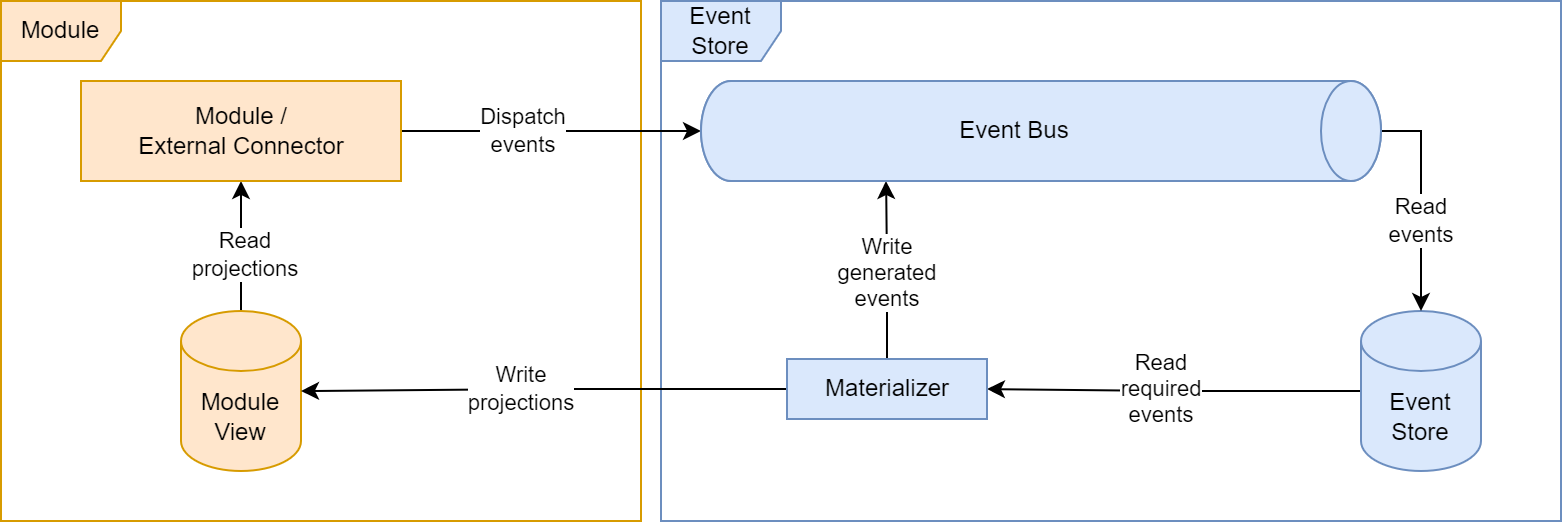
\includegraphics[width=1\textwidth]{proposed-concept/graphics/event-store-architecture.drawio.png}}
    \caption{Persistence module and event store architecture.}
    \label{fig:ttsm:prototype:persistence_module_architecture}
\end{figure}

The event store reads and persists all events dispatched to the event bus and its streams. Since projections are executed on the database side as part of the materializer, events can be directly read from the event store without any network delay involved. Therefore, this prototype could technically be scaled horizontally for large-scale systems by increasing the number of \textit{EventStoreDB} nodes. On the client side, projections generated by the materializer can be queried directly using functions like \textit{getProjectionResult} or subscribed to get notified each time the projection is updated. The second approach is typically the preferred way for event-sourcing systems because projections can be stored directly in appropriate database systems. For example, this might be a relational database system for workflow definitions or an object storage for large data sets like \gls{bim} models. For simplicity reasons, the prototype queries projection results only on demand.

In case a participant, the rules module, or any other potential client needs to verify a previous state, time travel is performed locally in the \gls{ttsm} by accumulating all events from the beginning until a given point in time. This is only possible because the \gls{ttsm} concept guarantees certain properties such as total and causal ordering of events (see section~\ref{sec:ttsm:proposal:capturing_local_progress}), or separation between the persistence of the event history and the current \gls{ttsm}-state~\cite{mistakes_in_event_sourcing}.


\subsection{Rules Module}
\label{sec:ttsm:prototype:rules_module}
This module is similar in structure to the workflow module described in section~\ref{sec:ttsm:prototype:workflow_module}. It uses a three-layer architecture, namely, presentation, application, and data layer. The presentation layer exposes the endpoints used to register external rule validation engines, the application layer performs the asynchronous validation whenever new workflow definitions, workflow instances, or state transitions are received, and the data layer, which persists validation results. These three layers are, once again, loosely coupled by the dependency injection mechanism provided by NestJS\@. Figure~\ref{fig:prototype:rules_module_class_diagram} shows the \gls{uml} class diagram of the rules module.

\begin{figure}[h]
    \makebox[\textwidth][c]{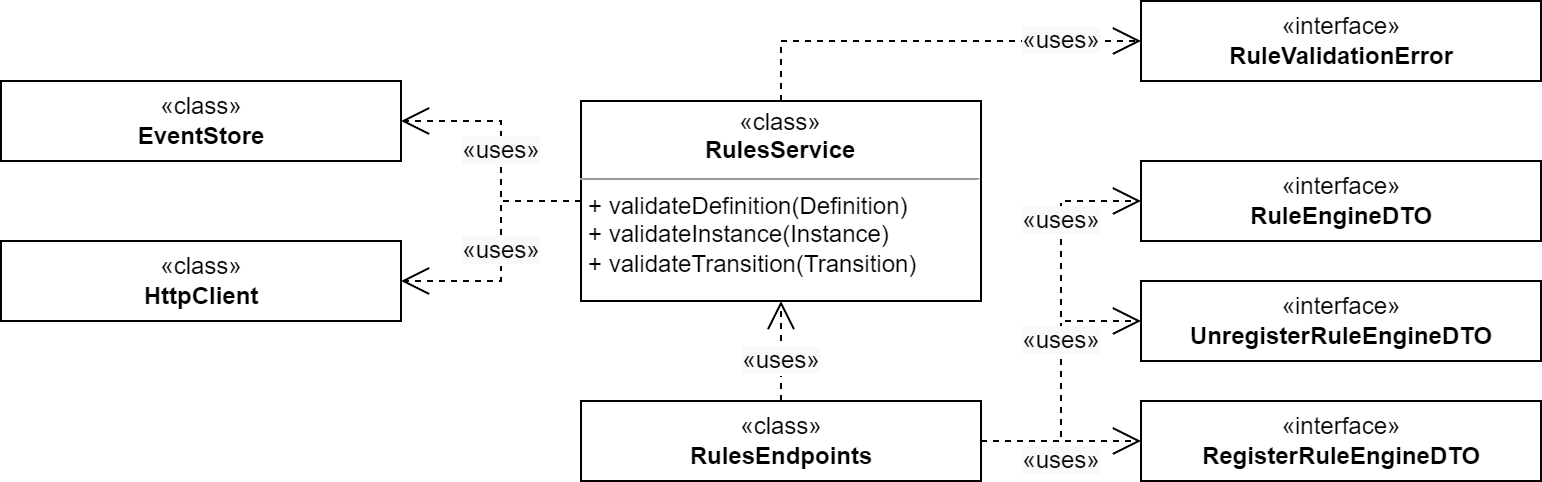
\includegraphics[width=1\textwidth]{proposed-concept/graphics/rules-module-class-diagram.drawio.png}}
    \caption{UML class diagram of the rules module of a prototypical \gls{ttsm}.}
    \label{fig:prototype:rules_module_class_diagram}
\end{figure}

The \textit{RulesEndpoints} class allows a participant that runs a particular instance of the \gls{ttsm} prototype to register rule validation engines that are later on invoked by the \textit{RulesService} if necessary. These engines are used to validate and verify if workflow definitions can be created, workflow instantiations can be launched, and state transitions can be performed under a predefined set of constraints called ``rules''. Furthermore, systems like these are technically able to connect to the persistence module directly and the endpoints exposed by the \textit{EventStoreDB} described in section~\ref{sec:ttsm:prototype:persistence_module}. This enables time-travelling capabilities inside rule validation engines. Thus, state transition and their payloads, for example, can be verified against previous state transitions and payloads\footnote{For example, a facility maintenance contractor has to complete maintenance on an elevator and transmit a document that lists all maintenance steps performed in a predefined structure and order, before the building administrator can perform an inspection. This requires semantic correctness of process execution and the rule validation engines to verify that all required documents are present in the correct form as payloads of previous state transitions.}. The implementation of such rule validation engines and how these kinds of systems let participants define rules are not part of the \gls{ttsm} itself and are out of scope of this work. Therefore, the \gls{ttsm} exposes HTTP REST endpoints that allow the registration of such systems in a loosely coupled fashion. The endpoints supported by this prototype are listed in table~\ref{tab:ttsm:prototype:rules_endpoints}.

\begin{table}[h]
\centering
\begin{tabular}{|l|l|l|}
    \hline
    \textbf{Method} & \textbf{Path} & \textbf{Description}\\
    \hline
    POST & /rules & Registers a new rule service with a callback URL.\\
    GET & /rules & Returns all registered rule services.\\
    GET & /rules/\{id\} & Returns the rule service with the given ID.\\
    PUT & /rules/\{id\} & Updates and changes details of a particular rule service.\\
    DELETE & /rules/\{id\} & Removes a particular rule service.\\
    \hline
\end{tabular}
\caption{List of rules endpoints}
\label{tab:ttsm:prototype:rules_endpoints}
\end{table}

Rule validation engines register themselves at the \gls{ttsm} with a callback URL invoked later on by the \textit{RulesService} to validate commands. The endpoints that rule validation engines must implement in order to be able to interact with the prototype properly are listed in table~\ref{tab:ttsm:prototype:rule_engine_endpoints}.

\begin{table}[h]
\centering
\begin{tabular}{|l|l|l|}
    \hline
    \textbf{Method} & \textbf{Path} & \textbf{Description}\\
    \hline
    POST & /check-new-workflow & Verifies, if the given workflow can be created.\\
    POST & /check-new-instance & Verifies, if the given instance can be launched.\\
    POST & /check-state-transition & Verifies, if the given state transition is allowed.\\
    \hline
\end{tabular}
\caption{List of required rule validation engine endpoints}
\label{tab:ttsm:prototype:rule_engine_endpoints}
\end{table}

As described in sections~\ref{sec:ttsm:proposal:validating_workflow_rules} and~\ref{sec:ttsm:proposal:receiving_commands}, there are two sources of commands that the \textit{RulesService} listens to and sends to all rule validation engines: (1) local commands, that have not yet been transmitted over the network, and (2) the commands received from other participants. In both cases, the \textit{RulesService} subscribes to the event bus of the persistence module in order to properly validate new workflow definitions, instantiations, and state transitions. The command, regardless of its source, is then sent to all rule validation engines registered. Afterwards, the \textit{RulesService} collects all responses and computes the result of the validation and verification process by algorithm~\ref{alg:ttsm:proposal:rules_checking} from section~\ref{sec:ttsm:proposal:validating_workflow_rules}. If the command has been dispatched locally and the result of the validation process is negative, it never enters the network in the first place to prevent blockchain cluttering and to keep a small footprint (see section~\ref{sec:background:on_vs_off_chain:pattern_small_footprint}). If another participant dispatches a command and the validation process is negative, the rules module creates a rejection event. A list of events that are dispatched depending on the results of the validation process is given below:

\begin{itemize}
    \item \textbf{Rules.Instance.LocalTransitionAccepted}: A local state transition has been accepted by all rule validation engines.
    \item \textbf{Rules.Instance.LocalTransitionRejected}: At least one rule validation engine has rejected a local state transition.
    \item \textbf{Rules.Instance.ReceivedTransitionAccepted}: All local rule validation engines have accepted a state transition proposed by another participant.
    \item \textbf{Rules.Instance.ReceivedTransitionRejected}: At least one local rule validation engine has rejected a state transition proposed by another participant.
\end{itemize}

Similar events are dispatched for workflow definitions and workflow instantiations. Note that, as described in the concept in section~\ref{sec:ttsm:proposal:receiving_commands}, participants that dispatch a command (like a state transition, for example) do have to validate it twice, once as a local command and the second time after receiving it through the network. This is because all commands are dispatched to all involved participants. This includes the sender of the command as well. Figure~\ref{fig:prototype:rules_module_flowchart} illustrates the decision-making process of the rules module on which event has to be dispatched as a response.

\begin{figure}[h]
    \makebox[\textwidth][c]{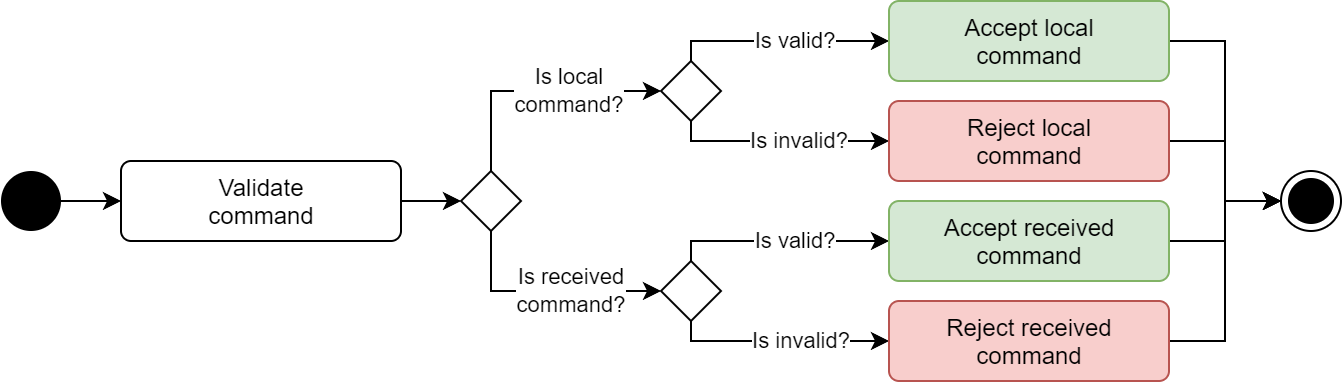
\includegraphics[width=1\textwidth]{proposed-concept/graphics/rules-module-flowchart.drawio.png}}
    \caption{UML flowchart diagram of the rules modules decision-making process.}
    \label{fig:prototype:rules_module_flowchart}
\end{figure}

Since the prototype implements the communication with rule validation engines using HTTP, unexpected network timeouts might occur. In this case, the prototype immediately rejects the command, regardless of the response of other rule validation engines, to prevent the command from being accepted that would otherwise have been rejected. This is a design decision made in the prototype since the \gls{ttsm} concept explicitly delegates the handling of network errors to the implementation (see section~\ref{sec:ttsm:proposal:reaching_consensus}). The dispatched events are then further processed by the consistency module.


\subsection{Consistency Module}
\label{sec:ttsm:prototype:consistency_module}
The consistency module, responsible for exchanging messages between participants, is implemented in this prototype using two layers: (1) the application layer being responsible for determining if a message has to be exchanged, and if so, which consistency strategy to use, and (2) the data layer that directly connects to the \textit{EventStoreDB} to listen for events triggering message exchanges. Figure~\ref{fig:ttsm:prototype:consistency_module_class_diagram} depicts the architecture of the consistency module.

\begin{figure}[h]
    \makebox[\textwidth][c]{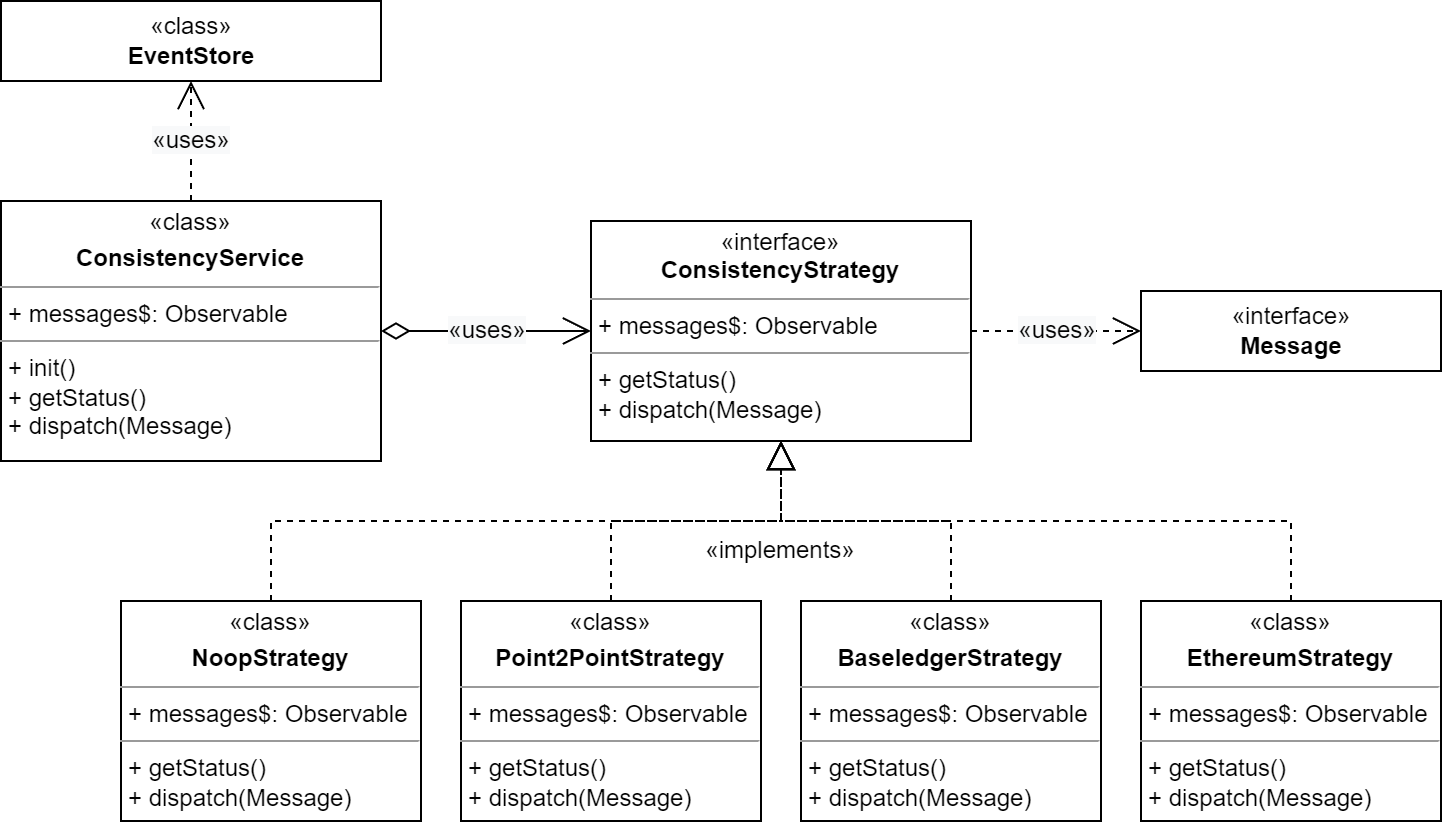
\includegraphics[width=1\textwidth]{proposed-concept/graphics/consistency-module-class-diagram.drawio.png}}
    \caption{Consistency module architecture that enables multi-chain support.}
    \label{fig:ttsm:prototype:consistency_module_class_diagram}
\end{figure}

As described in the proposed concept in section~\ref{sec:ttsm:proposal:entering_blockchain_and_distributing_commands}, the consistency module receives approval events from the rules module through the persistence module. Depending on the persistence event received, an applicable consistency message is generated. In this prototypical implementation, this is accomplished by the \textit{ConsistencyService}, which subscribes to the event bus. In a fully-fledged \gls{ttsm} implementation, the \textit{ConsistencySerivce} would now pick an appropriate \textit{ConsistencyStrategy} depending on implementation-specific metrics such as payload structure or consistency message type. However, to keep the complexity of this prototype design at a reasonable scale, the \textit{ConsistencyStrategy} that is being used is predefined on start-up by the developer. This approach might even be sufficient for most \gls{ttsm} implementations.

Consistency strategies require at least two functions and one field to be implemented. Each consistency strategy implementation has to provide the \textit{messages\$} field that implements the observer pattern and emits a new message for each message sent to other participants. It, therefore, represents a constant and congruent stream in each participant's \gls{ttsm}. The \textit{getStatus} function that returns the status of all required external services (in the case of Ethereum, for example, the status of the node used to write to the blockchain), and the \textit{dispatch(Message)} function that distributes the given message to all participants involved. Some strategies are rather specific, like the \textit{NoopStrategy}, which immediately feeds back the message to the sender (i.e.,\ it can only be used for consistency messages that involve exactly one participant), or the \textit{Point2PointStrategy} that uses HTTP to exchange messages with other participants. A potential use case for the latter one might be the distribution of messages between participants that are not in a conflict of interest, for example. However, most of the communication relies on \gls{bct}-based strategies. How these strategies are implemented and what properties these have to fulfill is out of scope of this work. Nonetheless, they are obligated by the \gls{ttsm} to exchange dispatched messages with other workflow participants reliably and to provide a consistent view of workflows throughout all participants. In this prototypical implementation, \gls{bct}-based strategies are primarily implemented in a rather simplistic way. % chktex 36

\begin{itemize}
    \item The \textbf{\textit{EvmStrategy}} generates a smart contract that only stores hashes of the exchanged messages and returns the transaction address as commitment reference. The messages themselves are exchanged using an HTTP-based REST API\@. It is forwarded to other participants only if the hash was written successfully to the smart contract and, depending on the execution mode, if the commitment reference was attached.
    \item The \textbf{\textit{BaseledgerStrategy}} works in a pretty similar fashion; however, most of the implementation of this strategy is part of the external \textit{baseledger proxy}\footnote{\url{https://github.com/Baseledger/baseledger-proxy} (accessed on 2022-09-07)}. Baseledger implements the Baseline Protocol. As described in section~\ref{sec:background:baseline_protocol}, baseledger uses an internal message bus (in this case NATS\footnote{\url{https://nats.io/} (accessed on 2022-09-07)}, a message bus for the edge) to exchange messages between participants. A \gls{zkp} is generated as a commitment reference and written to the blockchain, proving that the message was dispatched and distributed correctly.
\end{itemize}

Once the command that was converted to a consistency message has been distributed to all involved participants using the chosen consistency strategy, the \textit{ConsistencyService} receives the dispatched message (this includes the \textit{ConsistencyService} of the sender as well - no distinction between sender and receiver has to be made from here on out). The message is then converted from a consistency message transmitted over the network and exchanged between participants to an internal persistence event. Afterwards, the persistence event (and the associated command) is evaluated and validated by the rules and the workflow module for syntactic, semantic, and workflow-specific pragmatic correctness as mentioned in the proposed concept in section~\ref{sec:ttsm:proposal:receiving_commands}. As soon as all involved modules have given their feedback, the \textit{ConsistencyService} dispatches another event into the network that indicates that this \gls{ttsm} either accepts or rejects the command. All participants must wait until $N$ responses were dispatched into the network from $N$ involved participants. If one of these $N$ participants rejects the command, it is immediately rolled back. Figure~\ref{fig:ttsm:prototype:consistency_module_sequence_diagram} shows the simplified network communication between two participants exchanging messages using the \gls{ttsm} prototype.

\begin{figure}[h]
    \makebox[\textwidth][c]{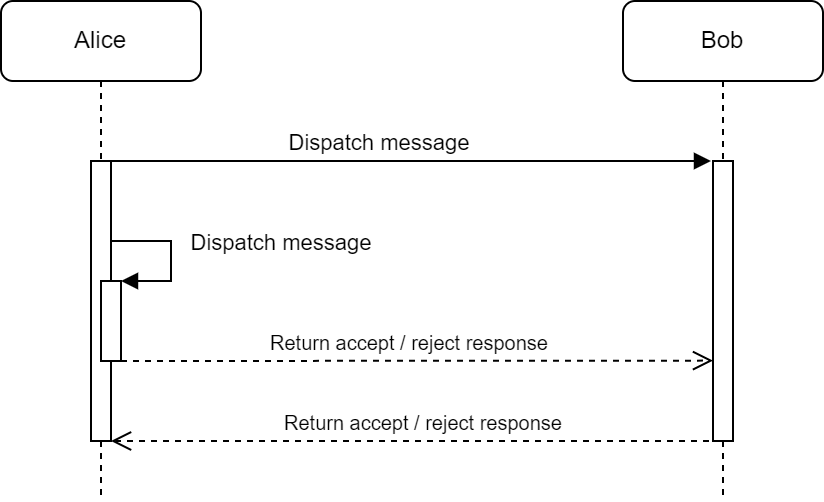
\includegraphics[width=0.8\textwidth]{proposed-concept/graphics/consistency-module-message-exchange.drawio.png}}
    \caption{Sequence diagram of two participants exchanging messages using the consistency module.}
    \label{fig:ttsm:prototype:consistency_module_sequence_diagram}
\end{figure}

The consistency messages required to perform state transitions are listed below\footnote{Similar messages are exchanged for new workflow definitions or instantiations.}. Each message, as shown in figure~\ref{fig:ttsm:proposal:consistency_message_format} in section~\ref{sec:ttsm:proposal:entering_blockchain_and_distributing_commands} consists of a message header and an arbitrary payload that is extended by message and command specific metadata.

\begin{itemize}
    \item \textbf{Perform Transition}: Some participant wants to perform a state transition on a given workflow instance. The metadata consists of the name of the state transition (unique identifier), the starting state, and the resulting state.
    \item \textbf{Accept Transition}: Response message of participants if they accept the state transition. Contains the same metadata as the \textit{perform transition} message.
    \item \textbf{Reject Transition}: Response message of participants if their workflow or rules module produced an error while evaluating the state transition. Contains the same metadata as the \textit{perform transition} message.
\end{itemize}

If an accept or reject message is received, a follow-up persistence event is dispatched by the \textit{ConsistencyService} to allow an examination of participants who rejected and accepted the command. After all responses have been collected, a completion persistence event is emitted as described in algorithm~\ref{alg:ttsm:proposal:consensus} in section~\ref{sec:ttsm:proposal:reaching_consensus}. It is used to allow the consistency module to itself determine when consensus between participants is reached. The persistence events dispatched by the \textit{ConsistencyService} are given below\footnote{Similar persistence events are dispatched for new workflow definitions or instantiations proposed by other participants.}:

\begin{itemize}
    \item \textbf{Consistency.Instance.TransitionReceived}: Created from \textit{perform transition} consistency messages and only dispatched if the workflow instance on which the transition should be performed upon and its workflow definition exist locally.
    \item \textbf{Consistency.Instance.TransitionAcceptedByParticipant}: Created from \textit{accept transition} consistency messages if any of the involved participants approve the state transition.
    \item \textbf{Consistency.Instance.TransitionRejectedByParticipant}: Created from \textit{Reject Transition} consistency messages if any of the involved participants could not perform the state transition due to some issues.
    \item \textbf{Consistency.Instance.TransitionAccepted}: Dispatched by the \textit{ConsistencyService}, if for all $N$ participants involved in the state transition, a \textit{Consistency.Instance.TransitionAcceptedByParticipant} persistence event has been dispatched.
    \item \textbf{Consistency.Instance.TransitionRejected}: Dispatched by the \textit{ConsistencyService}, if for any of the $N$ participants involved in the state transition, a \textit{Consistency.Instance.TransitionRejectedByParticipant} persistence event has been dispatched.
\end{itemize}

To dispatch persistence events, the \textit{ConsistencyService} connects to \textit{EventStoreDB} in the same fashion as the workflow and rules modules do. This includes creating projections (if necessary) and writing workflow definition events to the \textit{workflows.\{id\}} stream and workflow instance events, like state transitions, to the \textit{instances.\{id\}} stream.



\section{Intrinsic Properties}
\label{sec:ttsm:properties}
The knowledge accumulated in the background section~\ref{sec:background}, together with the research conducted to extract related work in section~\ref{sec:related-work}, led to a new concept for workflow execution that leverages on \glspl{bct} for verifiability and traceability. This concept, as described in detail in section~\ref{sec:ttsm:proposal}, and its prototypical implementation described in section~\ref{sec:ttsm:prototype} gave a sophisticated overview of properties that \glspl{ttsm} that allow time-travel verification of executed workflows need to fulfill to be viable. The following lists five distinct properties derived from the concept and the implemented prototype and describes them in more detail.

\subsubsection{Consistent}
\label{sec:ttsm:properties:consistent}
The \textit{consistency property} guarantees that all participants \textit{eventually} reach consensus and work with the exact same state for all workflows being defined or executed. As described at the beginning of section~\ref{sec:ttsm:proposal}, this property is partially enabled by the involved \glspl{bct} because their consensus protocols must guarantee at least agreement, integrity, and termination when exchanging messages and advancing the state of a blockchain (see section~\ref{sec:background:blockchain:consensus-protocols}). The \gls{ttsm}-consensus algorithm described in section~\ref{sec:ttsm:proposal:reaching_consensus} shows that the \gls{ttsm} itself can also reach consensus between all involved participants, leveraging on the aforementioned properties that \glspl{bct} and their consensus protocols bring to the table. However, due to the increased block time of certain blockchains, consistency can only be archived in the form of \textit{eventual consistency}. Nonetheless, \glspl{ttsm} that have reached finality can never be inconsistent. If participants, for example, request invalid state transitions, they are rejected immediately, which forces everyone involved to roll back. A similar scenario occurs if two or more participants aim to perform the same state transition simultaneously. Because these participants already locally advanced their state, the same transition cannot be performed twice. Even though the state transition is technically idempotent, the \gls{ttsm} still rolls back due to potentially diverging payloads. This is ensured by the workflow logic, the persistence module, and the \gls{bct} itself.

\subsubsection{Persistent}
\label{sec:ttsm:properties:persistent}
All changes performed within a \gls{ttsm} and messages exchanged between participants must be available in the form of an event history. This is referred to as the \textit{persistency property}. Persistence in the context of a \gls{ttsm} is two-fold: (1) the event bus and the event store of each participant are responsible for persisting all exchanged messages and internal \gls{ttsm} events. Since hostile participants could technically modify this data in their favor, (2) the \glspl{bct} also store certain proofs of messages that have been exchanged. Even if a hostile participant tampers their data, the other participants still have undeniable proof that specific actions have been performed. This splits persistence into two distinct areas of concern:

\begin{itemize}
    \item \textbf{Tamper-proofness}: Hinders hostile participants to change workflow execution in their favor in hindsight and generates undeniable proof (see section~\ref{sec:ttsm:proposal:entering_blockchain_and_distributing_commands}).
    \item \textbf{Storage}: Enables participants to execute large workflows with varying payloads on public blockchains without exposing privacy critical information (see section~\ref{sec:ttsm:proposal:capturing_local_progress}) and reducing the footprint on the blockchain, which reduces overall cost (see section~\ref{sec:background:on_vs_off_chain:pattern_small_footprint}).
\end{itemize}

Both properties are tightly coupled in a \gls{ttsm} to give participants access to persistence proofs on the blockchain. Due to the employed design principles of the persistence and consistency modules (such as \gls{cqrs}, event sourcing, or causal ordering), invalid commands can never become a part of the eventually consistent state of a workflow or even the entire system. Such commands are stored in the event history for traceability reasons, but are never incorporated into the state.

\subsubsection{Verifiable}
\label{sec:ttsm:properties:verifiable}
Whenever multiple participants in a conflict of interest are involved in the execution of a workflow, the \textit{verifiability property} is of utmost importance because it gives proof that certain events have happened in a particular order at a certain point in time. This property is tightly coupled with the aforementioned \textit{consistency property}~\ref{sec:ttsm:properties:consistent} and the \textit{persistency property}~\ref{sec:ttsm:properties:persistent}. Even though hostile participants might modify their local state, the global state, which is stored to some extent on the blockchain, cannot be tampered with\footnote{Given, that the underlying \gls{bct} has enough participants and implements a proper consensus protocol~\cite{public_chains_make_private_chains_obsolete}.}. If participants want to prove that some action happened in the past, they can go back in time using the time-travelling capabilities of the \gls{ttsm} and access the proof on the blockchain associated with the events. Even though not all events might be incorporated into the current system state, they are still part of the event history and hence something participants can verify. Therefore, verifiability is once again a property backed by the underlying \gls{bct} and leveraged upon in the proposed concept of a \gls{ttsm}. The consistency property ensures that the state is consistent in the first place, which guarantees that verification produces the same results for all participants, while the persistency property enables time travel which allows the verification of past states.

\subsubsection{Declarative}
\label{sec:ttsm:properties:declarative}
In order to keep development cost in case of changing requirements at a minimum, and to allow management-oriented users to define new workflows, a \gls{ttsm} has to fulfill the \textit{declarative property}. Being declarative means that users of a \gls{ttsm} can entirely configure the execution of workflows without the need for additional software development effort\footnote{An example of such a configuration is given in listing~\ref{lst:ttsm:prototype:pedestrian_traffic_light_config} in the prototype design section~\ref{sec:ttsm:prototype}.}. Being configurable and purely declarative not only enables software architects to use \glspl{ttsm} as underlying sources of truth for workflow execution, but it also simplifies the integration into existing systems. As described in sections~\ref{sec:ttsm:proposal:from_workflow_models_to_statecharts} and~\ref{sec:ttsm:prototype:workflow_module}, fully-fledged \glspl{ttsm} might not only support statecharts as the language of workflow modeling but also \gls{bpmn}, choreography or even process diagrams. Supporting well-established modeling languages further improves the practical value of such a system.

\subsubsection{Optimized}
\label{sec:ttsm:properties:optimized}
Due to highly fluctuating transaction fees of blockchains, the \gls{ttsm} should reduce the number of messages exchanged to also reduce overall cost~\cite{predicting_cryptocurrency_price_bubbles}. This is referred to as the \textit{optimization property} and is enabled by the optimizer described in section~\ref{sec:ttsm:proposal:from_workflow_models_to_statecharts} of the proposed concept. Optimizing workflow statecharts can change the syntactic meaning of workflows; however, they must preserve semantics.


\subsection{Research Question 2}
\label{sec:ttsm:properties:rq2}
To answer the second research question:

\begin{quote}
    \emph{Which properties do \gls{bct}-based state machines require to allow time-travel verification of business processes?}
\end{quote}

As mentioned above, blockchains already support a vast majority of properties required in \gls{bct}-based state machines that allow time-travel verification. However, most related work (as described in section~\ref{sec:related-work:comparison}) leverages on these properties by directly executing workflows on the blockchain. Even though tamper-proofness and consistency are assured, these approaches suffer from a lack of privacy-preserving mechanisms, longer transaction times, a lack of blockchain-acquainted developers, or restrictions to the payload size\footnote{Primarily due to native block size limits.}. Therefore, the set of properties defined for the concept proposed in this work tries to leverage on characteristics of \glspl{bct} without creating tight coupling between the blockchain and the workflow execution engine. Properties that \glspl{ttsm} \textbf{must} fulfill in order to be fully functional and to allow time-travel verification of business processes are: (1) the \textit{consistency property}, that ensures that eventually, all participants read the same state of a workflow execution, (2) the \textit{persistency property}, that stores the state in an undeniable and tamper-proof fashion without exposing privacy critical information to uninvolved participants and (3) the \textit{verifiability property}, that enables traceability through time-travel. Properties that \textbf{should} be fulfilled in order to make the concept suitable for real-world scenarios are the (1) \textit{optimization property} and (2) the \textit{declarative property}.

Nonetheless, the question remains on how the state of the art must be adapted to fulfill these properties and if integrating a \gls{ttsm} in existing systems is viable. Therefore, the upcoming sections evaluate the concept by using analytical and architectural analysis and by investigating its utility in simplified real-world scenarios.



% \subsection{Outline of the time-travelling state machine proposal}
% \begin{itemize}
    % \item Business Process / Choreography only configured via JSON or YAML (can be extended arbitrarily) to be more agnostic and keep sub-systems loosely coupled~\cite{interpreted_bp_on_blockchain_loukil}
    % \item Do not include translators because it adds complexity, gives opportunity for another master thesis and allows loose coupling
    % \item Could use state and state transition optimization as proposed by Nakamura et al. using state charts~\cite{inter_organizational_bps_managed_by_blockchain} (out of scope)
    % \item State Machine only communicates and transmits state transitions with payloads (might cause trouble with payload size in some occasions)
    % \item State Machine only writes to the blockchain, that all (relevant) parties have seen (and confirmed) the transmitted payload (2/3 of relevant participants might even be sufficient due to Byzantine fault tolerance)
    % \item State Machine internally uses \textit{Event Sourcing} to keep track of the history of state transitions but does NOT care about data transmitted
    % \item Rule Engine listens to the emitted \textit{Events} and can time-travel
    % \item All (relevant) participants must confirm that they received the business process and that they agree with the proposed state transitions (can be assumed, maybe with configuration hash, but is mostly out of scope)
    % \item Idea for Task and Business Process Design in \cite{lean_architecture_for_blockchain_based_process_execution}
    % \item Consider multi-chain support where each participant might use her own blockchain as proposed in \cite{architecture_for_multi_chain_bp_ladleif} (could be added, but out of scope)
% \end{itemize}

% \subsection{Components of a time-travelling state machine}
% \begin{itemize}
    % \item[\textbf{Consistency-Module}] Handles the communication between participants and is the only module that directly talks to the blockchain. Uses the strategy design pattern\footnote{\url{https://en.wikipedia.org/wiki/Strategy_pattern}} to integrate other forms of communication (e.g. signature-based, NOOP-strategies, smart contract strategies, etc.).
    % \item[\textbf{Persistence-Module}] Persists all events that ever occurred and exposes state for any point in time (e.g. integration of Kafka, RabbitMQ, EventSourceDB, etc.)
    % \item[\textbf{Optimizer-Module}] Optimizes communication using reduction algorithms for the configuration as mentioned here \cite{inter_organizational_bps_managed_by_blockchain}.
    % \item[\textbf{Workflow-Module}] Handles the advancement of the business process and ensures that state transitions comply with defined ``rules''. External services or sub-components could be used that make use of the time-travelling aspect of the persistence module to check if state transitions are allowed (e.g. integration of an external rule engine).
% \end{itemize}

% \subsection{Ideas during implementation}
% \begin{itemize}
    % \item All events must be idempotent because the sender will also receive all her own events (and they are now ;-)
    % \item Consistency module only depends on the persistence module and workflow module only writes into persistence module
    % \item Commitment reference is stored with every consistency event transmitted over the blockchain and is attached to events in the persistence module
    % \item Events in the persistence module are \textbf{NOT} the same as the events in the consistency module. This is due to the fact, that more complex business processes might not want to write every single process step to the blockchain because they are internal only. This surely is a design decision. Because this means, that there can only be at most as many consistency events as there are persistence events. Everything else must be dropped.
    % \item The TTSM implements the CQRS-pattern. This really helps with scalability and improves reads. Improving reads is a wanted attribute because the payload data that is transferred between states can have an arbitrary data structure depending on the use case. Allowing different database technologies for reads can improve performance dramatically (look into pros and cons of CQRS: \url{https://redhat.com/architect/pros-and-cons-cqrs}, \url{https://betterprogramming.pub/cqrs-software-architecture-pattern-the-good-the-bad-and-the-ugly-e9d6e7a34daf})
    % \item Event sourcing and CQRS allows completely asynchronous communication with external services. This means, that the client can advance the state independently from the block transaction time of the blockchain or the response of the rule engine, but has to expect rollbacks.
    % \item Depending on the proposed workflow instance, the consistency module can decide by itself which messages are being exchanged via blockchain and which blockchain strategy to use.
% \end{itemize}

% Jan Ladleif has some interesting NodeJS repositories for BPMN on his GitHub profile \url{https://github.com/jan-ladleif?tab=repositories}.



% \section{Privacy on the Blockchain}
% A lot of cool literature about zero-knowledge proofs, homomorphic encryption and TEE in \cite{blockchain_for_secure_io_bp}


\chapter{Evaluation}
\label{sec:evaluation}

\newacronym{evm}{EVM}{Ethereum Virtual Machine}

This chapter aims to thoroughly evaluate the practical feasibility of the proposed concept described in chapter~\ref{sec:ttsm}. To do so, it obeys design science guidelines and, thus, uses methodologies already available in the knowledge base of workflow execution on the blockchain~\cite{hevner2004_design_science}. This ensures better reproducibility of the presented results and allows in-depth comparison to other approaches. Two artifacts are evaluated in the following: (1) the proposed concept of a \gls{ttsm} as described in section~\ref{sec:ttsm:proposal} and (2) the instantiation of the concept in the form of the prototype described in section~\ref{sec:ttsm:prototype}. Qualitative and static analysis methodologies are applied to the former, while the latter is used for experimental analysis to show real-world utility of the proposed concept.



\section{Qualitative Analysis}
\label{sec:evaluation:qualitative_analysis}
Extracting criteria for qualitative analysis is a rather tricky task, given the heterogeneous landscape of workflow execution approaches that target the blockchain (see related work chapter~\ref{sec:related-work}). However, the most often used criteria in related literature can be categorized in flexibility and privacy or security criteria. The following list of criteria was extracted from related literature to allow comparison between different approaches. To name a few, this includes~\cite{prybila_master_thesis,runtime_verification_for_bp_utilizing_bitcoin,blockchain_for_secure_io_bp,lean_architecture_for_blockchain_based_process_execution,architecture_for_multi_chain_bp_ladleif,untrusted_bp_execution_using_blockchain}.


\subsection{Flexibility Criteria}
\label{sec:evaluation:qualitative_analysis:flexibility_criteria}
In \gls{bct}-based software, flexibility is a rare trait due to the cost associated with change on the blockchain~\cite{nakamoto2009,buterin2020}. Therefore, qualitative evaluation is performed using the upcoming flexibility criteria by creating classes ranging from low flexibility to high flexibility to put the proposed concept into perspective. Notice that higher flexibility typically comes with increased architectural complexity.

\subsubsection{Blockchain Selection}
\label{sec:evaluation:qualitative_analysis:flexibility_criteria:blockchain_selection}
For many more simple real-world scenarios, predetermining a specific blockchain to be used for the entirety of the system or particular workflow instance should be enough. However, for larger and more complex workflows, there is no singular blockchain that fulfills all necessary requirements~\cite{architecture_for_multi_chain_bp_ladleif}. Taking this into consideration, and the fact that \glspl{bct} are a rather quickly evolving sector, being able to adapt different blockchains becomes a significant point of concern for \gls{bct}-based software. Figure~\ref{fig:evaluation:qualitative_analysis:blockchain_selection_classes} shows a classification of this particular criteria.

\begin{figure}[h]
    \makebox[\textwidth][c]{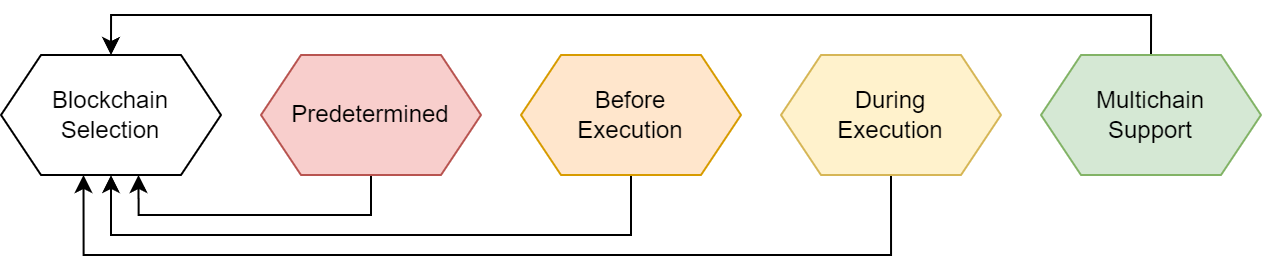
\includegraphics[width=1\textwidth]{evaluation/graphics/qualitative-analysis/blockchain-selection-classes.drawio.png}}
    \caption{A classification for blockchain selection.}
    \label{fig:evaluation:qualitative_analysis:blockchain_selection_classes}
\end{figure}

Even though there are concepts that enable multi-chain workflow execution\footnote{i.e.,\ using multiple blockchains at once that are interconnected with each other and can even exchange messages.} like the one proposed by Ladleif et al.~\cite{architecture_for_multi_chain_bp_ladleif}, most approaches rely on a single blockchain to not only execute workflows but also to tightly integrate the workflow execution system itself with the it~\cite{untrusted_bp_execution_using_blockchain,runtime_verification_for_bp_utilizing_bitcoin,bo_collaboration_between_healthcare_providers_covid_19}. The proposed concept, however, enables participants to select their preferred blockchain, and the associated desired properties, either before or dynamically during workflow execution depending on the workflow itself and the messages exchanged. This increases flexibility but also complexity due to the abstraction required.

\subsubsection{Participant Selection}
\label{sec:evaluation:qualitative_analysis:flexibility_criteria:participant_selection}
Short-running business processes and their corresponding workflows might rely on a fixed set of participants without threatening the stability or flexibility of a system or workflow. However, more volatile workflows with a considerably larger amount of participants involved need a more flexible system that enables the executing participants to select who executes certain activities on demand~\cite{fdhila2012_change_in_collaborative_processes}. Furthermore, it is advantageous for the overall workflow to select participants only after the workflow has already been launched. This allows executing participants, especially in longer-running workflows, to take environmental and political change into consideration when selecting a contractor or supplier that is required later in the workflow, for example. The classification for participant selection depicted in figure~\ref{fig:evaluation:qualitative_analysis:participant_selection_classes} differentiates between three classes ranging from least to most flexibility.

\begin{figure}[h]
    \makebox[\textwidth][c]{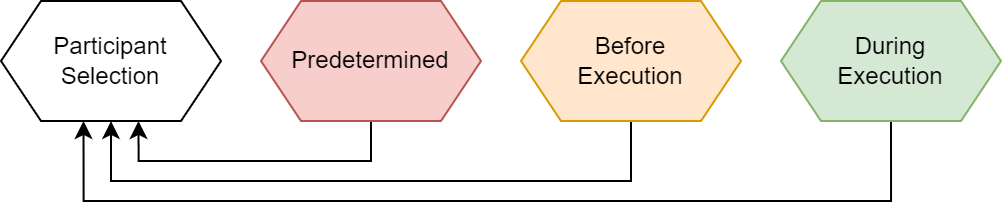
\includegraphics[width=.8\textwidth]{evaluation/graphics/qualitative-analysis/participant-selection-classes.drawio.png}}
    \caption{A classification for participant selection.}
    \label{fig:evaluation:qualitative_analysis:participant_selection_classes}
\end{figure}

Systems that predetermine all participants that are involved in the execution of workflows have not been found in related literature; however, the number of approaches that require participants to be determined before the workflow is instantiated (e.g.,\ in~\cite{modeling_blockchain_based_choreographies,inter_organizational_bps_managed_by_blockchain}), and the number of approaches that allow dynamic, or even on-demand participant selection during execution (e.g.,\ in~\cite{data_driven_choreography_data_reusability_lichtenstein,runtime_verification_for_bp_utilizing_bitcoin}), is about even. However, the concept proposed in this work does not explicitly state how participant selection should be implemented. Even though workflow definitions must specify the number of parties involved and which role they play in the overall choreography, choosing a tangible \gls{ttsm} of a participant that has been selected at a later point in time during workflow execution is still viable. This is because roles are only loosely coupled to the actual participants that carry them out. However, actions performed by participants that are no longer part of a workflow execution remain on the blockchain. This is a trait required by the persistency and verifiability properties of a \gls{ttsm} that might contradict privacy concerns to some extent\footnote{Given that no longer involved participants request data that has been associated with their participation, to be entirely removed according to the European GDPR for example.}. Nonetheless, the proposed concept technically allows any participant selection mechanism to be implemented.

\subsubsection{Workflow Mutability}
\label{sec:evaluation:qualitative_analysis:flexibility_criteria:workflow_mutability}
Being able to update workflows during execution increases flexibility even further; however, it also creates additional complexity in the form of potential issues regarding (eventual) consistency. Figure~\ref{fig:evaluation:qualitative_analysis:workflow_mutability_classes} shows a potential classification for workflow mutability.

\begin{figure}[h]
    \makebox[\textwidth][c]{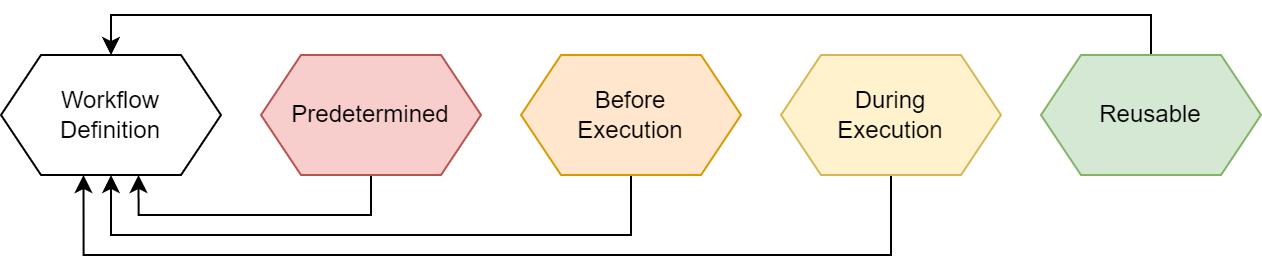
\includegraphics[width=1\textwidth]{evaluation/graphics/qualitative-analysis/workflow-mutability-classes.drawio.png}}
    \caption{A classification for workflow mutability.}
    \label{fig:evaluation:qualitative_analysis:workflow_mutability_classes}
\end{figure}

Besides predetermining workflows as part of the system being the most inflexible solution, allowing participants to define workflows themselves before execution and instantiation of the workflow itself, is the most common approach~\cite{untrusted_bp_execution_using_blockchain,bo_collaboration_between_healthcare_providers_covid_19,lean_architecture_for_blockchain_based_process_execution}. The proposed concept of this work also falls in this category performing a balancing act between complexity and reusability. Even though technically possible to adapt, allowing workflow mutability during execution or even partial reusability of already executed workflows (as described in~\cite{data_driven_choreography_data_reusability_lichtenstein}, for example) requires some changes to the concept itself. In this context, open questions like eventual consistency and participants working on different states of a workflow caused by an increased transaction inclusion duration\footnote{A commitment reference is not yet available and the command therefore not multicasted.} on certain blockchains or how to adapt reusability in \gls{bp}-centric workflow execution engines remain yet to be answered.

\subsubsection{Modelling Language}
\label{sec:evaluation:qualitative_analysis:flexibility_criteria:modelling_language}
Support for a wider range of modelling languages for workflow definitions not only improves flexibility, but also readability and reusability, because already existing process models in organizations can directly be fed into the system without the need of further adaptation. This prevents possible errors from being introduced while manually converting said models. Figure~\ref{fig:evaluation:qualitative_analysis:modelling_language_classes} includes two classifications for modelling language flexibility.

\begin{figure}[h]
    \makebox[\textwidth][c]{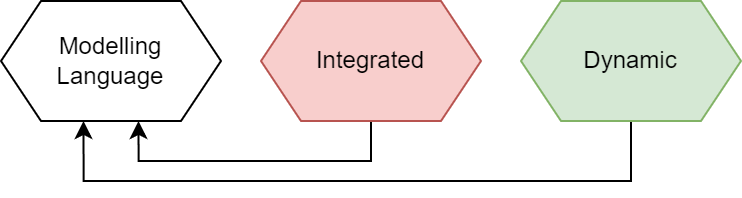
\includegraphics[width=.6\textwidth]{evaluation/graphics/qualitative-analysis/modelling-language-classes.drawio.png}}
    \caption{A classification for modelling language support.}
    \label{fig:evaluation:qualitative_analysis:modelling_language_classes}
\end{figure}

While systems, where the modelling language is tightly integrated, are strictly bound to the language semantics, dynamic approaches might require translation from one language to another. The dedicated conversion step in the workflow module (see section~\ref{sec:ttsm:proposal:from_workflow_models_to_statecharts}), puts the proposed concept on the most dynamic end of the spectrum compared to related work. Due to the internal usage of statecharts, all process models, that can be reduced to statecharts, can technically be supported. Transformations to statecharts, however, are out of scope of this work due to their complexity. Nonetheless, algorithms have been published in recent years and are publicly available for possible adaptation in a \gls{ttsm}~\cite{inter_organizational_bps_managed_by_blockchain,sequence_diagrams_to_statecharts}.


\subsection{Privacy and Security Criteria}
\label{sec:evaluation:qualitative_analysis:privacy_criteria}
Privacy is an often neglected criterion regarding workflow execution on the blockchain. In most related work, authors advise the usage of private blockchains to counteract this problem~\cite{untrusted_bp_execution_using_blockchain,bo_collaboration_between_healthcare_providers_covid_19,blockchain_based_information_sharing_in_io_workflows,lean_architecture_for_blockchain_based_process_execution,data_driven_choreography_data_reusability_lichtenstein,interpreted_bp_on_blockchain_loukil}. However, this approach only partially solves the issue, and some open problems remain. Companies might want to treat parts of internal workflows as a trade secret because they are of utmost importance to the business's success or because they are simply not relevant to the shared \gls{bp}. Another example is confidential information that is only allowed to be shared between two particular participants and must never be exposed to others\footnote{Imagine a four-party scenario where three banks and the government are involved. All participants agree on using a blockchain as a trusted third party. Some information about customers, however, is only allowed to be shared with the governmental instance and not with any other participant due to privacy regulations. Private blockchains cannot solve this issue if the privacy critical data is stored on-chain because all four participants can investigate the state of the blockchain at any point in time.}. Furthermore, the usage of private blockchains can threaten security, as previously discussed in chapter~\ref{sec:related-work}, due to the increased voting power per participant compared to public blockchains. Similar to the flexibility criteria, the upcoming privacy and security criteria are also divided into classes to put the proposed concept into perspective.

\subsubsection{Workflow Structure Sharing} \label{sec:evaluation:qualitative_analysis:privacy_criteria:workflow_structure_sharing}
Workflows that involve multiple independent participants do require sharing of workflow structures in some form to create a common frame of reference. Figure~\ref{fig:evaluation:qualitative_analysis:workflow_structure_sharing_classes} differentiates between three public and one private classification. First, public workflows that share not only their structure but also their execution context\footnote{In the form of smart contracts, for example.}. Second, public actions, where only state transitions are exposed; and third, public metadata, where only (encrypted) metadata about the workflow is shared publicly. Purely private workflows are the fourth class, in which no information is put on a blockchain that is used by more than one participant.

\begin{figure}[h]
    \makebox[\textwidth][c]{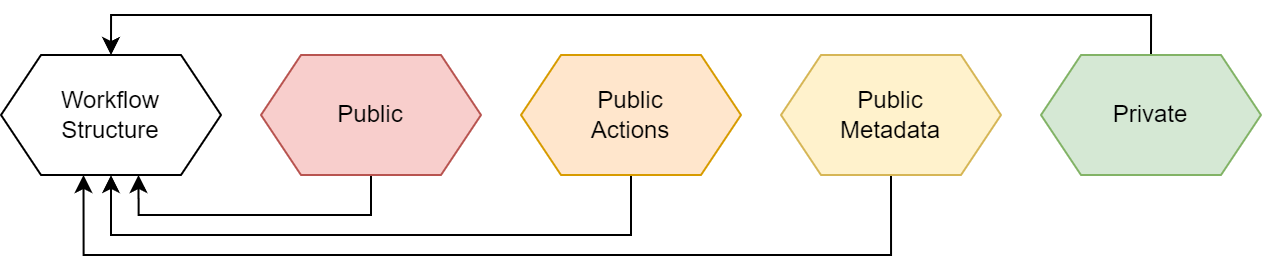
\includegraphics[width=1\textwidth]{evaluation/graphics/qualitative-analysis/workflow-structure-sharing-classes.drawio.png}}
    \caption{A classification for sharing workflow structures.}
    \label{fig:evaluation:qualitative_analysis:workflow_structure_sharing_classes}
\end{figure}

Depending on the implementation of the consistency module of a \gls{ttsm} and the chosen consistency strategy, the proposed concept might either fall into the second or third category --- sharing actions or metadata on the public blockchain, but is never executing entirely on-chain (restricted by the architecture by separating the workflow module from the consistency and persistence modules). Strategies for sharing workflow structures might include transmitting actions off-chain but storing hashes or \glspl{zkp} of actions being performed on-chain. Furthermore, the proposed concept aims to only share choreography structures that determine the required interactions between participants. Internal workflow structures can be kept entirely private or semi-private by leveraging on homomorphic encryption or \glspl{zkp}, for example.

\subsubsection{Data Sharing}
\label{sec:evaluation:qualitative_analysis:privacy_criteria:data_sharing}
The way workflow execution engines share data associated with workflows and state transitions is categorized by the classification given in figure~\ref{fig:evaluation:qualitative_analysis:data_sharing_classes}. It differentiates between data being shared over a public network and thus being available to all workflow participants, only sharing (encrypted) metadata or keeping data entirely private.

\begin{figure}[h]
    \makebox[\textwidth][c]{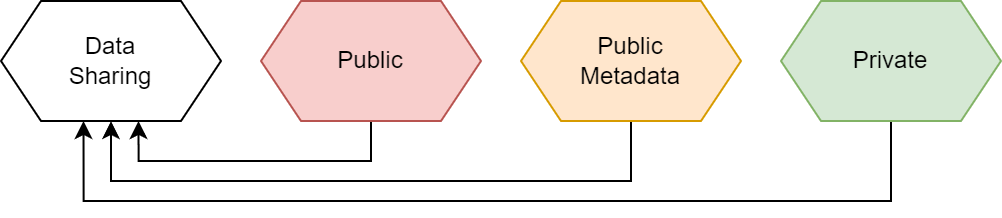
\includegraphics[width=.8\textwidth]{evaluation/graphics/qualitative-analysis/data-sharing-classes.drawio.png}}
    \caption{A classification for sharing data between participants.}
    \label{fig:evaluation:qualitative_analysis:data_sharing_classes}
\end{figure}

Most approaches found in related literature either require participants to share data entirely off-chain or entirely on-chain. The former approach neglects traceability capabilities of \glspl{bct}, and the latter restricts payload size to the maximum allowed block and transaction size of the (most often) predetermined blockchains being used. Other approaches, like the ones proposed by Lichtenstein et al.~\cite{data_driven_choreography_data_reusability_lichtenstein}, and Ladleif et al.~\cite{modeling_blockchain_based_choreographies}, which are laying their focus on the artifacts produced by workflows, also store the state and life cycle of the entire artifact on-chain and thus, makes them publicly (in the sense of ``for all participants'') available. However, the concept proposed in this work aims to bridge the gap in the related literature by only storing metadata on-chain. Similar to the workflow structures described in the previous criteria~\ref{sec:evaluation:qualitative_analysis:privacy_criteria:workflow_structure_sharing}, a \gls{ttsm} only stores hashes of actions and their associated payload data or \glspl{zkp}, for example, that ensure, that the data fulfills specific properties. Open questions, especially regarding techniques like \glspl{zkp} or homomorphic encryption, must still be solved in future work to fully leverage on the capabilities of the proposed concept.

\subsubsection{Trust}
\label{sec:evaluation:qualitative_analysis:privacy_criteria:trust}
Trust between participants is vital when they are in a conflict of interest. Studies have shown that incorporating trust as a key ingredient into workflow systems might increase workflow performance, particularly in supply chain management and logistics~\cite{fynes2005_impact_of_relationships_on_supply_chain_performance,johnston2004_supplier_trust_performance}.
A common solution to establish trust is to utilize trusted third parties~\cite{impact_of_trust_on_supply_chains,trust_in_service_oriented_ds_through_blockchain}. All approaches discussed in chapter~\ref{sec:related-work} build upon the blockchain to take up this particular role. So does the concept proposed in this work. To enable traceability through the blockchain, the consistency module of a \gls{ttsm} associates exchanged messages with commitment references. This ensures that all actions that require multi-party participation are undeniably persisted and can be verified. However, the proposed concept does not support authentication mechanisms. This means that participants occupying a particular workflow role might not be who they pretend they are. Even though workflow execution does not inflict trust-related issues, the open authentication problem might. To participate in a workflow that is handled by a \gls{bct}-based \gls{ttsm}, participants require a blockchain wallet in some form to at least provide a pseudo-identity\footnote{\glspl{bct} provide pseudo-anonymity, thus, it is practically almost impossible to authenticate a participant by her wallet information.}. However, more is needed to authenticate participants trustfully because a wallet might also belong to an attacker pretending to be a particular participant. Thus, authentication remains an open problem which is out of scope of this work due to its complexity. Future work might consider the usage of asymmetric cryptography and signatures in order to solve this issue.

\subsubsection{Conflict Resolution}
\label{sec:evaluation:qualitative_analysis:privacy_criteria:conflict_resolution}
Resolving conflicts between participants using undeniable proofs is one of the cornerstones that blockchains provide. The proposed concept leverages on this property by referencing commitments on the blockchain for each action performed by any of the participants. Therefore, conflicts can be resolved by the time-travel capabilities of a \gls{ttsm} - participants involved in a conflict can travel back in time to the point where the conflict arose. The workflow at this point in time contains all actions that led to the current state and, thus, all associated commitment references on the blockchain, which in fact, are undeniable proof of what happened\footnote{Given that the blockchain itself is tamper-proof (see consensus section~\ref{sec:background:consensus} for more details).}. Nonetheless, a follow-up issue arises regarding the authentication of participants mentioned before in criteria~\ref{sec:evaluation:qualitative_analysis:privacy_criteria:trust}. Even though a role might have performed an action according to the blockchain, this does not give proof that the action has indeed been performed by the correct participant. Due to the pseudo-anonymity of blockchains, one can not easily prove the identity of contributors without further usage of off-chain techniques such as legal contracts associating a participant to a wallet address, for example. Resolving the authentication and identity issue in future work might also solve the conflict resolution issue mentioned in this section.


\subsection{Summary and Discussion}
\label{sec:evaluation:qualitative_analysis:summary}
The qualitative analysis performed in this section has shown significant traits of the proposed concept regarding flexibility compared to existing solutions. For the most part, this can be traced back to the role of the blockchain that is only of supportive nature, a characteristic that has not been investigated in related work and \gls{bct}-based workflow execution yet. By leveraging on the blockchain without statically integrating it as a software architectural cornerstone, \glspl{ttsm} are not bound to restrictions given by the blockchain ecosystem. Compared to other concepts, this allows the concept proposed in this work to be more flexible and extensible, resulting in a highly modular architecture where components are only loosely coupled and interchangeable at any point in time. This kind of flexibility has been an unseen trait in \gls{bct}-based workflow execution engines and results in a list of advantages that are otherwise difficult to obtain, including \glspl{ttsm} switching blockchains during workflow execution without significant complexity overhead\footnote{Note that, regarding practical feasibility, participants have to determine which blockchain is best suited for which message types in order to guarantee flawless transitions during execution. Furthermore, data remains on the blockchains it was initially written to. Time travel and verification, therefore, also includes switching between blockchains.}, dynamically selecting participants on-demand, or changing the (shared or internal) workflow definition during runtime. However, two gaps in the state of the art and the proposed concept have been identified regarding blockchain interaction and authentication of participants:

\begin{itemize}
    \item Investigation of applicable techniques that store minimum amounts of data on-chain but provide maximum traceability and verifiability.
    \item Investigation of authentication techniques for blockchain participants, to prove identity (also referred to as decentralized identifiers\footnote{\url{https://w3.org/TR/did-core/} (accessed on 2022-11-29)}), to seal attack vectors like Sybil attacks.
\end{itemize}

Solving these two research problems (1) further reduces transaction cost while not endangering the traceability and verifiability that \glspl{ttsm} already provide, and (2) being able to undeniably associate actions being performed by participants with real-world identities. Nonetheless, the qualitative analysis has shown that the proposed concept combines traits from different approaches while reducing the footprint on the blockchain, preserving privacy to some extent, and improving flexibility.



\section{Static Analysis}
\label{sec:evaluation:static_analysis}
In this section, the static structure of the proposed concept is analyzed by deriving formal metrics and taking a closer look at the macro software architecture. It aims to give insight into the complexity and cost of a \gls{ttsm}. In order to do so, the remainder of this section assumes the usage of a layer-1 \gls{bct}-based consistency strategy in the consistency module to assure comparability with related work~\cite{untrusted_bp_execution_using_blockchain,interpreted_bp_on_blockchain_loukil,runtime_verification_for_bp_utilizing_bitcoin,interpreted_bp_on_blockchain_weber}. The \gls{bct}-based consistency strategy creates a peer-to-peer network where each participant is directly connected to all the other participants. An additional connection to the blockchain is established that is used to prove the integrity of each message exchanged. Other technologies, such as layer-2 rollups or using \glspl{zkp}, might yield other results.


\subsection{Network Topology}
\label{sec:evaluation:static_analysis:network_topology}
The \gls{ttsm} network topology is determined by the number of workflow participants, only including the ones that are relevant to perform a specific command. Even if the workflow requires a total of $N$ roles, certain state transitions might only interact with $n < N$ participants occupying a subset of the $N$ roles. In the following, state transitions are used exemplary for any kind of command w.l.o.g. Given a state transition that requires interaction with $n$ participants, the \textit{maximum} number of connections each participant has to establish can be derived from the fact that the \gls{ttsm} concept operates on a peer-to-peer network. Thus $n - 1$ connections must be established, excluding the participant that proposed the state transition. Therefore, the total number of connections required is equal to the number of edges in a complete graph. The computation is given in equation~\ref{eq:evaluation:static_analysis:max_number_of_connections} with $C_{max}$ being the total number of connections required. % chktex 35

\begin{equation}
\label{eq:evaluation:static_analysis:max_number_of_connections}
C_{max}(n) = \frac{n(n-1)}{2} % chktex 35
\end{equation}

The proposal of a single state transition only requires the proposing participant to connect to $n - 1$ (excluding self) involved participants. Each involved participant, excluding the proposing one, has to establish precisely one connection resulting in a total amount of $n - 1$. However, after receiving the state transition, each participant has to send an accept or reject message to all other $n - 1$ participants. Thus, resulting in a complete graph or ``fully connected mesh''. One can now derive the total number of messages exchanged $M$ when performing a state transition\footnote{Starting in the proposal phase until the transaction has been included into a block.} using equation~\ref{eq:evaluation:static_analysis:number_of_messages_per_transition}.

\begin{equation}
\label{eq:evaluation:static_analysis:number_of_messages_per_transition}
M(n) = n ^ 2 + n
\end{equation}

The number of messages per state transition is therefore quadratically bound to the number of involved participants assuming that a message is not only sent to the other $n - 1$ participants but also to one self\footnote{Imagine an exemplary scenario, where four parties are involved: (1) the product manufacturer, (2) the reseller, (3) the customs authorities and (4) the freight forwarder. When the reseller orders a product, only the reseller, and the manufacturer have to perform and accept the state transition (i.e.,\ all participants involved in an activity). Given that $N=4$ and $n=2$, the total number of messages exchanged over the network is $2^2+2=6$ and the number of connections is $\frac{2(2-1)}{2}=1$. The customs authorities and the freight forwarder may not receive any messages at all at this point.}. Expressed in Landau notation, this results in an overall communication complexity of $\mathcal{O}(n^2)$ given that $n > 1$ when performing actions w.l.o.g.


\subsection{Blockchain Transactions}
\label{sec:evaluation:static_analysis:blockchain_transactions}
Similar to the network topology, the maximum number of blockchain transactions is also determined by the number of involved participants required for a specific command. Given a total of $N$ roles and $n$ participants, launching a workflow might involve $n \geq N$ participants\footnote{A single role might be fulfilled by different participants at different points in time.}, however, performing state transitions most of the time requires $n \leq N$ participants. Thus, the maximum number of transactions on the blockchain is linear to the number of involved participants, as shown in equation~\ref{eq:evaluation:static_analysis:number_of_bc_tx_per_transition} where $TC$ is the blockchain \textit{transaction count} and $t_p$ the number of \textit{participants} involved in the command.

\begin{equation}
\label{eq:evaluation:static_analysis:number_of_bc_tx_per_transition}
TC(t) = \begin{cases}
            0 & \text{for $t_p < 1$} \\
            t_p + 1 & \text{for $t_p \geq 1$}
        \end{cases}
\end{equation}

Commands involving one participant (i.e.,\ themselves) typically do not require blockchain interaction. However, in certain scenarios, a participant might want to prove to an external party that a specific artifact existed at a particular point in time. Given that a \gls{ttsm} solely operates on statecharts, one can derive the total number of blockchain transactions per workflow instance as follows. Let $W$ be a workflow defined as statechart and formalized as 5-tuple $\langle S, s_0, F, E, T \rangle$ where S is the set of possible states, $s_0 \in S$ the initial state, $F \subseteq S$ being the set of final states and $T$ is the set of transitions. Then, the total amount of required blockchain transactions is linear to the cardinality of $T$ denoted as $|T|$ and, in case of loops or decisions in a workflow, the number of state transitions $t_c$ performed per $t \in T$ with $TC_{total}$ being the \textit{total transaction count} on the blockchain.

\begin{equation}
\label{eq:evaluation:static_analysis:total_number_of_bc_tx_per_bp}
TC_{total} = \sum_{t \in T} TC(t) \cdot t_c
\end{equation}

Equation~\ref{eq:evaluation:static_analysis:total_number_of_bc_tx_per_bp} computes the maximum number of blockchain transactions in a workflow instance as a summation of state transitions $t \in T$ and the associated number of required participants. Leveraging on the notation defined above, one can derive the average number of participants involved per state transitions $\overline{n}$ as follows.

\begin{equation}
\label{eq:evaluation:static_analysis:average_number_of_participants}
\overline{n} = \sum_{t \in T} \frac{t_p}{t_c}
\end{equation}

Given $\overline{n}$ participants that have been required to complete workflow instance $I$ on average and $m$ being the total number of state transitions performed, the overall communication complexity is linear and comes down to $\mathcal{O}(\overline{n} \cdot m)$ which simplifies to $\mathcal{O}(m)$ assuming $\overline{n}$ being the smaller factor.


\subsection{Persistence Events}
\label{sec:evaluation:static_analysis:persistence_events}
The number of persistence events dispatched by a \gls{ttsm} always has to equal or be greater than the number of blockchain transactions (see section~\ref{sec:ttsm:proposal:receiving_commands}). This is a constraint required by the persistence and verifiability properties described in section~\ref{sec:ttsm:properties} and can be formally expressed as $TC_{total} \leq EC_{total}$. To compute $EC_{total}$, one must first compute the number of persistence events per state transition. Let $T$ be the set of possible state transitions in an arbitrary statechart defined as $\langle S, s_0, F, E, T \rangle$. Then, the number of persistence events dispatched per state transition $t \in T$ is computed as follows.

\begin{equation}
\label{eq:ttsm:proposal:number_of_events_per_transition}
EC(t) = (t_p + 1) + (t_r + 1) + 1
\end{equation}

In the first step, a single participant requests a state transition. This state transition is received and persisted by all involved participants. Afterwards, the local rule system dispatches a persistence event (including the validation results) for each rule engine registered $t_r$ and one that indicates if the overall validation process was successful. In the last step, each participant has to either send an accept or reject message over the network, which results in a single persistence event per participant $t_p$. An additional event is dispatched to indicate if all involved participants accepted or at least one rejected the proposed state transition. Participants not involved in a state transition do not emit any persistence events. Therefore, the total number of persistence events $EC_{total}$ can be computed as the sum of persistence events per state transition performed.

\begin{equation}
\label{eq:ttsm:proposal:total_number_of_events_per_bp}
EC_{total} = \sum_{t \in T} EC(t) \cdot t_c
\end{equation}

One observation when comparing $EC_{total}$ to $TC_{total}$ is that $EC_{total}$ is always larger than $TC_{total}$ because, in addition to the events dispatched per participant, $EC(t)$ also includes the events dispatched by the rules module and an additional event that indicates the final status of the command.

% Similar to equation~\ref{eq:evaluation:static_analysis:total_number_of_bc_tx_per_bp}, equation~\ref{eq:ttsm:proposal:total_number_of_events_per_bp} also leverages on $t_c$ to indicate how often $t \in T$ has been performed in a workflow instance. Proving that $TC_{total} \leq EC_{total}$ holds now becomes a straightforward task by substituting for $TC_{total}$ and $EC_{total}$:

% \begin{equation}
% \sum_{t \in T} TC(t) \cdot t_c \leq \sum_{t \in T} EC(t) \cdot t_c
% \end{equation}

% It becomes clear that one is \textit{strictly larger} than the other when substituting and simplifying both functions $TC(t)$ and $EC(t)$. The lower bound $t_p \leq 1$ in $TC(t)$ is ignored because this proof is only concerned with the upper bounds of both functions:

% \begin{equation}
% \sum_{t \in T} (t_p + 1) \cdot t_c < \sum_{t \in T} (t_p + 3 + t_r) \cdot t_c
% \end{equation}

% Thus, a \gls{ttsm} always emits \textit{strictly more} persistence events than blockchain transactions required, regardless of the number of participants, resulting in $TC_{total} < EC_{total}$.

% \begin{flushright}
% $\blacksquare$
% \end{flushright}


\subsection{Summary and Discussion}
\label{sec:evaluation:static_analysis:summary}
The formal static analysis performed in this section has shown that the overall complexity of the network, required in a \gls{ttsm}, is bound quadratically to the number of participants due to the underlying ``fully connected mesh'' topology. This increases resiliency because, in theory, participants can forward messages to other participants, but it also increases the complexity of the required infrastructure. Figure~\ref{fig:evaluation:static_analysis:partially_connected_mesh} depicts a possible setup between three participants, namely Alice, Bob, and Mallory, where the direct link between Alice and Bob has been lost, and Mallory must forward messages.

\begin{figure}[h]
    \makebox[\textwidth][c]{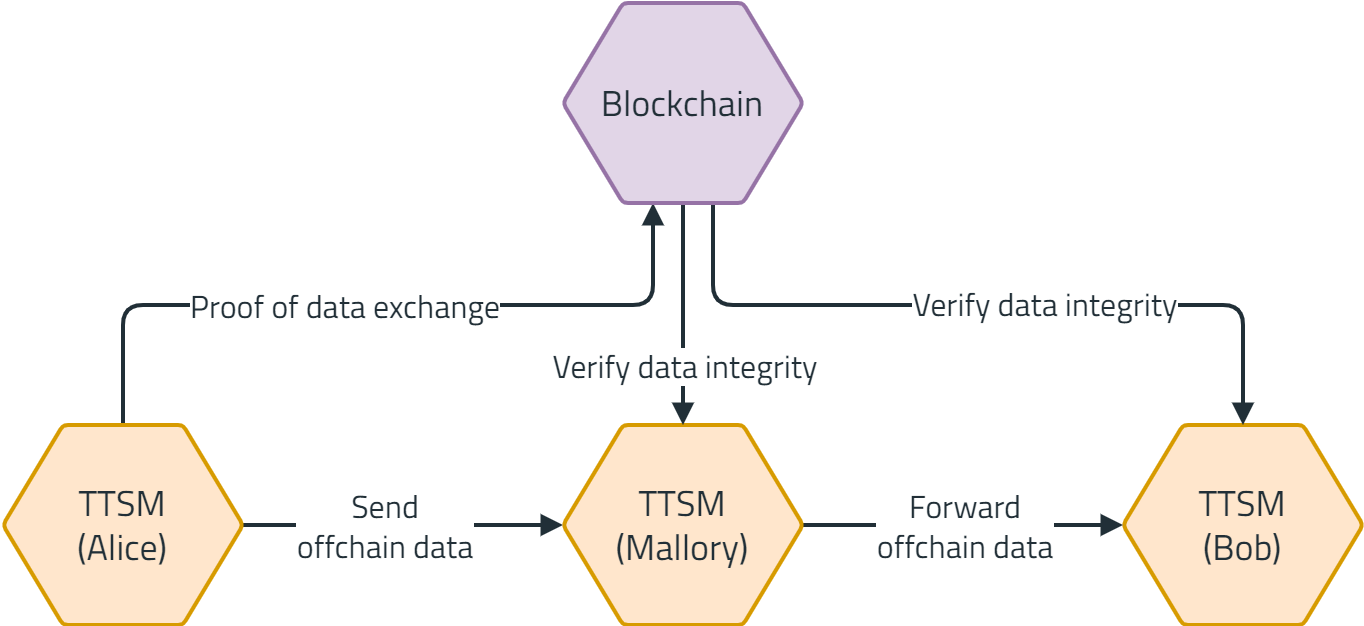
\includegraphics[width=.8\textwidth]{evaluation/graphics/static-analysis/TTSM-multiple-participants-broken-connection-2.drawio.png}}
    \caption{Mallory forwards messages from Alice to Bob.}
    \label{fig:evaluation:static_analysis:partially_connected_mesh}
\end{figure}

Setups like these are one possible mechanism supported by a \gls{ttsm} network that allows compensation of direct peer-to-peer links being lost. However, each participant must retain her connection to the blockchain to persist proof of data being exchanged and to verify the integrity of (forwarded) messages. Imagine a scenario where Alice dispatches a state transition request that Mallory must forward to Bob to complete the state transition. Instead of forwarding the original request dispatched by Alice, Mallory modifies it to make Bob accept the message and tamper with the state in a way that favors Mallory slightly and puts Bob at a disadvantage. Even though such attacks might be dangerous because they reduce the overall trust in the network, it is possible for Alice, and especially Bob, to verify the integrity of the forwarded message using the blockchain\footnote{For example, by comparing the hash of the forwarded message with the hash stored on the blockchain.}.

To better integrate compensation mechanisms into the \gls{ttsm} concept, a new consistency message that proves that a participant has indeed forwarded a message could be introduced. Two opportunities for future work have been identified:

\begin{itemize}
    \item The investigation of compensation mechanisms for lost peer-to-peer or even peer-to-blockchain connections to further increase resiliency.
    \item The investigation of algorithms with a small on-chain footprint that allow participants to verify message integrity.
\end{itemize}

Furthermore, this section has shown that the number of blockchain transactions required is linear to the number of participants involved in a particular state transition and that the number of persistence events dispatched internally by a \gls{ttsm} is strictly larger. Internal persistence events are not only dispatched for each blockchain transaction (associated with a commitment reference), but they can also be used for everything that happens only on the side of a single participant that is irrelevant for other participants. This enables a \gls{ttsm} to give participants a much finer granularity on traceability without polluting the blockchain.



\section{Scenario Simulations}
\label{sec:evaluation:simulations}
The aim of this section is to show the real-world utility of the approach proposed in this work. Different use cases are therefore simulated to conduct an experimental analysis of the concept and its prototypical implementation. Furthermore, with a strong focus on execution cost and latency, the results are compared with approaches from related work. The primary sources, used as baseline references for the upcoming evaluation, include the approaches proposed by Prybila et al.~\cite{runtime_verification_for_bp_utilizing_bitcoin}, who conducted a thorough evaluation of the execution duration of their approach, Weber et al.~\cite{untrusted_bp_execution_using_blockchain} who gave an overview of the execution cost and latency when applying their concept to a supply chain and incident management use case, and Loukil et al.~\cite{interpreted_bp_on_blockchain_loukil} who evaluated their approach against two compiled and two interpreted concepts from related literature regarding execution cost.


\subsection{Prototype Adaptations}
\label{sec:evaluation:simulations:adaptations}
Even though the high flexibility of the proposed concept, as shown in section~\ref{sec:evaluation:qualitative_analysis:flexibility_criteria}, would allow the usage of an arbitrary blockchain or layer-2 rollup, an \gls{evm}-based approach is used to improve comparability with existing approaches from related literature. Using the \gls{evm} furthermore allows Solidity byte code to be converted and ported to other blockchains and rollups such as zkSync\footnote{\url{https://zksync.io/} (accessed on 2022-11-25)} or Optimism\footnote{\url{https://optimism.io/} (accessed on 2022-11-25)} as well. The \gls{evm} consistency strategy implemented for this evaluation creates a fully connected peer-to-peer mesh network where each participant directly communicates with all the other participants. In addition, each participant establishes a connection to the \gls{evm} to store the SHA-256 hash of the exchanged message on-chain. The smart contract developed and deployed for this purpose is shown in code listing~\ref{lst:evaluation:simulations:hash_storage}.\\

\begin{lstlisting}[language=Solidity,caption=Implementation of a smart contract that stores message hashes,captionpos=b,label=lst:evaluation:simulations:hash_storage]
pragma solidity >=0.7.0 <0.9.0;

/**
 * @title Hash Storage
 * @dev Store 256-bit hash values as event log
 */
contract HashStorage {

    /**
     * @dev Stores all hashes in an event log. Using events reduces gas cost dramatically.
     */
    event StoreHash(bytes32 hash);

    /**
     * @dev Stores the given hash values as event log.
     */
    function store(bytes32 hash) public {
        emit StoreHash(hash);
    }
}
\end{lstlisting}

This very simplistic smart contract only allows the storage of 256-bit values, which is exactly the amount of data an SHA-256 hash requires. To further reduce cost, the hashes are stored as event logs only. This enables traceability but omits the need for expensive $G_{sset}$ operations with a gas cost of $20000$, only leaving a $G_{transaction}$ operation as the single most expensive operation with $21000$ gas in this smart contact. With $G_{log}$ and $G_{logtopic}$ requiring $375$ gas, and $G_{logdata}$ only requiring $8$ gas per byte stored, each hash persisted on the \gls{evm} requires less than $23000$ gas~\cite{ethereum_yellow_paper}. The integrity of an exchanged message can then be verified by fetching the transaction receipt and testing if the hash stored on the \gls{evm} is the same as the hash of the message's payload. This process is part of the \gls{evm} strategy and is depicted in code listing~\ref{lst:evaluation:simulations:verifying_received_messages}.\\ % chktex 35

\begin{lstlisting}[language=JavaScript,caption=Implementation of the verification process of messages received,captionpos=b,label=lst:evaluation:simulations:verifying_received_messages]
async receiveConsistencyMessage<T>(msg: ConsistencyMessage<T>) {

  // Retrieve transaction receipt to check if log contains correct message hash.
  const txHash = msg.commitmentReference.transactionHash;
  const tx = await Web3.eth.getTransactionReceipt(txHash);

  // Reject the message if the expected and the actual hash of the message payload differ.
  const expectedHash = tx.logs[0].data;
  const actualHash = sha256(JSON.stringify(msg.payload));
  if (expectedHash !== actualHash) {
    return 'INVALID_HASH';
  }

  // Pass the message on to other modules.
  actions$.next(msg);
  return 'OK';
}
\end{lstlisting}

If the hash differs from what has been stored on the \gls{evm}, the message is entirely omitted because its integrity cannot be verified. For reproducibility reasons, the simulations rely entirely on the \gls{evm} strategy described above. The prototypical implementation used for this evaluation is available GitHub\footnote{\url{https://github.com/danielkleebinder/ttsm-prototype} (accessed on 2022-11-29)}. The upcoming sections introduce the use cases the prototype is evaluated against, derive corresponding \gls{bpmn} diagrams, and afterwards discuss the results of the simulation runs and compare them to results from related literature.


\subsection{Scenario Descriptions}
\label{sec:evaluation:simulations:descriptions}
Three distinct scenarios have been chosen for the evaluation of the proposed concept. The first one simulates a simplified facility maintenance use case that has been created throughout the course of this work by conducting interviews with domain experts - introduced in section~\ref{sec:background:bpm:bpmn}, this scenario aims to show real-world utility of the proposed concept. The second scenario simulates a supply chain, and the third a software incident management use case as described and adapted by Weber et al.~\cite{untrusted_bp_execution_using_blockchain}, López-Pintado et al.~\cite{interpreted_bp_on_blockchain_weber}, and Loukil et al.~\cite{interpreted_bp_on_blockchain_loukil} to improve comparability and reproducibility of the results. The second and third scenarios are only briefly outlined and not further discussed.

\subsubsection{Facility Management}
\label{sec:evaluation:simulations:descriptions:fm}
The facility maintenance use case, as already partially introduced in section~\ref{sec:background:bpm:bpmn}, has been derived from interviews conducted with real-world domain experts. It describes a scenario where a building administrator has been notified\footnote{Either through a timely trigger or thorough inspection conducted by a third party, for example.} that maintenance on a facility inside the building\footnote{This might be an elevator, a vending machine, or an escalator, for example} is due. The building administrator now contacts an external maintenance contractor and prepares the facility for further inspections and the maintenance itself\footnote{By closing off the facility site, for example.}. Afterwards, the contractor starts performing the maintenance, orders spare parts if repairs are required, and sends the building administrator a notice that maintenance has been completed. After the administrator's successful inspection of the facility, the maintenance contractor sends an invoice and a maintenance report. The \gls{bpmn} diagram of this scenario is depicted in figure~\ref{fig:evaluation:simulations:maintenance_full}.

\begin{figure}[h]
    \makebox[\textwidth][c]{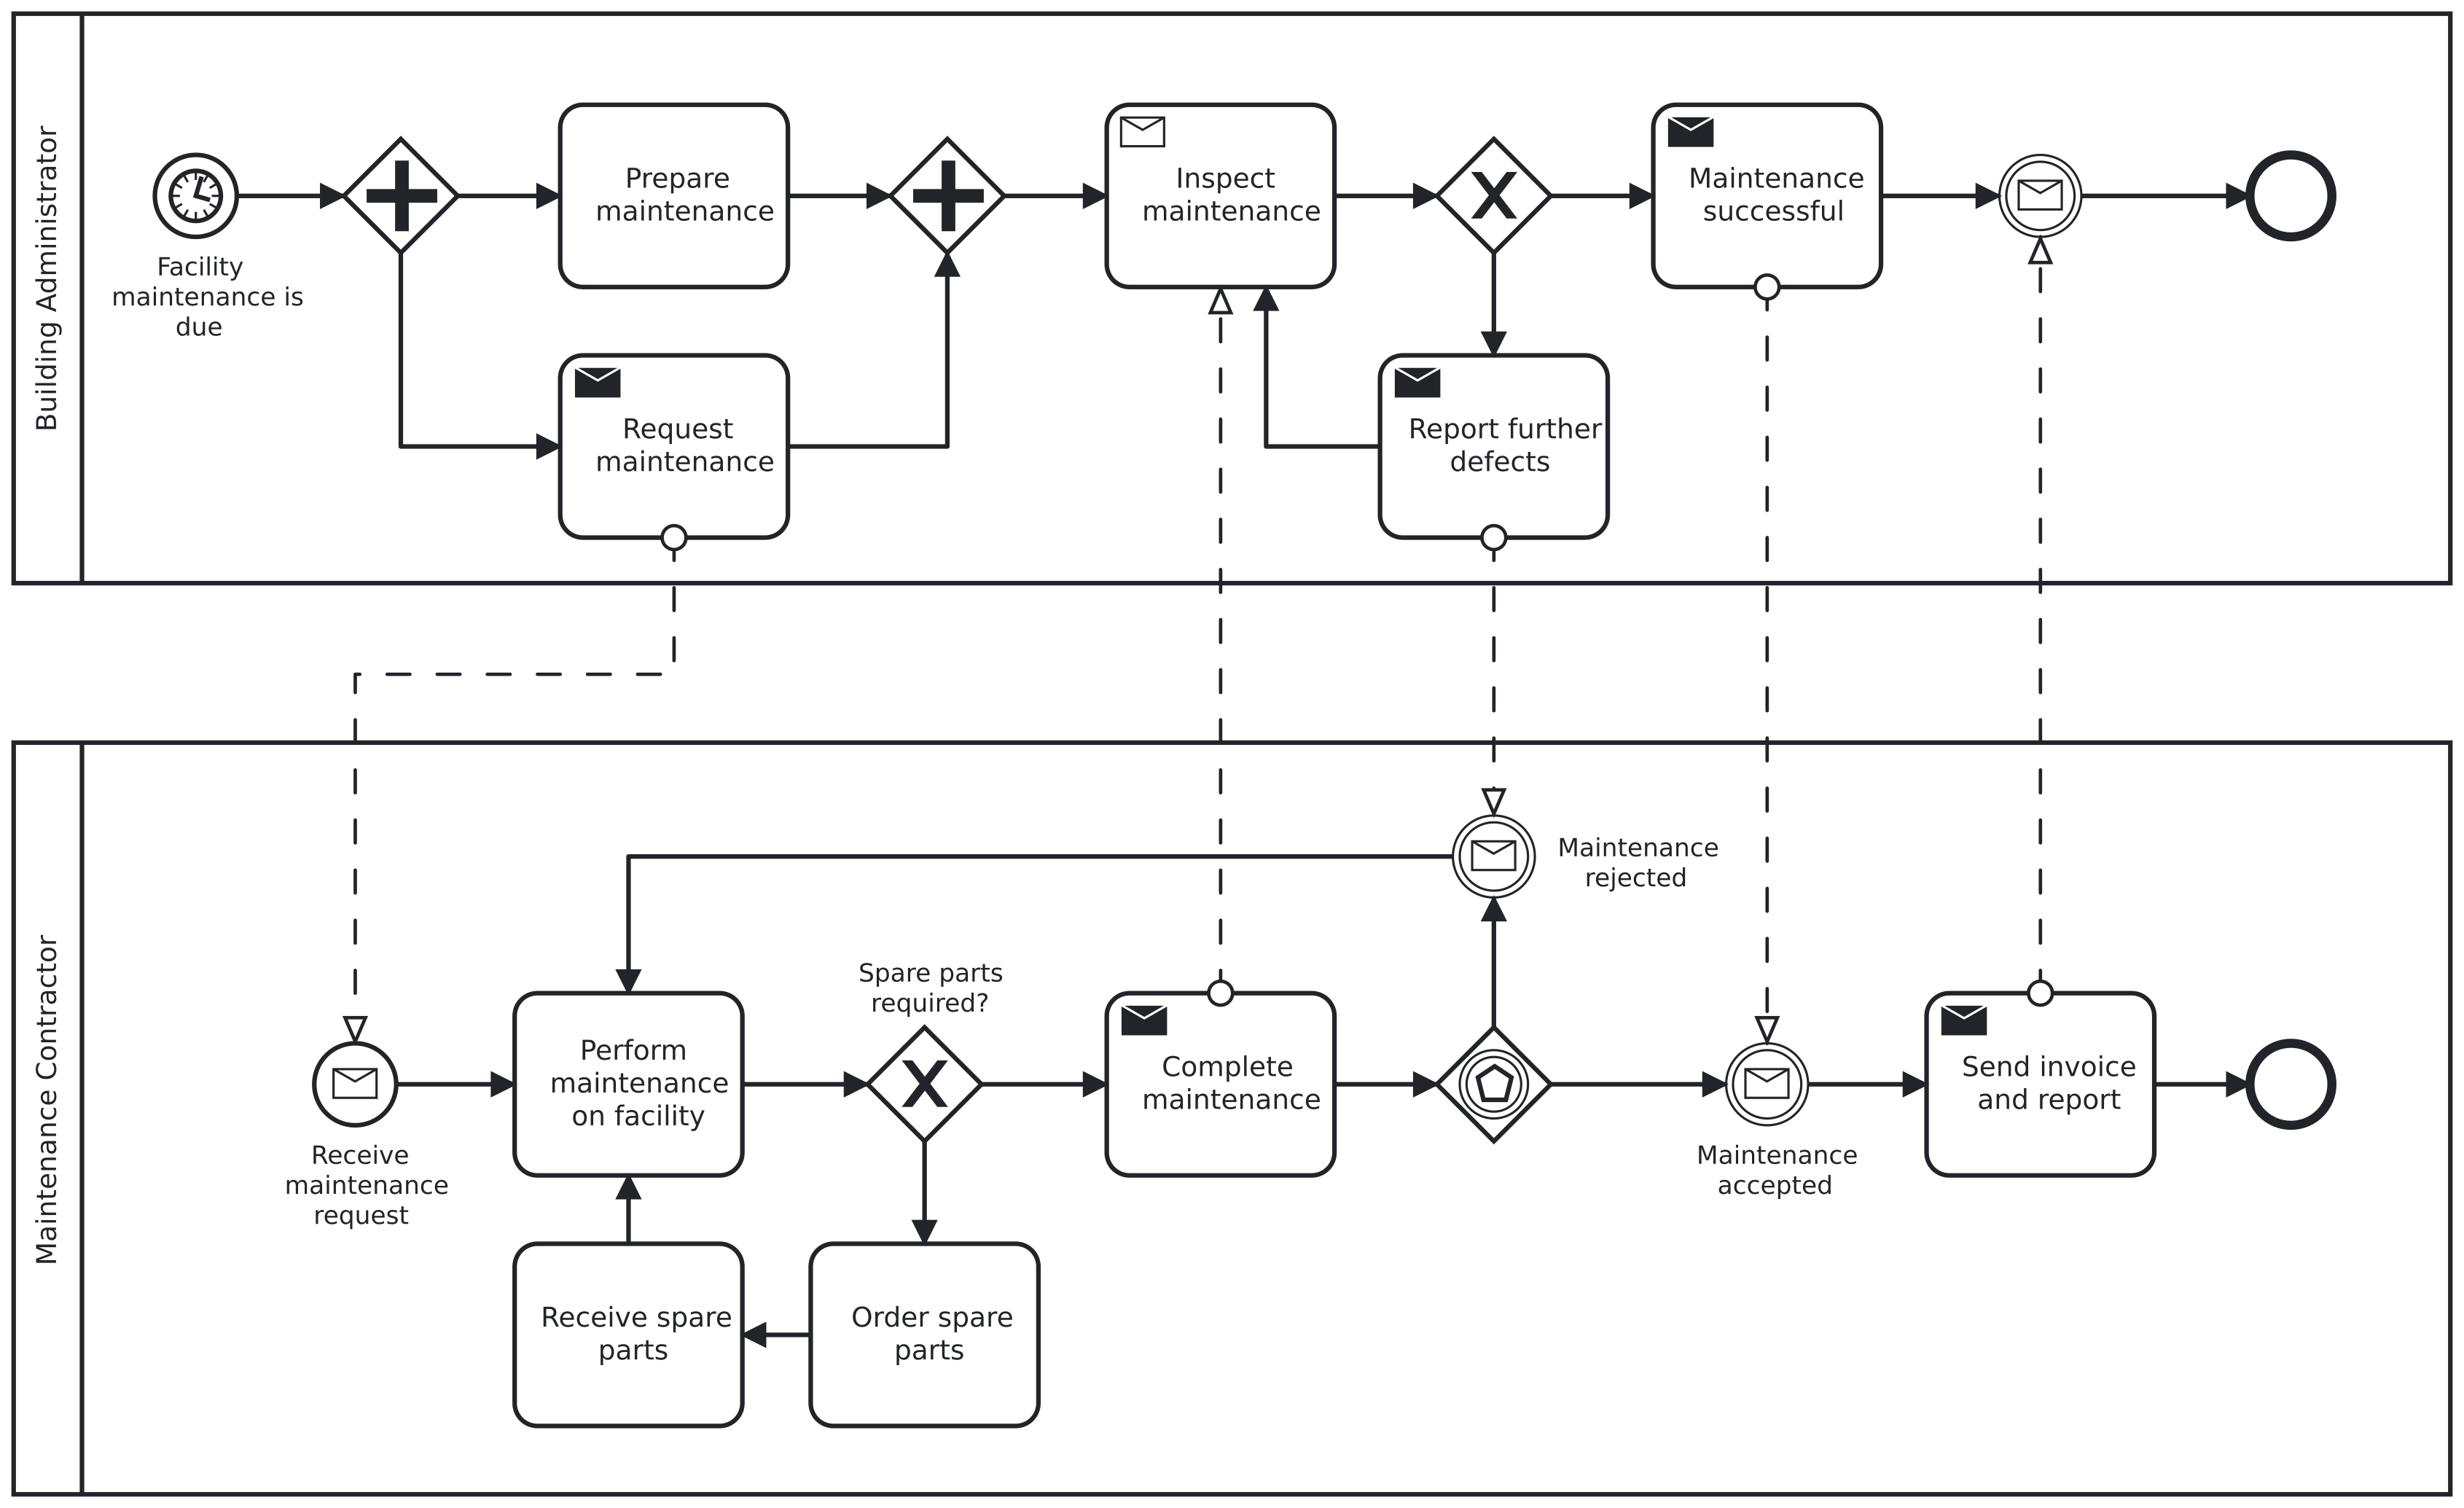
\includegraphics[width=\textwidth]{background/graphics/maintenance-full.png}}
    \caption{BPMN diagram of the facility maintenance use case introduced in~\ref{sec:background:bpm:bpmn}.}
    \label{fig:evaluation:simulations:maintenance_full}
\end{figure}

This use case should demonstrate the real-world utility of the proposed \gls{ttsm} approach. It has been simplified to some extent to use it as a stepping stone towards more complex scenarios. However, it illustrates the use of parallel and exclusive gates and the exchange of messages between participants. Therefore, the facility management scenario is an excellent first scenario to show that the proposed concept would indeed be functional in real-world environments.

\subsubsection{Supply Chain}
\label{sec:evaluation:simulations:descriptions:sc}
The supply chain use case is commonly used in related work to demonstrate the utility of a new approach and to compare its cost with other approaches. First introduced by Fdhila et al.~\cite{fdhila2015_change_in_collaborative_bps}, Weber et al.\ adapted and simplified this scenario in their work~\cite{untrusted_bp_execution_using_blockchain}. It consists of five participants interacting with each other. A bulk buyer orders a product from a manufacturer. The manufacturer then calculates what supplies in the form of raw materials and basic resources are required to produce this product and orders them from a middleman. The middleman forwards the order for the required supplies, and a carrier transports them from the supplier to the manufacturer. The manufacturer then produces the requested product and delivers it to the bulk buyer.

\begin{figure}[h]
    \makebox[\textwidth][c]{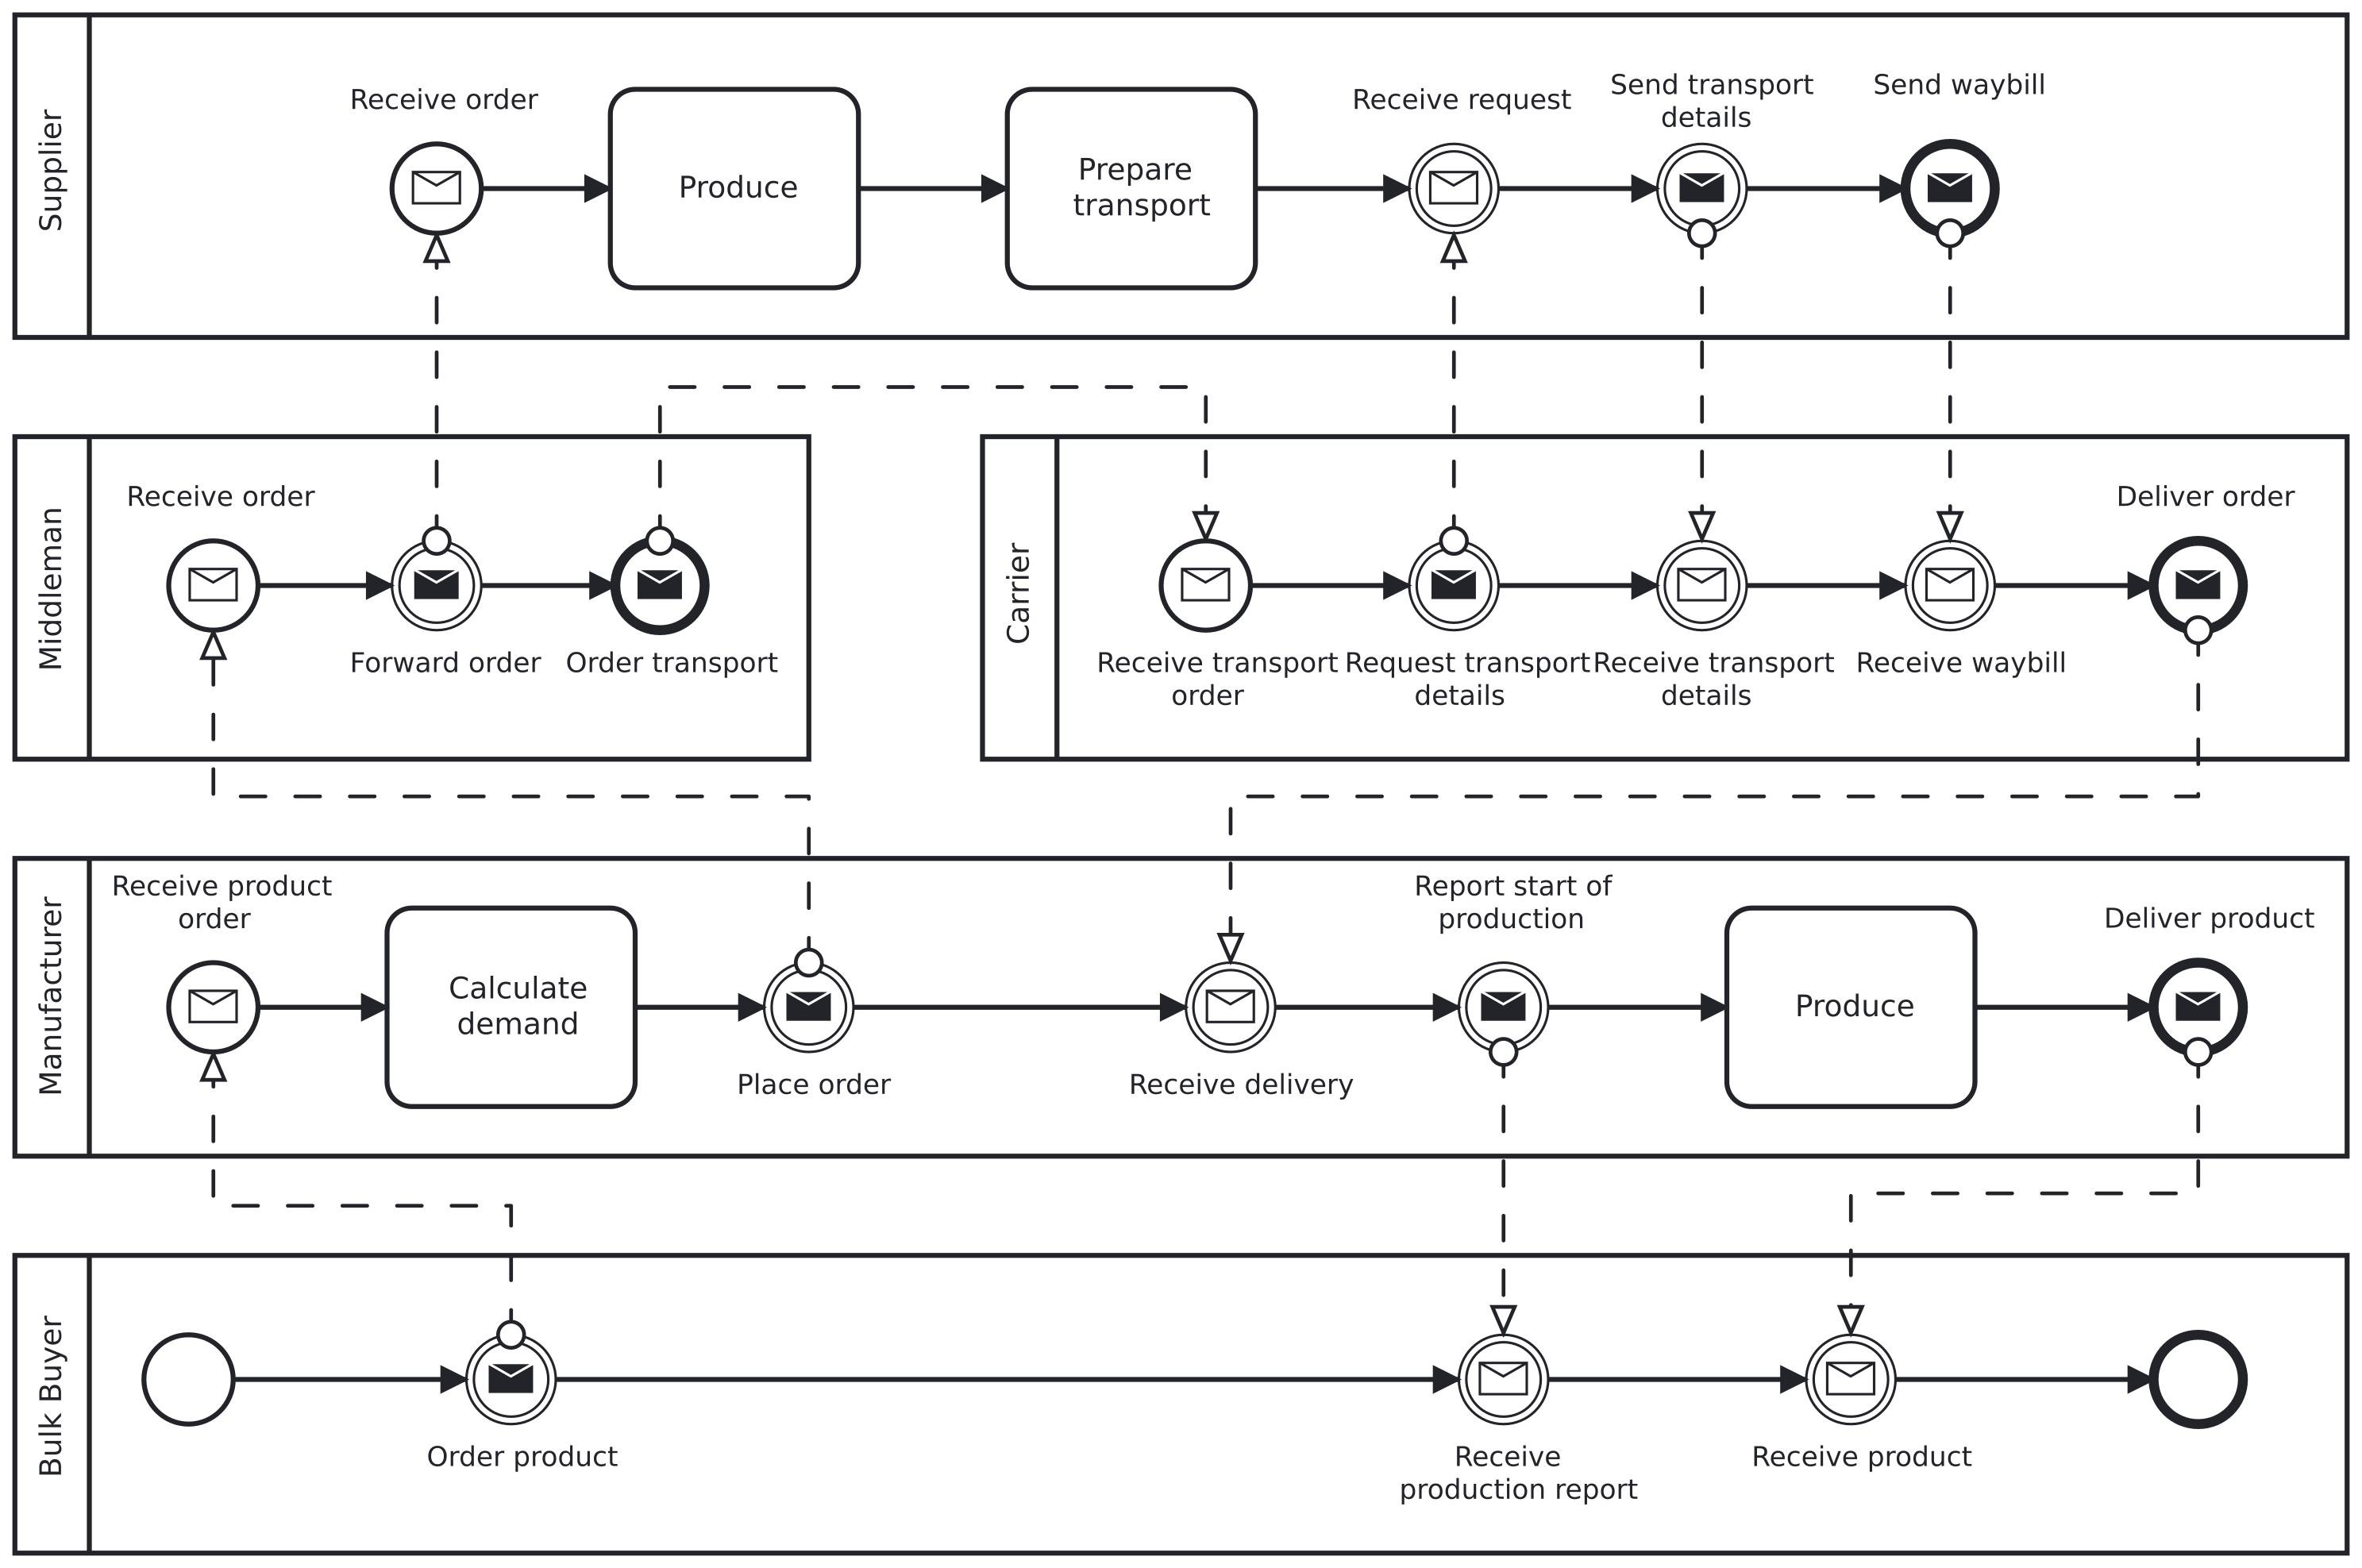
\includegraphics[width=\textwidth]{evaluation/graphics/experimental-analysis/supply-chain.png}}
    \caption{BPMN diagram of a supply chain adapted from Weber et al.~\cite{untrusted_bp_execution_using_blockchain}.}
    \label{fig:evaluation:simulations:supply_chain_full}
\end{figure}

One might realize that this supply chain has much conflict potential. Imagine the bulk buyer ordering a product that must arrive before a deadline. If the deadline is not met by the manufacturer, she has to pay penalties. To be on time, the manufacturer orders supplies through the middleman. However, the requested supplies arrived three days later than expected and were not in the correct quantity. This puts the manufacturer, whose time frame now has shifted, in a tough spot and the carrier since the manufacturer might refuse to accept the incomplete delivery. Therefore, the supply chain scenario can be used quite well to demonstrate conflict resolution capabilities~\cite{untrusted_bp_execution_using_blockchain,interpreted_bp_on_blockchain_loukil}.

\subsubsection{Incident Management}
\label{sec:evaluation:simulations:descriptions:im}
The incident management use case is, similar to the supply chain use case, a commonly encountered scenario in related work. First discussed in ``BPMN 2.0 by Example''~\cite{omg2010_bpmn_by_example}, it found its way into the domain of workflow execution on the blockchain through Weber et al.~\cite{untrusted_bp_execution_using_blockchain} and was then further adapted by many more authors in the sense of design science for comparability reasons~\cite{optimized_execution_of_bp_using_petri_nets_on_blockchain,interpreted_bp_on_blockchain_weber,lean_architecture_for_blockchain_based_process_execution,interpreted_bp_on_blockchain_loukil}.

\begin{figure}[h]
    \makebox[\textwidth][c]{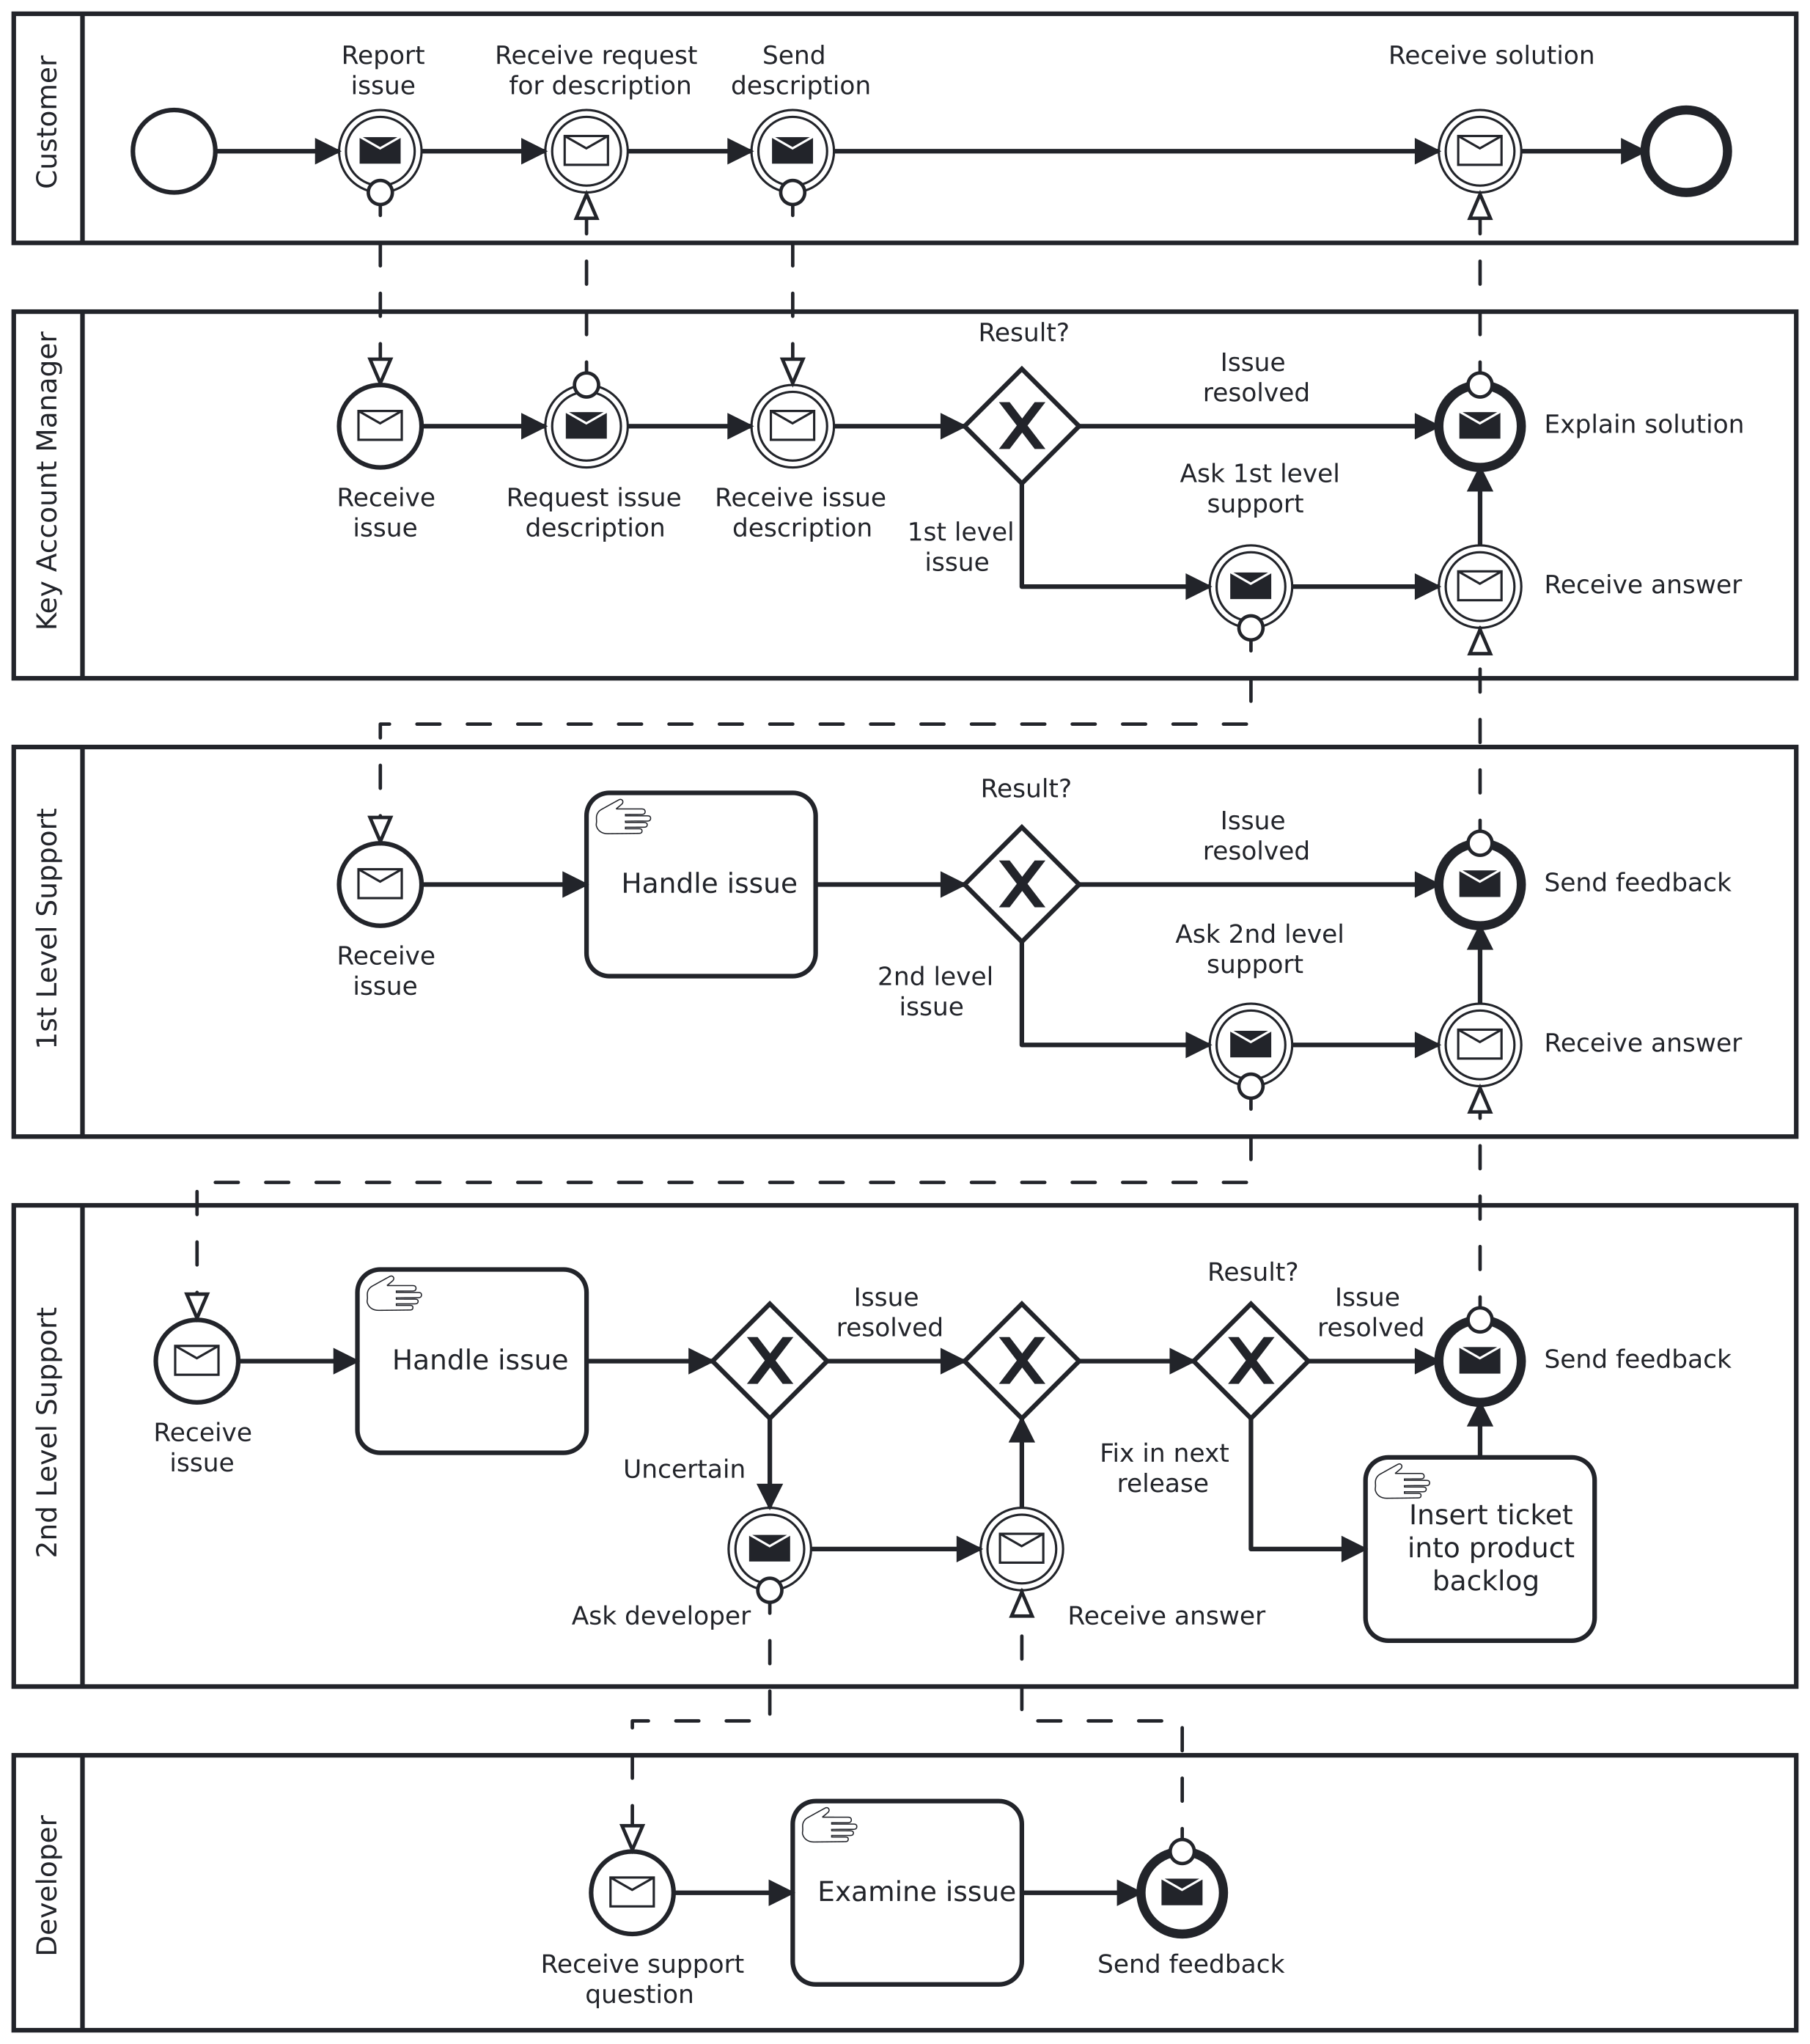
\includegraphics[width=.8\textwidth]{evaluation/graphics/experimental-analysis/incident-management.png}}
    \caption{BPMN diagram of the incident management use case adapted from ``BPMN 2.0 by Example''~\cite{omg2010_bpmn_by_example}.}
    \label{fig:evaluation:simulations:incident_management_full}
\end{figure}

Figure~\ref{fig:evaluation:simulations:incident_management_full} depicts the \gls{bpmn} diagram of the entire incident management use case. It follows an issue reported by a customer who noticed a problem with a particular software component. The issue then goes through multiple support layers, starting with the key account manager. If the key account manager cannot solve the issue by herself, she hands it over to the 1\textsuperscript{st} level support. If the 1\textsuperscript{st} level support cannot resolve the issue, it is passed on to the 2\textsuperscript{nd} level support who either asks a software developer for assistance or immediately creates a ticket and puts it into the products backlog. This relatively sophisticated business process includes more gateways and a strict separation of participants\footnote{Developers can only talk to 2\textsuperscript{nd} level support, 2\textsuperscript{nd} level support can only talk to developers and 1\textsuperscript{st} level support and so on.}.


\subsection{Discussion of Results}
\label{sec:evaluation:simulations:summary}
The evaluation results in the upcoming sections have been obtained by extracting only the communication between participants as choreography diagrams. The choreography diagram for the facility management scenario is depicted in figure~\ref{fig:background:maintenance_full_choreography}. For the supply chain and incident management scenarios, the same choreography diagrams have been used as in the related literature. These diagrams are both depicted in the work of Loukil et al.~\cite{interpreted_bp_on_blockchain_loukil}. Afterwards, semantically equivalent statecharts have been derived using the Stately editor\footnote{\url{https://stately.ai/} (accessed on 2022-10-10)} and fed into the \gls{ttsm} prototype. Finally, a script was employed to automate the process of deploying, instantiating, and executing the scenarios to ensure that each sample is executed with comparable constraints and conditions. Table~\ref{tab:evaluation:simulations:structural_comparison} gives a brief overview of the structure of each scenario.

\begin{table}[h]
\centering
\begin{tabular}{|l|r|r|r|}
    \hline
    \textbf{Scenario} & \textbf{Participants} & \textbf{Tasks} & \textbf{Gateways} \\
    \hline
    Facility Maintenance & 2 & 5 & 1 \\
    Supply Chain & 5 & 10 & 2 \\
    Incident Management & 5 & 9 & 6 \\
    \hline
\end{tabular}
\caption{Structural comparison of the choreography diagrams and statecharts of the evaluated scenarios}
\label{tab:evaluation:simulations:structural_comparison}
\end{table}

The supply chain and incident management scenarios used in this work have the same structural properties as those used for evaluation in related literature~\cite{untrusted_bp_execution_using_blockchain,optimized_execution_of_bp_using_petri_nets_on_blockchain,interpreted_bp_on_blockchain_weber,lean_architecture_for_blockchain_based_process_execution,interpreted_bp_on_blockchain_loukil}. This not only improves comparability but also reproducibility of the results. The evaluation itself is also fully automated and can be triggered after setting up the prototype project and specifying an applicable consistency strategy.

\subsubsection{Confirmation Correctness}
\label{sec:evaluation:simulations:confirmation_correctness}
The capabilities of detecting incorrect workflow traces have been evaluated according to the methodologies defined by Weber et al.~\cite{untrusted_bp_execution_using_blockchain} and Loukil et al.~\cite{interpreted_bp_on_blockchain_loukil}. A workflow trace is a path from one task in a workflow instance to another final task. For the evaluation, 500 traces have been randomly generated by shuffling a predefined set of all state transitions $T$ of a given workflow $W$ to generate a new set of distinct traces $D$, where $D$ has a cardinality of 500. Furthermore, $\forall T' \in D: T' = T$, however, $T'$ has a unique permutation of elements in $D$. This results in two subsets $D_{c} \subseteq D$ and $D_{n} \subseteq D$, where $D_{c}$ is the set of conforming traces\footnote{Traces that can be used in a given workflow.} and $D_{n}$ the set of non-conforming traces\footnote{Traces that cannot be used in a given workflow.} such that $D_{c} \cap D_{n} = \emptyset$. All traces have been correctly identified by the \gls{ttsm} prototype according to their correctness. A list of the results per scenario can be found in table~\ref{tab:evaluation:simulations:confirmation_correctness}.

\begin{table}[h]
\centering
\begin{tabular}{|l|r|c|c|}
    \hline
    \textbf{Scenario} & \textbf{Type} & \textbf{Samples} & \textbf{Correctness} \\
    \hline
    Facility Maintenance & Conforming     & 206 & 100\% \\
                         & Non-Conforming & 294 & 100\% \\
    Supply Chain         & Conforming     & 180 & 100\% \\
                         & Non-Conforming & 320 & 100\% \\
    Incident Management  & Conforming     & 197 & 100\% \\
                         & Non-Conforming & 303 & 100\% \\
    \hline
\end{tabular}
\caption{Average execution duration of each scenario}
\label{tab:evaluation:simulations:confirmation_correctness}
\end{table}

The results show that the proposed concept performs equally as well as existing solutions regarding the identification of correct and incorrect traces~\cite{untrusted_bp_execution_using_blockchain,interpreted_bp_on_blockchain_loukil}. Nonetheless, the \gls{ttsm} prototype has shown better resiliency and a higher tolerance for conforming traces because it can recover when an invalid state transition event has been dispatched. This is caused by the underlying XState library that ignores invalid state transitions and preserves the current state. Overall, the results presented in this section are in line with expectations.

\subsubsection{Blockchain imposed Latency}
\label{sec:evaluation:simulations:execution_duration}
Overall latency of the system and ensuring finality or even just inclusion of commands into blocks by a \gls{ttsm} are expected to be tightly coupled to the block time of the chosen \gls{bct}. Methodologies from related work such as Prybila et al.~\cite{runtime_verification_for_bp_utilizing_bitcoin}, and Weber et al.~\cite{untrusted_bp_execution_using_blockchain} have been employed to further investigate latency imposed by the transaction inclusion duration\footnote{Also referred to as consistency and persistence properties of a \gls{ttsm} (see section~\ref{sec:ttsm:properties}).} of the system. For the evaluation, it is assumed that all participants are available at any time.

As of section~\ref{sec:ttsm:proposal}, commands in a \gls{ttsm} are dispatched into the network of workflow participants and accepted or rejected by each of them. This is a two-step process which, if transactions are required to be included into a block of a blockchain before the \gls{ttsm} can continue, requires at least two blocks to be produced --- one in which the command is proposed and one in which participants accepted or rejected the command. The average transaction inclusion time is determined by the central limit theorem given in equation~\ref{eq:evaluation:simulations:central_limit_theorem} where $\mu$ is the overall mean of the random samples $X_1,X_2,\ldots,X_n,\ldots$, while $\bar{X}_{n}$ is the mean of the first $n$ samples and $\sigma_{\bar{X}}=\sigma/\sqrt{n}$ with $\sigma^2$ being the variance.

\begin{equation}
\label{eq:evaluation:simulations:central_limit_theorem}
Z=\lim_{n \to \infty}\left(\frac{\bar{X}_{n} - \mu}{\sigma_{\bar{X}}}\right)
\end{equation}

Given that completely finalizing a command takes at least two blocks, the median of the normal distribution is $\frac{3}{2} \cdot b_t$ where $b_t$ is the average block time. This assumption is supported by the empirical evaluation results in table~\ref{tab:evaluation:simulations:transaction_inclusion_duration} equally for all types of commands across all scenarios. Regarding the simulation itself, at the time of writing this work, there are two proof-of-stake test networks available for Ethereum in particular, namely Sepolia\footnote{\url{https://sepolia.dev/} (accessed on 2022-11-25)} and Goerli\footnote{\url{https://goerli.net/} (accessed on 2022-11-25)}. In conjunction with Alchemy\footnote{\url{https://alchemy.com/} (accessed on 2022-11-25)}, a platform that provides tooling for web3 development, Goerli was used to run the simulations. All simulations used the same smart contract which was previously deployed --- this is similar to how a \gls{ttsm} would operate on the Ethereum main network in real-world scenarios as well. Afterwards, the workflow for each use case (facility management, supply chain and incident management) were created and instantiated exactly 50 times. After successful instantiation, each workflow was executed 10 times which results in the depicted number of samples in table~\ref{tab:evaluation:simulations:transaction_inclusion_duration} below.

\begin{table}[h]
\centering
\begin{tabular}{|l|c|c|c|}
    \hline
    & \multicolumn{3}{c|}{\bfseries Facility Management} \\ \cline{2-4}
    & Samples & Av.\ Duration & Std. Dev. ($\sigma$) \\
    \hline
    Workflow Definition    & 50  & 18.209 s & 3.8 s \\
    Workflow Instantiation & 50  & 17.847 s & 3.6 s \\
    State Transition       & 50  & 17.921 s & 3.1 s \\
    \hline
    & \multicolumn{3}{c|}{\bfseries Supply Chain} \\ \cline{2-4}
    & Samples & Av.\ Duration & Std. Dev. ($\sigma$) \\
    \hline
    Workflow Definition    & 50  & 17.383 s & 3.5 s \\
    Workflow Instantiation & 50  & 18.619 s & 3.9 s \\
    State Transition       & 100 & 17.441 s & 3.5 s \\
    \hline
    & \multicolumn{3}{c|}{\bfseries Incident Management} \\ \cline{2-4}
    & Samples & Av.\ Duration & Std. Dev. ($\sigma$) \\
    \hline
    Workflow Definition    & 50  & 17.538 s & 3.4 s \\
    Workflow Instantiation & 50  & 17.112 s & 3.7 s \\
    State Transition       & 90  & 17.985 s & 3.3 s \\
    \hline
\end{tabular}
\caption{Average duration of each operation type}
\label{tab:evaluation:simulations:transaction_inclusion_duration}
\end{table}

The results were extracted from multiple test runs of the \gls{ttsm} prototype. Given that the block time of Ethereum, and in this case the Goerli test network, averages at around 12 seconds, it takes at least $\frac{3}{2} \cdot 12 = 18$ seconds to ensure that a command, including the participants responses, has been integrated into a new block on the blockchain. However, the standard deviation $\sigma$ of the samples is rather large. This distribution originates from the randomization of execution times for each command resulting in a 12 to 24 seconds execution duration. Some commands have been dispatched immediately after a new block has been mined, resulting in an overall duration of around two block times (i.e.,\ $24$ seconds), while others have been dispatched at the end of a block and thus have been integrated into said block almost immediately after dispatching, resulting in a duration of just above one block time (i.e.,\ $>12$ seconds). The execution duration distribution is depicted as box plot in figure~\ref{fig:evaluation:simulations:box_chart_transaction_inclusion}.

\begin{figure}[h]
    \makebox[\textwidth][c]{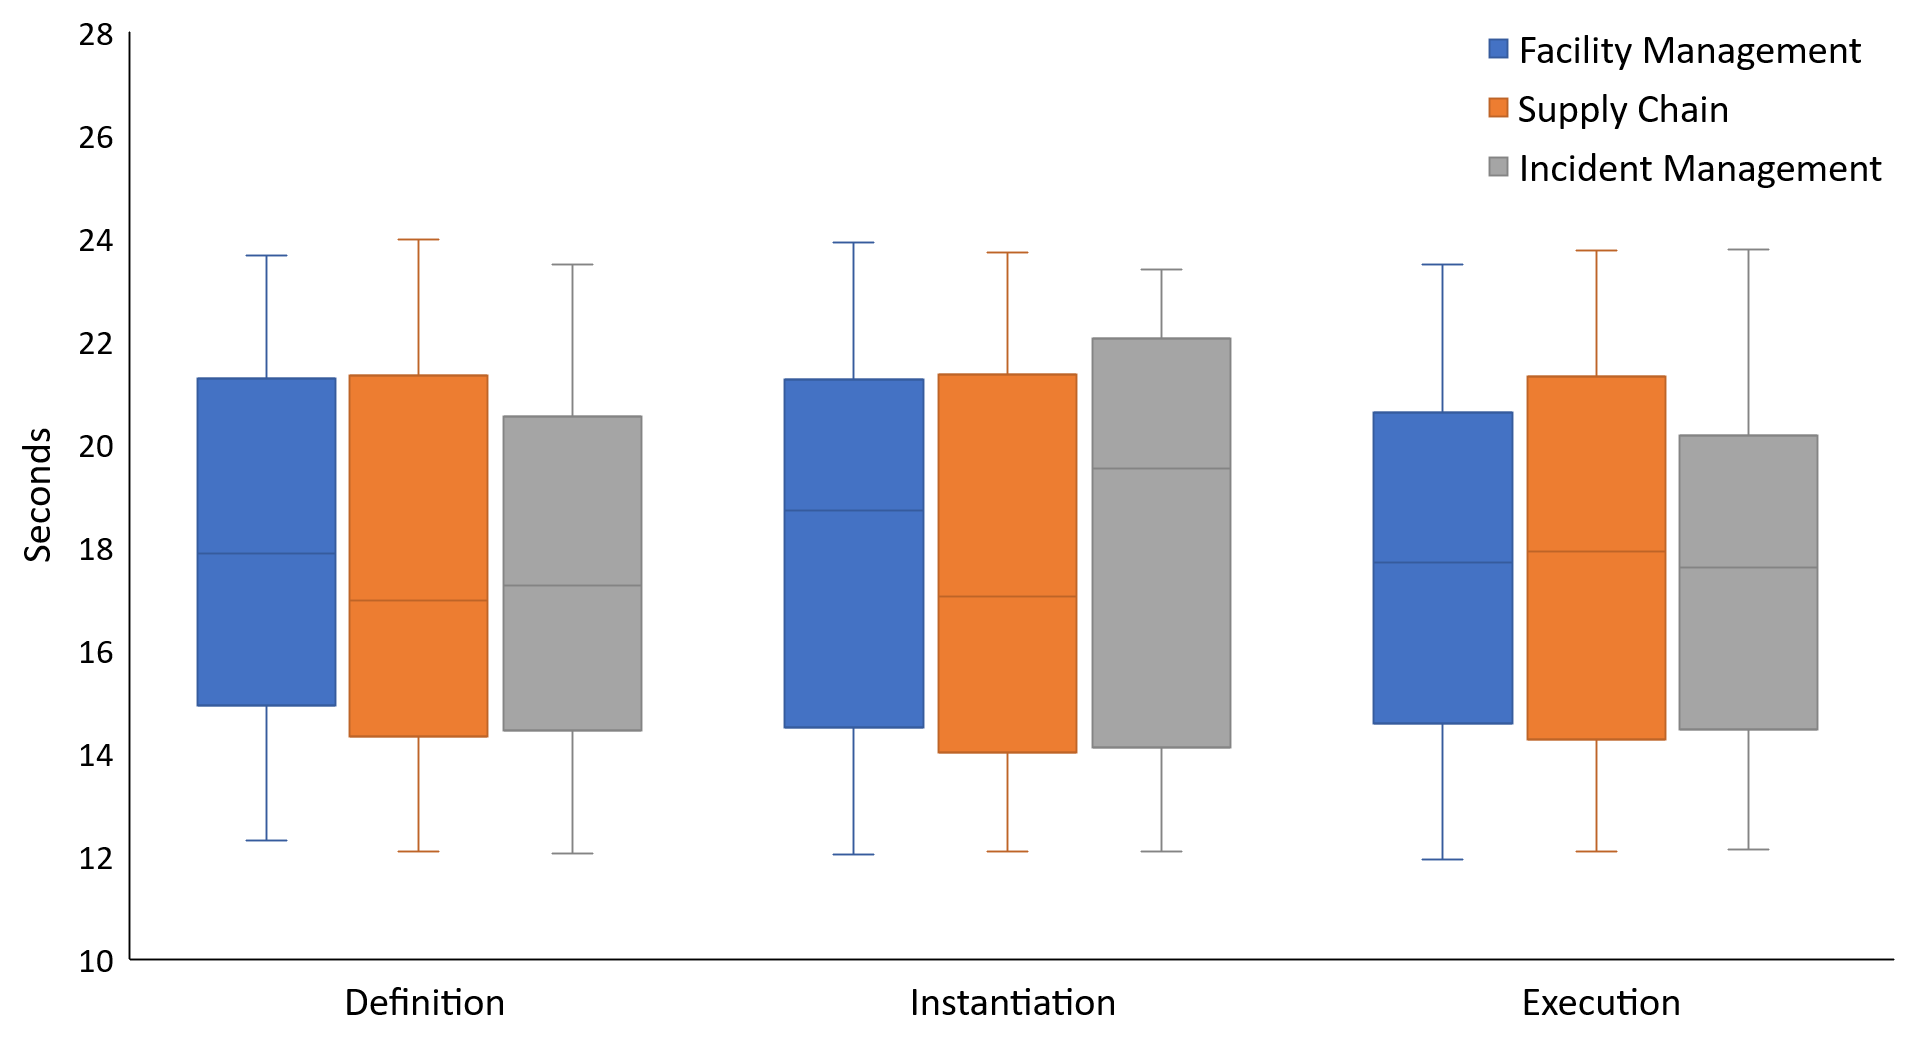
\includegraphics[width=.85\textwidth]{evaluation/graphics/experimental-analysis/enforced-finality-box-chart.png}}
    \caption{Box plot illustrating a one to two block time (12 s -- 24 s) command duration imposed by the blockchain.}
    \label{fig:evaluation:simulations:box_chart_transaction_inclusion}
\end{figure}

Nonetheless, the proposed \gls{ttsm} concept technically also supports \textit{optimistic workflow execution}. This kind of execution aims to eliminate the latency introduced by the blockchain. It enables participants to dispatch and distribute new commands to the workflow network without having to wait until the blockchain has produced a new block in which an integrity proof of the command is included. The aim of optimistic workflow execution\footnote{Later on also referred to as \textit{optimistic execution}.} is to create a system that is close to the status quo of off-chain \gls{bpm} engines regarding workflow execution duration and performance. While \textit{enforced transaction inclusion}\footnote{Later on also referred to as \textit{enforced inclusion}.} halts workflow execution while waiting for the command integrity transaction to be included in the next block\footnote{Which is required to generate a blockchain transaction receipt holding the commitment reference.}, \textit{optimistic execution} immediately sends the command to all involved participants and afterwards waits for the blockchain response.

If the participant who dispatched the optimistic command eventually receives the transaction receipt, she creates a new consistency event that associates the optimistic command with the commitment reference from the receipt. Even though \textit{optimistic execution} is much faster than \textit{enforced inclusion}, participants must expect rollbacks at a later point in time when the blockchain catches up. If the integrity transaction cannot be included in a block on the blockchain or if any of the participants notice that an outstanding optimistic command is still missing its commitment reference after a predefined period of time, the command becomes invalid. This rolls the entire workflow state back to the point in time where it was still valid. The consistency and persistence events stored are still preserved inside the event bus for traceability reasons; however, the event sourcing systems of each particular module, which require a correct and consistent state, only accumulate events until the invalid one is reached. All events received after the rollback are then, once again, treated as valid ones.

Only a superficial \textit{optimistic execution} implementation is provided in the \gls{ttsm} prototype that eliminates the latency introduced by the blockchain but does not incorporate a rollback mechanism due to its complexity. Nonetheless, all scenarios have also been executed in this superficial \textit{optimistic execution} mode. The evaluation results are given in table~\ref{tab:evaluation:simulations:optimistic_duration}.

\begin{table}[h]
\centering
\begin{tabular}{|l|c|c|c|}
    \hline
    & \multicolumn{3}{c|}{\bfseries Facility Management} \\ \cline{2-4}
    & Samples & Av.\ Duration & Std. Dev. ($\sigma$) \\
    \hline
    Workflow Definition    & 50  & 0.019 s & 0.008 s \\
    Workflow Instantiation & 50  & 0.331 s & 0.033 s \\
    State Transition       & 50  & 0.114 s & 0.055 s \\
    \hline
    & \multicolumn{3}{c|}{\bfseries Supply Chain} \\ \cline{2-4}
    & Samples & Av.\ Duration & Std. Dev. ($\sigma$) \\
    \hline
    Workflow Definition    & 50  & 0.018 s & 0.005 s \\
    Workflow Instantiation & 50  & 0.041 s & 0.019 s \\
    State Transition       & 100 & 0.079 s & 0.033 s \\
    \hline
    & \multicolumn{3}{c|}{\bfseries Incident Management} \\ \cline{2-4}
    & Samples & Av.\ Duration & Std. Dev. ($\sigma$) \\
    \hline
    Workflow Definition    & 50  & 0.019 s & 0.005 s \\
    Workflow Instantiation & 50  & 0.023 s & 0.006 s \\
    State Transition       & 90  & 0.184 s & 0.069 s \\
    \hline
\end{tabular}
\caption{Average duration of each operation type using \textit{optimistic execution}}
\label{tab:evaluation:simulations:optimistic_duration}
\end{table}

The execution duration per command has been reduced to the workflow logic and network latency itself, entirely omitting the delay imposed by the blockchain. Table~\ref{tab:evaluation:simulations:finality_vs_optimistic_total} compares the total workflow execution duration of each scenario using \textit{enforced transaction inclusion} and \textit{optimistic workflow execution} modes.

\begin{table}[h]
\centering
\begin{tabular}{|l|c|c|c|c|c|c|}
    \hline
    \multirow{2}{*}{\bfseries Scenario} &
    \multicolumn{3}{c|}{\bfseries Enforced Inclusion} &
    \multicolumn{3}{c|}{\bfseries Optimistic Execution} \\ \cline{2-7}
    & Samples & Av.\ Dur. & $\sigma$ & Samples & Av.\ Dur. & $\sigma$ \\
    \hline
    Facility Management & 10 & 57 s & 3.1 s & 10 & 0.57 s & 0.3 s  \\
    Supply Chain        & 10 & 181 s & 16.8 s & 10 & 0.79 s & 0.3 s \\
    Incident Management & 10 & 149 s & 10.3 s & 10 & 1.65 s & 0.5 s \\
    \hline
\end{tabular}
\caption{Total duration of finality enforced and optimistic workflow execution}
\label{tab:evaluation:simulations:finality_vs_optimistic_total}
\end{table}

As illustrated before, choosing one execution mode over the other has a significant impact on the overall duration. When using \textit{enforced inclusion} mode, waiting for the command integrity transaction to be included in a new block on the Ethereum blockchain imposes a noteworthy latency. Figure~\ref{fig:evaluation:simulations:pie_chart_transaction_inclusion_portion} shows a pie chart depicting the duration required for the execution of the workflow logic (including network delays) and puts it against the downtime that transaction inclusion requires when explicitly enforced.

\begin{figure}[h]
    \makebox[\textwidth][c]{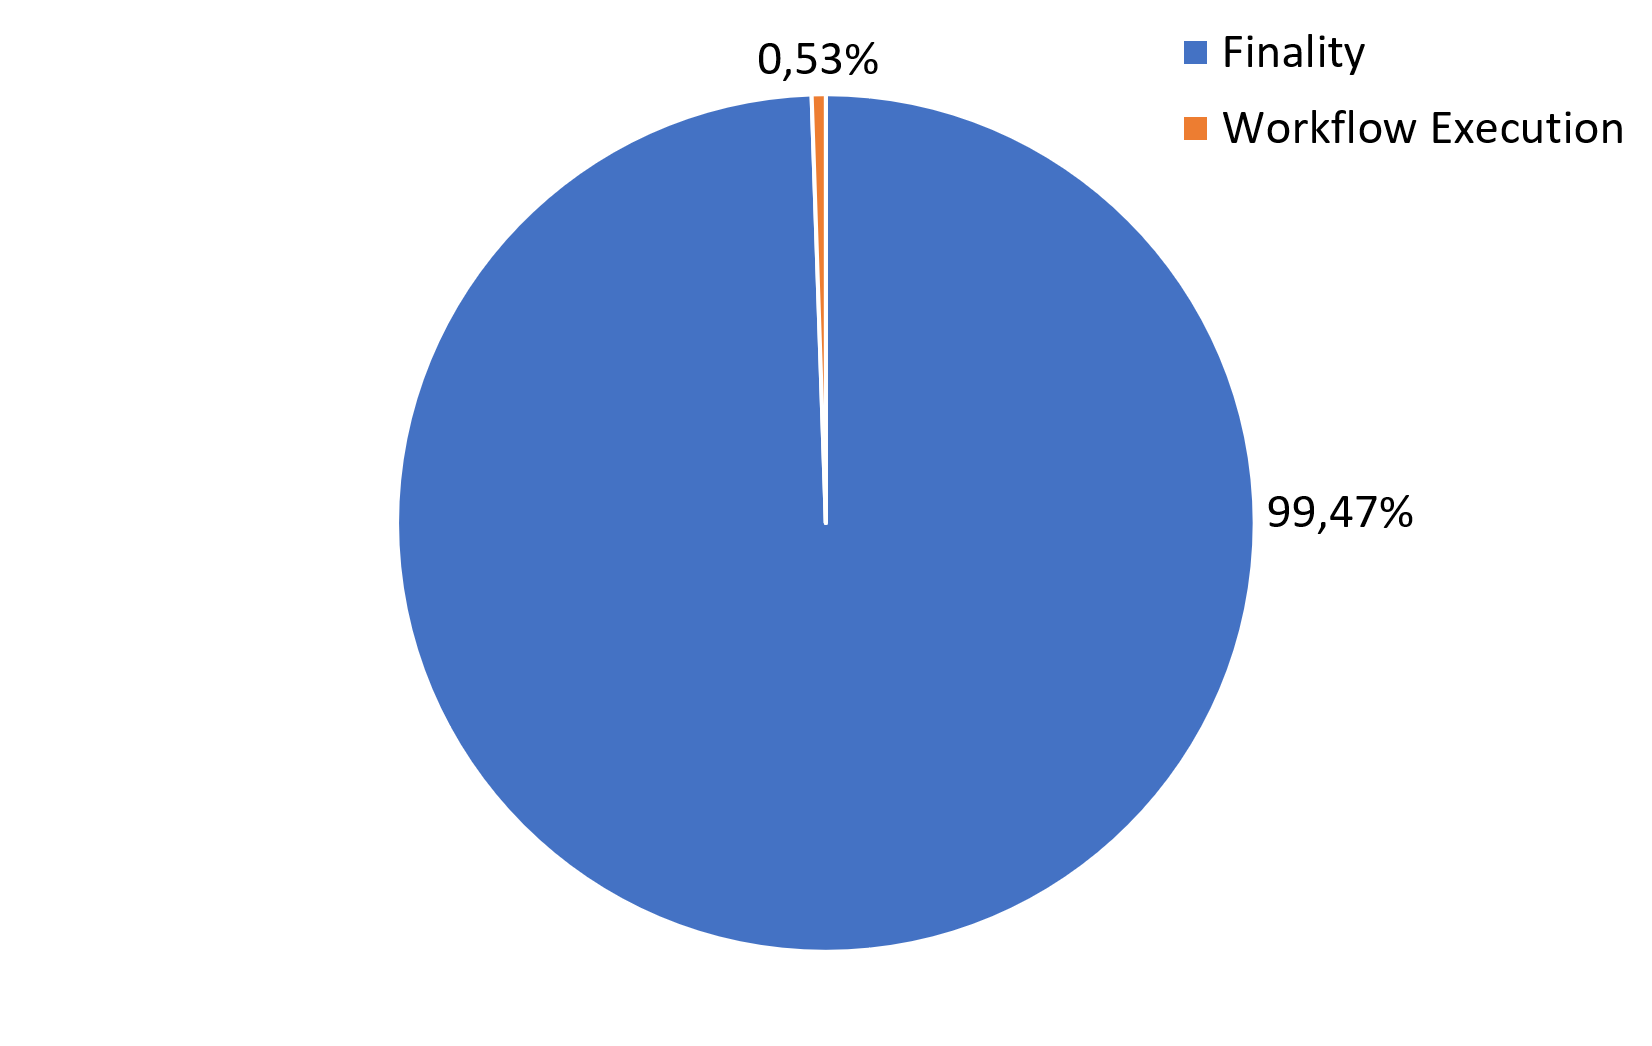
\includegraphics[width=.75\textwidth]{evaluation/graphics/experimental-analysis/finality-portion-pie-chart.png}}
    \caption{Pie chart illustrating a significant increase in workflow execution duration due to enforced transaction inclusion on the blockchain.}
    \label{fig:evaluation:simulations:pie_chart_transaction_inclusion_portion}
\end{figure}

Relying on enforced transaction inclusion has a significant impact on practical usability. Therefore, it should primarily be used for moderately to slow-paced workflows (requiring no more than 2 to 3 state transitions per minute). On the other hand, optimistic execution should only be used for very fast-paced workflows (more than four state transitions per minute), where little to no conflicts are expected. Fast-paced workflows that do produce conflicts between participants (due to conflicting rules being employed on each side, for example) must expect frequent rollbacks, which halts execution for a brief moment. Another scenario applicable for optimistic execution are tasks that only involve one participant because no two parties can disagree on a new workflow state\footnote{This also includes workflows only consisting of single party tasks (i.e.,\ entirely private workflows).}.

Nonetheless, it must be noted that these observations are only applicable when relying on an Ethereum-based consistency strategy. Optimistic execution might not even be considered viable when employing a strategy that, for example, leverages on a layer-2 rollup because the transaction inclusion duration is short enough to be neglected in the first place. Compared to existing approaches, a \gls{ttsm} with an \gls{evm}-based strategy typically performs between 20\%~\cite{untrusted_bp_execution_using_blockchain} and 25-times~\cite{runtime_verification_for_bp_utilizing_bitcoin} better regarding execution duration.

\subsubsection{Execution Cost}
\label{sec:evaluation:simulations:execution_cost}
Unlike execution duration, execution cost is tightly coupled with the number of participants involved in a certain operation, as discussed in the static analysis in section~\ref{sec:evaluation:static_analysis:blockchain_transactions}. Even though the cost of creating a workflow definition, an instantiation of such, and performing state transitions is linear in growth, deploying the required smart contract that stores the hashes of these operations remains constant. The evaluation for execution cost was conducted according to the methodologies used by Weber et al.~\cite{untrusted_bp_execution_using_blockchain,optimized_execution_of_bp_using_petri_nets_on_blockchain}, López-Pintado et al.~\cite{interpreted_bp_on_blockchain_weber}, Sturm et al.~\cite{lean_architecture_for_blockchain_based_process_execution}, Loukil et al.~\cite{interpreted_bp_on_blockchain_loukil}.

Table~\ref{tab:evaluation:simulations:gas_cost} shows the gas cost of each operation for each of the three scenarios. Given that the supply chain and incident management scenarios have the same number of participants but a different number of tasks (see table~\ref{tab:evaluation:simulations:structural_comparison}), one clearly identifies a strong correlation. The increasing costs come from the two-step process that each operation has to go through: (1) proposing a new definition, instantiation, or state transition, and (2) requiring all participants to send an accept or reject message.

\begin{table}[h]
\centering
\begin{tabular}{|l|c|}
    \hline
    & \multicolumn{1}{c|}{\bfseries Facility Management} \\ \cline{2-2}
    & Op.\ gas cost \\
    \hline
    Smart Contract         & 95,337 \\
    Workflow Definition    & 68,502 \\
    Workflow Instantiation & 68,502 \\
    State Transition       & 68,502 \\
    \hline
    & \multicolumn{1}{c|}{\bfseries Supply Chain} \\ \cline{2-2}
    & Op.\ gas cost \\
    \hline
    Smart Contract         & 95,337  \\
    Workflow Definition    & 137,004 \\
    Workflow Instantiation & 137,004 \\
    State Transition       & 137,004 \\
    \hline
    & \multicolumn{1}{c|}{\bfseries Incident Management} \\ \cline{2-2}
    & Op.\ gas cost \\
    \hline
    Smart Contract         & 95,337  \\
    Workflow Definition    & 137,004 \\
    Workflow Instantiation & 137,004 \\
    State Transition       & 137,004 \\
    \hline
\end{tabular}
\caption{Total gas cost of each operation type per scenario}
\label{tab:evaluation:simulations:gas_cost}
\end{table}

Even though the cost for a single blockchain transaction is rather small, with 22,834 gas, scenarios involving a lot of participants may be at a disadvantage. Nonetheless, the \gls{ttsm} prototype still performs better cost-wise than most other interpreted~\cite{interpreted_bp_on_blockchain_loukil,interpreted_bp_on_blockchain_weber}, and far better than most compiled approaches~\cite{untrusted_bp_execution_using_blockchain,optimized_execution_of_bp_using_petri_nets_on_blockchain} considering the three scenarios described above. Table~\ref{tab:evaluation:simulations:gas_cost_total} summarizes the total execution cost of each scenario, including smart contract deployment (even though only required once), workflow definition, instantiation, and all state transitions where each state transition is dispatched to every participant.

\begin{table}[h]
\centering
\begin{tabular}{|l|r|}
    \hline
    \textbf{Scenario} & \textbf{Total gas cost} \\
    \hline
    Facility Management & 574,851 \\
    Supply Chain        & 1,739,385 \\
    Incident Management & 1,602,381 \\
    \hline
\end{tabular}
\caption{Total gas cost of each scenario}
\label{tab:evaluation:simulations:gas_cost_total}
\end{table}

Notice that the total cost is still relatively high even though smart contract deployment is much more cost-efficient compared to existing approaches~\cite{interpreted_bp_on_blockchain_loukil,interpreted_bp_on_blockchain_weber}. This gives an opportunity for future work to improve the concept of a \gls{ttsm} by decoupling the execution cost from the number of involved participants. In particular, two areas for further research have been identified:

\begin{itemize}
    \item Investigation of applicable techniques to reduce the number of participants involved in an operation to a minimum\footnote{Only the middleman and the carrier have to accept or reject a state transition if supplier, manufacturer, and buyer are not involved in this process step, for example.}.
    \item Investigation of applicable blockchain-oriented software design patterns that allow decoupling of execution cost and the number of participants.
\end{itemize}

The first research challenge might require an in-depth analysis of statecharts and concepts such as the one proposed by Nakamura et al.~\cite{inter_organizational_bps_managed_by_blockchain}, where the interaction between participants is split into multiple statecharts. An interesting approach for the latter one, on the other hand, might be the off-chain signatures design pattern where all involved participants sign a proposed operation before writing the hash of the operation itself and the signatures to the blockchain~\cite{eberhardt17off_block,weber2019_architecture_for_dapps_blockchain_patterns}. Others, such as Carminati et al.~\cite{blockchain_for_secure_io_bp}, or Sun et al.~\cite{sun2021_survey_of_zkp_on_blockchain} motivate the usage of \glspl{zkp}, homomorphic encryption, or \glspl{tee} for concepts similar to a \gls{ttsm} in order to improve privacy and confidentiality and, regarding the challenges mentioned above, to reduce execution cost. Nonetheless, the proposed concept and the \gls{ttsm} prototype have shown their viability for use in real-world scenarios by demonstrating a rather low overall execution cost and exhibiting the potential for future improvements.

\subsubsection{Practical Conflict Resolution}
\label{sec:evaluation:simulations:conflict_resolution}
Scenarios such as the supply chain example described in section~\ref{sec:evaluation:simulations:descriptions:sc} are typically prone to create conflicts between participants. Resolving these, however, is rather trivial when properly employing a \gls{ttsm} due to its consistency, persistence, and verifiability properties. To demonstrate this, a conflict was simulated for the supply chain scenario, where a deadline was not met. It was successfully resolved by leveraging the time-travelling capabilities of the proposed concept and the prototype. By going back in time, the exact moment when delays were introduced was identified by the corresponding blockchain commitment reference. The hashes stored on-chain were then compared to the hashes of the operations stored off-chain. Therefore, the conflict was resolved by determining who introduced the delays by utilizing the auditability property of the blockchain.

\subsubsection{Privacy and Flexibility}
\label{sec:evaluation:simulations:privacy_flexbility}
Privacy was demonstrated thoroughly throughout the simulation of all three scenarios. All data is stored in hashed form on the blockchain when using the \gls{evm}-strategy. Therefore, even on public blockchains, only participants involved in the workflow can read and verify workflow-specific data. Leveraging on the concept's flexibility, future work may replace the \gls{evm}-strategy with a strategy based on \glspl{zkp}, layer-2 rollups, or homomorphic encryption, for example. Strategies like these hold potential regarding sharing and proving specific properties fulfilled by private workflow tasks without exposing confidential information~\cite{blockchain_for_secure_io_bp,sun2021_survey_of_zkp_on_blockchain}. Especially rollups, where many try to establish \gls{evm} compatibility, would enable the portability of the proposed approach and the smart contract presented in code listing~\ref{lst:evaluation:simulations:hash_storage}. Throughout the prototype implementation and evaluation, different strategies were employed to demonstrate the consistency module's flexibility. Nonetheless, metadata, such as hashes or \glspl{zkp}, still end up on the blockchain. Solving this issue is a topic for future research, especially regarding GDPR compliance.

% FOR REFERENCE
%\cite{untrusted_bp_execution_using_blockchain} & - & 334,646 & -\\
%\cite{optimized_execution_of_bp_using_petri_nets_on_blockchain} & - & 322,154 & -\\
%\cite{interpreted_bp_on_blockchain_weber} & 3,365,098 & 721,049 & \\
%\cite{lean_architecture_for_blockchain_based_process_execution} & - & 1,036,085\\
%\cite{interpreted_bp_on_blockchain_loukil} & 3,643,898 & 995,754\\


% \begin{itemize}
    % \item Use the facility maintenance use case to show that even a prototype of a \gls{ttsm} can handle real world business processes.
    % \item Experimental analysis using EVM because its portable
    % \item Solidity-ByteCode converter for layer-2 rollups
    % \item Is waiting for finality (i.e. latency) really practical? see \cite{untrusted_bp_execution_using_blockchain}
    % \item What about the cost? see \cite{untrusted_bp_execution_using_blockchain}
    % \item Only easy scenarios with prototype for evaluation. (Maybe use use cases from \cite{untrusted_bp_execution_using_blockchain})
    % \item Gas cost in paper \cite{interpreted_bp_on_blockchain_weber}
    % \item off-chain signature pattern might improve this even further!\cite{eberhardt17off_block,weber2019_architecture_for_dapps_blockchain_patterns}
    % \item Metrics might be: Execution cost, latency
    % \item SHOULD demonstrate real-world utility
% \end{itemize}



\section{Integration with Camunda's Zeebe}
\label{sec:evaluation:integration}
An aspect unneglectable in Design Science research is showing real-world utility of the produced artifacts~\cite{hevner2004_design_science}. One facet not discussed in this context until now is the integration of a \gls{ttsm} into an existing and well-established \gls{bpm} system to improve practical acceptance\footnote{Exchanging an existing solution with a new one is often times more complex and time consuming than integrating one into the other.}. Therefore, this section briefly introduces a possible adaptation of the existing \gls{ttsm} prototype in order to integrate it with Camunda's\footnote{\href{https://camunda.com/}{Camunda Website} (accessed on 2022-10-29)} workflow execution engine Zeebe\footnote{\href{https://docs.camunda.io/docs/components/zeebe/zeebe-overview/}{Camunda Docs: Zeebe} (accessed on 2022-10-29)}, to then discuss further opportunities. Camunda cloud\footnote{\href{https://console.cloud.camunda.io/}{Camunda Cloud Console} (accessed on 2022-10-29)} was used to provide access to instances of Camunda and Zeebe.


\subsection{Prototype Adaptations}
\label{sec:evaluation:integration:adaptations}
An integration requires some minor adaptations in the form of extensions to the prototype. The \textit{open-closed principle}, that the proposed concept for a \gls{ttsm} strictly follows, together with the modular design and the established event bus system, make it straightforward to create and attach new subsystems~\cite{meyer97_oo_software_construction,martin96_open_closed_principle,geirhos2015_design_patterns}. A new module called \textit{IntegrationsModule} has been added, to enable participants to dynamically integrate workflows and workflow instances into existing \gls{bpm} systems. It determines during runtime and, based on a given configuration which integrations to use. Furthermore, it also exposes the new \textit{ZeebeModule}. The \textit{ZeebeModule} is solely commissioned with the interaction between the \gls{ttsm} prototype and Camunda's Zeebe workflow execution engine. It stores its local data in the form of event logs as part of the global event bus and accesses it by aggregation by using projections\footnote{This is similar to the behavior of the rules module, for example.}. For the interaction between the prototype and Zeebe, the \textit{ZeebeModule} relies on the \textbf{zeebe-node 8.1.2}\footnote{\url{https://npmjs.com/package/zeebe-node} (accessed on 2022-11-29)} NodeJS library which allows the implementation of hooks that are triggered by Zeebe using gRPC\@. The code that links a \gls{ttsm} workflow instance with a Zeebe process instance is shown in listing~\ref{lst:evaluation:integration:zeebe_job_worker}.\\

\begin{lstlisting}[language=JavaScript,caption=Implementation of dynamic Zeebe job worker registration,captionpos=b,label=lst:evaluation:integration:zeebe_job_worker]
async linkProcessInstance(instance: WorkflowInstanceProposal) {

  // Job worker function to advance TTSM workflows.
  const handler: ZBWorkerTaskHandler = (job: ZeebeJob) => {
    try {
      this.workflowService.advanceWorkflowInstance(
        instance.id,
        {
          event: job.type,
          payload: job.variables
        }
      );
    } catch (error) {
      return job.fail(error.message);
    }
    return job.complete();
  };

  // Each workflow has a list of state names (strings).
  for (const nextStateName of instance.workflow.states) {

    // Register a job worker for each consistency task.
    this.zeebeClient.createWorker({
      taskType: nextStateName,
      taskHandler: handler
    });
  }
}
\end{lstlisting}

The \textit{ZeebeModule} creates a new worker for each state in the given workflow. Whenever a participant advances the state inside Camunda, the corresponding worker is triggered and either returns a \textit{fail} or \textit{complete} response to Zeebe. Note that this is only a basic prototypical implementation of such an integration that should serve as proof of concept. It is not part of the actual \gls{ttsm} concept itself. In a full-fledged implementation, the \textit{ZeebeModule} should await inclusion of the transaction into a block on the blockchain before returning a response and notify all participants to keep the workflow state synchronized. The adaptations described above are also available on GitHub\footnote{\url{https://github.com/danielkleebinder/ttsm-prototype} (accessed on 2022-11-29)}.

% \begin{itemize}
    % \item New module ``ZeebeModule'' that stores its local data in the event store and projection aggregates data.
    % \item Workflow definitions are deployed on Zeebe every time a \textbf{\textit{Consistency.Workflow.Received}} internal persistence event is detected.
    % \item Workflow instances are deployed on Zeebe every time a \textbf{\textit{Consistency.Instance.Received}} internal persistence event is detected.
    % \item Zeebe client for NodeJS has been used.
    % \item Zeebe connection might be integrated into workflow instantiation
    % \item Very basic prototypical implementation. The ``ZeebeModule'' should probably only complete a job if it has a commitment reference on the blockchain and all participants are aware of the state transition.
    % \item This implementation is only a proof of concept!!! And not part of the actual \gls{ttsm} concept.
% \end{itemize}

\subsection{Workflow Execution}
\label{sec:evaluation:integration:execution}
In order to leverage on the properties of a \gls{ttsm}, the \gls{bpmn} diagrams used in Camunda must follow a certain format. Each task in Camunda that wants to interact with the \gls{ttsm} must be defined as a ``service task'' to trigger a job worker. These are tasks dedicated to ensure consistency and traceability using a \gls{ttsm} and mark the interfaces between participants. An example of such a \gls{bpmn} diagram is given in figure~\ref{fig:evaluation:integration:service_tasks}.

\begin{figure}[h]
    \makebox[\textwidth][c]{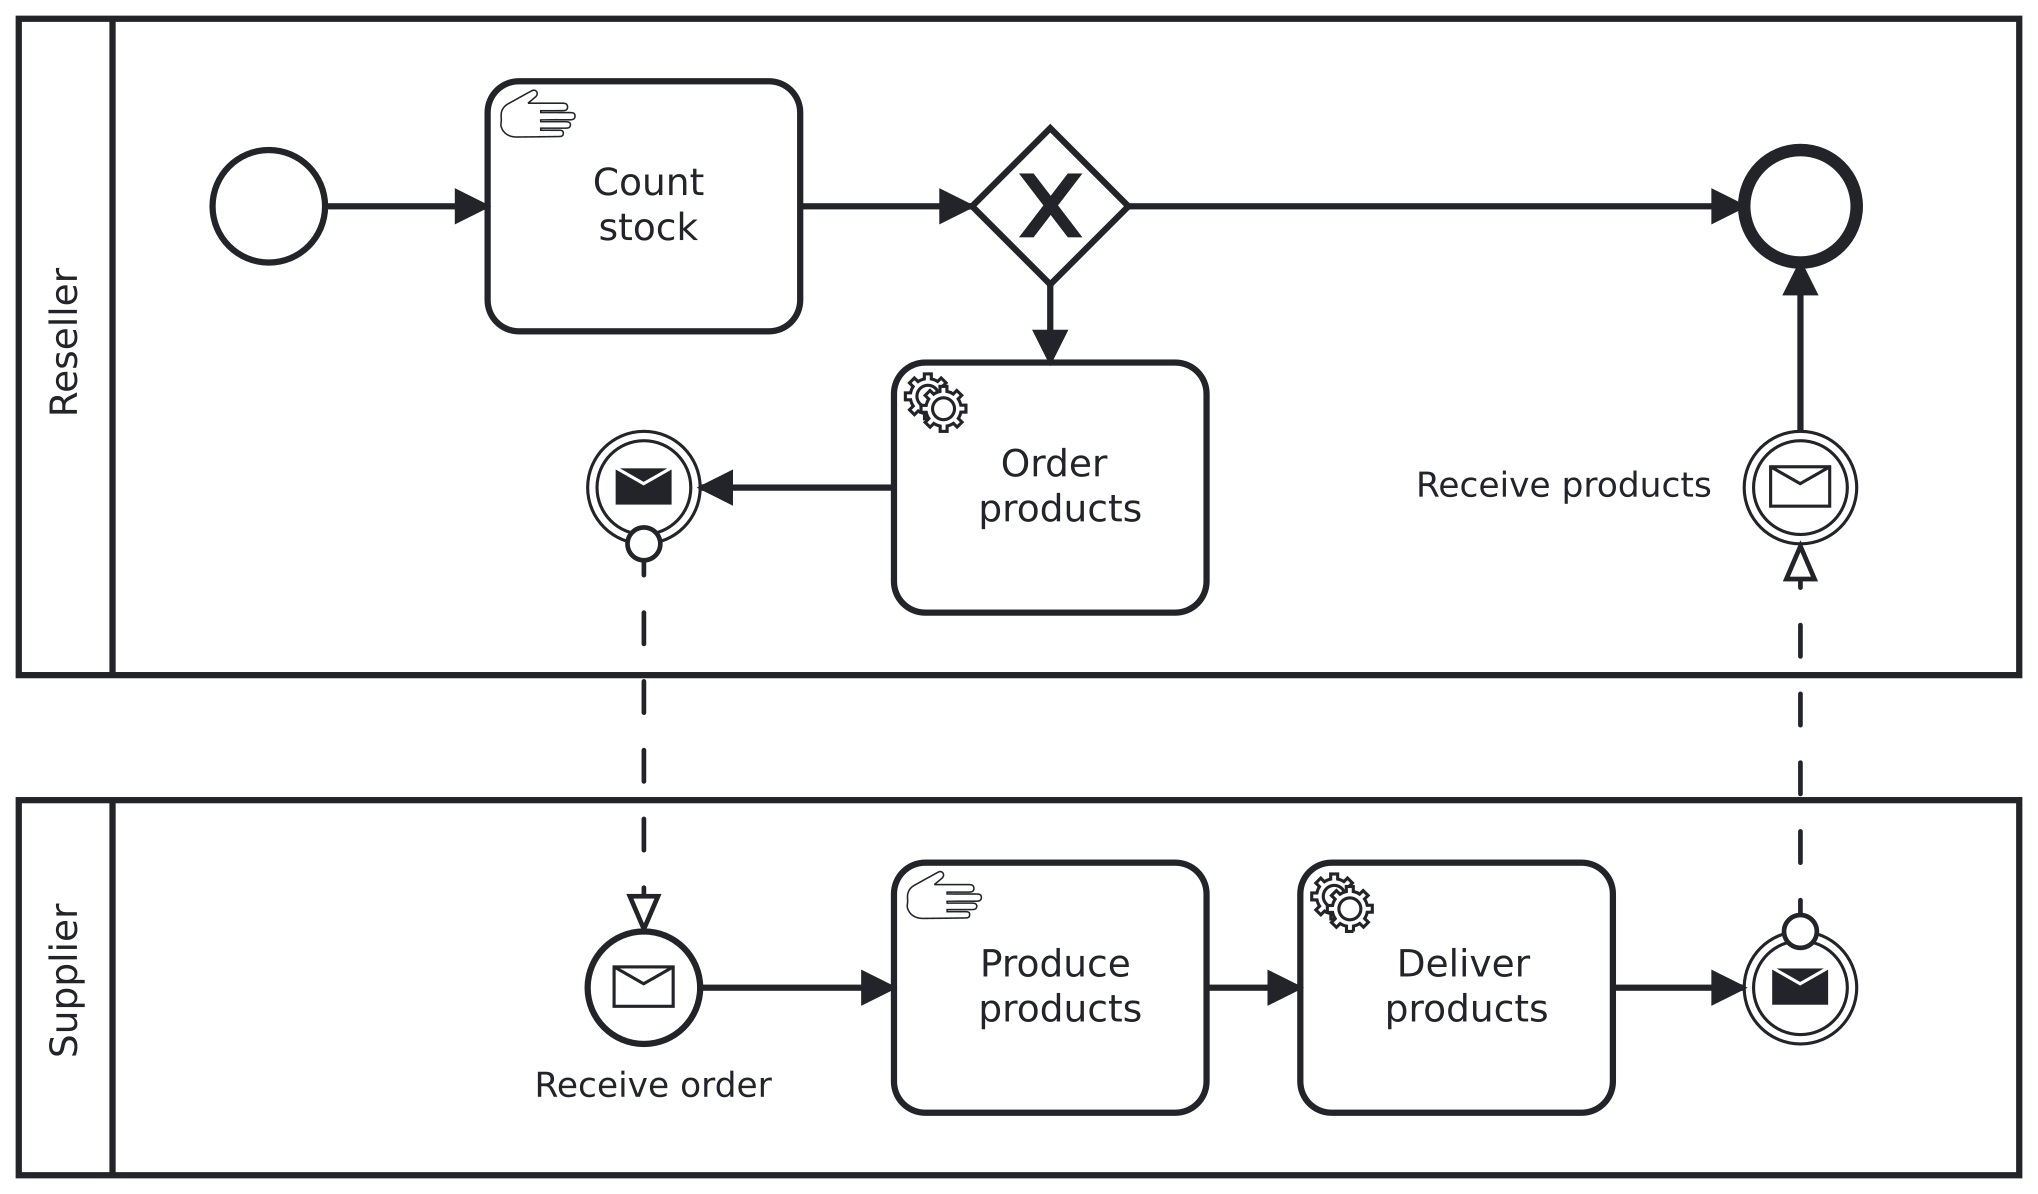
\includegraphics[width=.7\textwidth]{evaluation/graphics/integration/camunda-supplier-reseller.png}}
    \caption{Exemplary reseller-supplier scenario with service tasks before each interaction.}
    \label{fig:evaluation:integration:service_tasks}
\end{figure}

A reseller counts her stock and, depending on the result, orders products from the supplier. The ``Order products'' activity is a service task that triggers a \gls{ttsm} job worker, which handles the consistency concerns and the interaction between participants. After the supplier received the order and produced all required products, the deliver products service task is invoked, eventually leading to product delivery and completing the workflow. For the \gls{ttsm} to properly interact with Camunda and Zeebe, a choreography diagram solely concerned with the interactions between participants must be derived. Such an integration-compliant diagram only contains the service tasks and the names of the participants. Other activities are treated as private. A dedicated consistency service task must be specified if private activities require consistency. This means that service tasks that trigger a job worker in a \gls{ttsm} are not limited to interactions between two or more participants; however, they are predestined for it. Private service tasks require choreography activities to specify the same party as initiator and receiver. Figure~\ref{fig:evaluation:integration:service_tasks_choreography} shows the choreography diagram of the reseller-supplier scenario from figure~\ref{fig:evaluation:integration:service_tasks} above.

\begin{figure}[h]
    \makebox[\textwidth][c]{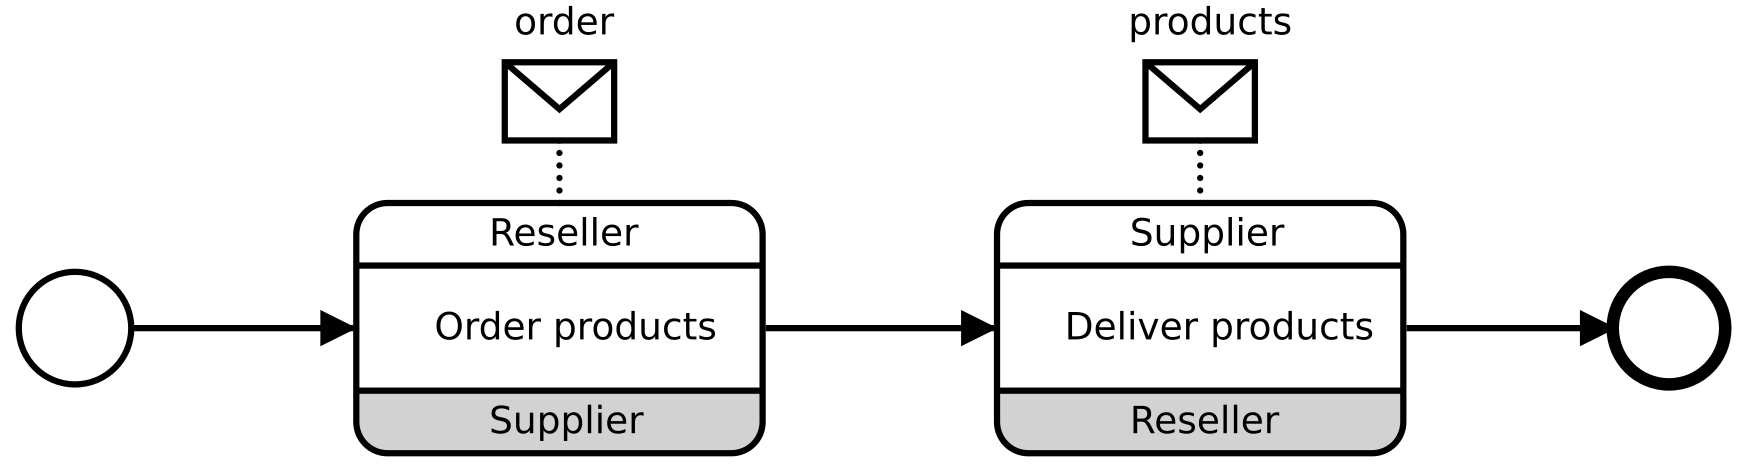
\includegraphics[width=.7\textwidth]{evaluation/graphics/integration/camunda-supplier-reseller-choreography.png}}
    \caption{Choreography of the reseller-supplier scenario.}
    \label{fig:evaluation:integration:service_tasks_choreography}
\end{figure}

This choreography diagram is then converted to statecharts and deployed by the \gls{ttsm}. Even though the deployment and instantiation are directly executed on the \gls{ttsm}, the workflow instance execution is performed using the graphical UI of Camunda. All necessary configuration of the Zeebe-integration is part of the deployment and the instantiation of the workflow.

% \begin{itemize}
    % \item Each task in Camunda that wants to interact with the \gls{ttsm} must be defined as ``service task'' to allow a job worker to be triggered. Dedicated tasks for consistency so to say.
    % \item Deployment and instantiation of a workflow must be executed by the \gls{ttsm}, state transitions are then performed by Zeebe inside Camunda.
    % \item Requires converter from statecharts to Zeebe-compliant \gls{bpmn} diagrams (hard-coded at the moment).
    % \item State transitions must be defined as Zeebe task definitions as an extension to standard \gls{bpmn}.
% \end{itemize}

\subsection{Summary and Discussion}
\label{sec:evaluation:integration:summary}
The evaluation performed in this section has introduced some minor extensions to the \gls{ttsm} prototype by adding a \textit{ZeebeModule} for integration into Camunda's Zeebe workflow execution engine. It allows participants to execute workflow instances using the graphical UI of Camunda while keeping auditability, traceability, and consistency properties of a \gls{ttsm}. However, the integration of workflow deployment was not possible. The evaluation of Camunda connectors\footnote{\href{https://docs.camunda.io/docs/components/integration-framework/connectors/use-connectors/}{Camunda Docs: Connectors} (accessed on 2022-10-29)} and Zeebe job workers\footnote{\href{https://docs.camunda.io/docs/components/concepts/job-workers/}{Camunda Docs: Job Workers} (accessed on 2022-10-29)} shows that they are no suitable solutions, because they are not concerned with the entirety of the workflow, but only with single tasks. This yields the following research challenge for future work:

\begin{itemize}
    \item Investigation of integration strategies that allow participants to deploy and instantiate new workflows using Camunda and its underlying workflow execution engine Zeebe instead of relying on the \gls{ttsm}.
\end{itemize}

Answering this research challenge might include writing a custom Camunda plugin\footnote{\href{https://docs.camunda.org/how-tos/cockpit/develop-a-plugin/}{Camunda Docs: Custom Plugins} (accessed on 2022-10-29)}. Nonetheless, the integration seems to hold great potential. Therefore, a more in-depth investigation considering the integration of a \gls{ttsm} into Camunda and Zeebe is advised as part of future work. This might include replacing parts of the Zeebe or Camunda architectures with concepts proposed in this work or vice versa by replacing the workflow module with Zeebe, for example. Even though the integration evaluation in this work has only been a proof of concept with very little functionality, it demonstrated interesting prospects that future work could leverage on.

% \begin{itemize}
    % \item A more in-depth investigation is advised considering \gls{ttsm}-integration into Camunda and Zeebe.
    % \item Integration seems to hold great potential
    % \item Workflow module can be replaced with Zeebe, for example
% \end{itemize}

\subsection{Research Question 3}
\label{sec:evaluation:integration:rq3}
To answer the third research question:

\begin{quote}
    \emph{Which aspects must be adapted to close the gap between the state of the art and a privacy-preserving \gls{bct}-based state machine that allows time-travel verification?}
\end{quote}

Existing workflow execution systems already hold great potential when it comes to the integration of the concept for a \gls{ttsm}. Not only is this a viable option when auditability or traceability are required, but the expenditure for such a venture also seems to be relatively low. Concepts proposed in related work that leverage on blockchains, however, have shown a formidable lack of flexibility and privacy. This can be traced back to the fact that almost all concepts rely on running code directly on layer-1 blockchains. Even though some concepts aim to circumnavigate or even solve the shortcomings imposed by layer-1 blockchains, neither can mitigate the majority of them. To close the gap between the state of the art and a privacy-preserving \gls{bct}–based state machine that allows time-travel verification, future concepts might want to start building on layer-2 or even start targeting layer-2 rollups and build on layer-3 instead of directly leveraging on blockchains. Using the blockchain as a supportive third-party system that provides certain properties increases the flexibility of the system built on top of it and reduces its cost. Nonetheless, the potential imposed by a \gls{bct}–based state machine that only takes advantage of blockchain properties without directly building, and thus constraining itself by it, is not to be neglected.

% This, however, might require future work to identify desirable layer-1 properties, which properties layer-2 or layer-3 applications must fulfill, and which layer-1 properties can be transferred to layer-2 or layer-3 without canceling out desirable properties from underlying layers.


% \begin{itemize}
    % \item Do not use layer-1 blockchains, build on layer-2 or even better on layer 3.
% \end{itemize}


\chapter{Conclusion}
\label{sec:conclusion}

Computer-aided \gls{bpm} is a hot topic for both industrial and research communities. With the uprise of blockchains in recent years, the latter started an endeavor towards blockchain-based \gls{bpm} to leverage on one of its unique properties of \glspl{bct} --- trust. Organizations and companies can now cooperate with each other without the need for a centralized, trusted third party. Nonetheless, research has been following a strict trend where software has been tightly coupled to the underlying blockchain resulting in a lack of flexibility and privacy. By performing a narrative literature review and applying design science, this work created a novel concept for building \gls{bpm} systems that take advantage of the properties blockchains provide without restricting themselves by their shortcomings.

The concept proposes a four-module architecture where each module ensures specific properties. The \textit{workflow module} is solely responsible for the creation and execution of workflows. By extending its interface, it can support a vast range of different \gls{bp} modeling languages and is, therefore, very much declarative; a desirable property regarding the practical value of such systems. As the second one, the \textit{rules module} allows participants to verify if rules beyond simple workflow semantics are fulfilled. The third module, the \textit{consistency module}, provides an abstract interface to the underlying \gls{bct}. There are no strict requirements for this module. Usage of the Bitcoin network is as viable as the usage of layer-2 rollups, for example. The last module provides persistent storage and a convenient interface that allows participants to time travel between different workflow states. During the course of this work, the concept was continuously evaluated against qualitative metrics and predefined \glspl{bp} to constantly improve its practicality.

The evaluation has shown significant traits regarding flexibility without forfeiting trust, traceability, or auditability provided by the underlying \gls{bct}. This was traced back to the \gls{ttsm} operating one layer above the \gls{bct} without requiring tight coupling; a characteristic that has not yet been investigated in much detail in related literature. This allows for a highly modular architecture where components are only loosely coupled, interchangeable and extensible, resulting in a list of advantages, including the option to switch between blockchains if needed, dynamic participant selection, or adjusting the workflow structure while being executed. Furthermore, during the execution of exemplary scenarios, it has been shown that, depending on the requirements of the participants, privacy can be fully preserved or only in parts if needed. In what detail conflicts between participants can be resolved then weakly correlates with the level of privacy.

Additionally, the proposed concept also reduces the overall execution cost of workflows. For the scenarios simulated in the evaluation, the \gls{ttsm} prototype performed better than most existing solutions. However, the cost correlates linearly with the number of participants involved and will break even if this number exceeds a certain threshold. Nonetheless, there are promising \gls{bose} software design patterns that can solve this issue. Further investigation in future work is advised.

Even though introducing an architecture that separates the blockchain and the workflow execution engine increases the system's complexity to some extent, it brings forth desirable properties, as mentioned above. Related literature and existing solutions, however, broadly introduce a tight coupling between both. Therefore, future work might want to investigate further into building blockchain-based \gls{bpm} systems as layer-2 or layer-3 applications instead of directly leveraging on the blockchain and running code on layer-1. However, this requires preliminary work identifying desirable layer-1 properties and how they can be transferred and used on layer-2 or layer-3. In this context, one might extend and leverage upon the \textit{consistency module} as proposed in this work.

Another topic future work should extend upon is the investigation of compensation mechanisms for lost peer-to-peer or even peer-to-blockchain connections. Solving this problem from the distributed systems domain further improves resiliency of the choreography but requires preliminary research of algorithms with small on-chain footprint that enables participants to verify the integrity of messages exchanged between participants.

% The proposed concept internally operates upon statecharts to execute workflow logic. This requires conversion is required to support diagrams created with different modeling languages. Even though ground laying work already exists that describes reduction algorithms from UML sequence diagrams or process models to statecharts, algorithms for \gls{bpmn} are still missing. Resolving this open problem will further increase practical acceptance of the proposed approach because participants no longer have to manually convert diagrams to statecharts which is potentially error-prone.

Regarding the integration into other systems, a couple of open problems are still to answer. One is the handling of large or exotically structured payloads in state transitions. They cannot be part of the \textit{persistence module} itself because it would clutter storage and transfer potentially unnecessary information between participants. A solution one might investigate is \textit{content-addressable storage} where only the reference to the data is exchanged and stored on-chain. Another aspect to consider is the integration into existing \gls{bpm} systems. Even though the integration into Camunda's Zeebe workflow execution engine has been shown to be viable during the evaluation, a thorough investigation is still outstanding.

Nonetheless, the idea of a \gls{ttsm} that operates off-chain, but leverages upon the unique properties of \glspl{bct}, has been demonstrated. Especially improved flexibility is a trait future systems might build upon. This work should be considered as a starting point for \gls{bpm} systems that take advantage of the blockchain as a source of trust, traceability, and auditability while treating it as a loosely coupled sub-system of supportive nature.


% \subsubsection{Improvements}
% \label{sec:conclusion:future_work:improvements}

% \begin{itemize}
    % \item Open problem: Investigation of applicable techniques to reduce the number of participants involved in an operation to a minimum\footnote{Only the middleman and the carrier have to accept or reject a state transition if supplier, manufacturer and buyer are not involved in this process step, for example.}.
    % \item Open problem: Investigation of applicable blockchain-oriented software design patterns that allow decoupling of execution cost and the number of participants.
    % \item Open problem: The investigation of algorithms with a small on-chain footprint that enables participants the verify message integrity (see \ref{sec:evaluation:static_analysis:summary}).
    % \item Open problem: the investigation of compensation mechanisms for lost peer-to-peer or even peer-to-blockchain connections to further increase resiliency (see \ref{sec:evaluation:static_analysis:summary}).
    % \item Open problem: Figuring out the details of optimistic execution is up to future work (see \ref{sec:evaluation:simulations:execution_duration}).
    % \item Translators: How to convert choreography and BPMN diagrams to state charts?
    % \item Workflow instances cannot be modified during execution.
    % \item On-demand workflow instance participant selection (technically possible as an extension).
    % \item Authentication issue of participants could be solved by signing contracts that someone truly is being a certain wallet for example.
    % \item Multi-chain support to make discussion chapter more interesting (already described in section \ref{sec:ttsm:proposal:entering_blockchain_and_distributing_commands} to some extent as well)?
% \end{itemize}


% \subsubsection{Integrations}
% \label{sec:conclusion:future_work:integrations}

% \begin{itemize}
    % \item Handling of large payloads: Possible solution is to  only transmit references to Speckle\footnote{\url{https://speckle.systems/}} or content-addressable storage\footnote{\url{https://en.wikipedia.org/wiki/Content-addressable_storage}} commits?
    % \item Availability and resiliency of the sub-systems: The consistency module and all sub-systems including the event store and the blockchain need some level of availability because dropped messages and error cases are still not answered.
    % \item Rules Module: The details of the rules module, how it time travels, how and what it verifies and how users specify rules is still open.
    % \item Internal-activities are handled by local systems (participant specifying entire workflow, does not know of internal-activities of all other participants) in discussion.
% \end{itemize}


% \chapter{Cool Stuff}
% \section{How to write a thesis}
This section is just a collection of links, tips and tricks on how to write a thesis and how to stay motivated.

\subsection{Stupid Question: Why is Writing a Thesis So Hard?}
\begin{quote}
    ``For me, the hardest thing was getting the structure and story right. Second hardest was staying motivated and concentrating. For the structure, the best thing I found when I was struggling (and tbh, even when I wasn't) was to break it down into headings, subheadings, subsubheadings, etc. Work out roughly what you want the point of a paragraph to be. Jot down sentences as bullet points of keywords if you need to. Don't just sit down to write and expect it to flow. Sometimes you'll write things and need to move them around, but it's much easier to try and work out the flow of the story in advance. This also helps with motivation, because it's naturally broken down into small manageable chunks so it's much easier to progress.''
\end{quote}

\begin{itemize}
    \item Stick to your proposal, it's a major milestone and answers a lot of questions.
\end{itemize}

\url{https://www.reddit.com/r/GradSchool/comments/f4p41p/stupid_question_why_is_writing_a_thesis_so_hard/}

\subsection{Submission}
Some links regarding master thesis submission at the TU Vienna:

\begin{itemize}
    \item \url{https://informatics.tuwien.ac.at/study-services/dates/#master-diplomprüfung}
    \item \url{https://informatics.tuwien.ac.at/study-services/master-graduation/}
\end{itemize}

\section{Interesting Papers}
The following list of papers and references was used to introduce the author to the topics of consensus, offchain vs onchain and the baseline protocol. It is ordered going from broad references that introduce one to a topic to very specific topics that require some knowledge from previous references.

\subsection{Designing Data-Intensive Applications}
The author gives a sophisticated introduction to consensus mechanisms and why they are important for distributed systems based on a lot of references and research papers.

\textbf{Martin Kleppmann}~\cite{kleppmann17desig} (p.364--375)

\subsection{The Byzantine Generals Problem}
This paper introduces the reader to the Byzantine Generals Problem and proves in a quite understandable fashion that a computer system with $n \leq 3f$ nodes cannot be trusted if $f$ nodes are faulty.

\textbf{Leslie Lamport, Robert Shostak, Marshall Pease}~\cite{lamport2002}

\subsection{Impossibility of distributed consensus with one faulty process}
The famous paper from Fischer et al.\ that won the Dijkstra price for being one of the most influential papers in distributed systems in the recent years. The authors impressively show that, in a purely asynchronous (deterministic) system, you cannot have safety, liveliness and fault-tolerance properties of a consensus protocol all at once.

\textbf{Michael J. Fischer, Nancy A. Lynch, Michael S. Paterson}~\cite{impossibility_result_1985}

\subsection{Practical Byzantine Fault Tolerance}
Barbara Liskov and Miguel Castro show the first practical implementation of an asynchronous Byzantine fault tolerant algorithm using NFS and introduce the reader to concepts like liveliness and safety properties.

\textbf{Barbara Liskov, Miguel Castro}~\cite{liskov1999}

\subsection{The latest gossip on BFT consensus}
Tendermint is a BFT consensus algorithm that uses the foundation and concepts built by PBFT and applies them to the blockchain by changing the way proposers (i.e.\ ``leaders'') are elected and views are changed.

\textbf{Ethan Buchman, Jae Kwon, Zarko Milosevic}~\cite{tendermint2018}

\subsection{State Machine Replication for the Masses with BFT-SMART}
This paper shows how the BFT-SMART framework was implemented, which difficulties the authors had to face and how they guarantee improved reliability with modularity and crash tolerance besides the built in Byzantine fault tolerance.

\textbf{Alysson Bessani, Joao Sousa, Eduardo E. P. Alchieri}~\cite{bessani14state_machin_replic_masses_bft_smart}

\subsection{From Byzantine Consensus to BFT State Machine Replication: A Lateny-Optimal Transformation}
The authors show in detail how the MOD-SMART module of the BFT-SMART framework was implemented and how they achieved latency and resiliency optimization in their algorithm.

\textbf{Alysson Bessani, Joao Sousa}~\cite{sousa12from_byzan_consen_bft_state_machin_replic}

\subsection{Stumbling over Consensus Research: Misunderstandings and Issues}
The author of this paper tries to close the gap between theoretical consensus research and practical use. He states, that practitioners often misunderstand some of the theoretical concepts in consensus and thus frequently miss some opportunities.

\textbf{Marcos K. Aguilera}~\cite{aguilera2010}

\subsection{Bitcoin: A Peer-to-Peer Electronic Cash System}
The original whitepaper of Bitcoin by Satoshi Nakamoto written in quite easily understandable fashion that outlines the core principles of Bitcoin very well.

\textbf{Satoshi Nakamoto}~\cite{nakamoto2009}

\subsection{Majority is not enough: Bitcoin mining is vulnerable}
This paper introduces the reader to the concept of ``Selfish Mining'' which can be used on proof-of-work based blockchains to increase the revenue from mining by a degree that is usually not intended.

\textbf{Ittay Eyal, Emin Gün Sirer}~\cite{eyal2013}

\subsection{A Next-Generation Smart Contract and Decentralized Application Platform}
The original whitepaper of Ethereum by Vitalik Buterin. It contains the concepts on which Ethereum relys on and explains them quite understandably.

\textbf{Vitalik Buterin}~\cite{buterin2020}

\subsection{Blockchain without Waste: Proof-of-Stake}
One of the original scientific papers about proof of stake that shows disadvantages of proof of work blockchains and how proof of stake could improve upon this.

\textbf{Fahad Saleh}~\cite{proof_of_stake}

\subsection{Applicability and Appropriateness of Distributed Ledgers Consensus Protocols in Public and Private Sectors: A Systematic Review}
A profound review and comparison of all consensus protocols available at the time the paper was written. It ranges from proof of work to PBFT and Tendermint even considering rather exotic variations like Magi's proof of stake or proof of spacetime.

\textbf{A. Shahaab, B. Lidgey, C. Hewage, I. Khan}~\cite{consensus_comparison_2019}

\subsection{Cambridge Bitcoin Electricity Consumption Index}
A web-platform that shows the total amount of energy consumed by Bitcoin and includes some interesting comparisons with countries and others.

\textbf{Cambridge University}~\cite{cbeci}

\subsection{On or Off the Blockchain? Insights on Off-Chaining Computation and Data}
A great paper outlining the advantages and disadvantages of off-chaining in the context of Ethereum. The authors introduce 5 new interesting patterns on off-chaining computation and storage.

\textbf{Jacob Eberhardt, Stefan Tai}~\cite{eberhardt17off_block}

\subsection{Off-chaining Models and Approaches to Off-chain Computations}
The authors give motivation to off-chaining storage and computation and introduce some off-chain computation approaches that allow users to keep certain data private but still be able to interact with blockchains (be it in the form of zero-knowledge proofs or TEEs).

\textbf{Jacob Eberhardt, Jonathan Heiss}~\cite{eberhardt18off_model_approac_off_comput}

\subsection{Towards Blockchain Tactics: Building Hybrid Decentralized Software Architectures}
A systematic method for designing Blockchain applications is required. The authors showcase this circumstance using a simple example where gas cost of an Ethereum smart contract diverges dramatically depending on the use case.

\textbf{Florian Wessling, Christopher Ehmke, Ole MEyer, Volker Gruhn}~\cite{towards_blockchain_tactics}

\subsection{Building Hybrid DApps using Blockchain Tactics: The Meta-Transaction Example}
Meta-transactions are transactions towards EDCC that are signed by the creator of the transaction but sent to the blockchain by some other third party. This paper shows different approaches to meta-transactions and what the differences between strategies, tactics and design patterns are.

\textbf{Florian Blum, Benedikt Severin, Michael Hettmer, Philipp Hückinghaus, Volker Gruhn}~\cite{building_hybrid_dapps_using_blockchain_tactics}

\subsection{How much Blockchain do you need? Towards a Concept for building hybrid DApp Architectures}
Deciding upon the macro-architecture of a software application is no trivial task. Especially, because most blockchain applications are so complex, that not all parts require direct blockchain interaction. This paper shows a systematic method on how to determine which parts of an architecture require blockchain technology and which do not.

\textbf{Florian Wessling, Christopher Ehmke, Marc Hesenius, Volker Gruhn}~\cite{how_much_blockchain_do_you_need}

\subsection{Engineering Software Architectures of Blockchain-Oriented Applications}
Which options do users have when interacting with the blockchain? This paper answers this question and compares the three options by security, trust and convenience aspects.

\textbf{Florian Wessling, Volker Gruhn}~\cite{engineering_software_architectures_of_BO_Apps}

\subsection{Blockchain-oriented Software Engineering: Challenges and new Directions}
The authors motivate the reader by listing some million dollar mistakes made from incorrect software engineering on blockchain applications, that a systematic approach is needed and show some challenges based on blockchain technology.

\textbf{Andrea Pinna, Michele Marchesi, Roberto Tonelli}~\cite{blockchain_oriented_software_engineering}

\subsection{Making Smart Contracts Smarter}
The authors give a basic introduction to consensus and smart contracts in Ethereum and continue with common vulnerabilities and attack vectors and show how one might circumvent them.

\textbf{Loi Luu, Duc-Hiep Chu, Hrishi Olickel, Prateek Saxena, Aquinas Hobor}~\cite{making_smart_contracts_smarter}

\subsection{A Survey of Tools for Analyzing Ehtereum Smart Contracts}
Very interesting paper about the available tooling for analyzing Ethereum smart contracts from Monika di Angelo and Gernot Salzer from TU Wien with insight on what is currently possible, what not and what developers of such tool should consider.

\textbf{Monika di Angelo, Gernot Salzer}~\cite{tools_for_analyzing_smart_contracts}


% \chapter{Meetings}
% \section{2021.07.30}

Read and research on:
\begin{itemize}
\item Consensus
  \begin{itemize}
  \item From Byzantine Consensus to BFT State Machine Replication~\cite{sousa12from_byzan_consen_bft_state_machin_replic}
  \item State Machine Replication for the Masses with BFT-SMART~\cite{bessani14state_machin_replic_masses_bft_smart}
  \item Designing Data intensive applications~\cite{kleppmann17desig} (p. 364 to p. 375)
\end{itemize}
\item On-Off chain
  \begin{itemize}
  \item Off-Chain Models~\cite{eberhardt18off_model_approac_off_comput}
  \item On- or Off-chain~\cite{eberhardt17off_block}
  \end{itemize}
\item baseline
  \begin{itemize}
  \item \url{https://docs.baseline-protocol.org/}
  \item \url{https://github.com/eea-oasis/baseline/tree/master/core}
\end{itemize}
\end{itemize}
Practical:
\begin{itemize}
\item test baseline reference implementation
  \begin{itemize}
  \item \url{https://docs.baseline-protocol.org/bri/bri-1}
  \item \url{https://docs.baseline-protocol.org/bri/bri-2}
  \end{itemize}
\end{itemize}

\section{2021.08.06}
Short update, same to-does as last week.
These additional consensus paper could be relevant or interesting:
\begin{itemize}
\item Hotstuff (libra consenus bft) \url{https://arxiv.org/abs/1803.05069}
\item Bitcoin selfish mining paper \url{https://dl.acm.org/doi/pdf/10.1145/3212998}
\item Avalanche consensus \url{https://arxiv.org/abs/1906.08936}
\item Tendermint consensus \url{https://arxiv.org/abs/1807.04938}
\item Algorand consensus \url{https://www.sciencedirect.com/science/article/pii/S030439751930091X}
\end{itemize}

\section{2021.08.13}
Paper consensus algorithms comparison: \url{https://ieeexplore.ieee.org/abstract/document/8672572}

\begin{itemize}
\item Consensus properties (wikipedia/kleppman/\ldots)
\item State machine replication
\item Finality
\item Blockchain specifics
  \begin{itemize}
  \item Public /private
  \item permissioned / permissionless
  \end{itemize}
\end{itemize}

\section{2021.08.20}
To-Does from last week.

\section{2021.08.27}
Most things from the last few meetings are done. Open To-Does:
\begin{itemize}
\item Rework text as we talked (references, paragraphs, etc.)
\item Extend Onchain and offchain section by methods
\item Look at papers on Blockchain application development by Florian
  Blum. \url{https://florianblum.com/research} Write about your
  findings.
\item Look into Baseline and try out the reference implementations.
\end{itemize}

\section{2021.09.10}
Open To-Does and references:
\begin{itemize}
\item Write section based on papers from Florian Blüm.
\item minted package for code highlighting (\url{https://ctan.org/pkg/minted?lang=de})
\item Kleppman talk on Kafka/DBs (\url{https://www.youtube.com/watch?v=fU9hR3kiOK0})
\item Baseline conference EthAtlanta (\url{https://ethatl.com/})
\item Provide (\url{https://provide.services/}) and stack docs (\url{https://docs.provide.services/api/})
\end{itemize}

\section{2021.09.17}
Transactional Patterns und Hybrid Apps fertig schreiben

Baseline und Provide Stack:
\begin{itemize}
\item In Baseline und Provide einlesen und einarbeiten
\item Baseline-Protokoll Slack-Channel beitreten
\item (Später eventuell auch 2 oder 3 Seiten zum Baseline Protokoll schreiben)
\end{itemize}

Referenzen nochmal durchschauen:
\begin{itemize}
\item Die Einträge von BibTex nochmal ansehen. Nicht alle Einträge (z.B. ``journal'' bei ``@misc'') werden gerendert.
\item Bei Links und Online-Resourcen (wie ``@misc'') wie Ethereum Whitepaper ``publisher'' statt ``journal'' verwenden
\item Bei ``@inproceedings'' sind ``pages'' und ``publisher'' wichtig
\item ``journal'' oder ``booktitle'' hinzufügen
\item Bei ``@inbook'' werden Kapitel von Büchern referenziert
\end{itemize}

Expose bzw. Proposal vorbereiten und Gedanken zum konkreten Thema der Arbeit machen:
\begin{itemize}
\item Wie bringt man die Blockchain zum User ohne Blockchain?
\item Blockchain-oriented Processmanagement (UI zum Benutzer hin)
\item Mitte Oktober mit etwas Projekterfahrung weiter besprechen
\end{itemize}


Überlegen ob mit VM, Laptop oder lokalem PC und remote arbeiten
Erster Arbeitstag am 04.10.

(Apache Kafka und Samza eventuell Stichwort-mäßig ein bisschen beschreiben)

\section{2021.12.13}
\label{sec:2021.12.13}

Topics:
\begin{itemize}
\item Systematic literature review on BPMN and Blockchain (send paper)
\item Caterpillar (send paper!)

\end{itemize}

Research Questions (draft):
\begin{itemize}
\item Entwurf eines Konzepts wie eine Historical State Machine als Businessprozess konfiguriert werden kann.
\item Entwurf eines Konzepts zur historischen Datenspeicherung von großen Datensets.
\item Entwurf eines Konzepts wie große Datensets vor Veränderung (Tamperproofness) geschützt werden können.
\end{itemize}

topic brainstorming:
\begin{itemize}
\item (general vs. in baseline context)?
\item cross-organisational bpm
\item workflow engine
\item historical; logs; transcripts
\item blockchain/smart contract/distributed ledger technologies/web3
\item baseline
\item associated data
\end{itemize}

\emph{Translation:}
How can a concept for a historical state machine for distributed business process management be implemented.

Possible questions for the concept/approach/method:
\begin{itemize}
\item What are the requirements?
\item What data has to be saved/changed?
\item How can changes be logged?
\item What data has to be linked?
\item What about event sourcing?
\end{itemize}

Method/approach for a efficient baseline compliant state machine that
fulfills the requirements and constraints.

\emph{Evaluation:} Prototype implementation for elevator use case

\textbf{Draft research questions:}
\begin{enumerate}
\item What is the state of the art in distributed state machines for business process management workflow engines?
\item Which approach or aspects are the most suitable/are required for baseline and what is missing?
  \begin{enumerate}
  \item How can the approaches/aspects be adapted to close the gap?
  \end{enumerate}
\end{enumerate}


To-Does:
\begin{itemize}
\item Search methodology for literature review
\item Search methodology for design science part (Hevner)
\item Outline for proposal
\end{itemize}

%%% Local Variables:
%%% mode: latex
%%% TeX-master: "thesis"
%%% End:

\section{2022.05.16}
What happened since the last meeting?
\begin{itemize}
    \item Worked myself through A LOT of literature
    \item Defined literature review methodology
    \item Defined basic outline for time-travelling state machines
\end{itemize}

Questions:
\begin{itemize}
    \item Should I put my methodology into its own chapter or should I move it to the chapter where it was used?
    \begin{itemize}
        \item Either own chapter or as subsection in chapter.
    \end{itemize}
    \item \textit{Same question as above for the research questions.}
    \item Number of references per number of words (like 8 to 12 for 1000 words?!?!)
    \begin{itemize}
        \item Should be somewhere between 50 and 100 references
    \end{itemize}
    \item How do I justify that I "chose the papers that I think are applicable for my thesis"?
    \begin{itemize}
        \item Do not necessarily describe this. Take too much time and already goes into the field of SLR. Maybe keep a list of literature with reasons why I didnt choose a certain paper just in case someone criticizes the work later one.
    \end{itemize}
    \item More ideas for concept comparison?
    \begin{itemize}
        \item On- vs. off-chain. What data is on- and what is off-chain?
        \item Describe fields of concept comparison.
    \end{itemize}
    \item What time should I use?
    \begin{itemize}
        \item No future!
        \item Related work mainly with past and present tense, rest with present tense.
    \end{itemize}
    \item Where to put source code and listings? Maybe into the evaluation?
    \begin{itemize}
        \item Longer source codes in Appendix, else try to shorten code and put it where it fits best.
    \end{itemize}
\end{itemize}

To-Does:
\begin{itemize}
    \item Further describe methodology, how many search results, filtered by headlines and abstract.
    \item More keywords:
    \begin{itemize}
        \item CAP-Theorem for consistency (e.g. \url{https://jepsen.io/consistency})
        \item Consistency as open (distributed systems) question
        \item Design science in approach
        \item BP book from Mathias Weske \url{https://link.springer.com/book/10.1007/978-3-642-28616-2} for BP background section
    \end{itemize}
    \item Describe the scope of the work and where the cuts are.
    \item Think about concept for rule engine integration
    \item Add pro and cons for artifact- vs. BP-centric approach
    \item Script tasks in \url{https://link.springer.com/chapter/10.1007/978-3-030-26619-6_7}. Also extends choreography diagrams with very interesting examples on GitHub
    \item Take a look at ZK-Circuits in Baseline Protocol standard and check how they store state
    \item Architecture and sequence diagram of state machine with modules
    \item \textbf{Does BPMN 2.0 and \url{https://link.springer.com/chapter/10.1007/978-3-030-26619-6_7} comply with Baseline Protocol and what aspects do we need to adept}
\end{itemize}


\section{2022.05.30}
What happened since the last meeting?
\begin{itemize}
    \item
\end{itemize}

Questions:
\begin{itemize}
    \item
\end{itemize}

To-Does:
\begin{itemize}
    \item Feel \url{https://camunda.github.io/feel-scala/docs/reference/}
    \item TrustMesh \url{https://docs.baseledger.net/baseledger-concepts/trustmesh}
\end{itemize}


\section{2022.07.25}
What happened since the last meeting?
\begin{itemize}
    \item Written introduction to ``Business Process Managament''
    \item Defined facility management use case in more detail
    \item Written ``Business Process Model and Notation'' subsection
    \item Written ``Orchestration and Choreography'' subsection
    \item Written ``Baseline Protocol'' section
    \item Added journals to related work methodology description
    \item Written ``Modeling and Enforcing Blockchain-Based Choreographies'' subsection in related work chapter
    \item Written ``Concept Comparison'' section
    \item Answered RQ1
\end{itemize}

Questions:
\begin{itemize}
    \item Do the \gls{bpmn} diagrams make sense in subsection ``Business Process Model and Notation''?
    \item Is the choreography diagram in subsection ``Orchestration and Choreography'' syntactically correct?
    \item Best approach to design science?
    \item Noticed any spelling or grammatical mistakes?
    \item What do you think of the Baseline Protocol section \ref{sec:background:baseline_protocol}? Is it sufficient? Should I go into more detail?
    \item How do I ignore Latex warnings only in certain occasions? (for citations for example)
\end{itemize}

To-Does:
\begin{itemize}
    \item[\checkmark] Loop in figure \ref{fig:background:maintenance_full} between report further defects and inspect maintenance
    \item[\checkmark] Check if letter symbol is required in BPMN
    \item[\checkmark] Simplify BPI in figure \ref{fig:background:maintenance_report_baseline} even more.
    \item[\checkmark] Baseline Protocol is still in heavy development and work in progress
    \item[\checkmark] ZKP are out of scope, make part of background of Baseline Protocol
    \item[\checkmark] On page 20, choreography tasks interact with two \textbf{or more} parties
    \item[\checkmark] ''The box itself contains the message exchanged`` should be replaced with ``the inside of the box describes...'' (Martin takes a closer look at this)
    \item[\checkmark] Look at proposal for introduction of Baseline Protocol (page 21).
    \item[\checkmark] Rethink introduction to Baseline Protocol using docs and FAQ. Baseline Protocol reduces flexibility but increases synchronization resiliency with blockchain (maybe use quotes).
    \item[\checkmark] Add architecture diagram (system of record communicates with BPI and nats and nats and BPI to system of record)
    \item[\checkmark] Remove ``Baseline Protocol'' from RQs
    \item[\checkmark] Use grammarly (see meeting on 2022.09.02)
    \item[\checkmark] Argument logically why some design decision was applied
    \item[\checkmark] Read Hevner and watch video from Martin
    \item[\checkmark] Why did I use Design Science?
\end{itemize}


\section{2022.09.02}
What happened since the last meeting?
\begin{itemize}
    \item Overhauled baseline protocol background section \ref{sec:background:baseline_protocol}
    \item Written about design science methodology and tailoring in section \ref{sec:ttsm:methodology}
    \item Written about the proposal in section \ref{sec:ttsm:proposal}
    \item Written introduction to prototype design section \ref{sec:ttsm:prototype}
    \item Defined outline of workflow layer subsection \ref{sec:ttsm:prototype:workflow_layer}
\end{itemize}

Questions:
\begin{itemize}
    \item Is it clear from the design science methodology section why I used design science in the first place?
    \item Can I use literature written in german language (Entwurfsmuster by Matthias Geirhos)?
    \item Is the proposal written precise enough?
    \item I did not describe each layer separately in section \ref{sec:ttsm:proposal}, but tried to tell the story of a single state transitions from being dispatched by one participant until it reaches consensus. Is this the best approach (Stichwort ``roter Faden'')?
    \item Grammarly can only analyse PDFs in paid version. Does TU Wien have any free premium licenses for students or just for such occasions?
    \item Is it okay, if my actual prototype implementation diverges a little bit from what I describe in my masters thesis in section \ref{sec:ttsm:prototype}?
\end{itemize}

To-Does:
\begin{itemize}
    \item[\checkmark] Send FMChain postman collections to Thomas
    \item[\checkmark] Read over background chapter and correct it
    \item Read over related work chapter and correct it
    \item[\checkmark] Rename ``Proposal'' to ``Concept'', ``Proposed Concept'' or something similar
    \item[\checkmark] Subsection in one line (maybe)
    \item[\checkmark] Invite Thomas to prototype GitHub
    \item[\checkmark] Design Science -- Guideline 7: Work is communication of research (look-up Hevner)
    \item Move CQRS from proposed concept to background section
    \item Grieving problem as part in discussion or evaluation from section \ref{sec:ttsm:proposal:reaching_consensus} open problem - needs workarounds
    \item Workflow should be designed that each participant should have incentive to accept state transition
    \item[\checkmark] Internal-activities are handled by local systems (participant specifying entire workflow, does not know of internal-activities of all other participants) in discussion
    \item[\checkmark] In discussion showing, that mathematical properties could be improved
    \item[\checkmark] Background chapter in Grammarly (can interpret LaTeX for free)
\end{itemize}


\section{2022.09.16}
What happened since the last meeting?
\begin{itemize}
    \item Written about prototype design.
    \item Written about qualitative evaluation.
    \item Written about network topology in static analysis.
\end{itemize}

Questions:
\begin{itemize}
    \item 
\end{itemize}

To-Does:
\begin{itemize}
    \item Experimental analysis is more of simulative nature
    \item Sentences are a bit long
    \item Tables and graphics are too wide
    \item Should the word ``taxonomy'' really be used? Martin will discuss this with Thomas. Maybe use ``classification'' instead.
    \item Maybe cite from where criteria come from.
    \item[\checkmark] Open question 2 in qualitative analysis is decentralized identity (did) problem (\url{https://www.w3.org/TR/did-core/}).
    \item[\checkmark] ``Future work has to solve'' to ``an open issue is...''
    \item[\checkmark] Rewrite banks example in section \ref{sec:evaluation:qualitative_analysis:privacy_criteria}
    \item The concept is very modular, may require architectural analysis
    \item[\checkmark] In section \ref{sec:evaluation:qualitative_analysis:summary} use ``transaction cost'' instead of ``the cost that blockchains produce''
    \item In section \ref{sec:evaluation:qualitative_analysis:summary}: the sentence ``For the most part, this can be traced back to the role of the blockchain that is only of supportive nature.'' is THE USP of my work!!!! Reference literature (none available that only uses the blockchain as support) review and cite on- and off-chain paper.
    \item Its modular!!
    \item The sentence ``For the most part, this can be traced back to the role of the blockchain that is only of supportive nature.'' also in conclusion
    \item[\checkmark] In section \ref{sec:evaluation:static_analysis}, $n$ is the number of participants involved in an activity.
    \item[\checkmark] Not all participants must sign a state transition!!! Important point!
\end{itemize}


\section{2022.10.06}
What happened since the last meeting?
\begin{itemize}
    \item Written introduction chapter.
    \item Completed static analysis (see section \ref{sec:evaluation:static_analysis})
    \item Really highlight the flexibility of the proposed approach (see section \ref{sec:evaluation:qualitative_analysis:summary})
    \item Thoughts about experimental evaluation: Module for third-party software just listens to EventStore events and adds new events
    \item Thoughts about experimental evaluation: Adapter for databases using a trigger that dispatches actions if certain fields change
    \item Described prototype adaptations for scenario simulations in section \ref{sec:evaluation:simulations:adaptations}
    \item Described three scenarios used for evaluation in section \ref{sec:evaluation:simulations:descriptions}.
    \item Checked related work chapter \ref{sec:related-work} with Grammarly.
\end{itemize}

Questions:
\begin{itemize}
    \item Thesis probably needs a math check, especially regarding the static analysis in section \ref{sec:evaluation:static_analysis} in the evaluation.
\end{itemize}

To-Does:
\begin{itemize}
    \item[\checkmark] Experimental analysis using EVM because its portable
    \item[\checkmark] Solidity-ByteCode converter for layer-2 rollups
    \item Use case on zkSync / starknet
    \item Camunda for existing solutions
    \item[\checkmark] Book: Architecture for Blockchain Applications
\end{itemize}


\section{2022.11.11}
What happened since the last meeting?
\begin{itemize}
    \item Finalized introduction (\ref{sec:introduction}).
    \item Finalized background chapter incoporated feedback from Thomas (\ref{sec:background}).
    \item Finalized related work chapter (\ref{sec:related-work}).
    \item Finalized theoretical section of the \gls{ttsm} chapter (\ref{sec:ttsm}).
    \item Completed the scenario simulations evaluation (\ref{sec:evaluation:simulations}).
    \item Completed the integration with Camundas' Zeebe evaluation (\ref{sec:evaluation:integration}).
    \item Answered RQ3 (\ref{sec:evaluation:integration:rq3}).
    \item Completed the conclusion (\ref{sec:conclusion}).
\end{itemize}

Questions:
\begin{itemize}
    \item What do you think of my closing words?
    \item Does the integration into Camundas' Zeebe make sense in this form?
    \item Are the code listing properly chosen and applicable? I didn't put them into the prototype design section \ref{sec:ttsm:prototype} because they are extensions that are not directly part of the concept but a small example of ``how easy'' it is to extend the \gls{ttsm}.
    \item Does my conclusion sound too modest or too ``haughty''? I feel like its almost a little bit too ``Einstein can keep his theory of relativity, look what I have accomplished!!''.
    \item Replaced almost all ``like'' in background section with ``such as'', ``similar'' or ``as''. Are these terms more formal?
\end{itemize}

To-Does:
\begin{itemize}
    \item Incorporate feedback from Thomas.
    \item Read \gls{ttsm} and evaluation chapter once again.
    \item Prepare all required documents.
    \item Create poster.
\end{itemize}


\section{2022.11.18}
What happened since the last meeting?
\begin{itemize}
    \item Fixed all chktex-errors.
    \item Written and finalized abstract in english and german.
\end{itemize}

Questions:
\begin{itemize}
    \item I don't want to fix the remaining issues, because I think they make things worse or are ``wrong'' errors. What to do?
\end{itemize}

To-Does:
\begin{itemize}
    \item Enable more chktex errors and check if I can fix them.
    \item Persistence module requires a certain "Abfolge" of events
    \item TTSM rolls back all inconsistent or invalid transaction (ruhig zu intrinsic properties)
    \item Fußnote, dass TTSM und BCT-based TTSM äquivalent sind
    \item "finality" ersetzen mit "transaction inclusion"
    \item Mit Evaluation anfangen und Variablennamen anpassen
    \item Füllwörter löschen
    \item Zeitform ins Präsens bringen
    \item Seite 114: Warum manche Samples 50 und manche 80 mal
\end{itemize}


\section{2022.11.24}
\begin{itemize}
    \item https://informatics.tuwien.ac.at/epilog/best-poster-award/ In-Design Testphase
\end{itemize}


\backmatter

% Use an optional list of figures.
\listoffigures % Starred version, i.e., \listoffigures*, removes the toc entry.

% Use an optional list of tables.
\cleardoublepage % Start list of tables on the next empty right hand page.
\listoftables % Starred version, i.e., \listoftables*, removes the toc entry.

% Use an optional list of alogrithms.
\listofalgorithms
\addcontentsline{toc}{chapter}{List of Algorithms}

% Use an optional list of code listings
\cleardoublepage % Start list of tables on the next empty right hand page.
\lstlistoflistings

% Add an index.
\printindex

% Add a glossary.
\printglossaries

% Add a bibliography.
\bibliographystyle{alpha}
\bibliography{thesis, introduction/introduction, background/background, related-work/related-work, proposed-concept/proposed-concept, evaluation/evaluation, conclusion/conclusion}

\end{document}
%%% Local Variables:
%%% mode: latex
%%% TeX-master: t
%%% End:
